%------------------------------%
%% ✎ Dylan (V1) %%%%%%%%% ✅ %%
%% ✎ Alain (V2) %%%%%%%%% ✅ %%
%% ✎ Dylan (V3) %%%%%%%%% ✅ %%
%------------------------------%

%%%%%%%%%%%%%%%%%%%%%%%%%%%%%%%%
% Chapter~6
\chapterheader{Application of the \Commas{Node-Place Model} in the Hauts-de-France Region}
\chapter
{Regional Modeling of the Degrees of Development and Integration between Nodes and the Planning of Expanded Station Areas
    \label{chap6:titre}
    }
    \begin{refsegment}

% Background Chapter~6
\AddToShipoutPictureBG*{%
  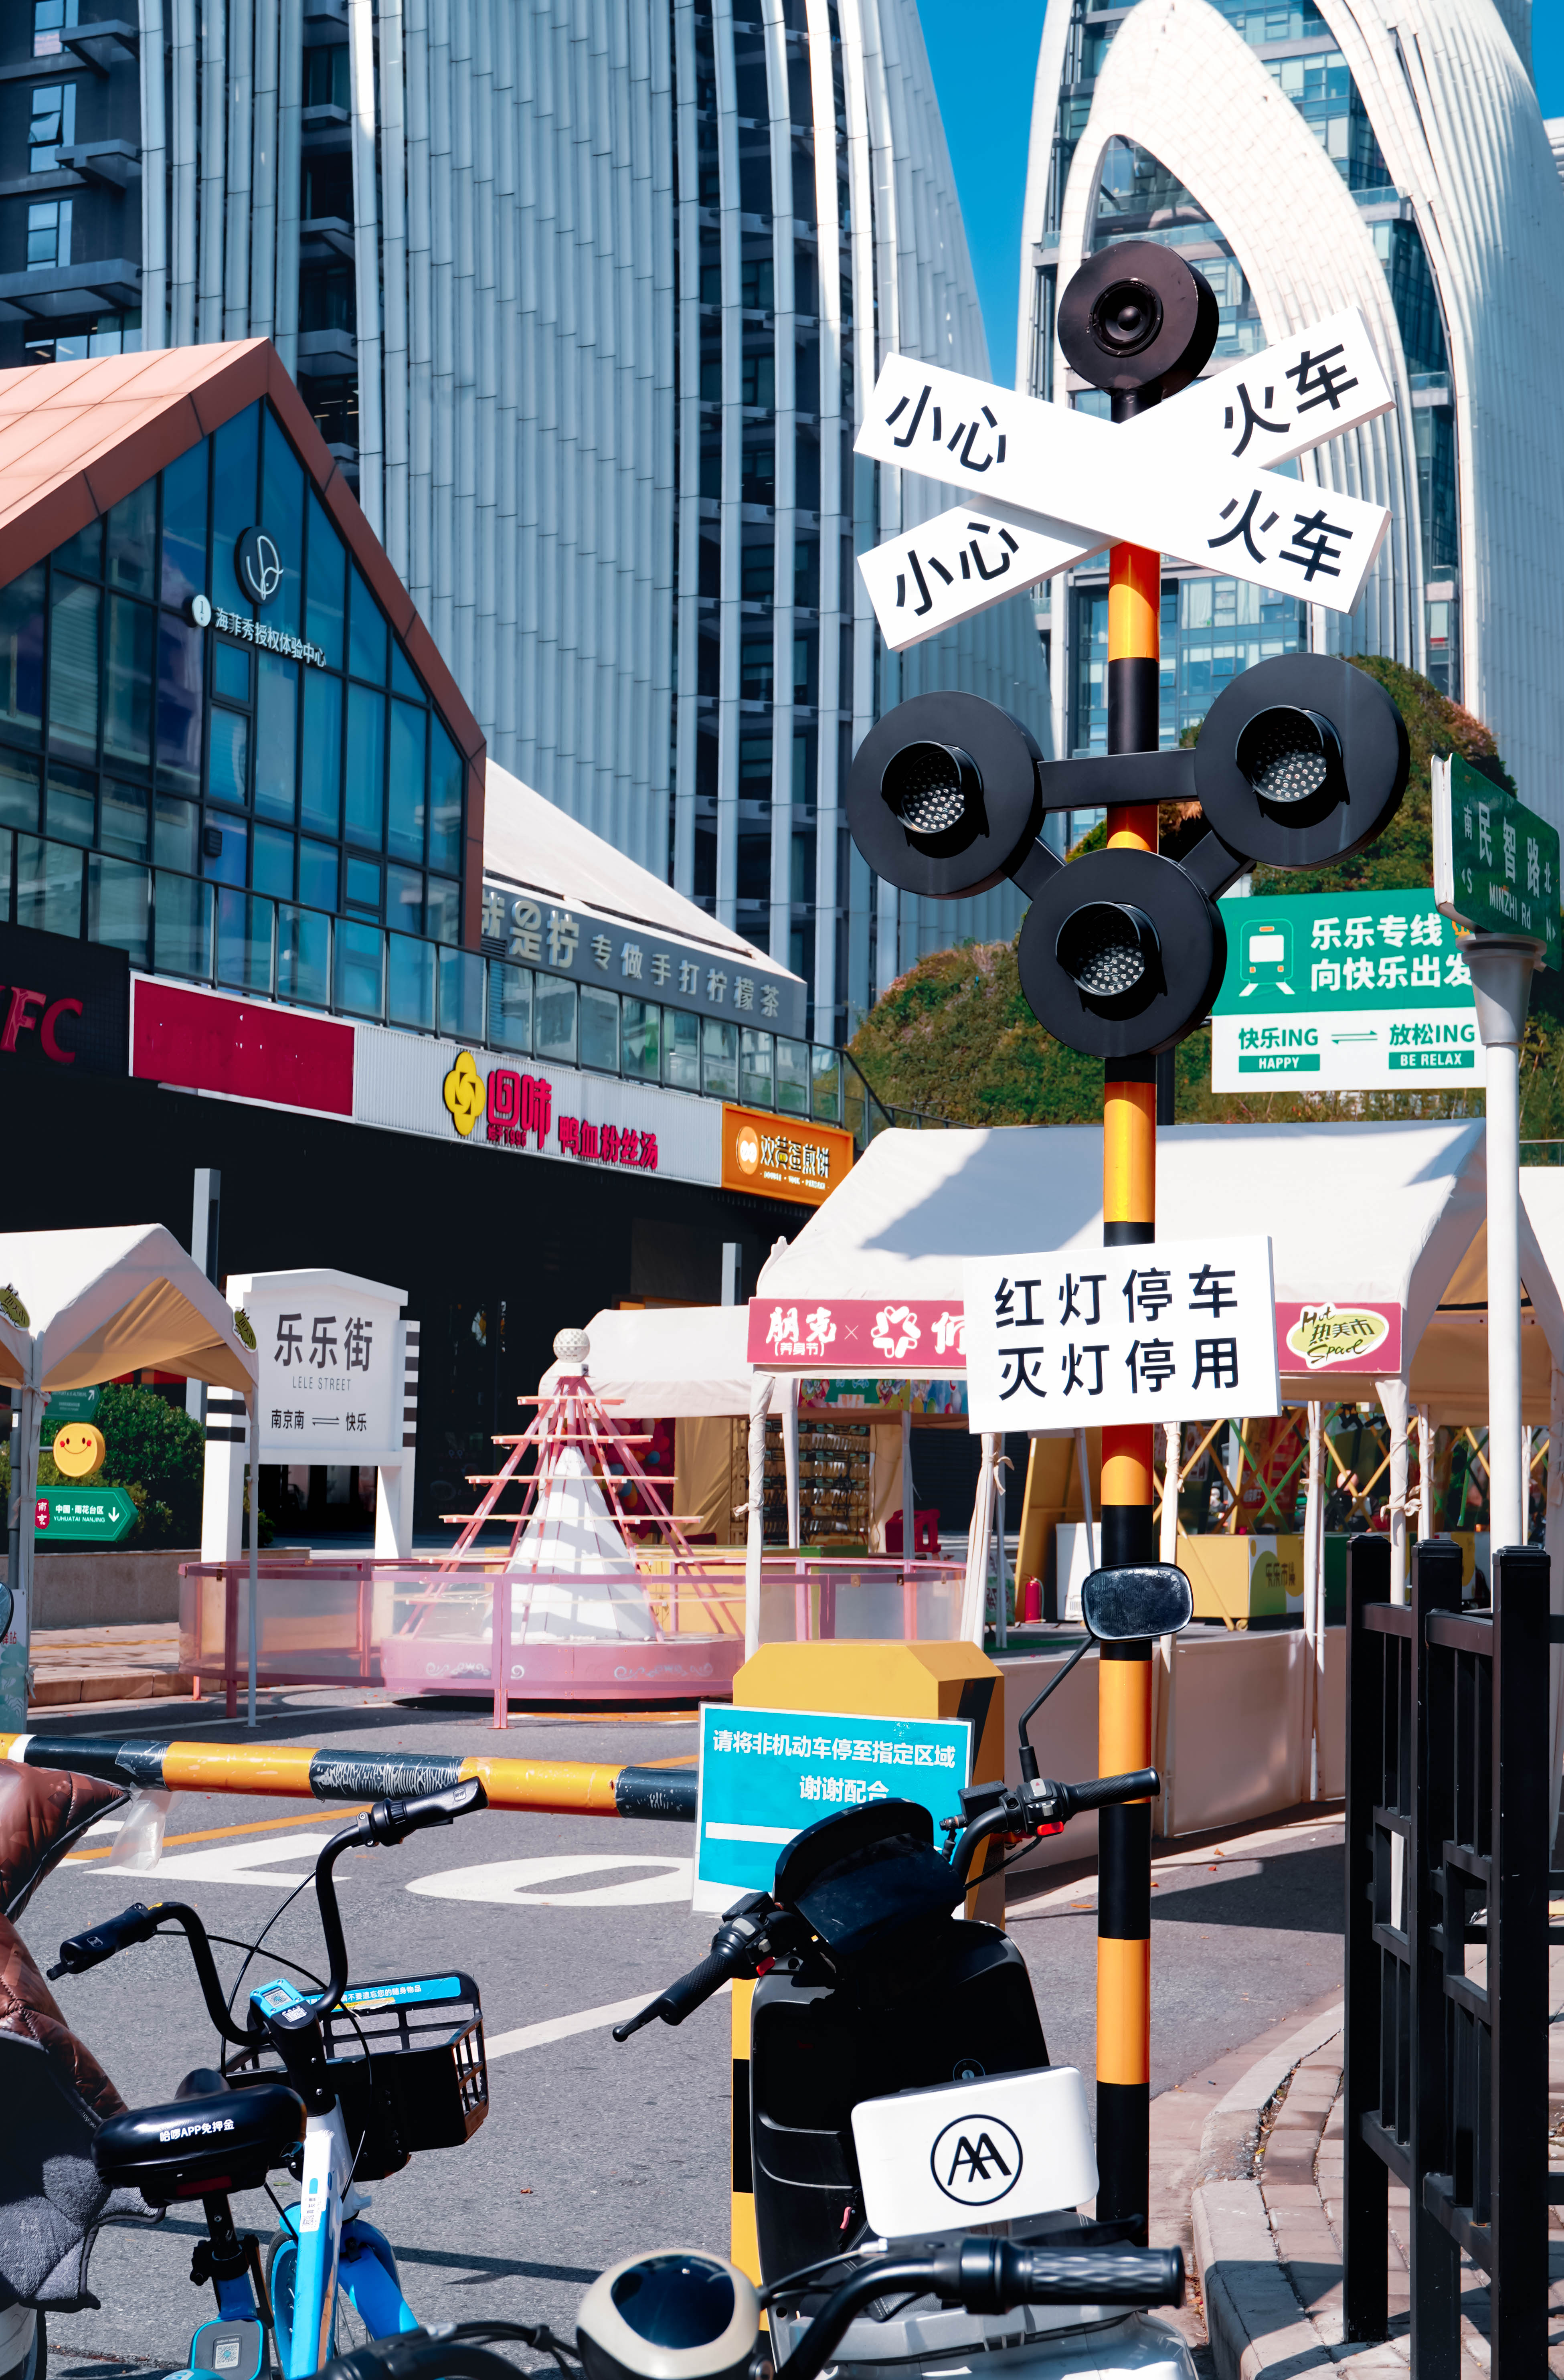
\includegraphics[width=\paperwidth,height=\paperheight]{src/Figures/Arriere_plan/Arriere_plan_Chap_6.jpg}
}

% Rectangle
\AddToShipoutPictureBG*{
  \begin{tikzpicture}[remember picture,overlay]
    \node[fill=white, opacity=0.75, text width=\paperwidth, minimum height=11cm, anchor=north] 
    at ([yshift=-2cm]current page.north) {};
  \end{tikzpicture}
}

% Source
\AddToShipoutPictureFG*{
  \AtPageLowerRight{
    \raisebox{1cm}{
      \hspace{16cm}
      
\begin{tikzpicture}
        \node[fill=white, rounded corners=5pt, inner sep=5pt, align=center] {
          \tiny{Photography: \textcolor{blue}{Dylan Moinse (2024)}}
        };
      \end{tikzpicture}
    }
  }
}

    % ___________________________________________
    % Mini Table of Contents
    \cleardoublepage
    \setcounter{tocdepth}{2}
    % Redefine local table of contents title
    \renewcommand{\localcontentsname}{Table of Contents for Chapter~6}
\localtableofcontents

% Reset section numbering
\setcounter{section}{0}

    % ___________________________________________
    % Graphical Abstract
    \newpage
\section*{Key Points of Chapter~6
    \label{chap6:graphical-abstract}
    }
    \markright{Chapter Preamble}{}

\begin{figure}[h!]\vspace*{4pt}
        \caption*{}
        \label{graphical-abstract-chap6}
        \centerline{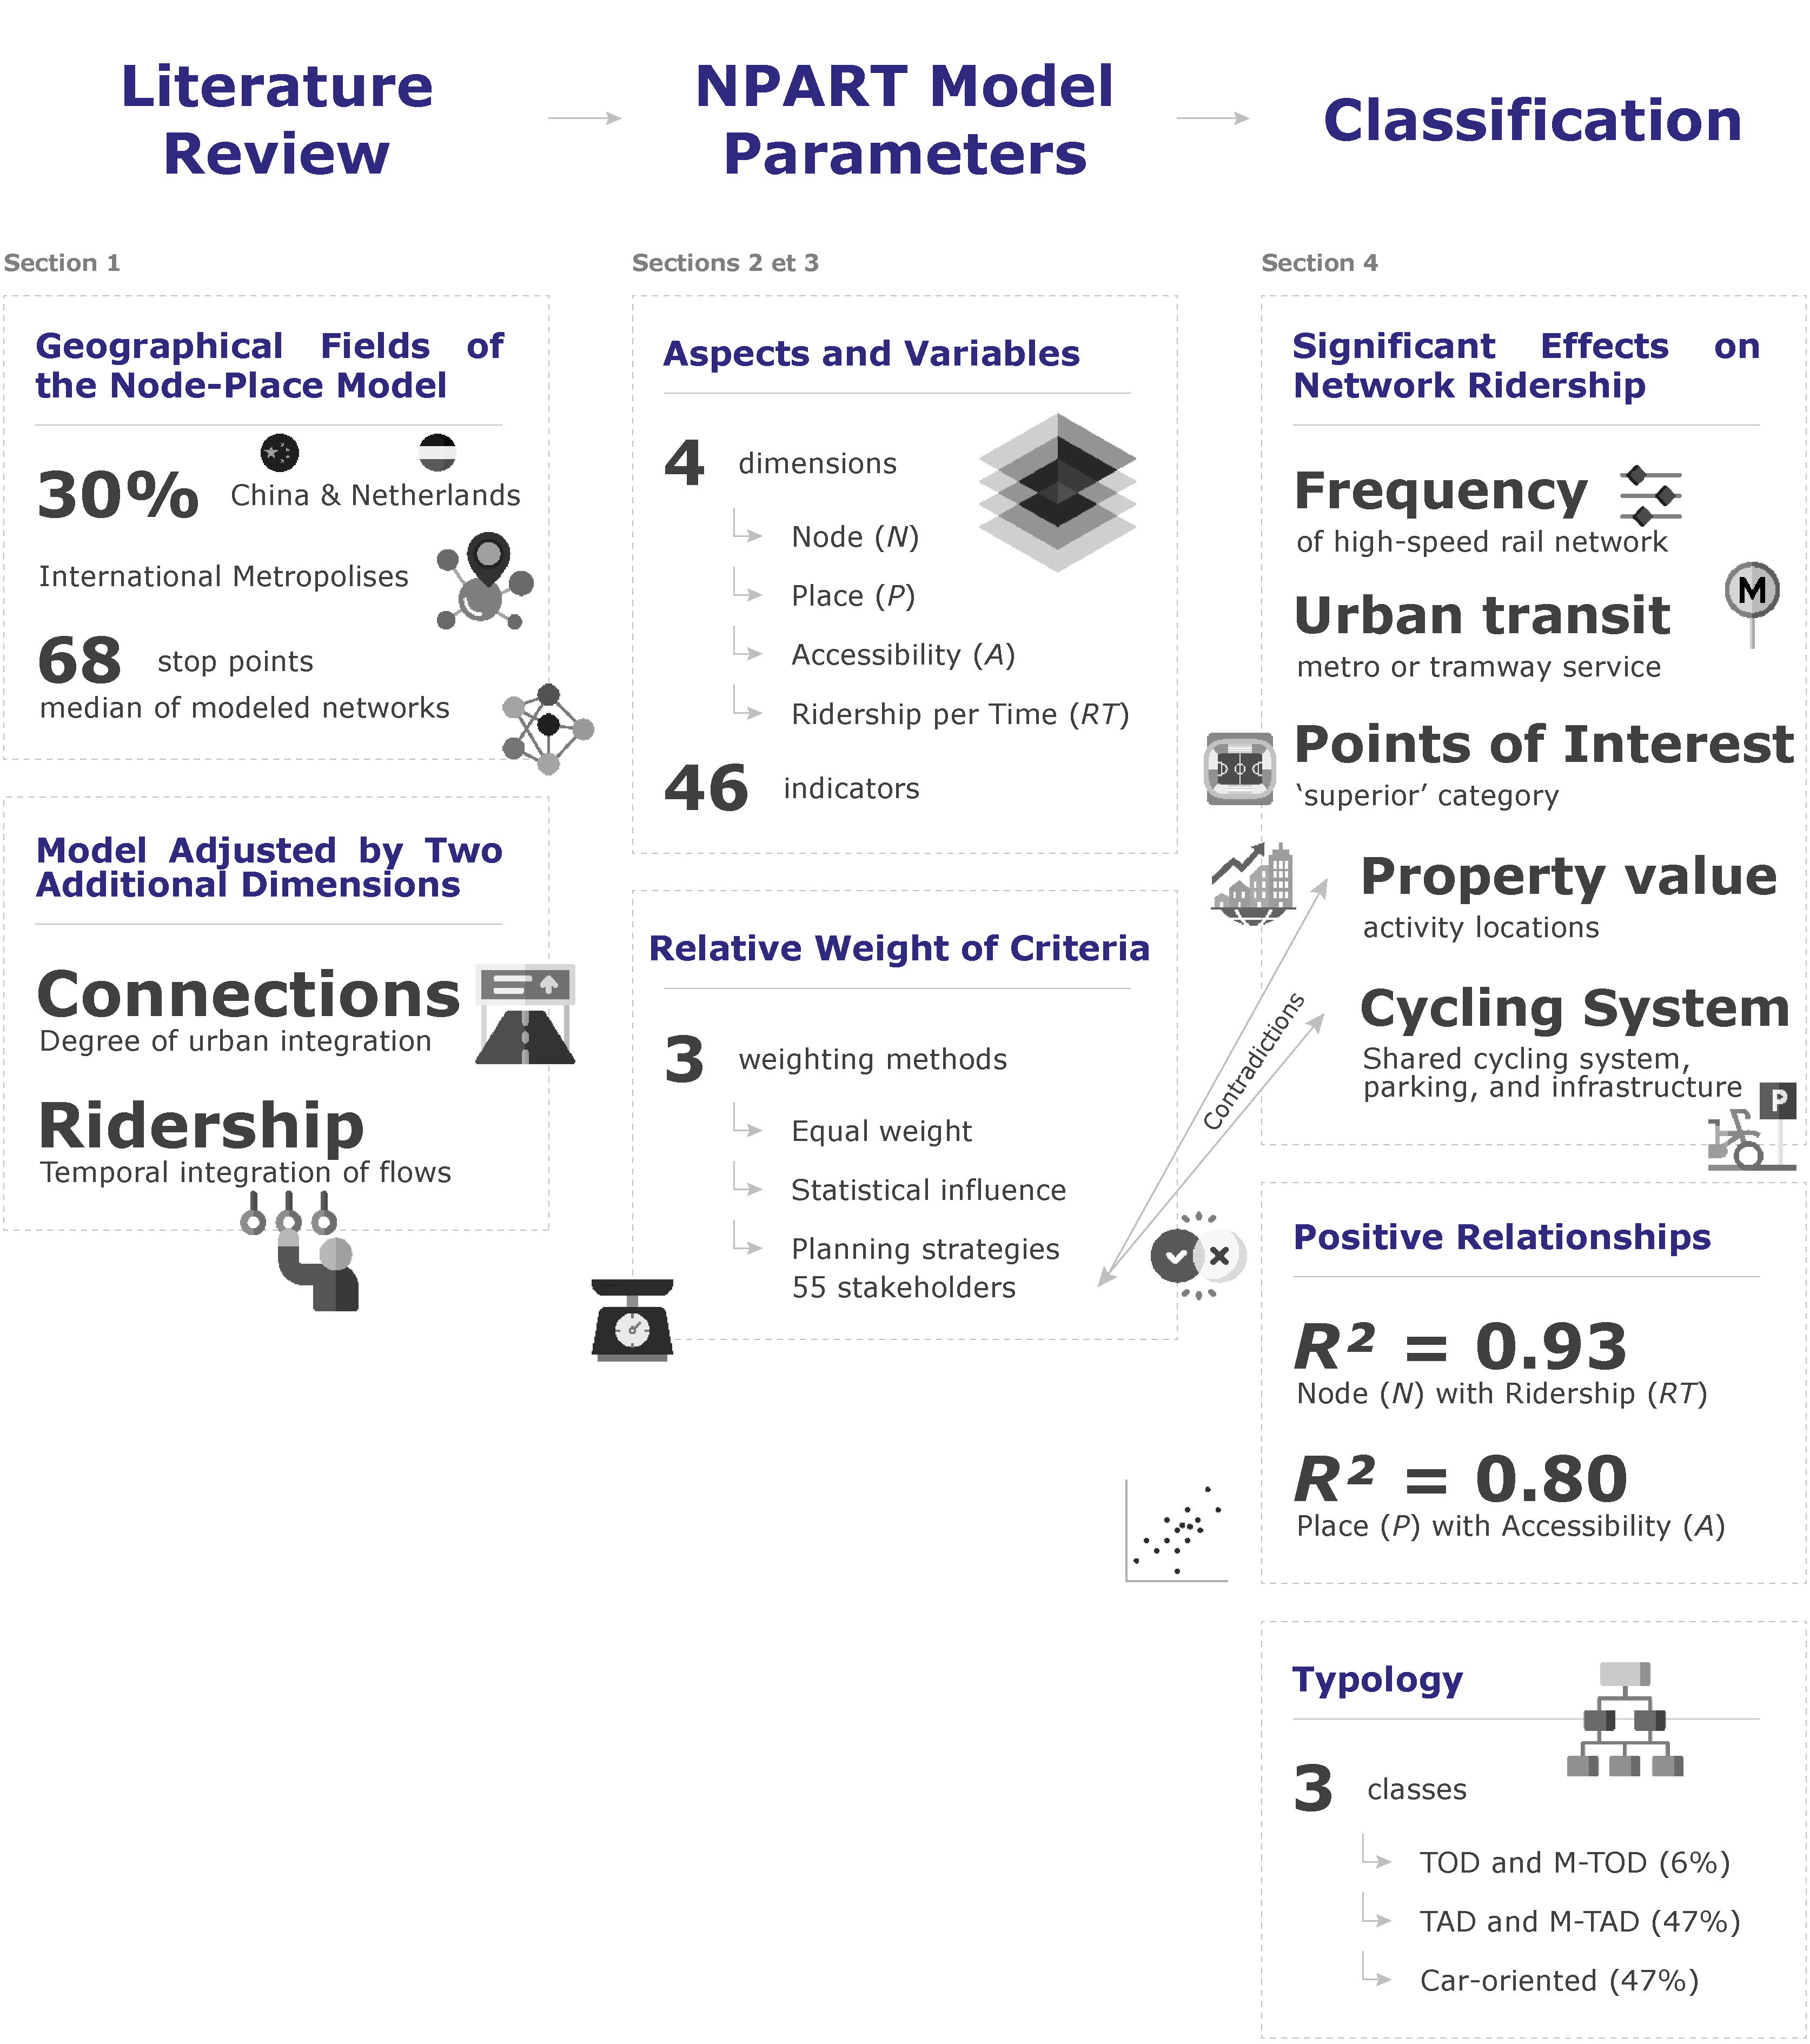
\includegraphics[width=1\columnwidth]{src/Figures/Graphical-abstract/EN_Graphical_abstract_chap6.pdf}}
        \vspace{5pt}
    \end{figure}

% ___________________________________________
% Preambule
\newpage
\begin{tcolorbox}[colback=white!5!white,
                      colframe=blue!75!blue,
                      title=
                      \bigskip
                      \center{\textbf{Preambule of Chapter~6}}
                      \\
                      \raggedright{\small{Chapter composed of \pagedifference{chap6:titre}{part3:conclusion} pages, including \pagedifference{chap6:bibliographie}{part3:conclusion} pages of bibliography}}
                      \bigskip]
\Large{\textcolor{blue}{\textbf{Abstract:}}}
    \\
    \small{
This chapter presents an in-depth analysis of the development potential of station districts in the Hauts-de-France region, based on the application of the \Commas{node-place model}. This multi-criteria analytical tool evaluates the degree of integration between public transport services and the socio-economic and urban characteristics of the surrounding territories. The model enables the mapping of development opportunities by identifying \Commas{balance} or \Commas{imbalance} relationships between these two dimensions, thus providing a basis for developing integrated \acrfull{TOD} strategies.%%Translated%%
    \\
Initially, we review the scientific literature to define the theoretical and methodological framework of this technical approach (see the \hyperref[chap6:revue-litterature-m-tod-index]{literature review on the urban model}, page~\pageref{chap6:revue-litterature-m-tod-index}). Previous research has mainly focused on metropolitan contexts, particularly in Asia and Northern Europe. However, its application in sparsely or moderately dense areas, at a regional scale like that of Hauts-de-France, remains largely underutilized, highlighting the need for a methodological adaptation to local realities. The revisited model, which we have named \acrfull{NPART} (see the \hyperref[chap6:selection-indicateurs]{model parameters} and the \hyperref[chap6:methodologie-m-tod-index]{processing of collected data}, pages~\pageref{chap6:selection-indicateurs} and~\pageref{chap6:methodologie-m-tod-index}), innovates in several ways: (i) original application in a geographically under-studied area; (ii) the addition of two dimensions focusing on the quality of public spaces and the dynamic usage of stations; (iii) a comparative approach between station districts accessible on foot and by light individual mobility; and (iv) the integration of advanced statistical techniques, such as tools from \textsl{Machine Learning}.%%Translated%%
    \\
The results of the study provide several significant contributions in the \hyperref[chap6:resultats-modele]{section presenting key results} (page~\pageref{chap6:resultats-modele}): (i) they demonstrate the relevance of the model for diagnosing opportunities for urban redevelopment, (ii) they refocus discussions on the importance of redefining geographical and methodological scales, (iii) and they highlight the potential of developing this model in France, where its application remains limited despite its potential to promote urban revitalization projects. The geostatistical analysis of \acrshort{NPART} also identified the most influential urban criteria for defining and supporting the \acrshort{TOD} concept and its variation, which we propose under the name \acrshort{M-TOD}, covering aspects such as the quality of rail service, urban development intensity, and \gls{accessibility} through proximity. A classification of train-served territories was established, distinguishing three categories: \textsl{rail-oriented} territories, territories whose activities are \textsl{adjacent} to the public transport infrastructure, and \textsl{self-centered} territories. This regional typology encourages focusing efforts on the second class, which includes half of the network's stations and shows \acrshort{TOD} potential from the pedestrian and cycling perspectives.%%Translated%%
    }
    \tcblower
\Large{\textcolor{blue}{\textbf{Keywords:}}}
    \\
    \small{
Accessibility;
Classification;
Temporal usage;
\Marque{GitHub};
Node-place model;
NPART;
Planners' perspective;
\textsl{Transit-Oriented Development} potential;
Prediction;
\textsl{Python};
Radar;
\textsl{Transit-Adjacent Development}
    }
    \end{tcolorbox}

% ___________________________________________
% 6.*.
\newpage
\needspace{1\baselineskip} % Reserve space
\addcontentsline{toc}{section}{Introduction of Chapter~6}
\sectionheader{Introduction of Chapter~6}
\section*{Introduction of Chapter~6
    \label{chap6:introduction}
    }
    \markright{Introduction of Chapter~6}{}

    % Citation
    \begin{displayquote}
\Commas{\textsl{A specific part of the academic literature on TOD focuses on identifying the development potential of transit station areas as an outcome of the interplay between transport and land use dimensions. The ‘node-place model’ is the analytical framework that is predominantly used to map the differentiated development opportunities of station(s) areas(s). The assumption underlying most NPM studies is that a systematic inventory of both characteristics for a particular set of stations (along a corridor or within a region), provides useful knowledge that can subsequently inform evidence-based policy discussions, decision making processes and planning practices.} [\dots] \textsl{The model furthermore allows to benchmark and compare stations and draft more targeted TOD strategies for groups of stations}. [\dots] \textsl{Finally, the 3000 m classification is the least similar to the other three. Not only is there a significant difference with the 800 m classification, there is also a pronounced difference with the 1200 m classification. These results suggest that analyses focused on bicycle-TOD may reveal radically different typology outcomes than the typically walking-induced types of TOD in which typically smaller CAs are used.}}

\textcolor{blue}{Freke} \textcolor{blue}{\textcite[50, 83]{caset_planning_2019}}\index{Caset, Freke|pagebf}. \textsl{Planning for Nodes, Places, and People: a Strategic Railway Station Development Tool for Flanders}. Thèse de doctorat en Géographie. Université de Gand, Université libre de Bruxelles, 198~p. \url{http://hdl.handle.net/1854/LU-8637955}
    \end{displayquote}

% Introduction
\lettrine[lines=3, findent=8pt, nindent=0pt]{\lettrinefont T}{he} \acrfull{NPM} constitutes an analytical and operational framework within the field of \acrfull{TOD} research. It is based on the assumption that public transport infrastructures, when integrated into their urban environment, can promote forms of compact, accessible, and economically dynamic development. This perspective encourages considering train stations as local development catalysts, depending on their connectivity and the intensity of activities organized around them. This analytical framework is based on two fundamental axes: the \textsl{node} index and the \textsl{place} index, whose \Commas{balance} ensures the integrated development of station neighborhoods \textcolor{blue}{\autocite[202]{bertolini_spatial_1999}}\index{Bertolini, Luca|pagebf}. This systemic approach allows for understanding the complexity of interactions between networks and territories, in other words, the urban insertion of train stations using functional and structural indicators \textcolor{blue}{\autocite[25]{albertelli_variations_2024}}\index{Albertelli, Marion|pagebf}, based on a system of quantitative evaluation \textcolor{blue}{\autocite[47]{chorus_application_2011}}\index{Chorus, Paul|pagebf}\index{Bertolini, Luca|pagebf}.%%Translated%%

% Literature gaps
The choice of such an analytical tool is explained by its recent, yet recognized, ability to assess the relationship between the intensity of public transport supply and that of the urban system. In this respect, we follow the recommendations made by \textcolor{blue}{\textcite[111]{nigro_land_2019}}\index{Nigro, Antonio|pagebf}\index{Bertolini, Luca|pagebf}\index{Moccia, Francesco Domenico|pagebf}, who highlight the limitations of previous conceptualizations of \acrshort{NPM}, particularly the exclusion of the role of feeder modes and, consequently, the level of connection of station catchment areas. While existing models have primarily focused on walkability-friendly connections, the role of the \gls{bicycle} and \gls{micromobility} remains largely underexplored within the framework of \acrshort{NPM} \textcolor{blue}{\autocite[2]{zhang_make_2023}}\index{Zhang, Mengyuan|pagebf}\index{Lee, Jinwoo Brian|pagebf}. As a result, most approaches are limited to the analysis of buffer zones of 800 meters, rendering these models partially outdated according to \textcolor{blue}{\textcite[12]{olaru_place_2019}}\index{Olaru, Doina|pagebf}\index{Moncrieff, Simon|pagebf}\index{McCarney, Gary|pagebf}\index{Sun, Yuchao|pagebf}\index{Reed, Tristan|pagebf}\index{Pattison, Cate|pagebf}\index{Smith, Brett|pagebf}\index{Biermann, Sharon|pagebf}. As illustrated by \hyperref[fig-chap6:revue-tailles-aires]{Figure~\ref{fig-chap6:revue-tailles-aires}} (page~\pageref{fig-chap6:revue-tailles-aires}), the station neighborhoods defined in various \acrshort{NPM} models generally have spatial boundaries not exceeding an average radius of one kilometer. This approach leads to a very limited, or even almost nonexistent, consideration of modes of transportation such as cycling and micromobility. The figure highlights the predominance of very small micro-geographical perimeters, perceptible through the thicknesses of the smallest circles represented.%%Translated%%

% Figure Literature station neighborhood sizes
\begin{figure}[h!]\vspace*{4pt}
    \caption{Review of station neighborhood sizes defined within the framework of node-place models.}
    \label{fig-chap6:revue-tailles-aires}
    \centerline{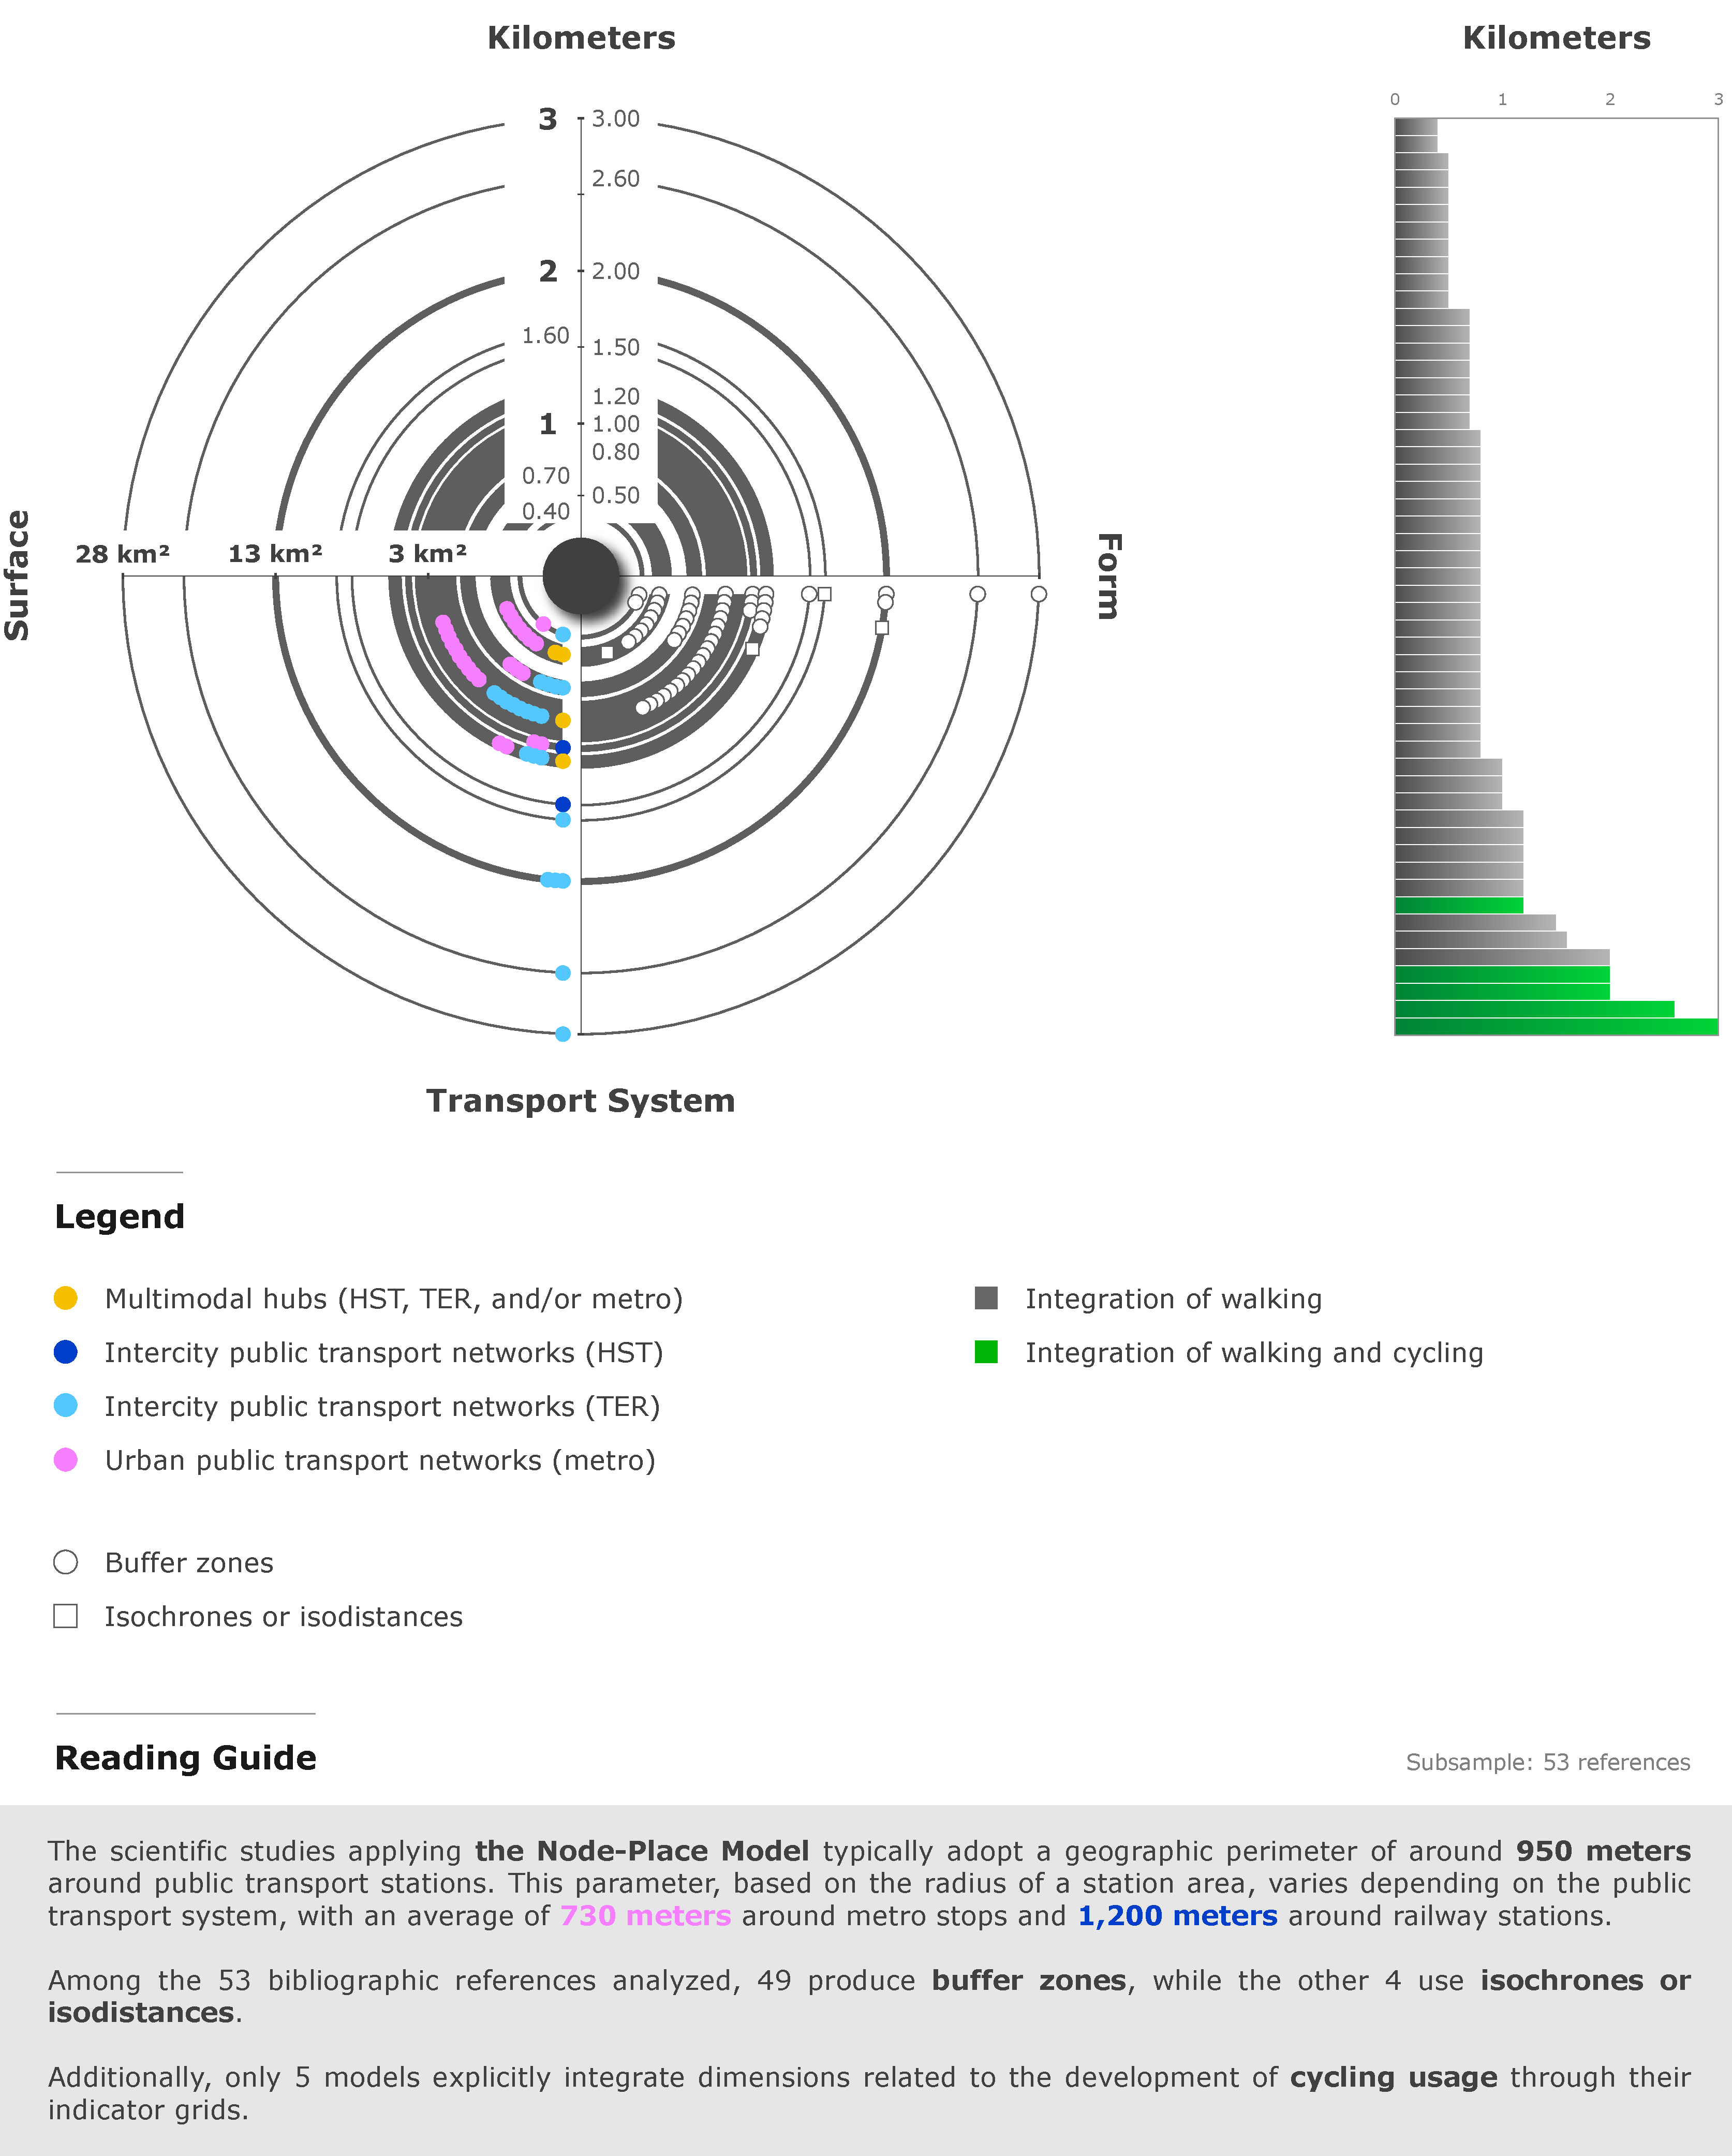
\includegraphics[width=1\columnwidth]{src/Figures/Chap-6/EN_NPART_Distances_quartiers_gare.pdf}}
    \vspace{5pt}
    \begin{flushright}\scriptsize{
    Realization: \textcolor{blue}{Dylan Moinse (2024)}
    \\
    Authors: \acrshort{NPART} Research Project
    }\end{flushright}
\end{figure}

% General Questioning
This chapter extends the work initiated by applying the \acrshort{NPM} to station neighborhoods in the Hauts-de-France region. The main objective is to offer an advanced understanding of the urban development potential in this study area, while incorporating our research questions on the integration of light individual mobility. We are thus interested in the development potential of the studied station neighborhoods. The main sub-objectives guiding this analysis are as follows:
\begin{customitemize}
    \item \textsl{Spatio-temporal contextualization}. Integrate an intermodal perspective by assessing the contribution of light individual mobility while considering urban rhythms and comparing it to pedestrian accessibility;
    \item \textsl{Model calibration}. Enrich the existing model by incorporating new relevant dimensions to broaden the concept of urban planning;
    \item \textsl{Geographical scale}. Apply the revised model to the Hauts-de-France region, marked by a diversity of urban forms;
    \item \textsl{Descriptive statistics}. Analyze the influence of different variables on station attractiveness;
    \item \textsl{Classification of stations and their surroundings}. Define and describe the interactions of nodes and their immediate surroundings to establish a typology of stations;
    \item \textsl{Reproducibility and automation}. Develop a methodological framework that is both reproducible and automated for the collection and analysis of geographic data, ensuring the adoption of the modeling approach.
\end{customitemize}%%Translated%%

% Outline Announcement 1
We begin this chapter with a presentation of the literature review on the \acrshort{NPM}, aiming to highlight the different approaches adopted to assess the development potential of station neighborhoods (\hyperref[chap6:revue-litterature-m-tod-index]{Section~\ref{chap6:revue-litterature-m-tod-index}}, page~\pageref{chap6:revue-litterature-m-tod-index}). This critical analysis primarily serves to identify the contributions and limitations of existing work. Initially, we positioned the model within a broader conceptual framework (\hyperref[chap6:litterature-concept]{Subsection~1.1}, page~\pageref{chap6:litterature-concept}), before providing an overview of the identified studies to trace the model's evolution throughout the research (\hyperref[chap6:litterature-etat-art]{Subsection~1.2}, page~\pageref{chap6:litterature-etat-art}).%%Translated%%

% Outline Announcement 2
Based on the weaknesses identified in the literature review, the parameters selected for our modeling are introduced (\hyperref[chap6:selection-indicateurs]{Section~\ref{chap6:selection-indicateurs}}, page~\pageref{chap6:selection-indicateurs}). This section details the various dimensions and indicators chosen for the implementation of our \acrfull{NPART} model. The analysis is structured around the four main components of the model, encompassing a total of 46 indicators. These dimensions include the node (\hyperref[chap6:methodologie-indicateurs-node]{Subsection~2.1}, page~\pageref{chap6:methodologie-indicateurs-node}), the place (\hyperref[chap6:methodologie-indicateurs-place]{Subsection~2.2}, page~\pageref{chap6:methodologie-indicateurs-place}), local accessibility (\hyperref[chap6:methodologie-indicateurs-accessibility]{Subsection~2.3}, page~\pageref{chap6:methodologie-indicateurs-accessibility}), and frequency (\hyperref[chap6:methodologie-indicateurs-frequentation]{Subsection~2.4}, page~\pageref{chap6:methodologie-indicateurs-frequentation}).%%Translated%%

% Outline Announcement 3
The third section is dedicated to the collection and processing of geostatistical data required for the implementation of the urban model (\hyperref[chap6:methodologie-m-tod-index]{Section~\ref{chap6:methodologie-m-tod-index}}, page~\pageref{chap6:methodologie-m-tod-index}). It presents the various techniques used for extracting and validating the collected data (\hyperref[chap6:methodologie-statistiques]{Subsection~3.1}, page~\pageref{chap6:methodologie-statistiques}), then discusses segmentation and classification methods (\hyperref[chap6:methodologie-statistiques-clusterisation-classification]{Subsection~3.2}, page~\pageref{chap6:methodologie-statistiques-clusterisation-classification}), as well as approaches for weighting the indicators (\hyperref[chap6:methodologie-ponderation-indicateurs]{Subsection~3.3}, page~\pageref{chap6:methodologie-ponderation-indicateurs}).%%Translated%%

% Outline Announcement 4
Before concluding this chapter, we engage in a discussion of the statistical results obtained from a given situation (\hyperref[chap6:resultats-modele]{Section~\ref{chap6:resultats-modele}}, page~\pageref{chap6:resultats-modele}). By analyzing the relative influence of each model parameter, we were able to refine the definitions of the \acrshort{TOD} and \acrshort{M-TOD} models in their essence (\hyperref[chap6:results-influence-indicateurs]{Subsection~4.1}, page~\pageref{chap6:results-influence-indicateurs}). At the regional scale, the modeling allowed us to provide an overview of stations and their surroundings, classifying them into areas considered as \Commas{accessible} or \Commas{dependent} (\hyperref[chap6:results-caracterisation-gares]{Subsection~4.2}, page~\pageref{chap6:results-caracterisation-gares}). Finally, these results were synthesized in the form of a classification, enriched with a description of the labels assigned to each category (\hyperref[chap6:results-classification-gares]{Subsection~4.3}, page~\pageref{chap6:results-classification-gares}).%%Translated%%

% Outline Announcement 5
In conclusion, we summarize the key points of this chapter, which is built around the conceptualization and application of the \acrshort{NPART} model. These analyses provide insight into the diagnosis of the current and potential development of stations and their surroundings, both at the pedestrian and cycling scales (\hyperref[chap6:conclusion]{Chapter~6 conclusion}, page~\pageref{chap6:conclusion}).%%Translated%%

    % ___________________________________________
    % 6.1.
    \newpage
    \needspace{1\baselineskip} % Reserve space
    \sectionheader{Literature review of the \Commas{node-place model}}
\section{Assessment and Classification of the Territorial Development Potential around Train Stations through the \Commas{Node-Place Model}
    \label{chap6:revue-litterature-m-tod-index}
    }

    % Objectives of the NP
The \acrfull{NPM}, whose theoretical framework was presented by \textcolor{blue}{Luca} \textcolor{blue}{\textcite[343]{bertolini_nodes_1996}}\index{Bertolini, Luca|pagebf} at the Faculty of Geography at Utrecht University, is a tool designed to measure the intensity of public transport supply associated with a node within a network, in relation to the activities of a given territory. The \acrshort{NPM} is presented as a multicriteria analysis model, evaluating redevelopment opportunities while integrating the concept of \Commas{balance}, considered not only at the scale of a train station district but also in the broader perspective of the public transport network, as illustrated by \textcolor{blue}{Luca} \textcolor{blue}{\textcite[206]{bertolini_spatial_1999}}\index{Bertolini, Luca|pagebf} in its application to the metropolitan areas of Amsterdam and Utrecht. This model is based on the principle that a single indicator is insufficient to capture territorial complexity. Therefore, this methodological approach requires consideration of multiple dimensions \textcolor{blue}{\autocite[5]{arliani_measuring_2023}}\index{Arliani, Vani|pagebf}\index{Sjafruddin, Ade|pagebf}\index{Santoso, Idwan|pagebf}\index{Winarso, Haryo|pagebf}. According to \textcolor{blue}{Luca} \textcolor{blue}{\textcite[200]{bertolini_spatial_1999}}\index{Bertolini, Luca|pagebf}, the aim of the \acrshort{NPM} is to promote \Commas{centralized decentralisation}, allowing the study of urban environment characteristics around public transport stations to foster a territorial design of the \acrfull{TOD} type \textcolor{blue}{\autocite[55]{kamruzzaman_advance_2014}}\index{Kamruzzaman, Md.|pagebf}\index{Baker, Douglas|pagebf}\index{Washington, Simon|pagebf}\index{Turrell, Gavin|pagebf}, and more specifically, the applicability of this urban strategy \textcolor{blue}{\autocites[516-517]{filion_smart_2007}[97]{curtis_delivering_2012}}.%%Translated%%

    % Outline of the plan
In this section, we aim to reposition this model within a conceptual, methodological, chronological, and geographical analysis, questioning the value of a geostatistical approach of this type and synthesizing its various contributions in relation to the \acrshort{TOD} and its recent developments. We will first focus on the conceptual and methodological framework underlying the model's objective of examining nodes and their environments (see the \hyperref[chap6:litterature-concept]{section on the literature review of this approach}, page~\pageref{chap6:litterature-concept}). This will be followed by an overview of the various existing contributions, taking into account geographical contexts and the interpretations attributed to this highly flexible model. The aim is thus to identify, in connection with our project, the gaps in the current literature concerning this model and its relevance to answering our research questions.%%Translated%%

    % 6.1.1.
    \needspace{1\baselineskip} % Reserve space
\subsection{A Methodological Framework to Characterize the Coordination between Public Transport Services and Territorial Dynamics
    \label{chap6:litterature-concept}
    }

   % Node and place indices
The methodology adopted to analyze the train station and station district pair relies on the characterization of the node (\textsl{node}) and its surrounding territory (\textsl{place}), using two synthetic indicators \textcolor{blue}{\autocites[343]{bertolini_nodes_1996}[199]{bertolini_spatial_1999}}\index{Bertolini, Luca|pagebf}. The combination of these two indicators allows for the exploration of the still underexplored multiscalar interaction between public transport network nodes (\textsl{nodes of networks}) and urban places (\textsl{places in the city}), according to \textcolor{blue}{Luca} \textcolor{blue}{\textcite[344]{bertolini_nodes_1996}}\index{Bertolini, Luca|pagebf}. This model is primarily an \Commas{\textsl{analytical tool to identify the potential for public transport-oriented urban-regional development}}\footnote{~
    \Commas{[\dots] \textsl{an analytical tool to help identify the potential for public transport-oriented urban-regional development.}} \textcolor{blue}{\autocite[199-201]{bertolini_spatial_1999}}\index{Bertolini, Luca|pagebf}.
} with a node index designed to examine the \Commas{potential for physical human interaction} and a place index designed as the \Commas{degree of actual realization of this potential}, to use the words of \textcolor{blue}{Luca} \textcolor{blue}{\textcite[199-201]{bertolini_spatial_1999}}\index{Bertolini, Luca|pagebf}. Based on a feedback model, this analytical framework examines how land use reflects and benefits from the advantages of public transport, and \textsl{vice versa} \textcolor{blue}{\autocite[47]{chorus_application_2011}}\index{Chorus, Paul|pagebf}\index{Bertolini, Luca|pagebf}. The \Commas{pair} node and place is based on the idea that improving public transport supply creates conditions conducive to urban development, which in turn intensifies the demand for mobility, thereby promoting the development of the mobility system \textcolor{blue}{\autocite[47]{chorus_application_2011}}\index{Chorus, Paul|pagebf}\index{Bertolini, Luca|pagebf}. Exploring the interrelations between various factors can then support public policies by promoting \acrshort{TOD} and proposing a classification that would help direct investments more effectively in each type of train station district.%%Translated%%

    % 6.1.1.1.
    \needspace{1\baselineskip} % Reserve space
\subsubsection*{An Analytical Tool for Accessibility \textsl{by} and \textsl{around} Public Transport Stations
    \label{chap6:litterature-concept-accessibilite}
    }

    % NP Accessibility
The \acrshort{NPM} model is fundamentally designed to understand the concept of accessibility, within which it seeks to examine the joint effects of transport networks (\textsl{network science}) and the characteristics of the urban environment (\textsl{spatial science}), an approach that resonates with the perspectives outlined by \textcolor{blue}{\textcite[300]{ducruet_spatial_2014}}\index{Ducruet, César|pagebf}\index{Beauguitte, Laurent|pagebf}. Indeed, the model mobilizes the concept of accessibility based on the assumption that an accessible node also requires an accessible place, and vice versa \textcolor{blue}{\autocite[203]{bertolini_spatial_1999}}\index{Bertolini, Luca|pagebf}. This approach strategically positions the public transport station at the heart of the network to which it belongs, emphasizing the mobility opportunities and accessible prospects it offers \textcolor{blue}{\autocite[3]{amini_pishro_node_2022}}\index{Amini Pishro, Ahad|pagebf}\index{Yang, Qihong|pagebf}\index{Zhang, Shiquan|pagebf}\index{Amini Pishro, Mojdeh|pagebf}\index{Zhang, Zhengrui|pagebf}\index{Zhao, Yana|pagebf}\index{Postel, Victor|pagebf}\index{Huang, Dengshi|pagebf}\index{Li, WeiYu|pagebf}. This vision aligns with the paradigm shift driven by \acrshort{TOD} \textcolor{blue}{\autocite[75]{banister_sustainable_2008}}\index{Banister, David|pagebf}, which promotes a shift from mobility-centered planning (\textsl{planning for mobility}) to accessibility-centered planning (\textsl{planning for accessibility}), within which the model is situated \textcolor{blue}{\autocite[496]{caset_measuring_2018}}\index{Caset, Freke|pagebf}\index{Vale, David~S.|pagebf}\index{Viana, Cláudia~M.|pagebf}. It should be noted that the model specifically focuses on the concept of \Commas{relative accessibility}, as defined by \textcolor{blue}{\textcite[27]{dalvi_measurement_1976}}\index{Dalvi,~M.~Q.|pagebf}\index{Martin,~K.~M.|pagebf}, which focuses on \Commas{[\dots] \textsl{not on the change in the absolute accessibility of a territory, but rather on the change in its relative position compared to other territories on an accessibility scale}}\footnote{~
    \Commas{\textsl{What is, however, more interesting to note is not the change in the absolute accessibility of different areas when the value of \(\beta\) changes, but the change in their relative position, vis-à-vis each other on the accessibility scale} [\dots]} \textcolor{blue}{\autocite[27]{dalvi_measurement_1976}}\index{Dalvi,~M.~Q.|pagebf}\index{Martin,~K.~M.|pagebf}.
}. This comparative perspective on accessibility is also supported by \textcolor{blue}{\textcite[521]{caset_measuring_2018}}\index{Caset, Freke|pagebf}\index{Vale, David~S.|pagebf}\index{Viana, Cláudia~M.|pagebf}, who argue that the \acrshort{NPM} model highlights the development possibilities of stations in terms of urbanism and mobility, effectively linking transport networks with territorial dynamics. In doing so, the \acrshort{NPM} proves to be a powerful analytical tool for guiding public policies and urban planning strategies, placing accessibility at the core of transport infrastructure planning and urban development.%%Translated%%

    % TOD Index Difference
Accessibility plays a central role in the design of the \acrshort{NPM}, as it aims to shed light on the links between the connectivity of a space as a \textsl{node} and its characteristics as a \textsl{place}. The choice of such a tool calls for a distinction from another measure of the \acrshort{TOD}, namely the \acrshort{TOD} Index\footnote{~
    The \acrshort{TOD} Index was proposed by \textcolor{blue}{\textcite[9]{evans_transit-oriented_2007}}\index{Evans, James|pagebf}\index{Pratt, Richard|pagebf}\index{Stryker, Andrew|pagebf}\index{Kuzmyak,~J.|pagebf} to measure the \acrshort{TOD} potential (\textsl{TOD-ness}). This indicator is proposed as a tool to characterize the degree to which a territory or project adheres to the principles of the development concept. It was designed to capture the key elements of what is called a \Commas{successful} development \textcolor{blue}{\autocite[97]{evans_transit-oriented_2007}}\index{Evans, James|pagebf}\index{Pratt, Richard|pagebf}\index{Stryker, Andrew|pagebf}\index{Kuzmyak,~J.|pagebf} to measure the \acrshort{TOD} potential (\textsl{TOD-ness}).
}, an indicator designed to assess the quality of a district in terms of access to public transport services and urban development. In contrast to the \acrshort{NPM}, which is more analytical, the \textsl{TOD Index} seeks to quantify the extent to which a territory adheres to the principles of \acrshort{TOD} \textcolor{blue}{\autocite[3]{pezeshknejad_evaluating_2020}}\index{Pezeshknejad, Parsa|pagebf}\index{Monajem, Saeed|pagebf}\index{Mozafari, Hamid|pagebf}. According to \textcolor{blue}{\textcite[96]{singh_measuring_2017}}\index{Singh, Yamini Jain|pagebf}\index{Lukman, Azhari|pagebf}\index{Flacke, Johannes|pagebf}\index{Zuidgeest, Mark|pagebf}\index{Maarseveen, Martin van|pagebf}, this indicator tends to \textsl{measure} the \acrshort{TOD} potential \textsl{before} the introduction of the network in an area, while the \acrshort{NPM} focuses on the \textsl{evaluation} of train station districts \textsl{after} the deployment of public transport systems. In this regard, the \acrshort{TOD} index is more concerned with measuring the potential (\textsl{TOD-ness}) of an area to comply with the principles of the development concept, regardless of the actual presence of a transport station, in order to establish an index, rather than a typology, which is the goal of the \acrshort{NPM} \textcolor{blue}{\autocite[97, 107]{evans_transit-oriented_2007}}\index{Evans, James|pagebf}\index{Pratt, Richard|pagebf}\index{Stryker, Andrew|pagebf}\index{Kuzmyak,~J.|pagebf}.%%Translated%%

    % 6.1.1.2.
    \needspace{1\baselineskip} % Reserve space
\subsubsection*{Building a Typology of Train Stations and Surrounding Spaces
    \label{chap6:litterature-concept-typologie}
    }

    % NP Typology
The analytical framework of the \acrshort{NPM} essentially relies on the establishment of a typology of nodes, centered around the development of a spatial index designed to assess urban development levels and mobility systems in a region. The creation of a typology, based on the functional characteristics of territories \textcolor{blue}{\autocite[2]{amini_pishro_node_2022}}\index{Amini Pishro, Ahad|pagebf}\index{Yang, Qihong|pagebf}\index{Zhang, Shiquan|pagebf}\index{Amini Pishro, Mojdeh|pagebf}\index{Zhang, Zhengrui|pagebf}\index{Zhao, Yana|pagebf}\index{Postel, Victor|pagebf}\index{Huang, Dengshi|pagebf}\index{Li, WeiYu|pagebf}, follows the main objectives of public transport-oriented planning \textcolor{blue}{\autocite[1]{motieyan_development_2018}}\index{Motieyan, Hamid|pagebf}\index{Mesgari, Mohammad Saadi|pagebf}, highlighting a concern already raised by \textcolor{blue}{Peter} \textcolor{blue}{\textcite[57]{calthorpe_next_1993}}\index{Calthorpe, Peter|pagebf}. In his foundational work, he distinguishes between \Commas{urban} train station districts (\textsl{Urban TOD}) and \Commas{neighborhood} train station districts (\textsl{Neighborhood TOD}). The classification exercise proposed by the model proves to be an effective tool for identifying and addressing the barriers to the implementation of \acrshort{TOD} \textcolor{blue}{\autocite[55]{kamruzzaman_advance_2014}}\index{Kamruzzaman, Md.|pagebf}\index{Baker, Douglas|pagebf}\index{Washington, Simon|pagebf}\index{Turrell, Gavin|pagebf}. Furthermore, the typology of stations by class simplifies the understanding of territorial configurations, facilitating comparisons and the formulation of cross-cutting strategies that benefit planners, transport managers, and stakeholders, both public and private, involved in urban production \textcolor{blue}{\autocite[55]{kamruzzaman_advance_2014}}\index{Kamruzzaman, Md.|pagebf}\index{Baker, Douglas|pagebf}\index{Washington, Simon|pagebf}\index{Turrell, Gavin|pagebf}. The growing interest in developing \Commas{normative typologies of \acrshort{TOD}} of nodes reflects a desire to provide public policies with a tool capable of informing or guiding regional planning \textcolor{blue}{\autocite[307]{higgins_forty_2016}}\index{Higgins, Christopher~D.|pagebf}\index{Kanaroglou, Pavlos~S.|pagebf}. This typology aims to evaluate a set of train station districts at the regional level, enabling comparisons between stations that do not present the same territorial development potential or the same needs in terms of intervention strategies \textcolor{blue}{\autocite[2]{iau_articulation_2017}}\index{IAU@\textsl{IAU}|pagebf}.%%Translated%%

    % Comparison with other models: 4 steps
\acrshort{TOD} districts, which manifest in various forms, require a practical tool capable of capturing the specific characteristics of each case and allowing comparisons between different entities, in order to formulate personalized recommendations to achieve the desired form, as made possible by the \acrshort{NPM} model \textcolor{blue}{\autocite[270]{li_transit_2019}}\index{Li, Zekun|pagebf}\index{Han, Zixuan|pagebf}\index{Xin, Jing|pagebf}\index{Luo, Xin|pagebf}\index{Su, Shiliang|pagebf}\index{Weng, Min|pagebf}. This model proves to be the most commonly used approach in \acrshort{TOD} studies for classifying train station districts through quantitative methods \textcolor{blue}{\autocites[3]{arliani_measuring_2023}[2]{caset_planning_2019}[1]{caset_integrating_2020}[2]{dou_integrating_2021}[113]{ibraeva_transit-oriented_2020}[270]{li_transit_2019}}\index{Arliani, Vani|pagebf}\index{Sjafruddin, Ade|pagebf}\index{Santoso, Idwan|pagebf}\index{Winarso, Haryo|pagebf}\index{Caset, Freke|pagebf}\index{Blainey, Simon|pagebf}\index{Derudder, Ben|pagebf}\index{Boussauw, Kobe|pagebf}\index{Witlox, Frank|pagebf}\index{Dou, Mingxuan|pagebf}\index{Wang, Yandong|pagebf}\index{Dong, Shihai|pagebf}\index{Ibraeva, Anna|pagebf}\index{Almeida Correia, Gonçalo Homem de|pagebf}\index{Silva, Cecília|pagebf}\index{Antunes, António Pais|pagebf}\index{Li, Zekun|pagebf}\index{Han, Zixuan|pagebf}\index{Xin, Jing|pagebf}\index{Luo, Xin|pagebf}\index{Su, Shiliang|pagebf}\index{Weng, Min|pagebf}, authors \textcolor{blue}{\textcite[578]{banerjee_mobility_2022}}\index{Banerjee, Iman|pagebf}\index{Saha, Apala|pagebf} even validating this model as one of the most suitable tools to study places that could benefit from urban revitalization strategies around exchange hubs. In contrast to approaches based on transport models~–~such as the \Commas{four-step model}\footnote{~
    The four-step model is a classic method in transport modeling, used to forecast travel demand in a given region. This model structures the transport planning process into four sequential steps: (i) evaluation of generated travel flows or generation, (ii) determination of their distribution among different zones or distribution, (iii) modal choice, and (iv) assignment of trips across the various transport networks represented. It is a static urban-transport model generally considered technical, complex, and costly.
}, focused on the transport function and poorly connected to land use, while consuming significant resources for implementation~–, the tool we are interested in focuses on specific interventions at the node and place level that can influence rail ridership \textcolor{blue}{\autocite[2]{caset_integrating_2020}}\index{Caset, Freke|pagebf}\index{Blainey, Simon|pagebf}\index{Derudder, Ben|pagebf}\index{Boussauw, Kobe|pagebf}\index{Witlox, Frank|pagebf}. The \acrshort{NPM} model is appreciated by researchers and planners because it \Commas{\textsl{provides testable expressions and supports more systematic analyses and comparisons}}\footnote{~
    \Commas{[\dots] \textsl{they provide testable expressions and support more systematic analyses and comparisons.}} \textcolor{blue}{\autocite[41]{lyu_developing_2016}}\index{Lyu, Guowei|pagebf}\index{Bertolini, Luca|pagebf}\index{Pfeffer, Karin|pagebf}.
} \textcolor{blue}{\autocite[41]{lyu_developing_2016}}\index{Lyu, Guowei|pagebf}\index{Bertolini, Luca|pagebf}\index{Pfeffer, Karin|pagebf}, in addition to guiding investments in territories with certain \acrshort{TOD} potential (\textsl{TOD-ness}), as explained by \textcolor{blue}{\textcite[242]{ibrahim_measuring_2023}}\index{Ibrahim, Sara|pagebf}\index{Ayad, Hany|pagebf}\index{Turki, Eslam|pagebf}\index{Saadallah, Dina|pagebf}. Ultimately, the typology proposed by the model allows moving beyond isolated case studies, adopting an approach at a metropolitan or regional scale, while taking into account the territorial context in which the public transport system is integrated \textcolor{blue}{\autocite[113]{ibraeva_transit-oriented_2020}}\index{Ibraeva, Anna|pagebf}\index{Almeida Correia, Gonçalo Homem de|pagebf}\index{Silva, Cecília|pagebf}\index{Antunes, António Pais|pagebf}.%%Translated%%

    % Figure Node-Place Index theoretical schema
    \begin{figure}[h!]\vspace*{4pt}
        \caption{Two-dimensional diagram of the node-place model.}
        \label{fig-chap6:schema-theorique-NP}
        \centerline{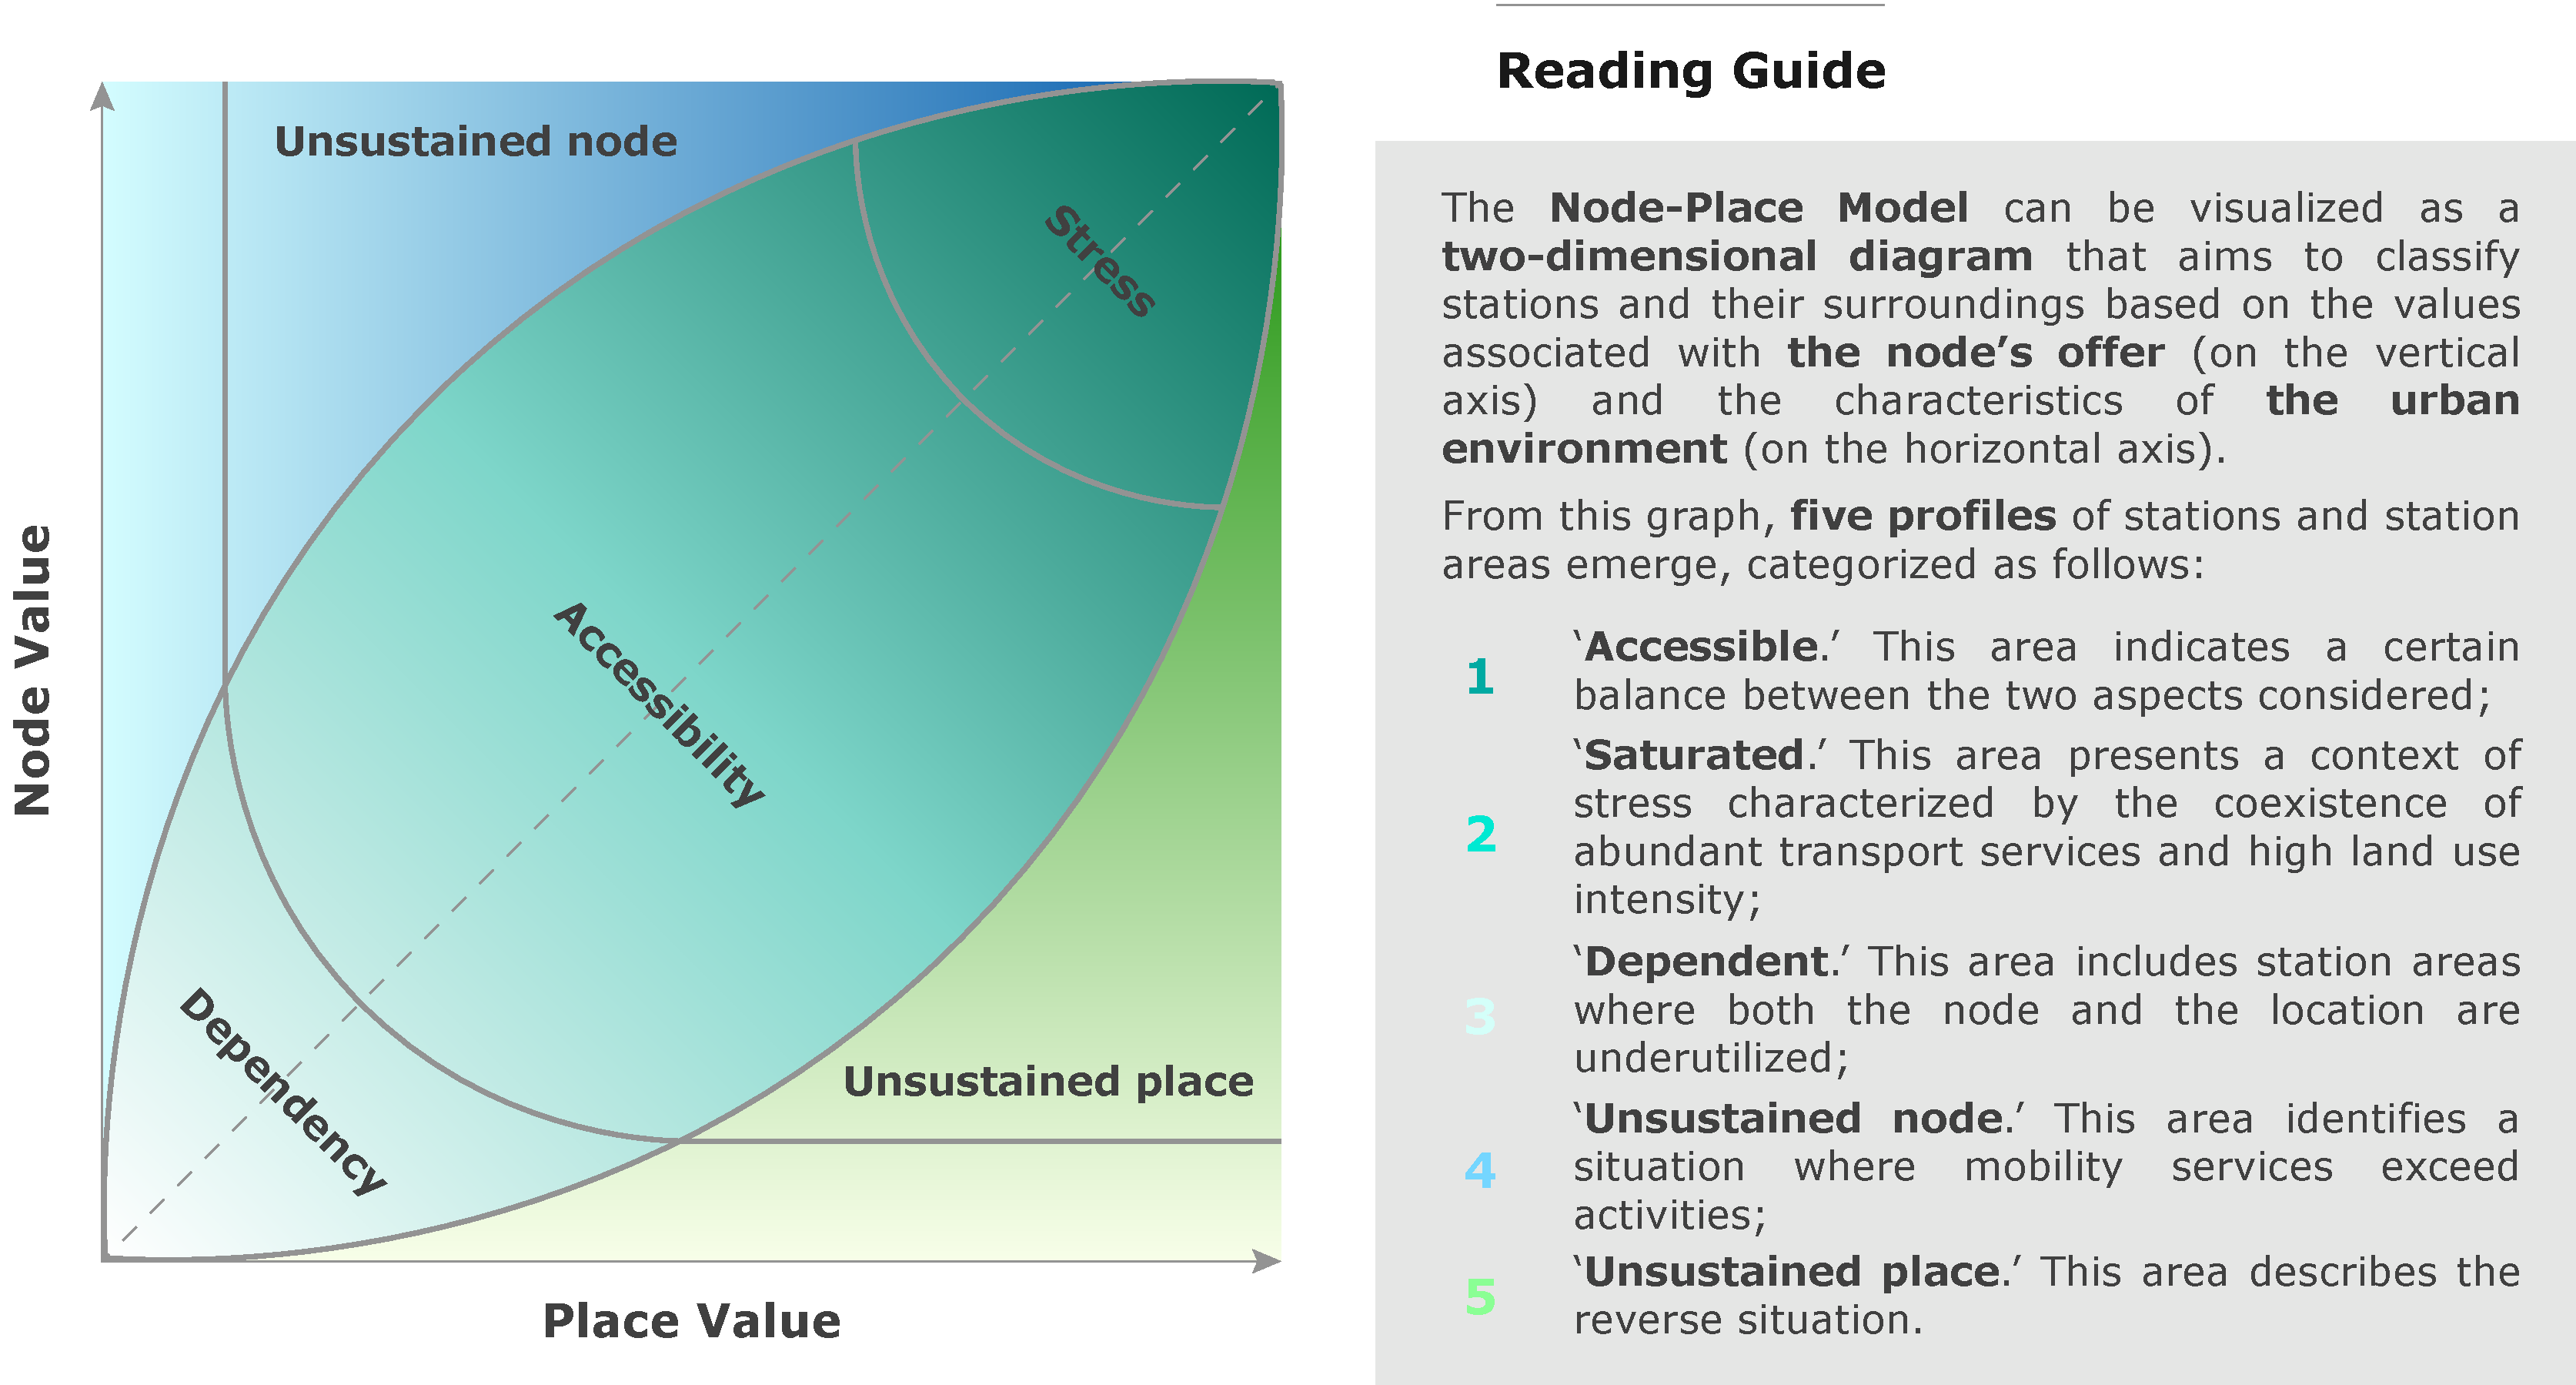
\includegraphics[width=1\columnwidth]{src/Figures/Chap-6/EN_NPART_Diagramme_Bertolini.pdf}}
        \vspace{5pt}
        \begin{flushright}\scriptsize{
        Source: Diagram created by \textcolor{blue}{Luca} \textcolor{blue}{\textcite[202]{bertolini_spatial_1999}}\index{Bertolini, Luca|pagebf} and reinterpreted by \textcolor{blue}{\textcite[243]{yang_tod_2021}}\index{Yang, Liu|pagebf}\index{Song, Xiaoyu|pagebf}
        \\
        Graphic adaptation: \textcolor{blue}{Dylan Moinse (2024)}
        }\end{flushright}
    \end{figure}

    % Diagram
The \acrshort{NPM} model proposes a diagrammatic and bidimensional approach to classify public transport nodes based on characteristics observed both at the physical stop level and the surrounding areas. In this diagram, initially developed by \textcolor{blue}{Luca} \textcolor{blue}{\textcite[344]{bertolini_nodes_1996}}\index{Bertolini, Luca|pagebf}, the intensity of land use around the station is represented on the x-axis, while the y-axis measures the accessibility of the node. This diagram allows for the distinction of five distinct typological configurations (see \hyperref[fig-chap6:schema-theorique-NP]{Figure~\ref{fig-chap6:schema-theorique-NP}}, page~\pageref{fig-chap6:schema-theorique-NP}):
\begin{customitemize}
    \item The \Commas{balance zone} is identified along the central diagonal of the diagram, signaling a relative equivalence between the values associated with the node and those linked to the place. The designation of this zone is also discussed in the scientific literature\footnote{~
        By classifying train stations in Brisbane (Australia), \textcolor{blue}{\textcite[55]{kamruzzaman_advance_2014}}\index{Kamruzzaman, Md.|pagebf}\index{Baker, Douglas|pagebf}\index{Washington, Simon|pagebf}\index{Turrell, Gavin|pagebf} confirmed that these nodes should be classified independently of the notion of balance. The authors illustrate this by presenting two stations identified with a \Commas{TOD potential,} one of which is balanced while the other is not. Furthermore, according to \textcolor{blue}{\textcite[194]{reusser_classifying_2008}}\index{Reusser, Dominik~E.|pagebf}\index{Loukopoulos, Peter|pagebf}\index{Stauffacher, Michael|pagebf}\index{Scholz, Roland~W.|pagebf}, if balance, as defined by \textcolor{blue}{\textcite[202]{bertolini_spatial_1999}}\index{Bertolini, Luca|pagebf}, is to be considered, it should be based on the size of the stations, thus providing a better context for each of them.
    }, \textcolor{blue}{\textcite[243]{yang_tod_2021}}\index{Yang, Liu|pagebf}\index{Song, Xiaoyu|pagebf} refers instead to the \Commas{accessible zone,} referring to the definition of accessibility combining mobility and the urban environment;
    \item The \Commas{stress zone} illustrates a context where the transport supply and the diversity of human activities are intense, generating maximum interactions;
    \item The \Commas{dependency zone} characterizes train station districts where the values of the node and the place are coherent but underutilized;
    \item The \Commas{unbalanced node zone} is identified when transport infrastructure and services exceed land use;
    \item The \Commas{unbalanced place zone} describes the opposite situation, where activities dominate over the available public transport supply.
\end{customitemize}%%Translated%%

    % Transition
A model such as the \acrshort{NPM} cannot accommodate a universal approach, typified by the expression \Commas{a generic model [for all territories]} (\textsl{one-size fits all}), especially when it comes to implementing the principles of \acrshort{TOD}. The need to adapt recommendations to effectively guide public policies requires a thorough analysis of the territorial context surrounding public transport stations. This approach is supported by the work of \textcolor{blue}{\textcite[678-679]{zemp_classifying_2011}}\index{Zemp, Stefan|pagebf}\index{Stauffacher, Michael|pagebf}\index{Lang, Daniel~J.|pagebf}\index{Scholz, Roland~W.|pagebf}, in their article titled \foreignlanguage{english}{\textsl{Classifying railway stations for strategic transport and land use planning: Context matters!}}, where the importance of the geographical context is explicitly emphasized in the process of classifying train stations. In contrast, excessive simplification, which neglects the specific context in which each station operates, may lead to erroneous assessments, as questioned by \textcolor{blue}{\textcite[2]{cao_coordination_2020}}\index{Cao, Zhejing|pagebf}\index{Asakura, Yasuo|pagebf}\index{Tan, Zongbo|pagebf}. The \acrshort{NPM} modeling highlights the local specificities of each site for a specific type of \acrshort{TOD}, rather than the binary question of its general suitability, according to \textcolor{blue}{\textcite[55]{kamruzzaman_advance_2014}}\index{Kamruzzaman, Md.|pagebf}\index{Baker, Douglas|pagebf}\index{Washington, Simon|pagebf}\index{Turrell, Gavin|pagebf}. The model's ability to adjust in order to more accurately reflect the complexity of the urban environments in which transport stations are embedded is therefore validated by the scientific literature, demonstrating its applicability across a variety of urban contexts.%%Translated%%

    % 6.1.2.
    \needspace{1\baselineskip} % Reserve space
\subsection{State of the Art of an Advanced and Gradually Enriched Model
    \label{chap6:litterature-etat-art}
    }

    % Growing Interest in the Model
Since 2007, the number of studies dedicated to this approach has continued to grow significantly. This trend is highlighted in the systematic literature review published by \textcolor{blue}{\textcite[383]{ibrahim_planning_2022}}\index{Ibrahim, Sara|pagebf}\index{Ayad, Hany|pagebf}\index{Saadallah, Dina|pagebf}. Over the past twenty years, the model has been implemented in a variety of geographical contexts, mainly in East and South Asia as well as Northern Europe \textcolor{blue}{\autocite[1]{caset_integrating_2020}}\index{Caset, Freke|pagebf}\index{Blainey, Simon|pagebf}\index{Derudder, Ben|pagebf}\index{Boussauw, Kobe|pagebf}\index{Witlox, Frank|pagebf}, and has been adapted to different application scales, ranging from rail corridors to regions, and even to the national level. The \acrshort{NPM} has been carried out by both scientific communities and various planning organizations, thus demonstrating its transcontinental flexibility \textcolor{blue}{\autocite[1]{caset_integrating_2020}}\index{Caset, Freke|pagebf}\index{Blainey, Simon|pagebf}\index{Derudder, Ben|pagebf}\index{Boussauw, Kobe|pagebf}\index{Witlox, Frank|pagebf}.%%Translated%%

    % Figure NPM Chronology
    \begin{figure}[h!]\vspace*{4pt}
        \caption{Chronological Evolution of Studies on the Node-Place Model.}
        \label{fig-chap6:litterature-chronologie}
        \centerline{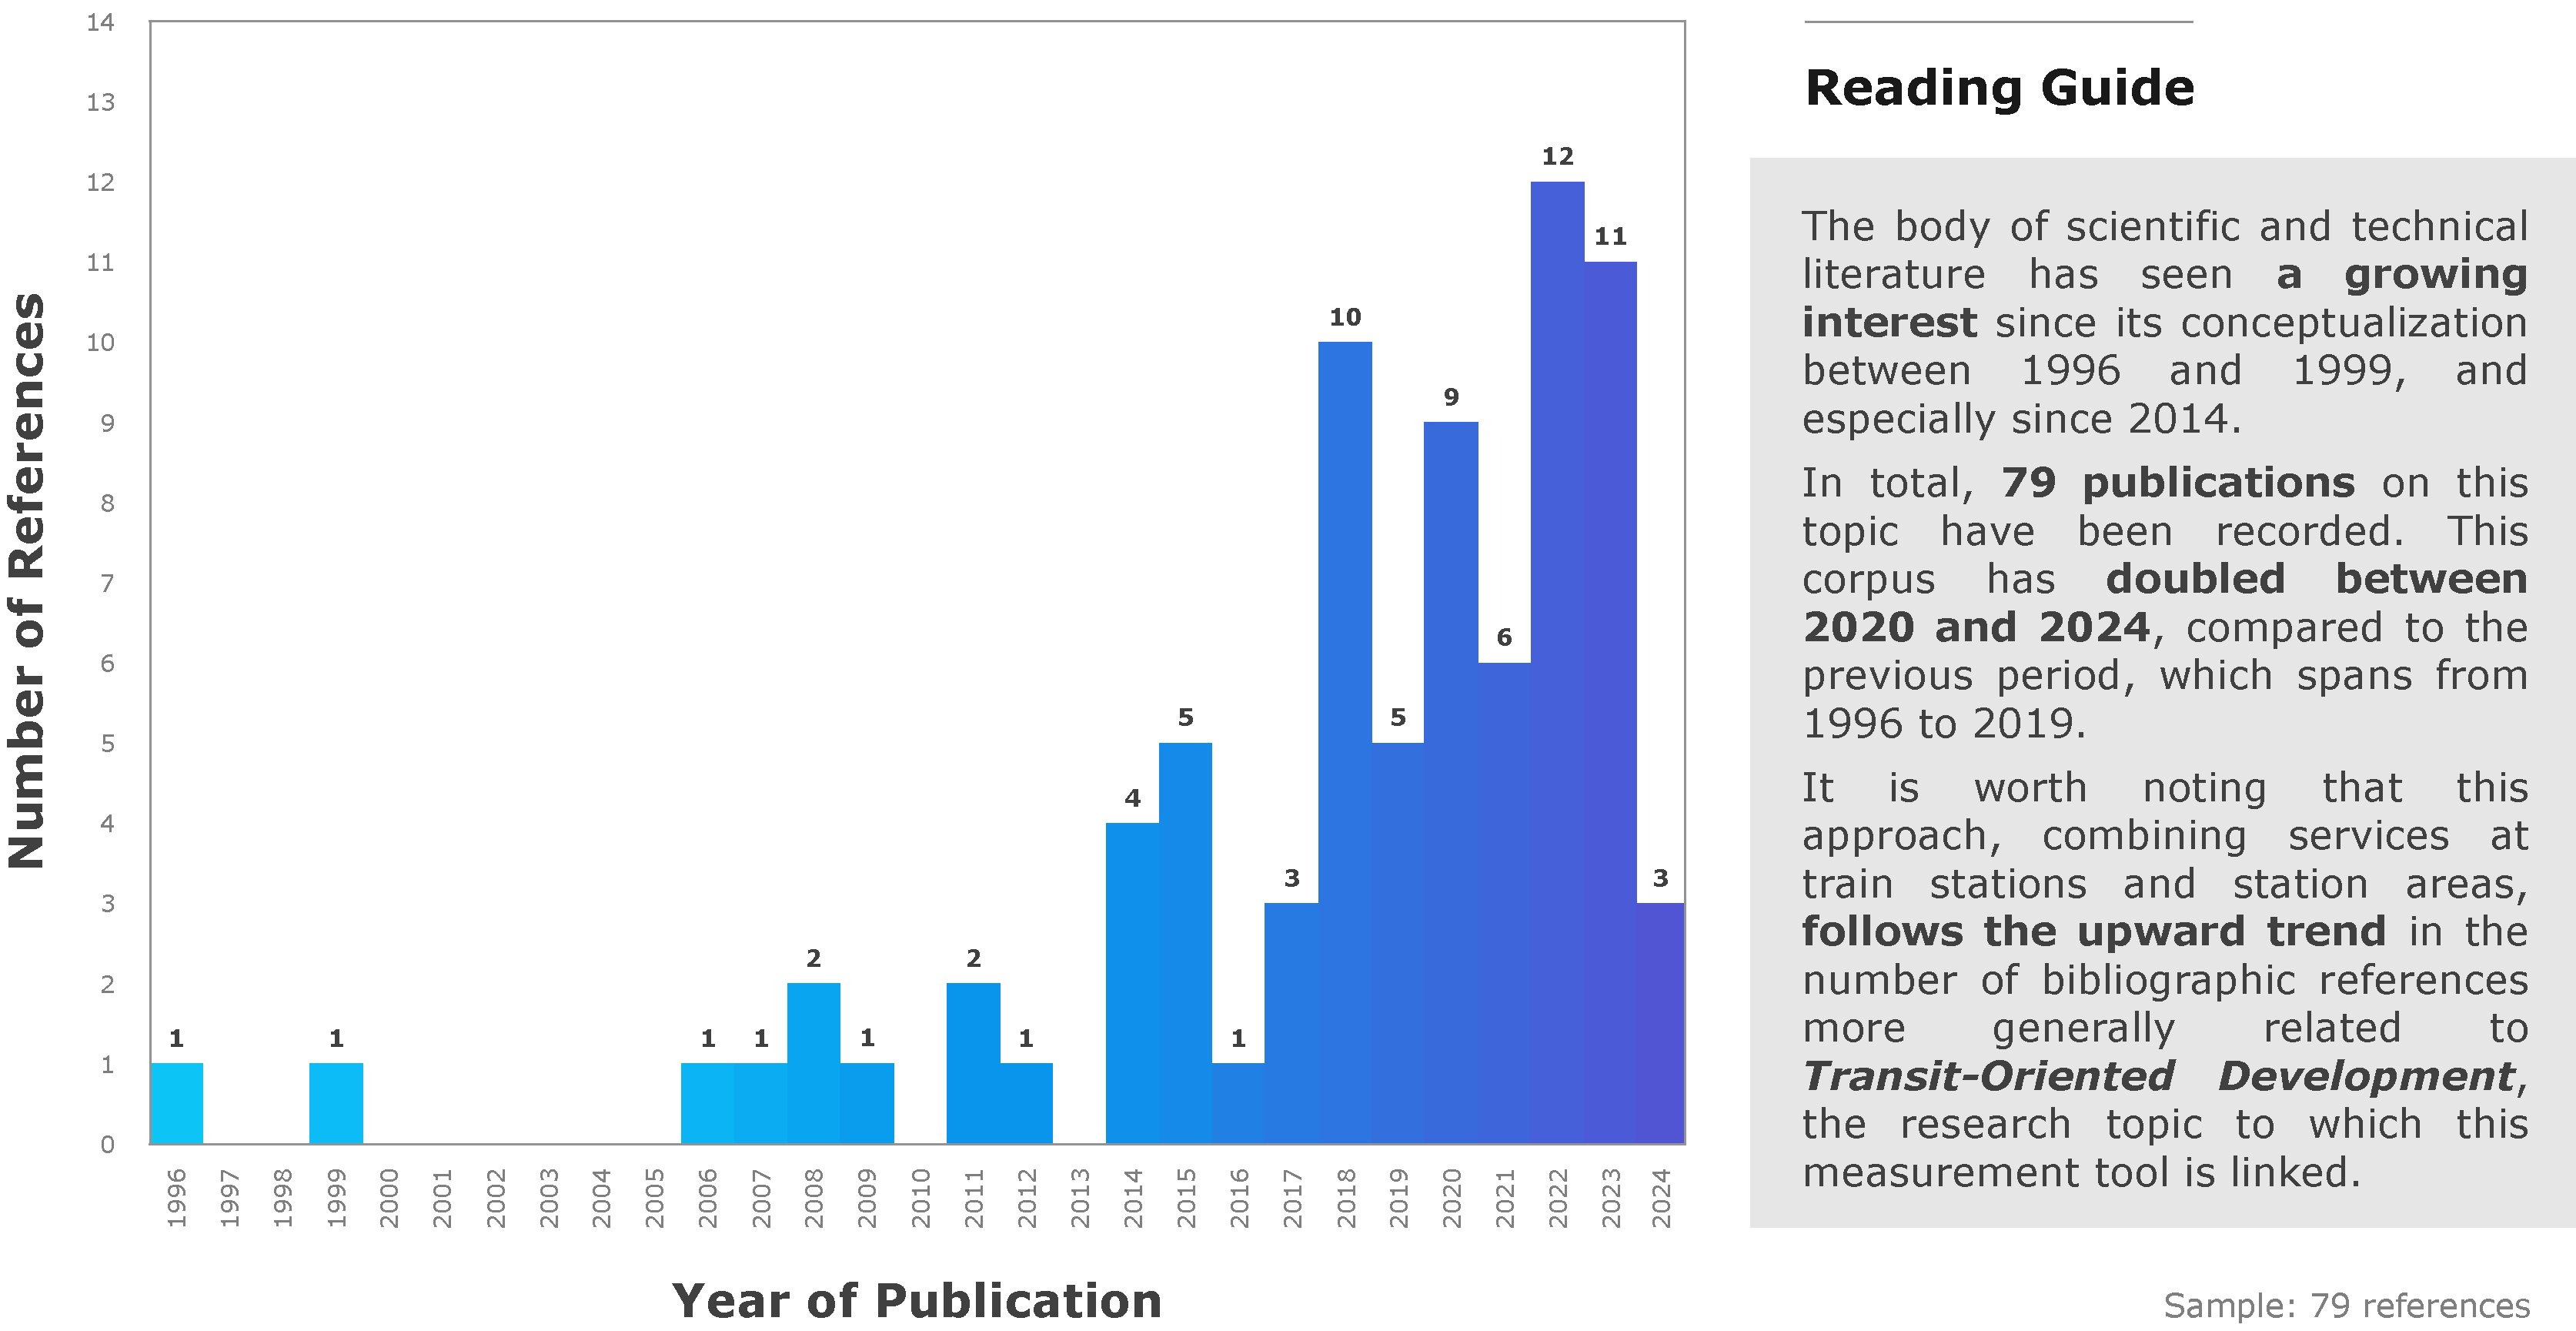
\includegraphics[width=1\columnwidth]{src/Figures/Chap-6/EN_NPART_Chronologie.pdf}}
        \vspace{5pt}
        \begin{flushright}\scriptsize{
        Realization: \textcolor{blue}{Dylan Moinse (2024)}
        \\
        Authors: \acrshort{NPART} Research Project
        }\end{flushright}
    \end{figure}

    % Chronological Results
As part of the literature review conducted on the \acrshort{NPM}, we identified a total of 79 bibliographic references that explicitly use this approach. These contributions were produced between 1996, the year marking the conceptualization of the model, and the beginning of 2024, when this bibliographic research was carried out. This corpus thus includes 69 articles, book chapters, and conference proceedings, as well as 5 technical reports, 3 Master's theses, and 2 doctoral dissertations. This initial chronological analysis confirms the growing interest in the \acrshort{NPM} starting from 2014, with a particularly marked dynamic between 2020 and 2024, a period during which the number of publications doubled compared to the interval spanning from 1996 to 2019 (see \hyperref[fig-chap6:litterature-chronologie]{Figure~\ref{fig-chap6:litterature-chronologie}}, page~\pageref{fig-chap6:litterature-chronologie}). Furthermore, this progression aligns with the general trend of increasing studies on \acrshort{TOD}.%%Translated%%

    % 6.1.2.1.
    \needspace{1\baselineskip} % Reserve space
\subsubsection*{An Underutilized Method in the French Context
    \label{chap6:litterature-geographie}
    }

    % Geographical Distribution
Studies show significant disparities in the application of the \acrshort{NPM} model depending on geographical contexts. Among the 63 study areas identified, the contributions are concentrated in China (11 references) and the Netherlands (8 references), similar to the \acrfull{SLR} dedicated to a \acrfull{B-TOD}. In contrast, the United States, with only 2 studies, are virtually absent from this landscape. Thus, Asia emerges as the leading continent in the development of this quantitative tool, as evidenced by \hyperref[fig-chap6:repartition-geographique]{Map~\ref{fig-chap6:repartition-geographique}} (page~\pageref{fig-chap6:repartition-geographique}). Furthermore, no scientific publication employing this model has been recorded in France, except for a study conducted by the Île-de-France Urban Planning Institute \textcolor{blue}{\autocite[2]{iau_articulation_2017}}\index{IAU@\textsl{IAU}|pagebf}.%%Translated%%

    % NP Index Map
    \begin{carte}[h!]\vspace*{4pt}
        \caption{Geographical Distribution of Studies Using the Node-Place Model.}
        \label{fig-chap6:repartition-geographique}
        \centerline{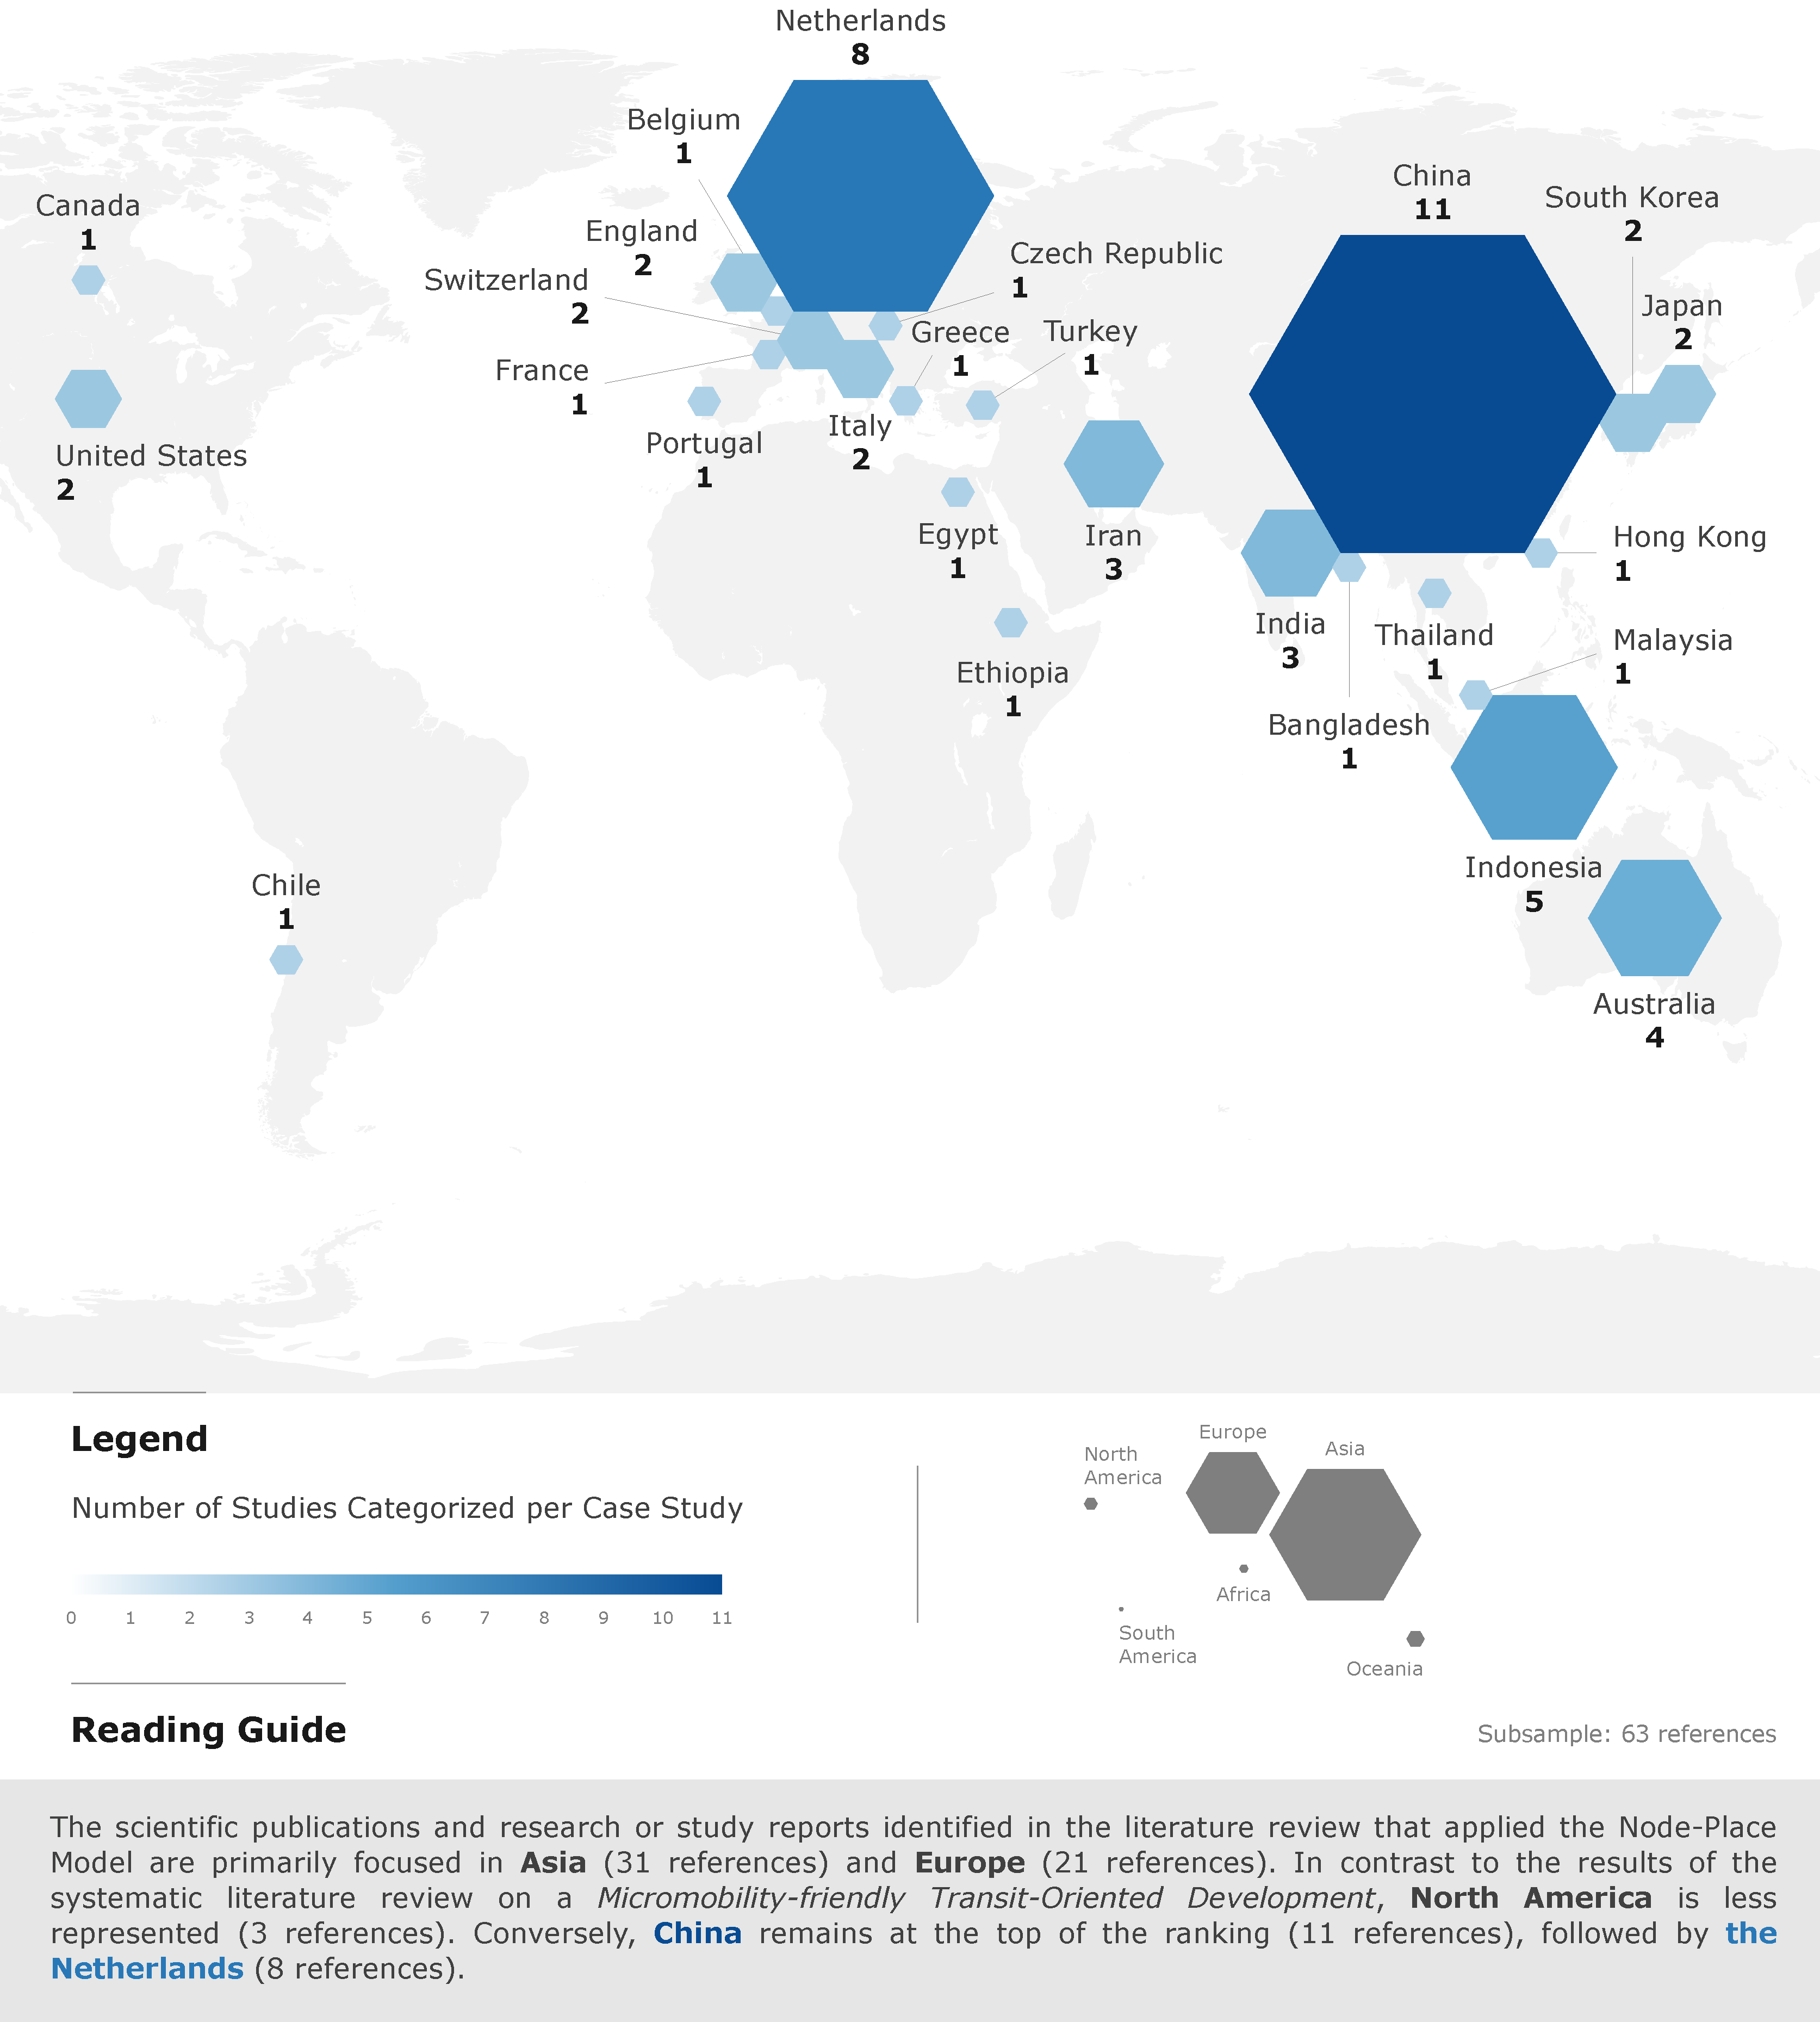
\includegraphics[width=1\columnwidth]{src/Figures/Chap-6/EN_NPART_Repartition_geographique.pdf}}
        \vspace{5pt}
        \begin{flushright}\scriptsize{
        Realization: \textcolor{blue}{Dylan Moinse (2024)}
        \\
        Authors: \acrshort{NPART} Research Project
        }\end{flushright}
    \end{carte}

    % Studies by Country: Asia
In Asia, we identified 31 academic contributions and research reports utilizing the \acrshort{NPM} model. China stands out with 11 studies, highlighting international metropolises such as Beijing \textcolor{blue}{\autocites[5]{liao_evaluating_2022}[43]{lyu_developing_2016}}\index{Liao, Cong|pagebf}\index{Scheuer, Bronte|pagebf}\index{Lyu, Guowei|pagebf}\index{Bertolini, Luca|pagebf}\index{Pfeffer, Karin|pagebf}, Chengdu \textcolor{blue}{\autocites[3]{amini_pishro_node_2022}[3]{amini_pishro_integrated_2023}[2]{ma_node-place_2022}}\index{Ma, Jiexi|pagebf}\index{Shen, Zhongwei|pagebf}\index{Xie, Yi|pagebf}\index{Liang, Pengpeng|pagebf}\index{Yu, Bingjie|pagebf}\index{Chen, Li|pagebf}\index{Amini Pishro, Ahad|pagebf}\index{Yang, Qihong|pagebf}\index{Zhang, Shiquan|pagebf}\index{Amini Pishro, Mojdeh|pagebf}\index{Zhang, Zhengrui|pagebf}\index{Zhao, Yana|pagebf}\index{Postel, Victor|pagebf}\index{Huang, Dengshi|pagebf}\index{Li, WeiYu|pagebf}\index{Amini Pishro, Ahad|pagebf}\index{L'Hostis, Alain|pagebf}\index{Chen, Dong|pagebf}\index{Chen, Mojdeh|pagebf}\index{Amini Pishro, Mojdeh|pagebf}\index{Zhang, Zhengrui|pagebf}\index{Li, Jun|pagebf}\index{Zhao, Yuandi|pagebf}\index{Zhang, Lili|pagebf}\index{Shen, Zhongwei|pagebf}\index{Xie, Yi|pagebf}\index{Liang, Pengpeng|pagebf}\index{Yu, Bingjie|pagebf}\index{Chen, Li|pagebf}, Ningbo \textcolor{blue}{\autocite[246]{yang_tod_2021}}\index{Yang, Liu|pagebf}\index{Song, Xiaoyu|pagebf} and Shanghai \textcolor{blue}{\autocites[446]{chen_node-place_2015}[4]{dou_integrating_2021}[273]{li_transit_2019}[8]{su_deciphering_2022}}\index{Su, Shiliang|pagebf}\index{Wang, Zhuolun|pagebf}\index{Li, Bozhao|pagebf}\index{Kang, Mengjun|pagebf}\index{Li, Zekun|pagebf}\index{Han, Zixuan|pagebf}\index{Xin, Jing|pagebf}\index{Luo, Xin|pagebf}\index{Su, Shiliang|pagebf}\index{Weng, Min|pagebf}\index{Chen, Xueming|pagebf}\index{Lin, Lin|pagebf}\index{Wang, Yandong|pagebf}\index{Dong, Shihai|pagebf}\index{Dou, Mingxuan|pagebf}. Two comparative approaches were also conducted, the first along the Yangtze Delta, including Shanghai, Nanjing, Wuhan, and Chongqing \textcolor{blue}{\autocite[629]{wei_classifying_2023}}\index{Wei, Sheng|pagebf}\index{Wang, Lei|pagebf} and the second between Beijing, Hangzhou, Shanghai, Shenzhen, and Wuhan \textcolor{blue}{\autocite[11]{su_transit-oriented_2021}}\index{Su, Shiliang|pagebf}\index{Zhang, Hui|pagebf}\index{Wang, Miao|pagebf}\index{Weng, Min|pagebf}\index{Kang, Mengjun|pagebf}. In Indonesia, the model has been applied in 5 studies, covering the metropolises of Jakarta \textcolor{blue}{\autocites[7]{arliani_measuring_2023}[47]{enjeri_characteristics_2020}[27]{taki_re-assessing_2017}}\index{Arliani, Vani|pagebf}\index{Sjafruddin, Ade|pagebf}\index{Santoso, Idwan|pagebf}\index{Winarso, Haryo|pagebf}\index{Taki, Herika|pagebf}\index{Maatouk, Mohamed|pagebf}\index{Qurnfulah, Emad|pagebf}\index{Enjeri, Tomi|pagebf}\index{Widyawati, Sumadio|pagebf}\index{Ash Shidiq, Iqbal|pagebf}, Depok \textcolor{blue}{\autocite[5]{sulistyaningrum_transit_2018}}\index{Sulistyaningrum, Subekti|pagebf}\index{Sumabrata, Jachrizal|pagebf} and Wates \textcolor{blue}{\autocite[15]{alfyan_node-place_2022}}\index{Alfyan, Muhammad Yusuf|pagebf}\index{Widyastuti, Dyah Titisari|pagebf}. In India, Delhi \textcolor{blue}{\autocite[6]{phani_kumar_identification_2020}}\index{Phani Kumar, Patnala|pagebf}\index{Ravi Sekhar, Chalumuri|pagebf}\index{Parida, Manoranjan|pagebf}, Ahmedabad \textcolor{blue}{\autocite[1018]{maheshwari_evaluating_2022}}\index{Maheshwari, Richa|pagebf}\index{Grigolon, Anna|pagebf}\index{Brussel, Mark|pagebf} and Noida \textcolor{blue}{\autocite[2]{kapoor_develop_2022}}\index{Kapoor, Sahil Singh|pagebf}\index{Brar, Tejwant Singh|pagebf} were the subjects of 3 studies, while in Iran, Tehran was represented through 3 scientific works \textcolor{blue}{\autocites[16]{monajem_evaluation_2015}[5]{motieyan_development_2018}[3]{pezeshknejad_evaluating_2020}}\index{Monajem, Saeed|pagebf}\index{Ekram Nosratian, Farzan|pagebf}\index{Motieyan, Hamid|pagebf}\index{Mesgari, Mohammad Saadi|pagebf}\index{Pezeshknejad, Parsa|pagebf}\index{Monajem, Saeed|pagebf}\index{Mozafari, Hamid|pagebf}. Other regions in Asia include Seoul, South Korea \textcolor{blue}{\autocites[129]{kim_geographic_2018}[2]{rodriguez_typology_2020}}\index{Rodríguez, Daniel~A.|pagebf}\index{Kang, Chang-Deok|pagebf}\index{Kim, Hyojin|pagebf}\index{Sultana, Selima|pagebf}\index{Weber, Joe|pagebf}, Tokyo, Japan \textcolor{blue}{\autocites[3]{cao_coordination_2020}[48]{chorus_application_2011}}\index{Chorus, Paul|pagebf}\index{Bertolini, Luca|pagebf}\index{Cao, Zhejing|pagebf}\index{Asakura, Yasuo|pagebf}\index{Tan, Zongbo|pagebf}, Bangkok, Thailand \textcolor{blue}{\autocite[120]{supaprasert_transit-oriented_2021}}\index{Supaprasert, Srisamrit|pagebf}\index{Lohatepanont, Manoj|pagebf}\index{Visamitanan, Krisana|pagebf}, Dhaka, Bangladesh \textcolor{blue}{\autocites[11]{uddin_framework_2023}[6]{uddin_revolutionizing_2023}}\index{Uddin, Md Anwar|pagebf}\index{Hoque, Md Shamsul|pagebf}\index{Tamanna, Tahsin|pagebf}\index{Adiba, Saima|pagebf}\index{Muniruzzaman, Shah Md|pagebf}\index{Parvez, Mohammad Shahriyar|pagebf}\index{Bin Kabir, Sadib|pagebf}, Kuala Lumpur, Malaysia \textcolor{blue}{\autocite[249]{khalid_evaluating_2023}}\index{Khalid, Nurul Shakila|pagebf}\index{Samsudin, Noor Aimran|pagebf} and Hong Kong \textcolor{blue}{\autocite[2]{zhou_introducing_2023}}\index{Zhou, Mingzhi|pagebf}\index{Zhou, Jiali|pagebf}\index{Zhou, Jiangping|pagebf}\index{Lei, Shuyu|pagebf}\index{Zhao, Zhan|pagebf}.%%Translated%%

    % Studies by Country: Europe
In Europe, 21 bibliographic references were analyzed, revealing a predominance of the Netherlands, with 8 studies, including doctoral theses and Master's dissertations, among which is a large-scale national study \textcolor{blue}{\autocite[273]{debrezion_modelling_2009}}\index{Debrezion, Ghebreegziabiher|pagebf}\index{Pels, Eric|pagebf}\index{Rietveld, Piet|pagebf}. These works primarily focus on studying the metropolitan region of Arnhem-Nijmegen \textcolor{blue}{\autocites[309]{huang_measuring_2018}[11]{lukman_development_2014}[132]{singh_measuring_2014}[24]{singh_measuring_2015}[101]{singh_measuring_2017}[268]{singh_planning_2018}}\index{Huang, Runjie|pagebf}\index{Grigolon, Anna|pagebf}\index{Madureira, Ana Mafalda|pagebf}\index{Brussel, Mark|pagebf}\index{Singh, Yamini Jain|pagebf}\index{Fard, Pedram|pagebf}\index{Zuidgeest, Mark|pagebf}\index{Brussel, Mark|pagebf}\index{Maarseveen, Martin van|pagebf}\index{Flacke, Johannes|pagebf}\index{Lukman, Azhari|pagebf}\index{Lukman, Azhari|pagebf}\index{Singh, Yamini Jain|pagebf} and the metropolitan region of the Randstad \textcolor{blue}{\autocites[203]{bertolini_spatial_1999}[771]{duffhues_breaking_2014}[8]{groenendijk_incorporating_2018}}\index{Bertolini, Luca|pagebf}\index{Groenendijk, Laura|pagebf}\index{Rezaei, Jafar|pagebf}\index{Almeida Correia, Gonçalo Homem de|pagebf}\index{Duffhues, Jan|pagebf}\index{Mayer, Igor~S.|pagebf}\index{Nefs, Merten|pagebf}\index{Vliet, Mirte van der|pagebf}. In addition to the Netherlands, other European countries have also applied this model exploring the relationship between networks and urbanism. In Turkey, studies focused on Ankara \textcolor{blue}{\autocite[5]{ozgur-cevher_evaluating_2020}}\index{Ozgür-Cevher, Ozge|pagebf}\index{Altintasi, Oruc|pagebf}\index{Tuydes-Yaman, Hediye|pagebf}, while in Belgium, studies covered the regions of Brussels and Flanders \textcolor{blue}{\autocites[34]{caset_planning_2019}[2]{caset_integrating_2020}[500]{caset_measuring_2018}}\index{Caset, Freke|pagebf}\index{Blainey, Simon|pagebf}\index{Derudder, Ben|pagebf}\index{Boussauw, Kobe|pagebf}\index{Witlox, Frank|pagebf}\index{Vale, David~S.|pagebf}\index{Viana, Cláudia~M.|pagebf}. The Île-de-France region in France \textcolor{blue}{\autocite[2]{iau_articulation_2017}}\index{IAU@\textsl{IAU}|pagebf}, Lisbon, Portugal \textcolor{blue}{\autocites[73]{vale_transit-oriented_2015}[286]{vale_extended_2018}}\index{Vale, David~S.|pagebf}\index{Viana, Cláudia~M.|pagebf}\index{Pereira, Mauro|pagebf}, London \textcolor{blue}{\autocite[4]{zhang_network_2019}}\index{Zhang, Yuerong|pagebf}\index{Marshall, Stephen|pagebf}\index{Manley, Ed.~J.|pagebf} and Manchester \textcolor{blue}{\autocite[4]{zheng_classifying_2023}}\index{Zheng, Lingwei|pagebf}\index{Austwick, Martin Zaltz|pagebf}, England, Naples \textcolor{blue}{\autocite[291]{papa_tod_2018}}\index{Papa, Enrica|pagebf}\index{Carpentieri, Gerardo|pagebf}\index{Angiello, Gennaro|pagebf} and the Campania region \textcolor{blue}{\autocite[114]{nigro_land_2019}}\index{Nigro, Antonio|pagebf}\index{Bertolini, Luca|pagebf}\index{Moccia, Francesco Domenico|pagebf}, Italy, Ostrava, Czech Republic \textcolor{blue}{\autocite[142]{ivan_evaluation_2012}}\index{Ivan, Igor|pagebf}\index{Boruta, Tomáš|pagebf}\index{Horak, Jiri|pagebf} and Thessaloniki, Greece \textcolor{blue}{\autocite[8]{papagiannakis_transit-oriented_2021}}\index{Papagiannakis, Apostolos|pagebf}\index{Vitopoulou, Athina|pagebf}\index{Yiannakou, Athena|pagebf} have also been the subjects of empirical investigations. In Switzerland, 2 studies using a national scale were conducted \textcolor{blue}{\autocites[194]{reusser_classifying_2008}[672]{zemp_classifying_2011}}\index{Reusser, Dominik~E.|pagebf}\index{Loukopoulos, Peter|pagebf}\index{Stauffacher, Michael|pagebf}\index{Scholz, Roland~W.|pagebf}\index{Zemp, Stefan|pagebf}\index{Stauffacher, Michael|pagebf}\index{Lang, Daniel~J.|pagebf}\index{Scholz, Roland~W.|pagebf}, while a study by \textcolor{blue}{\textcite[74]{papa_accessibility_2015}}\index{Papa, Enrica|pagebf}\index{Bertolini, Luca|pagebf} compares the cities of Amsterdam, Helsinki, Munich, Naples, Rome, and Zurich.%%Translated%%

    % Studies by Country: Other Continents
Outside of the Asian and European continents, research using the \acrshort{NPM} model is rarer. In Australia, the cities of Brisbane \textcolor{blue}{\autocites[57]{kamruzzaman_advance_2014}[4]{lee_passive_2024}}\index{Lee, Jinwoo Brian|pagebf}\index{Salih, Samal Hama|pagebf}\index{Kamruzzaman, Md.|pagebf}\index{Baker, Douglas|pagebf}\index{Washington, Simon|pagebf}\index{Turrell, Gavin|pagebf}, Perth \textcolor{blue}{\autocite[2]{olaru_place_2019}}\index{Olaru, Doina|pagebf}\index{Moncrieff, Simon|pagebf}\index{McCarney, Gary|pagebf}\index{Sun, Yuchao|pagebf}\index{Reed, Tristan|pagebf}\index{Pattison, Cate|pagebf}\index{Smith, Brett|pagebf}\index{Biermann, Sharon|pagebf} and Sydney \textcolor{blue}{\autocites[3]{cummings_does_2022}[5]{zhang_make_2023}}\index{Cummings, Christopher|pagebf}\index{Mahmassani, Hani|pagebf}\index{Zhang, Mengyuan|pagebf}\index{Lee, Jinwoo Brian|pagebf} have been explored. In the United States, New York City \textcolor{blue}{\autocite[6]{baghestani_application_2023}}\index{Cummings, Christopher|pagebf}\index{Mahmassani, Hani|pagebf}\index{Baghestani, Amirhossein|pagebf}\index{Najafabadi, Shirin|pagebf}\index{Salem, Azarakhsh|pagebf}\index{Jiang, Ziqi|pagebf}\index{Tayarani, Mohammad|pagebf}\index{Gao, Oliver|pagebf} and in Canada, Montreal \textcolor{blue}{\autocite[80]{robillard_transit-oriented_2024}}\index{Robillard, Arianne|pagebf}\index{Boisjoly, Geneviève|pagebf}\index{Lierop, Dea van|pagebf} have been studied. In Egypt, Alexandria \textcolor{blue}{\autocite[242]{ibrahim_measuring_2023}}\index{Ibrahim, Sara|pagebf}\index{Ayad, Hany|pagebf}\index{Turki, Eslam|pagebf}\index{Saadallah, Dina|pagebf}, in Ethiopia, Addis Ababa \textcolor{blue}{\autocite[608]{teklemariam_determining_2020}}\index{Teklemariam, Eden Atsbeha|pagebf}\index{Shen, Zhongwei|pagebf} and in Chile, Santiago \textcolor{blue}{\autocite[87]{vecchio_estaciones_2021}}\index{Vecchio, Giovanni|pagebf} have been addressed by the model.%%Translated%%

    % Explanations of Geographical Distribution
These disparities in the geographical distribution of studies can be interpreted by the definition of \acrshort{TOD} strategies tailored to the specific contexts of mobility systems and existing urban configurations. According to \textcolor{blue}{\textcite[]{bertolini_cities_2015}}\index{Bertolini, Luca|pagebf}\index{Spit, Tejo|pagebf} as well as \textcolor{blue}{\textcite[]{ivan_evaluation_2012}}\index{Ivan, Igor|pagebf}\index{Boruta, Tomáš|pagebf}\index{Horak, Jiri|pagebf}, in Europe, the approach mainly focuses on the redevelopment of existing train station neighborhoods, using the model to evaluate, on a larger scale, the opportunities for revitalizing stations and their immediate surroundings. \textcolor{blue}{\textcite[42]{lyu_developing_2016}}\index{Lyu, Guowei|pagebf}\index{Bertolini, Luca|pagebf}\index{Pfeffer, Karin|pagebf} emphasize that in North America and Australia, the focus is primarily on the recentralization of suburban areas around public transport stops, while in South America, \acrshort{TOD} is often seen as a way to reconnect and recentralize already dense urban development around nodes. In contrast, in Asia, \textcolor{blue}{\textcite[42]{lyu_developing_2016}}\index{Lyu, Guowei|pagebf}\index{Bertolini, Luca|pagebf}\index{Pfeffer, Karin|pagebf} consider that the main objective of the planning concept is to channel the growth of megacities along mass transit corridors in order to control urban sprawl.%%Translated%%

    % 6.1.2.2.
    \needspace{1\baselineskip} % Reserve space
\subsubsection*{An Evaluation at a Limited Geographical Scale
    \label{chap6:litterature-taille-urbaine}
    }

    % Urban Sizes
As shown by the various listings of studies distributed by continents and countries, very few studies focus on the implementation of the \acrshort{NPM} model in areas that are not part of a regional or international metropolis. This observation supports that of \textcolor{blue}{\textcite[111]{nigro_land_2019}}\index{Nigro, Antonio|pagebf}\index{Bertolini, Luca|pagebf}\index{Moccia, Francesco Domenico|pagebf}, who emphasizes the scarcity of research on the coordination between public transport and land use in areas that are sparsely or moderately dense, in economic decline, or incorporating \acrfull{HST} networks, due to the very large coverage that imposes constraints.%%Translated%%

    % Figure Sizes of Public Transport Networks
    \begin{figure}[h!]\vspace*{4pt}
        \caption{Size of public transport networks, in number of stations, integrated into the node-place model.}
        \label{fig-chap6:taille-reseaux-TC}
        \centerline{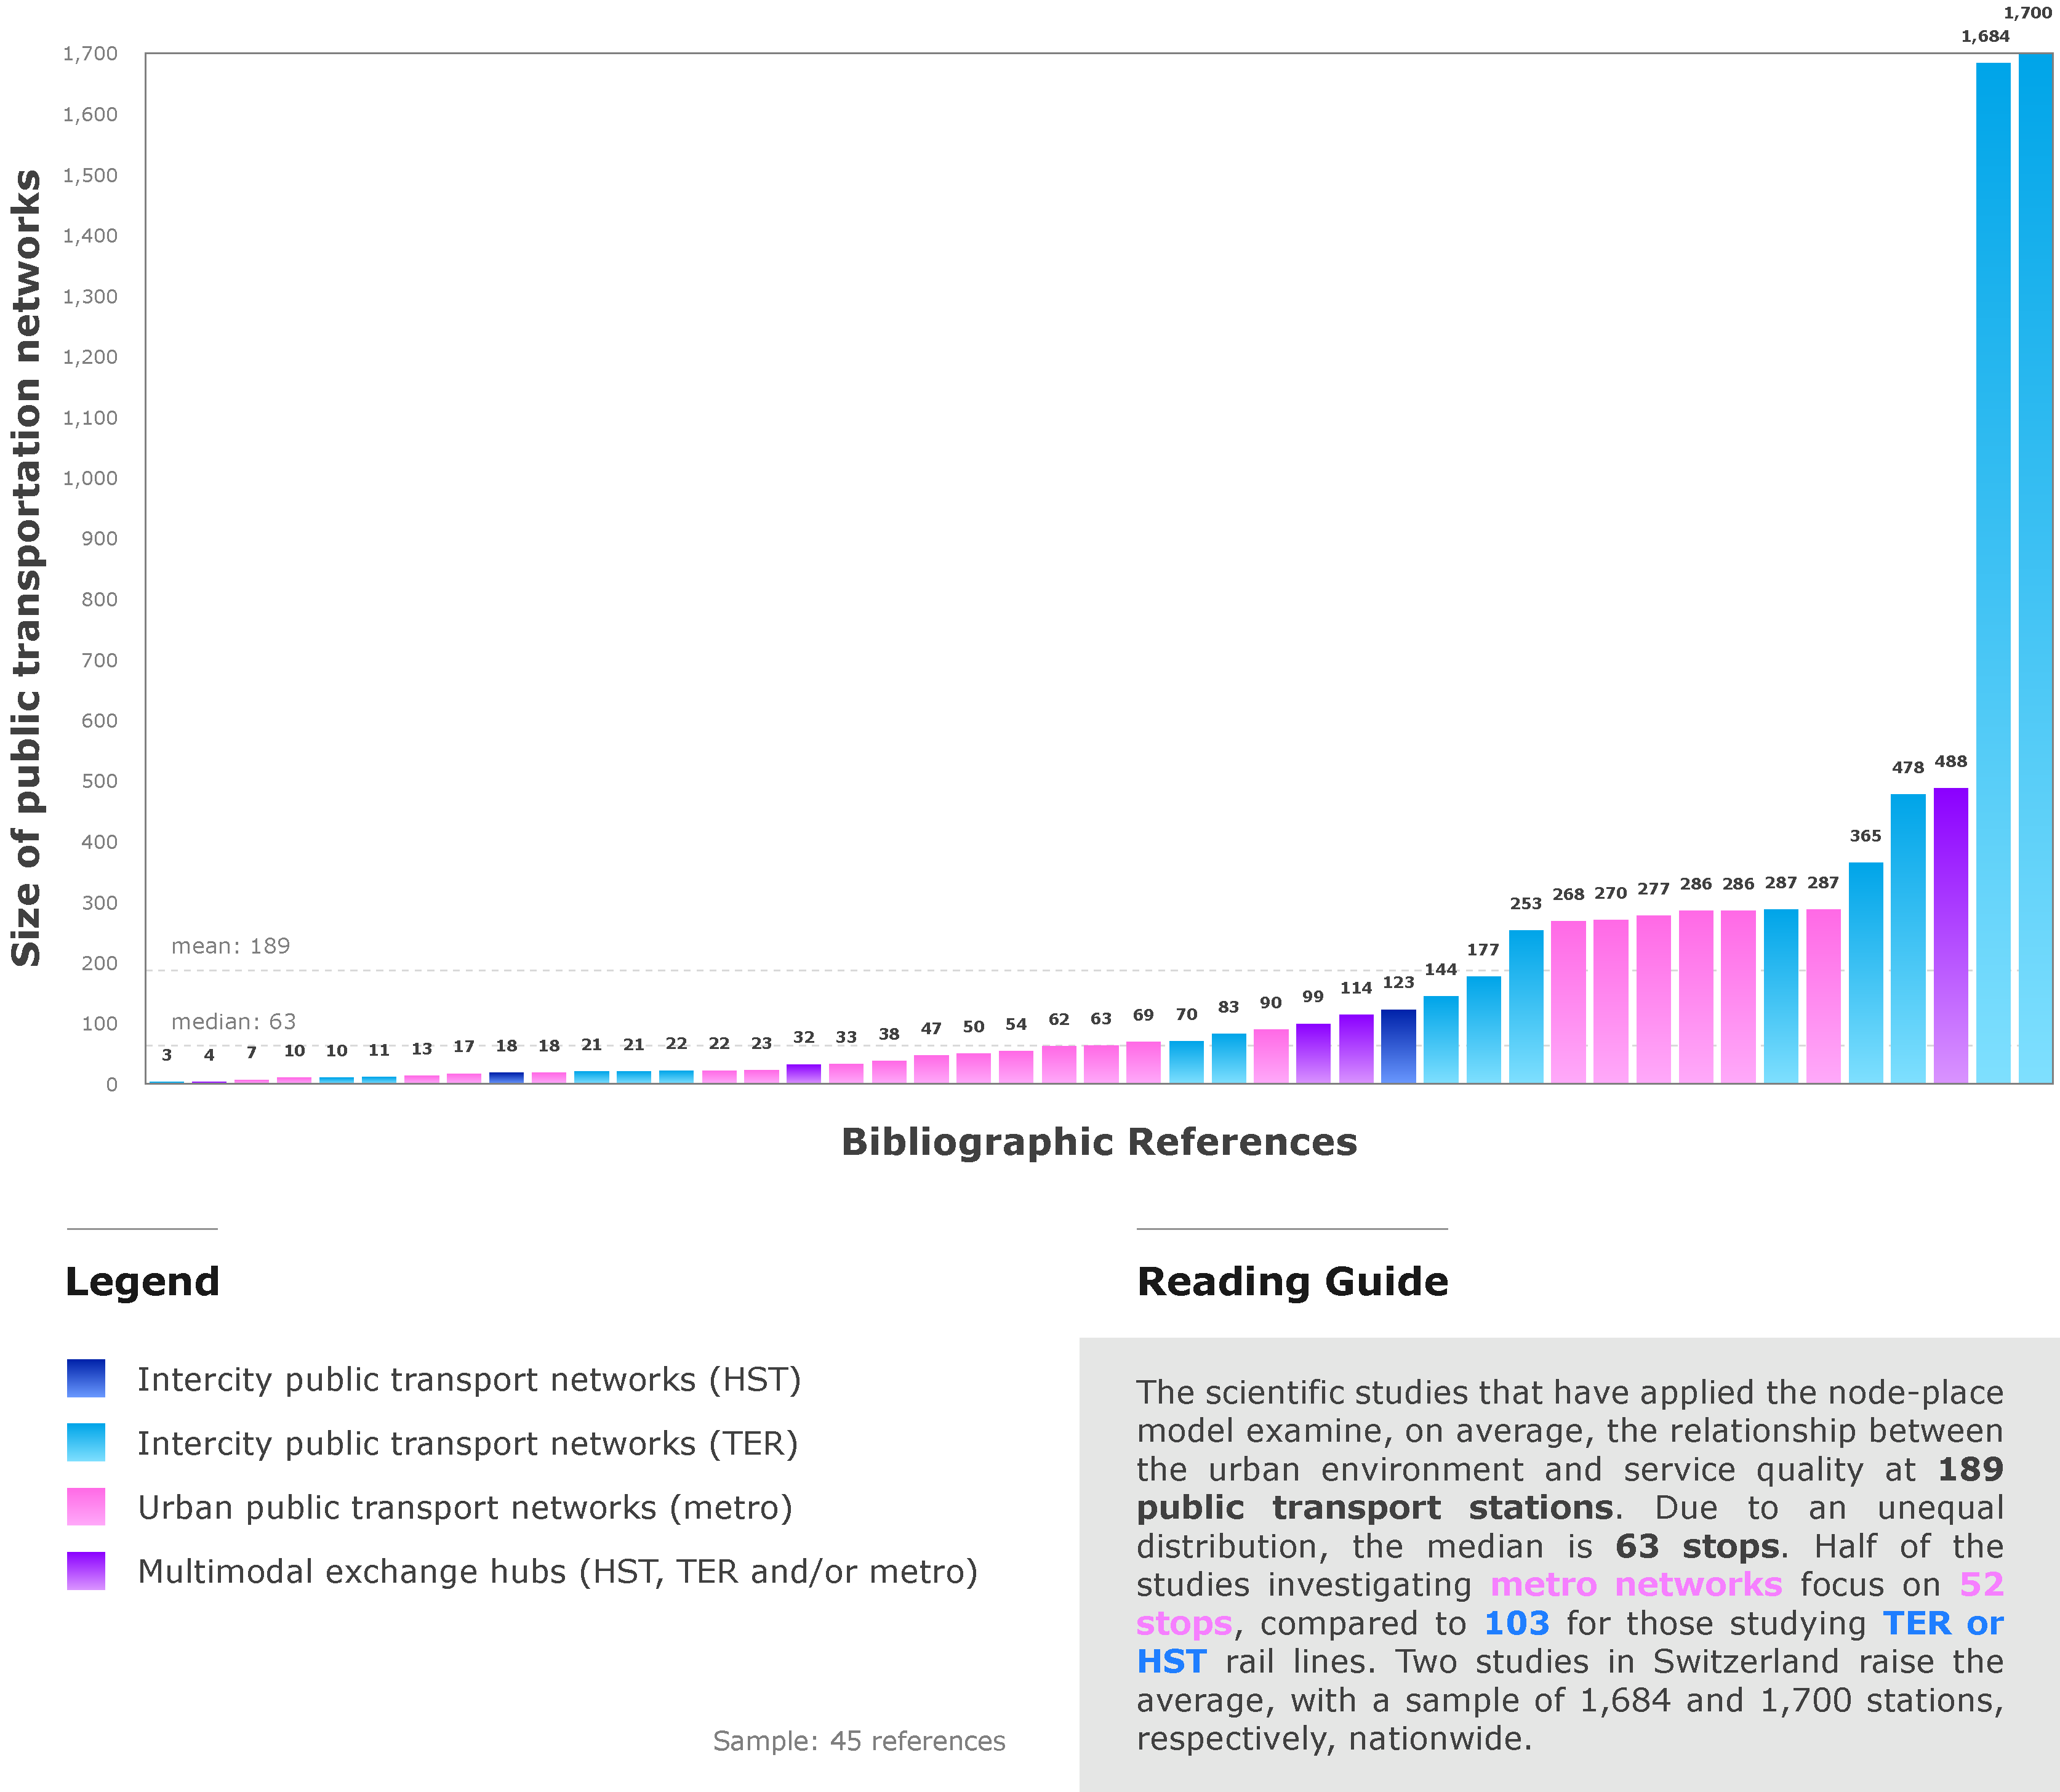
\includegraphics[width=1\columnwidth]{src/Figures/Chap-6/EN_NPART_Taille_reseaux_TC.pdf}}
        \vspace{5pt}
        \begin{flushright}\scriptsize{
        Realization: \textcolor{blue}{Dylan Moinse (2024)}
        \\
        Authors: \acrshort{NPART} Research Project
        }\end{flushright}
    \end{figure}

    % Sizes of Public Transport Networks
Another demonstration of the flexibility of the model in question is evident in the diversity of the size of the public transport networks examined, with values ranging from 3 to 1,700 stations within a defined operational perimeter. As illustrated by \hyperref[fig-chap6:taille-reseaux-TC]{Figure~\ref{fig-chap6:taille-reseaux-TC}} (page~\pageref{fig-chap6:taille-reseaux-TC}), this quantitative approach generally covers \acrfull{TER} or metro systems, with an average of 189 and a median of 63 nodes. In fact, half of the studies using the \acrshort{NPM} to examine metro systems focus on fewer than 52 stops, while those dedicated to \acrshort{TER} or \acrshort{HST} networks cover 103. Notably, two Swiss studies at the national scale have successfully adapted the model to a network comprising approximately 1,700 stations \textcolor{blue}{\autocites[194]{reusser_classifying_2008}[672]{zemp_classifying_2011}}\index{Zemp, Stefan|pagebf}\index{Stauffacher, Michael|pagebf}\index{Lang, Daniel~J.|pagebf}\index{Scholz, Roland~W.|pagebf}\index{Reusser, Dominik~E.|pagebf}\index{Loukopoulos, Peter|pagebf}\index{Stauffacher, Michael|pagebf}\index{Scholz, Roland~W.|pagebf}.%%Translated%%

    % Transition
The adaptability of the model to various geographical contexts and different forms of public transport systems illustrates its flexibility and its ability to evolve based on theoretical and empirical discussions since its initial development. This continuous enrichment is also evident in the diversity of synthetic indicators used to define it, as presented in the following section.%%Translated%%

    % 6.1.2.3.
    \needspace{1\baselineskip} % Reserve space
\subsubsection*{A Model That Gains Precision Through Adjustments
    \label{chap6:litterature-indicateurs}
    }

    % Introduction
Currently, there is no consensus on the selection of indicators to evaluate the functionality of nodes and places at public transport stations \textcolor{blue}{\autocites[446]{chen_node-place_2015}[194]{reusser_classifying_2008}}\index{Chen, Xueming|pagebf}\index{Lin, Lin|pagebf}\index{Wang, Yandong|pagebf}\index{Dong, Shihai|pagebf}\index{Reusser, Dominik~E.|pagebf}\index{Loukopoulos, Peter|pagebf}\index{Stauffacher, Michael|pagebf}\index{Scholz, Roland~W.|pagebf}. Various adaptations of the original \acrshort{NPM} model have been introduced \textcolor{blue}{\autocites[2]{lee_passive_2024}[20]{lukman_development_2014}}\index{Lukman, Azhari|pagebf}\index{Singh, Yamini Jain|pagebf}\index{Lee, Jinwoo Brian|pagebf}\index{Salih, Samal Hama|pagebf}. According to these authors, the ideal indicators for this model must meet five principles:
\begin{customitemize}
    \item The relevance and significance of the variable for \acrshort{TOD}, reflecting the variations between public transport stations;
    \item The practicability of the variable, which must be measurable and applicable;
    \item The clarity of the interpretation of the variable;
    \item The efficiency of the variable in terms of data availability and measurement methods;
    \item The reproducibility of the variable, which must be generic and applicable to contexts beyond the study area.
\end{customitemize}%%Translated%%

    % Initial Indicators
At the beginning of the development of the analytical model, \textcolor{blue}{Luca} \textcolor{blue}{\textcite[202-203]{bertolini_spatial_1999}}\index{Bertolini, Luca|pagebf} proposed the integration of a set of synthetic indicators, classified according to the dimensions of \Commas{node} and \Commas{place}. The first dimension includes criteria such as the number of directions accessible from a station, the daily service frequency, the number of stations accessible within a 45-minute journey, as well as the number of directions and the daily frequency of urban public transport networks. Additional factors include the distance to the nearest highway access\footnote{~
    A parallel can be drawn with the transport models mentioned earlier, from which the \acrshort{NPM} seeks to differentiate itself. While the classical model mainly focuses on the modal choice between private car and public transport, the \acrshort{NPM} captures part of this issue by integrating measures of road accessibility to compare it to that offered by public transport.
}, the capacity of car parking spaces, the length of cycling infrastructure, and the capacity of bicycle parking. The second dimension incorporates parameters such as the number of residents in the train station area, the number of employees distributed across four sectors of activity, and the degree of functional mix. For its part, the \textsl{Transportation Research Board} emphasized the need to focus on the most quantifiable aspects of \acrshort{TOD} to aggregate them into indices. The research organization \textcolor{blue}{\textcite{transportation_research_board_of_the_national_academies_transit_2007}}\index{Transportation Research Board@\textsl{Transportation Research Board}|pagebf} identified the most relevant indicators to calibrate the \acrshort{NPM} model, namely public transport ridership, density, the quality of public space design, the amount of mixed-use structures, pedestrian activity, property value increases, public perception, intermodal connections, and parking facility configurations.%%Translated%%

    % New Dimensions: Oriented
However, the model was quickly enriched with new indicators to address certain limitations identified in the scientific literature. First, \textcolor{blue}{\textcite[4-5]{zhang_make_2023}}\index{Zhang, Mengyuan|pagebf}\index{Lee, Jinwoo Brian|pagebf} estimated that the current model fails to optimally identify the functional connections between the urban environment and the node. They highlight a persistent confusion in distinguishing between a \acrshort{TOD} environment and a \acrfull{TAD} environment\footnote{~
    Taking the San Francisco Bay area as a case study, \textcolor{blue}{John Luciano} \textcolor{blue}{\textcite[3]{renne_transit-adjacent_2009}}\index{Renne, John Luciano|pagebf} conceptualizes \textsl{Transit-Adjacent Development}, describing real estate or urban development projects located near public transport stations but not designed to maximize their ridership. These projects, although adjacent to the stations, encourage car use through low density, a spatial predominance of parking lots, limited access to \gls{active modes}, and a lack of functional diversity. Unlike \acrshort{TOD}, \acrshort{TAD} is neither morphologically nor functionally integrated with public transport infrastructure.
}. To address this confusion, \textcolor{blue}{\textcite[271]{li_transit_2019}}\index{Li, Zekun|pagebf}\index{Han, Zixuan|pagebf}\index{Xin, Jing|pagebf}\index{Luo, Xin|pagebf}\index{Su, Shiliang|pagebf}\index{Weng, Min|pagebf} propose integrating a new dimension related to the connectivity of places and extending the \acrshort{NPM} model by adding a third dimension focused on the concept of \Commas{orientation,} borrowed from \acrshort{TOD} terminology.%%Translated%%

    % New Dimensions: Ridership
At the same time, research has directed the model towards integrating ridership at public transport stations, a paradoxically neglected aspect despite being one of the pillars of public transport-oriented urban development. \textcolor{blue}{\textcite[2]{cao_coordination_2020}}\index{Cao, Zhejing|pagebf}\index{Asakura, Yasuo|pagebf}\index{Tan, Zongbo|pagebf} and \textcolor{blue}{\textcite[3]{amini_pishro_node_2022}}\index{Amini Pishro, Ahad|pagebf}\index{L'Hostis, Alain|pagebf}\index{Chen, Dong|pagebf}\index{Chen, Mojdeh|pagebf}\index{Amini Pishro, Mojdeh|pagebf}\index{Zhang, Zhengrui|pagebf}\index{Li, Jun|pagebf}\index{Zhao, Yuandi|pagebf}\index{Zhang, Lili|pagebf} emphasize that previous studies have rarely considered ridership as an essential dimension of the \acrshort{NPM}. However, it reflects how travelers use public transport infrastructure and how ridership is influenced by the quality of the urban environment. The goal of such an extension of the model is therefore to systematically incorporate mobility demand into the model, as recommended by \textcolor{blue}{\textcite[2]{liao_evaluating_2022}}\index{Liao, Cong|pagebf}\index{Scheuer, Bronte|pagebf}.%%Translated%%

    % Figure Interconnections Literature Indicators
    \begin{figure}[h!]\vspace*{4pt}
        \caption{Network Analysis of the Selected Indicators in Developed Node-Place Models.}
        \label{fig-chap6:litterature-indicateurs}
        \centerline{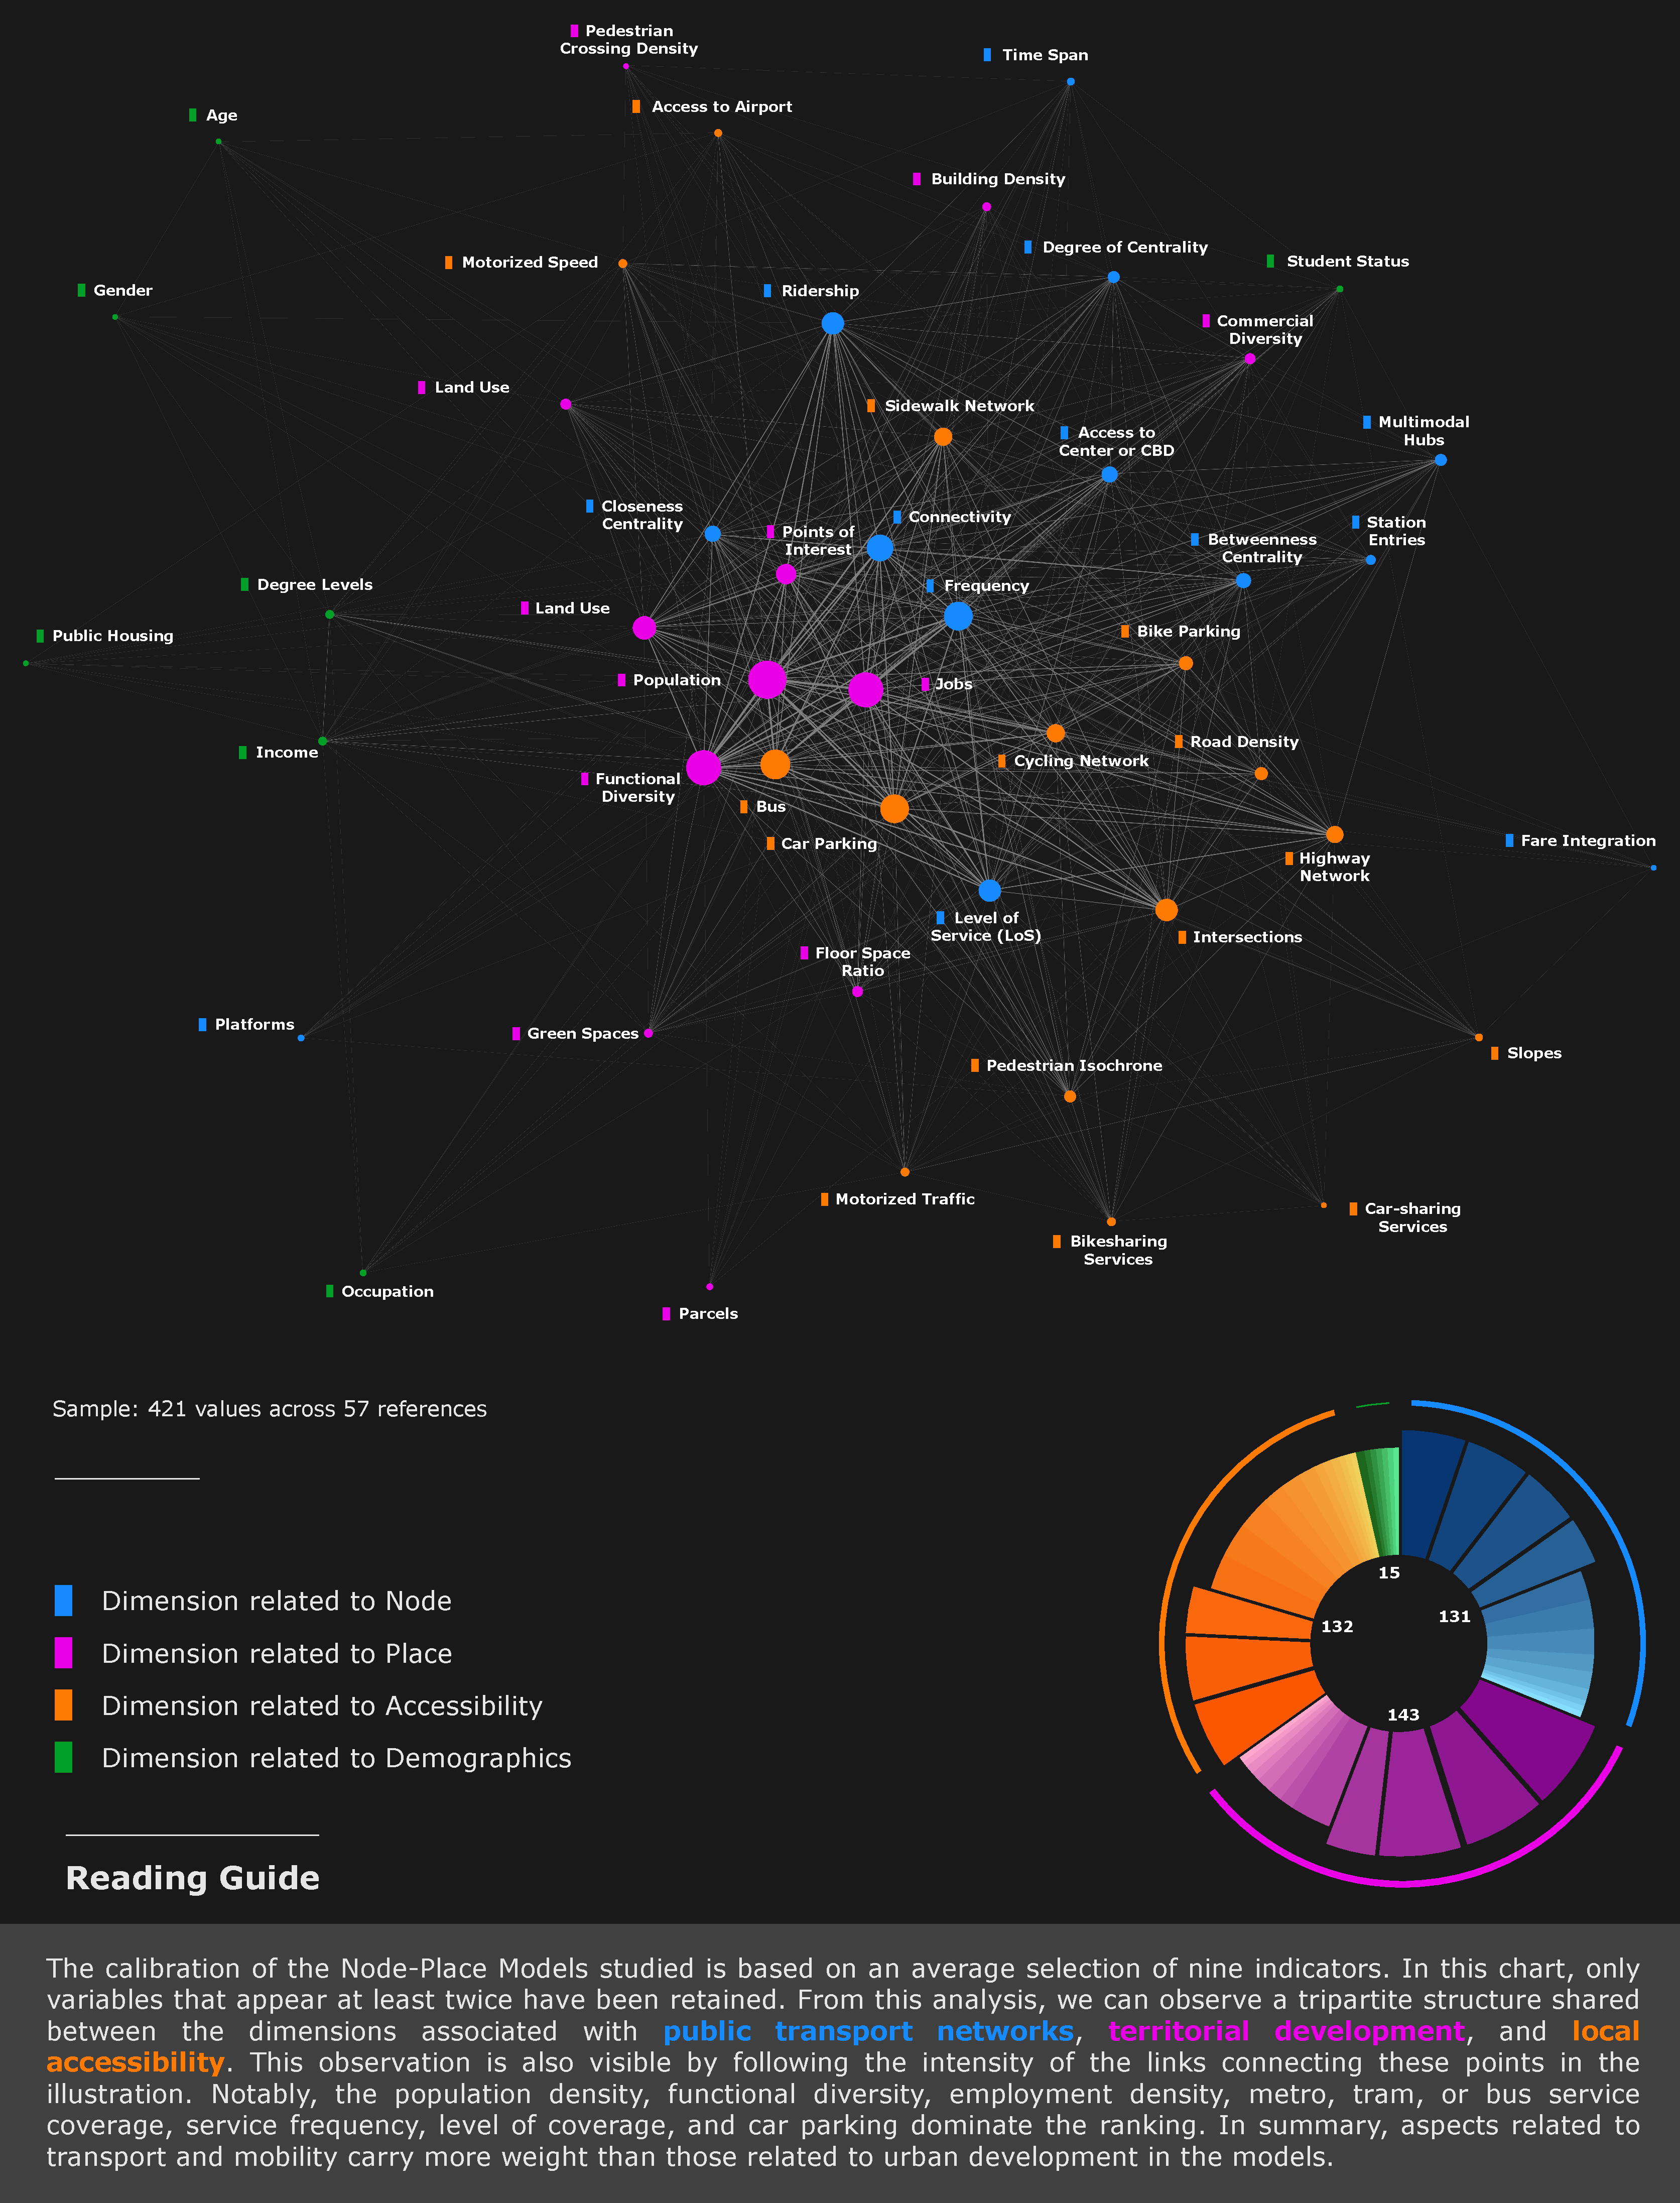
\includegraphics[width=1\columnwidth]{src/Figures/Chap-6/EN_NPART_Litterature_indicateurs.pdf}}
        \vspace{5pt}
        \begin{flushleft}\scriptsize{
        Note: indicators used in the same study are connected by links. The thickness of the links reflects the frequency of joint use of the indicators.
        }\end{flushleft}
        \begin{flushright}\scriptsize{
        Realization: \textcolor{blue}{Dylan Moinse (2024)}
        \\
        Authors: \acrshort{NPART} Research Project
        }\end{flushright}
    \end{figure}

    % Recorded Indicators
Among the 57 studies detailing the parameters defined in the development of their \acrshort{NPM}, we identified 49 indicators with at least 2 occurrences, which we classified into 4 dimensions: \Commas{public transport service,} \Commas{urban development,} \Commas{local accessibility,} and \Commas{socio-demographic characteristics of populations.} In total, 421 occurrences of indicators were recorded, corresponding to an average selection of 9 indicators per model studied. More specifically, as shown in \hyperref[fig-chap6:litterature-indicateurs]{Figure~\ref{fig-chap6:litterature-indicateurs}} (page~\pageref{fig-chap6:litterature-indicateurs}), 13 variables are present in the first dimension, representing 131 occurrences; 12 variables in the second dimension, representing 143 occurrences; 15 variables in the third dimension, representing 132 occurrences; and 7 variables in the last dimension, representing 15 occurrences. This analysis reveals a tripartite distribution of indicators across dimensions related to public transport provision, the degree of urban development, and the quality of public spaces combined with local accessibility. This finding aligns with the analysis by \textcolor{blue}{\textcite[42]{lyu_developing_2016}}\index{Lyu, Guowei|pagebf}\index{Bertolini, Luca|pagebf}\index{Pfeffer, Karin|pagebf}, who identified, based on a systematic literature review, the presence of 94 indicators, of which 24 focus on the \Commas{transport} aspect, 53 on \Commas{urban development,} and 17 on \Commas{\gls{design}.}%%Translated%%

% Main criteria in the literature
The most frequently used criteria include population density (31 occurrences) and employment density (28 occurrences), functional diversity (28 occurrences), urban public transportation accessibility (23 occurrences), mobility service frequency (22 occurrences), level of service in terms of the number of accessible stations within a given time-distance (22 occurrences), car parking availability (22 occurrences), and network connectivity expressed in terms of the number of directions accessible from a station (20 occurrences). By examining the intensity of the links between these indicators in \hyperref[fig-chap6:litterature-indicateurs]{Figure~\ref{fig-chap6:litterature-indicateurs}} (page~\pageref{fig-chap6:litterature-indicateurs}), we observe that the most frequent connections are between population density on the one hand, and employment density (26 links), functional diversity (23 links), car parking (21 links), and the presence of urban public transport systems (21 links) on the other hand, as well as between employment density and functional diversity (20 links).%%Translated%%

% Research recommendations and transition
Despite the identification of a multitude of models adapted to specific research objectives and geographical contexts, \textcolor{blue}{\textcite[394]{ibrahim_planning_2022}}\index{Ibrahim, Sara|pagebf}\index{Ayad, Hany|pagebf}\index{Saadallah, Dina|pagebf} argue that the literature shows a gap in the quantitative measurement of the \acrshort{TOD} potential. Moreover, \textcolor{blue}{\textcite[10-12]{olaru_place_2019}}\index{Olaru, Doina|pagebf}\index{Moncrieff, Simon|pagebf}\index{McCarney, Gary|pagebf}\index{Sun, Yuchao|pagebf}\index{Reed, Tristan|pagebf}\index{Pattison, Cate|pagebf}\index{Smith, Brett|pagebf}\index{Biermann, Sharon|pagebf} recommend integrating mobility solutions related to the \Commas{first and last miles,} which have not received sufficient attention in existing \acrshort{NPM} models. They also suggest expanding the scope of analysis to a broader station area or \Commas{secondary area,} as mentioned by \textcolor{blue}{\textcite[280]{li_transit_2019}}\index{Li, Zekun|pagebf}\index{Han, Zixuan|pagebf}\index{Xin, Jing|pagebf}\index{Luo, Xin|pagebf}\index{Su, Shiliang|pagebf}\index{Weng, Min|pagebf}. On the other hand, \textcolor{blue}{\textcite[80]{robillard_transit-oriented_2024}}\index{Robillard, Arianne|pagebf}\index{Boisjoly, Geneviève|pagebf}\index{Lierop, Dea van|pagebf} as well as \textcolor{blue}{\textcite[120]{nigro_land_2019}}\index{Nigro, Antonio|pagebf}\index{Bertolini, Luca|pagebf}\index{Moccia, Francesco Domenico|pagebf} emphasize the importance of distinguishing between pedestrian and cycling environments around train stations, an aspect often overlooked in the context of the model and \acrshort{TOD} more broadly. Following these recommendations, along with those of \textcolor{blue}{\textcite[9]{motieyan_development_2018}}\index{Motieyan, Hamid|pagebf}\index{Mesgari, Mohammad Saadi|pagebf} who propose developing a model that considers spatial and temporal dynamics, we have developed an \acrshort{NPM} model enriched with suggestions from previous studies, while refocusing our main research. We have therefore opted for the calculation of an extended model aimed at covering the entire rail network, in order to maintain coherence as recommended by \textcolor{blue}{\autocite[58]{chorus_application_2011}}\index{Chorus, Paul|pagebf}\index{Bertolini, Luca|pagebf}, and on a large regional scale, in line with the recommendations of \textcolor{blue}{\textcite[643]{wei_classifying_2023}}\index{Wei, Sheng|pagebf}\index{Wang, Lei|pagebf}. These concerns expressed in the literature form the subject of the following section, in which we present the defined indicator grid, with the aim of extending and adjusting this advanced model to our research problem.%%Translated%%

% ___________________________________________
% 6.2.
\newpage
\needspace{1\baselineskip} % Reserve space
\sectionheader{Grid of Synthetic Indicators Integrated into the Modeling}
\section{Selection of Synthetic Indicators Quantifying and Characterizing the Four Dimensions of the Modeling
    \label{chap6:selection-indicateurs}
    }

% Introduction
The exploration of the scientific literature regarding the \acrshort{NPM} illustrates how this quantitative approach evolves as research progresses. This technical framework, whose main objective is to classify nodes and their environment in order to detect \acrshort{TOD} potential, continues to improve by gradually integrating new dimensions related to the concept of urban planning, enriched by increasingly detailed knowledge. Although new indicators are proposed and integrated into the developed models, our first section identified some inherent gaps associated with our \acrshort{SLR} on \acrshort{B-TOD}. These limitations concern, on the one hand, the delimitation of restricted geographic areas around station neighborhoods, based on a narrow conception of combined walking. This research practice also supports the almost total absence of models that take into account the contribution of cycling and micromobility. On the other hand, at a larger scale, the defined geographic areas are often limited to a municipality or an agglomeration. Furthermore, the lack of case studies located in France, despite the richness of open databases, encourages us to conduct such an investigation on this territory, in order to identify similarities or even national or local specificities.%%Translated%%

% Innovations
Building on this observation, we adopted an innovative approach by choosing to explore an uncharted area, while integrating the most recent contributions related to the \acrshort{NPM}. This includes a variety of indicators introduced in the latest published models, as well as original parameters focusing on the still under-documented integration of light individual mobility. In other words, the modeling we have adopted is based on a revised version of the \acrshort{NPM}, considering the contribution of cycling and micromobility. This approach aims to determine whether nuances emerge in comparison with combined walking, within the expanded framework of a region.%%Translated%%

% Choice and originality of the dimensions
In this regard, the definition of our \acrshort{NPM} derives its originality from the integration of two innovative dimensions. On the one hand, we ensured the inclusion of the links established between the station-object and the urban-object in the form of public spaces. On the other hand, the aim is to bring these themes into dialogue with mobility demand, expressed through the dynamic ridership of public transport stations. Thus, four dimensions structure the modeling we have chosen to name \acrfull{NPART}. For each indicator used, \hyperref[annexes:npart-node]{Appendices~\ref{annexes:npart-node}, \ref{annexes:npart-place-pi}, \ref{annexes:npart-place-ci}, \ref{annexes:npart-accessibility-pi} and~\ref{annexes:npart-accessibility-ci}} (pages~\pageref{annexes:npart-node}, \pageref{annexes:npart-place-pi}, \pageref{annexes:npart-place-ci}, \pageref{annexes:npart-accessibility-pi} and~\pageref{annexes:npart-accessibility-ci}) provide information on their statistical distribution, with the aim of informing the upcoming typological approach, highlighting the variance that differentiates stations.%%Translated%%

% Details of the dimensions + announcement of the outline
Firstly, the two traditional components of the \acrshort{NPM} structure our model: (i) the configuration and quality of service of the rail network represent the \textsl{node} axis of the planning concept (see the \hyperref[chap6:methodologie-indicateurs-node]{\textsl{Transit} section}, page~\pageref{chap6:methodologie-indicateurs-node}), (ii) combined with the territorial arrangements \textsl{around} the railway connection points, which correspond to the \textsl{place} axis (see the \hyperref[chap6:methodologie-indicateurs-place]{\textsl{Development} section}, page~\pageref{chap6:methodologie-indicateurs-place}). Secondly, the expansion of this geostatistical approach is reflected in (iii) the integration of the quality of public spaces and local accessibility, which question the level of urban development \textsl{connected} to these stations, and thus make up the \textsl{accessibility} axis (see the \hyperref[chap6:methodologie-indicateurs-accessibility]{\textsl{Oriented} section}, page~\pageref{chap6:methodologie-indicateurs-accessibility}). Additionally, (iv) passenger flows are analyzed from a temporal perspective and embody the final axis associated with \textsl{ridership per time} (see the \hyperref[chap6:methodologie-indicateurs-frequentation]{\textsl{Demand} section}, page~\pageref{chap6:methodologie-indicateurs-frequentation}). These four dimensions, detailed in the following subsections, thus form the foundation of our \acrshort{NPART} model. This model is part of a broader effort to redefine the framework of \acrshort{M-TOD}, which is the central focus of this doctoral research.%%Translated%%

% 6.2.1.
\needspace{1\baselineskip} % Reserve space
\subsection{Quality of Rail Service (\textsl{Node})
    \label{chap6:methodologie-indicateurs-node}
    }

% Node categories
The first dimension, related to \Commas{rail service quality,} is divided into four categories: \Commas{service level,} \Commas{system performance,} \Commas{network metrics} from a graph perspective, and \Commas{accessibility to urban centers} in Lille and Paris, as presented in \hyperref[table-chap6:indicateurs-node]{Table~\ref{table-chap6:indicateurs-node}} (page~\pageref{table-chap6:indicateurs-node}). The goal of this first dimension, in line with the original \acrshort{NPM}, is to represent the rail service, denoted by \(N\), in the region, by examining its various aspects structured around sixteen key indicators. It is worth noting that, unlike the other three dimensions, the values of each of the synthetic indicators are similar for the four types of geographic areas studied (\(PI\), \(PB\), \(CI\), and \(CB\)).%%Translated%%

% Justification of Node Indicators
This first category, pertaining to the \textsl{Transit} component of \textsl{Transit-Oriented Development}, aims to comprehensively assess the service quality provided by the rail infrastructure. It has been established that the frequency of public transport networks significantly influences station ridership \textcolor{blue}{\autocite[79]{sung_transit-oriented_2011}}\index{Sung, Hyungun|pagebf}\index{Oh, Ju-Taek|pagebf}. Similarly, \textcolor{blue}{\textcite[63]{kashfi_effects_2015}}\index{Kashfi, Syeed Anta|pagebf}\index{Bunker, Jonathan~M.|pagebf}\index{Yigitcanlar, Tan|pagebf} emphasize that service intensity and operational hours contribute to increased ridership. In our modeling framework, we have therefore quantified the service level by defining the frequency of \acrshort{HST} and \acrshort{TER} networks (\(N_{1}\), \(N_{2}\), \(N_{3}\), and \(N_{4}\)), as well as operational hours (\(N_{5}\) and \(N_{6}\)). We also considered system performance, including commercial speed (\(N_{7}\)), which impacts passenger volumes \textcolor{blue}{\autocite[149-201]{vuchic_urban_2007}}\index{Vuchic, Vukan~R.|pagebf}, and the number of directions served (\(N_{8}\)), identified as a key indicator in various \acrshort{NPM} models for station ridership \textcolor{blue}{\autocite[9]{cao_coordination_2020}}\index{Cao, Zhejing|pagebf}\index{Asakura, Yasuo|pagebf}\index{Tan, Zongbo|pagebf}. We explored the network structure through graph analysis, evaluating aspects such as degree centrality (\(N_{9}\)) and closeness centrality (\(N_{11}\)), which, according to \textcolor{blue}{\textcite[14]{shi_exploring_2018}}\index{Shi, Zhuangbin|pagebf}\index{Zhang, Ning|pagebf}\index{Liu, Yang,|pagebf}\index{Xu, Wei|pagebf}, play a key role in station attractiveness, as well as intermediary centrality (\(N_{10}\)), which is associated with increased passenger numbers \textcolor{blue}{\autocite[339]{jang_influence_2022}}\index{Jang, Seongman|pagebf}\index{An, Youngsoo|pagebf}. Finally, the last branch examines accessibility to urban centers, focusing on distances to urban hubs (\(N_{13}\), \(N_{14}\), \(N_{15}\), and \(N_{16}\)), which are inversely correlated with station attractiveness \textcolor{blue}{\autocites[8]{liu_how_2016}[241]{kuby_factors_2004}}\index{Liu, Chao|pagebf}\index{Erdoğan, Sevgi|pagebf}\index{Ma, Ting|pagebf}\index{Ducca, Frederick~W.|pagebf}\index{Kuby, Michael|pagebf}\index{Barranda, Anthony|pagebf}\index{Upchurch, Christopher|pagebf}.%%Translated%%

    % Tableau grille d'indicateurs (node)
% Table indicator grid (node)
%%Translated%%
    \begin{table}[h!]
    \centering
    \renewcommand{\arraystretch}{1.5}
    \resizebox{\columnwidth}{!}{
    \begin{tabular}{p{0.43\columnwidth}p{0.08\columnwidth}p{0.49\columnwidth}}
        %\hline
    \rule{0pt}{15pt} \small{\textbf{\textcolor{blue}{Category}}} & \small{\textbf{\textcolor{blue}{ID}}} & \small{\textbf{\textcolor{blue}{Indicator}}}\\
        \hline
    \multirow{8.5}{*}{\textbf{Service Level}} & \small{\multirow{1.5}{*}{\(N_{1}\)}} & \small{Daily frequency of \acrshort{HST} lines, on weekdays}\\
& \small{\multirow{1.5}{*}{\(N_{2}\)}} & \small{Daily frequency of \acrshort{HST} lines, on Saturdays and Sundays}\\
& \small{\multirow{1.5}{*}{\(N_{3}\)}} & \small{Daily frequency of \acrshort{TER} lines, on weekdays}\\
& \small{\multirow{1.5}{*}{\(N_{4}\)}} & \small{Daily frequency of \acrshort{TER} lines, on Saturdays and Sundays}\\
& \small{\(N_{5}\)} & \small{Time span, on weekdays}\\
& \small{\(N_{6}\)} & \small{Time span, on Saturdays and Sundays}\\
        \hdashline
    \multirow{2}{*}{\textbf{System Performance}} & \small{\(N_{7}\)} & \small{Commercial speed}\\
& \small{\(N_{8}\)} & \small{Number of directions served}\\
        \hdashline
    \multirow{3}{*}{\textbf{Network Metric}} & \small{\(N_{9}\)} & \small{Degree of centrality}\\
& \small{\(N_{10}\)} & \small{Intermediary centrality}\\
& \small{\(N_{11}\)} & \small{Proximity centrality}\\
        \hdashline
    \multirow{8}{*}{\textbf{Accessibility to Centralities}} & \small{\multirow{1.5}{*}{\(N_{12}\)}} & \small{Number of stations accessible within one hour}\\
& \small{\multirow{1.5}{*}{\(N_{13}\)}} & \small{Number of stations to access the urban center of Lille (Euralille hub)}\\
& \small{\multirow{1.5}{*}{\(N_{14}\)}} & \small{Travel time to access the urban center of Lille (Euralille hub)}\\
& \small{\multirow{1.5}{*}{\(N_{15}\)}} & \small{Number of stations to access the urban center of Paris (Châtelet hub)}\\
& \small{\multirow{1.5}{*}{\(N_{16}\)}} & \small{Number of stations to access the urban center of Paris (Châtelet hub)}\\
        \hline
        \end{tabular}}
    \caption{Indicator grid grouped within the dimension related to \Commas{rail service quality} (\textsl{node}).}
    \label{table-chap6:indicateurs-node}
        \vspace{5pt}
        \begin{flushleft}\scriptsize{
        \textcolor{blue}{Reading Guide:} Sixteen indicators are grouped within the dimension \(N\). 
        }\end{flushleft}
        \begin{flushright}\scriptsize{
        Realization: \textcolor{blue}{Dylan Moinse (2024)}
        \\
        Authors: \acrshort{NPART} Research Project
        }\end{flushright}
        \end{table}%%Rédigé%%

% 6.2.1.1.
\needspace{1\baselineskip} % Reserve space
\subsubsection*{Network Service Level \(N_{1} - N_{6}\)
    \label{chap6:indicateurs-node-niveau-service}
    }

% \Commas{Service level} category
Regarding the \Commas{service level} of the intercity public transport network, we deemed it relevant to integrate six factors addressing two distinct aspects\footnote{~
    To do this, we used the static datasets \acrfull{GTFS} provided by \textcolor{blue}{\textcite{sncf_reseau_2024}}. The first dataset covers the period from March 18 to April 12, 2024, for the \acrshort{HST}, while the second spans from March 23 to April 21, 2024. Based on graph representations, we determined the average frequency of \acrshort{HST} lines on weekdays (over 20 days) and weekends (over 7 days), as well as \acrshort{TER} lines on weekdays (over 25 days) and weekends (over 10 days), also calculating the average operational hours over 5 days and 2 days, respectively. The unit of measurement used is the number of trains per day for frequency and the number of hours and minutes the lines are in service daily for operational hours.
}. The first aspect involves examining the daily frequency of the different lines by differentiating the types of system: on the one hand, \acrshort{HST} lines (\(N_{1}\) and \(N_{2}\)) and, on the other hand, regional lines such as \acrshort{TER} and \acrfull{TERGV} (\(N_{3}\) and \(N_{4}\)). This analysis is conducted by taking weekdays into account, distinguishing working days from weekends. The second aspect concerns the operational hours of mobility services, on weekdays (\(N_{5}\)) and weekends (\(N_{6}\)).%%Translated%%

% Descriptive statistics
The average frequency of the 318 stations on the \acrshort{HST} network is 0.76 trains per weekday and 0.65 trains on Saturdays and Sundays. However, this average rises to 14.29 and 12.23 daily trains, respectively, when considering only the 17 stations served by the high-speed rail network. For the regional rail network, the average frequency of the 318 stations is 31.50 trains per weekday and 13.30 trains per weekend day. Regarding operating hours, the rail lines are generally in service for 14 hours and 47 minutes on weekdays and 12 hours and 36 minutes on weekends\footnote{~
    \textsl{Frequency} (\(N_{1} - N_{4}\)): as an example, the multimodal exchange hub \textsl{Euraflandres} stands out with a frequency of 91.95 \acrshort{HST} trains on weekdays and 82.57 \acrshort{HST} trains on weekends, and 512.92 and 228.30 \acrshort{TER} and \acrshort{TERGV} trains daily, respectively.
    \\
    \textsl{Operating hours} (\(N_{5} - N_{6}\)): the Amiens station ranks first with service durations of 19 hours and 31 minutes on weekdays and 18 hours and 49 minutes on weekends.
}%%Translated%%

% 6.2.1.2.
\needspace{1\baselineskip} % Reserve space
\subsubsection*{System Performance \(N_{7} - N_{8}\)
    \label{chap6:indicateurs-node-performance}
    }

% \Commas{Performance} category
The \Commas{system performance} is structured around two main indicators: the commercial speed of the rail network (\(N_{7}\)) and the number of directions served at the examined stations (\(N_{8}\))\footnote{~
    For these two variables, we selected Tuesday, March 19, 2024, to aggregate all recorded speeds and the directions offered at each station, using graph representations. For speed calculations, we determined the average speed of each railway line serving the stations, and then retained the highest average speed for each station.
}. Thus, the average speed at the 318 stations is 69.68 kilometers per hour, rising to 137.97 kilometers per hour at the 17 stations served by the \acrshort{HST} network, and 65.83 kilometers per hour at stations exclusively connected to the \acrshort{TER} network. Regarding the number of directions offered by the stations, the average is 3.35 different destinations per station\footnote{~
    \textsl{Commercial speed and number of directions} (\(N_{7} - N_{8}\)): the station with the fastest line and the most directions offered is the \textsl{Euraflandres hub}, with an average speed of 236.75 kilometers per hour and 48 different destinations.
}.%%Translated%%

% 6.2.1.3.
\needspace{1\baselineskip} % Reserve space
\subsubsection*{Network Metrics \(N_{9} - N_{11}\)
    \label{chap6:indicateurs-node-metrique}
    }

% \Commas{Metrics} category
The \Commas{network metrics} are structured around three synthetic indicators: degree centrality (\(N_{9}\)), betweenness centrality (\(N_{10}\)), and closeness centrality (\(N_{11}\))\footnote{~
    Degree centrality measures the number of direct connections a node has with other nodes in a network. The more connections a node has, the higher its degree centrality. By direct connections, we mean the number of stations reached by rail services, without transfers, from the starting station.
    \\
    Betweenness centrality quantifies how often a node appears in the shortest paths between other nodes. A node with high betweenness centrality plays a crucial role as a mediator in a network.
    \\
    Closeness centrality measures how close a node is to all other nodes in a network. It is defined as the inverse of the sum of the shortest distances between a node and all other nodes.
}. These three main measures from graph theory allow us to assess the strategic position of stations in the rail network\footnote{~
    For this analysis, we also selected Tuesday, March 19, 2024, as the baseline working day to study all the scheduled rail flows for that day.
}. The averages for degree centrality, betweenness centrality, and closeness centrality for the 318 stations in the region are 0.001, 0.092, and 0.001, respectively\footnote{~
    \textsl{Position in the network} (\(N_{9} - N_{11}\)): the station with the highest metric values is once again the \textsl{Euraflandres hub}, with a degree centrality of 0.008, betweenness centrality of 0.246, and closeness centrality of 0.102.
}.%%Translated%%

% 6.2.1.4.
\needspace{1\baselineskip} % Reserve space
\subsubsection*{Accessibility to Urban Centers \(N_{12} - N_{16}\)
    \label{chap6:indicateurs-node-accessibilite-centralites}
    }

    % Category \Commas{accessibility to centralities}
The last aspect corresponds to the \Commas{accessibility to urban centralities} and includes five indicators: the number of stations accessible within one hour of travel (\(N_{12}\)), the number of stations and the time-distance required to reach respectively the Euralille hub, located in the center of Lille (\(N_{13}\) and \(N_{14}\)), and the Châtelet hub, located in the center of Paris (\(N_{15}\) and \(N_{16}\)). Since this last category focuses on the distance to attractive urban hubs, the values obtained, whether for \(N_{13}\), \(N_{14}\), \(N_{15}\), or \(N_{16}\), are inverted in the model in order to rank the nodes based on their proximity to Lille and Paris\footnote{~
    The time budget allocated was determined based on the public survey conducted by the \textcolor{blue}{\textcite{ministere_de_la_transition_ecologique_et_de_la_cohesion_des_territoires_mobilite_2023}}, which indicates that a \Commas{local or long-distance} trip in France lasts an average of 41 minutes in 2019. This data was cross-referenced with our empirical material, which suggests an average of one hour of travel by \acrshort{HST} and \acrshort{TER} in the region. Similarly to the previous analysis, we selected Tuesday, March 19, 2024, between 5:00 AM and 11:00 PM, to study accessibility to other stations in the national network. Regarding accessibility to the urban centralities of Euralille and Châtelet, we analyzed the flows from March 18 to March 24, 2024, covering a full week, and then kept the lowest values for each station.
}.%%Translated%%

    % Descriptive statistics for stations within 1 hour
For accessibility to other stations within a given time, the average number of stations accessible within 1 hour is approximately 1.99, compared to 4.58 stations for the 17 stations connected to the high-speed rail network. For access to the urban center of Lille, the average number of stations required to access it is 4.63, with an average time-distance of 1 hour and 10 minutes. Accessibility to the urban center of Paris shows an average of 5.83 stations required to access it, with an average time-distance of 1 hour and 50 minutes. Nine stations in the region have direct train access, without intermediate stops, although requiring a transfer at Gare du Nord to reach the urban center of Paris. Among these stations, only two are served by the \acrshort{HST}: those in Arras and \textsl{Euraflandres}\footnote{~
    \textsl{Access to other stations} (\(N_{12}\)): the \textsl{Euraflandres hub} remains at the top of the ranking with an average of 15.44 stations accessible within one hour.
    \\
    \textsl{Access to Lille} (\(N_{13} - N_{14}\)): excluding the multimodal exchange hub relevant to the indicators related to distances to Euralille, 24 stations have a direct connection without intermediate stops to the urban center of Lille. Apart from the stations in the \acrfull{MEL}, regionally significant stations such as those in Arras, Calais-Fréthun, Douai, Dunkirk, Orchies, Templeuve, TGV Haute Picardie, and Valenciennes are part of these direct connections. Additionally, 37 stations are connected within 20 minutes of Euralille, mainly within the \acrshort{MEL}, with the exception of the stations in Douai, Landas, Libercourt, Nieppe, Nomain, Orchies, Ostricourt, and Phalempin.
    \\
    \textsl{Access to Paris} (\(N_{15} - N_{16}\)): in terms of time-distance, the station at Orry-la-Ville-Coye records the shortest score with 28 minutes, followed by Chantilly-Gouvieux with 33 minutes, and Creil with 36 minutes, these three stations being on the border of Île-de-France and connected to the D line of the \acrfull{RER}.
}.%%Translated%%

    % 6.2.1.5.
    \needspace{1\baselineskip} % Reserve space
\subsubsection*{Originality of the Dimension related to the Node
    \label{chap6:indicateurs-node-originalite}
    }

    % Introduction
By proposing these sixteen indicators for the dimension related to rail supply, our model draws inspiration from previous \acrshort{NPM} models while refining them. This first dimension, focusing on infrastructure and regional mobility service, aims to address the three main challenges faced by the development of public transport accessibility models: system performance, the configuration of the public transport network, and access to various destinations \textcolor{blue}{\autocite[744]{malekzadeh_review_2020}}\index{Malekzadeh, Ali|pagebf}\index{Chung, Edward|pagebf}.%%Translated%%

    % System performance 1
From the perspective of rail service quality, we first sought to expand the temporal scope of the statistical analysis by projecting more complex graphs that go beyond the simple consideration of a single time interval or a single day, unlike nearly all of the studies reviewed. Indeed, most of these studies calculate these variables from a typical day, usually a Tuesday, or even from a single time slot, most often during peak hours. Although frequency is one of the most commonly used indicators, the originality of our model lies in the distinction between different public transport systems, as well as the separation between weekdays and weekends. This concern for differentiation reflects the models developed by \textcolor{blue}{\textcite[149]{ivan_evaluation_2012}}\index{Ivan, Igor|pagebf}\index{Boruta, Tomáš|pagebf}\index{Horak, Jiri|pagebf} who isolated the frequency of trains from that of suburban trains, trams, and buses, as well as by \textcolor{blue}{\textcite[117]{nigro_land_2019}}\index{Nigro, Antonio|pagebf}\index{Bertolini, Luca|pagebf}\index{Moccia, Francesco Domenico|pagebf}, whose frequency was assessed according to work and vacation periods.%%Translated%%

    % System performance 2
Similarly, the number of stations accessible within a given time-distance has been widely incorporated into \acrshort{NPM} models. However, we chose to broaden the time interval, which is typically limited to twenty minutes and seems poorly suited to a regional rail system. Regarding the time range between the first and last train in service, only the model from \textcolor{blue}{Freke} \textcolor{blue}{\textcite[132]{caset_planning_2019}}\index{Caset, Freke|pagebf}’s doctoral thesis considers this aspect. The issue of train commercial speed has been addressed by improving the work of \textcolor{blue}{\textcite[271]{debrezion_modelling_2009}}\index{Debrezion, Ghebreegziabiher|pagebf}\index{Pels, Eric|pagebf}\index{Rietveld, Piet|pagebf} and \textcolor{blue}{\textcite[6]{zheng_classifying_2023}}\index{Zheng, Lingwei|pagebf}\index{Austwick, Martin Zaltz|pagebf}, who focused on the theoretical speed of trains. To this end, we chose to calculate the operational average speed on the commercial network, rather than using the theoretical speed.%%Translated%%

    % Network structure
While the quality of rail service is generally well accounted for in previous models, it appears that measures related to the network configuration are rarely exploited in an adequate manner \textcolor{blue}{\autocite[72-74]{papa_accessibility_2015}}\index{Papa, Enrica|pagebf}\index{Bertolini, Luca|pagebf}. However, as demonstrated by \textcolor{blue}{\textcite[8]{dou_integrating_2021}}\index{Dou, Mingxuan|pagebf}\index{Wang, Yandong|pagebf}\index{Dong, Shihai|pagebf}, who introduced this concept in a third dimension called \Commas{\textsl{Node-Place-Network}} (NPN), it proves effective for better understanding the performance of the network under study. With this in mind, we have incorporated three indicators: centrality degree, betweenness centrality, and proximity centrality, which, according to our observations, have not yet been analyzed together in existing studies.%%Translated%%

    % 6.2.2.
    \needspace{1\baselineskip} % Reserve space
\subsection{Degree of Urban Development (\textsl{Place})
    \label{chap6:methodologie-indicateurs-place}
    }

    % Categories place
The second dimension, related to the \Commas{degree of urban development}, is divided into five categories: \Commas{density}, \Commas{functional diversity}, \Commas{attractive places}, \Commas{land value}, and \Commas{social stratification}, as presented in \hyperref[table-chap6:indicateurs-place]{Table~\ref{table-chap6:indicateurs-place}} (page~\pageref{table-chap6:indicateurs-place}). The objective of this category, also in line with the original \acrshort{NPM}, is to measure urban forms, facilities, and the attractiveness of areas, as well as the sociological profile of resident populations, denoted by \(P\), by examining its various aspects structured around thirteen key indicators.%%Translated%%

    % Tableau grille d'indicateurs (place)
% Table indicator grid (place)
%%Translated%%
    \begin{table}[h!]
    \centering
    \renewcommand{\arraystretch}{1.5}
    \resizebox{\columnwidth}{!}{
    \begin{tabular}{p{0.43\columnwidth}p{0.08\columnwidth}p{0.49\columnwidth}}
        %\hline
    \rule{0pt}{15pt} \small{\textbf{\textcolor{blue}{Category}}} & \small{\textbf{\textcolor{blue}{ID}}} & \small{\textbf{\textcolor{blue}{Indicator}}}\\
        \hline
    \multirow{2}{*}{\textbf{Density}} & \small{\(P_{1}\)} & \small{Population density}\\
& \small{\(P_{2}\)} & \small{Employment density}\\
        \hdashline
    \multirow{5.5}{*}{\textbf{Functional Diversity}} & \small{\multirow{1.5}{*}{\(P_{3}\)}} & \small{Residential-dominant land use}\\
& \small{\multirow{1.5}{*}{\(P_{4}\)}} & \small{Commercial and public service-dominant land use}\\
& \small{\multirow{1.5}{*}{\(P_{5}\)}} & \small{Office and industrial-dominant land use}\\
& \small{\multirow{1}{*}{\(P_{6}\)}} & \small{Green space-dominant land use}\\
        \hdashline
    \multirow{3}{*}{\textbf{Attraction Locations}} & \small{\(P_{7}\)} & \small{Proximity points of interest (\acrshort{POIs})}\\
& \small{\multirow{1}{*}{\(P_{8}\)}} & \small{Intermediate points of interest (\acrshort{POIs})}\\
& \small{\(P_{9}\)} & \small{Superior points of interest (\acrshort{POIs})}\\
        \hdashline
    \multirow{2.5}{*}{\textbf{Land Value}} & \small{\(P_{10}\)} & \small{Land value of residential properties}\\
& \small{\multirow{1.5}{*}{\(P_{11}\)}} & \small{Land value of industrial, commercial, and office properties}\\
        \hdashline
    \multirow{2}{*}{\textbf{Social Stratification}} & \small{\(P_{12}\)} & \small{Proportion of social housing}\\
& \small{\(P_{13}\)} & \small{Average household income}\\
        \hline
        \end{tabular}}
    \caption{Indicator grid grouped within the dimension related to \Commas{urban development degree} (\textsl{place}).}
    \label{table-chap6:indicateurs-place}
        \vspace{5pt}
        \begin{flushleft}\scriptsize{
        \textcolor{blue}{Reading Guide:} Thirteen indicators are grouped within the dimension \(P\). 
        }\end{flushleft}
        \begin{flushright}\scriptsize{
        Realization: \textcolor{blue}{Dylan Moinse (2024)}
        \\
        Authors: \acrshort{NPART} Research Project
        }\end{flushright}
        \end{table}%%Rédigé%%

    % 6.2.2.1.
    \needspace{1\baselineskip} % Reserve space
\subsubsection*{Population and Employment Density \(P_{1} - P_{2}\)
    \label{chap6:indicateurs-place-densite}
    }

    % Category \Commas{density}
Regarding \Commas{density}, it concerns both population density (\(P_{1}\)) and employment density (\(P_{2}\))\footnote{~
    Their measurement relied on two datasets: for the first indicator, the population grid data from 2019, in the form of 200-meter-square tiles, and for the second indicator, the \acrfull{Sirene} data from April 2, 2024, both provided by \textcolor{blue}{\textcite{insee_grille_2021}}. We prioritized the calculation of a stock of residents and jobs rather than their density, in order to obtain a raw measure easily comparable to other indicators. This approach helps avoid the influence of the size of station neighborhoods and thus limits bias in the results. Ultimately, this stock measure can be easily converted into densities.
}. Among the 318 station neighborhoods specific to each geographic perimeter, the average population density, measured in inhabitants per square kilometer, is 2,999.78 at the pedestrian isochrone scale (\(PI\)), 1,576.72 for pedestrian buffer zones (\(PB\)), 1,325.03 for cycling isochrones (\(CI\)), and 773.68 for cycling buffer zones (\(CB\)). The top ten positions in the ranking are held by station neighborhoods from the \acrshort{MEL}. Regarding employment density, stations in the region record an average of 418.95 (\(PI\)), 240.03 (\(PB\)), 190.93 (\(CI\)), and 121.14 (\(CB\)) jobs per square kilometer\footnote{~
    \textsl{Population density} (\(P_{1}\)): in terms of \(PI\), the \textsl{Euraflandres} hub has the highest density, with 12,931.92 inhabitants per square kilometer, while the areas around the Croix l'Allumette station for \(PB\) (10,486.60) and Lezennes for \(CI\) (9,031.43) and \(CB\) (9,018.71) top the list.
    \\
    \textsl{Employment density} (\(P_{2}\)): the areas surrounding stations with the highest employment densities are those in Amiens for \(PI\) (3,498.30) and Lille CHR for \(PB\) (3,423.08), \(CI\) (3,289.78), and \(CB\) (2,804.25).
}.%%Translated%%

    % 6.2.2.2.
    \needspace{1\baselineskip} % Reserve space
\subsubsection*{Functional Diversity \(P_{3} - P_{6}\)
    \label{chap6:indicateurs-place-diversite}
    }
    
    % Category \Commas{functional diversity}
Four aspects define \Commas{functional diversity}, namely residential land use (\(P_{3}\)), commercial and public service-related use (\(P_{4}\)), office and industrial use (\(P_{5}\)), and green spaces (\(P_{6}\))\footnote{~
    These indicators were determined using the reference framework of the \acrfull{OCS2D} for the five departments making up the Hauts-de-France region. This file was published in 2021 by the collaborative geographic platform \textcolor{blue}{\textcite{geo2france_occupation_2021}}\index{Géo2France@\textsl{Géo2France}|pagebf}, set up by the Region.
}. In general, station neighborhoods at the \(PI\) scale show a spatial proportion of residential use of around 41.95\%, compared to 22.83\% (\(PB\)), 21.84\% (\(CI\)), and 12.77\% (\(CB\)). The surface area occupied by commercial and public services reaches 6.61\% (\(PI\)), 4.89\% (\(PB\)), 5.01\% (\(CI\)), and 3.31\% (\(CB\)). Regarding office and industrial activities, the share is 4.66\% (\(PI\)), 4.71\% (\(PB\)), 4.17\% (\(CI\)), and 3.13\% (\(CB\)). Finally, green spaces cover 1.69\% of \(PI\), 1.24\% of \(PB\), 1.26\% of \(CI\), and 0.86\% of \(CB\)\footnote{~
    \textsl{Residential use} (\(P_{3}\)): with a rate of 77.02\%, the areas around Nieppe are the most residential in proportion at the pedestrian isochrone scale, followed by Ronchin at 61.03\%; 58.73\% and 58.20\% for the three other types of geographic perimeters.
    \\
    \textsl{Commercial and public services} (\(P_{4}\)): the station neighborhoods of Poirier Université, with 32.14\% for \(PI\), Chantilly~–~Gouvieux, with 33.42\% and 29.72\% for \(PB\) and \(CI\), as well as Pont de Bois, with 26.76\% for \(CI\), top the list.
    \\
    \textsl{Office and industrial activities} (\(P_{5}\)): the locations in Mont de Terre, with 51.13\%; 28.79\% and 23.31\% for \(PI\), \(CI\), and \(CB\), and in Nesle, with 27.53\% for \(PB\), dominate this category.
    \\
    \textsl{Green spaces} (\(P_{6}\)): the greenest station neighborhoods are those of Quesnoy, with 31.72\% (\(PI\)), and Lens, with 13.67\% (\(PB\)), 9.71\% (\(CI\)), and 9.66\% (\(CB\)).
}.%%Translated%%

    % 6.2.2.3.
    \needspace{1\baselineskip} % Reserve space
\subsubsection*{Attractive Places \(P_{7} - P_{9}\)
    \label{chap6:indicateurs-place-pois}
    }

    % Category \Commas{attractive places}
\Commas{Attractive places} are classified into three distinct categories of \acrfull{POIs}, based on their functions: \Commas{proximity} \acrshort{POIs} (\(P_{7}\)), \Commas{intermediate} \acrshort{POIs} (\(P_{8}\)), and \Commas{superior} \acrshort{POIs} (\(P_{9}\))\footnote{~
    This segmentation follows the three categories defined by \textcolor{blue}{\textcite{insee_base_2021}} in the \acrfull{BPE}, as detailed in the \hyperref[chap5:potentiel-accessibilite-destinations]{section on regional accessibility gains to places of interest~\ref{chap5:potentiel-accessibilite-destinations}} (page~\pageref{chap5:potentiel-accessibilite-destinations}), from \hyperref[chap5:titre]{Chapter~\ref{chap5:titre}} (page~\pageref{chap5:titre}).
}. First, the average number of \Commas{proximity} \acrshort{POIs} is 48.85 for \(PI\), 59.67 for \(PB\), 115.77 for \(CI\), and 134.87 for \(CB\). Second, the average number of \Commas{intermediate} \acrshort{POIs} is 24.96 (\(PI\)), 29.53 (\(PB\)), 53.79 (\(CI\)), and 60.74 (\(CB\)). Finally, \Commas{superior} \acrshort{POIs} have an average of 8.51 (\(PI\)), 10.61 (\(PB\)), 20.79 (\(CI\)), and 23.08 (\(CB\))\footnote{~
    \textsl{Points of interest} (\(P_{7} - P_{9}\)): the \textsl{Euraflandres} station neighborhood offers the greatest number of attractive places, across all categories, with 888; 1,134; 1,747; and 1,778 local services for \(PI\), \(PB\), \(CI\), and \(CB\) respectively, 590; 701; 940; and 957 intermediate services, and 172; 232; 391; and 397 regional interest services.
}.%%Translated%%

    % 6.2.2.4.
    \needspace{1\baselineskip} % Reserve space
\subsubsection*{Land Value \(P_{10} - P_{11}\)
    \label{chap6:indicateurs-place-foncier}
    }
    
    % Category \Commas{land value}
\Commas{Land value} concerns the land value attributed to residential properties (\(P_{10}\)) as well as industrial, commercial, or office spaces (\(P_{11}\))\footnote{~
    To this end, we consolidated the annual databases of the Demande Valeur Foncière (DVF), provided by \textcolor{blue}{\textcite{direction_generale_des_finances_publiques_demandes_2024}}\index{Direction Générale des Finances Publiques@\textsl{Direction Générale des Finances Publiques}|pagebf}, for the period from 2018 to 2023. This merging allowed us to establish an average value, expressed in euros per square meter, for real estate transactions carried out in each station neighborhood during the aforementioned period.
}. The land value of residential properties averages~\euro2,138.47 per square meter in the station neighborhoods designated as \(PI\),~\euro2,132.18 for \(PB\),~\euro2,091.53 for \(CI\), and~\euro2,121.75 for \(CB\). Regarding industrial, commercial, and office properties, the price per square meter ranges from~\euro2,480.26 (\(PI\)),~\euro2,231.09 (\(PB\)),~\euro2,072.25 (\(CI\)), and~\euro1,904.52 (\(CB\))\footnote{~
    \textsl{Residential values} (\(P_{10}\)): for the two types of pedestrian perimeters, the area around Château-Thierry seems to be the most sought after, with a residential value of~\euro12,421.96 (\(PI\)) and~\euro9,905.87 (\(PB\)). The station neighborhoods of Pont-Sainte-Maxence and \textsl{Euraflandres} rank first for \(CI\) and \(CB\) respectively, with land values of~\euro6,162.00 and~\euro6,019.66 per square meter.
    \\
    \textsl{Industrial and commercial values} (\(P_{11}\)): the areas surrounding Pont de Bois stand out in this regard, recording an average land value of~\euro153,313.16 (\(PI\)),~\euro151,861.34 (\(PB\)),~\euro79,550.92 (\(CI\)), and~\euro67,034.70 per square meter (\(CB\)).
}.%%Translated%%

    % 6.2.2.5.
    \needspace{1\baselineskip} % Reserve space
\subsubsection*{Socio-economic Composition of Territories \(P_{12} - P_{13}\)
    \label{chap6:indicateurs-place-sociodemographie}
    }
    
    % Category \Commas{social stratification}
The final aspect of the territorial dimension addresses the \Commas{social stratification} of the studied areas by measuring two indicators related to the socio-economic composition of the locations: the proportion of social housing (\(P_{12}\)) and the annual income of households (\(P_{13}\))\footnote{~
    We used the 2023 \acrfull{RPLS} data provided by \textcolor{blue}{\textcite{ministere_de_la_transition_ecologique_et_de_la_cohesion_des_territoires_repertoire_2024}} to catalog the social housing stock in France. Additionally, we reused the 2019 population grid data from \textcolor{blue}{\textcite{insee_grille_2021}} to determine the average income of each household.
}. Our results indicate that the proportion of social housing varies by geographic area, being 6.53\% in \(PI\), 6.82\% in \(PB\), 7.76\% in \(CI\), and 7.56\% in \(CB\). As for the average household income, it also varies by the studied zones:~\euro4,105.73 for \(PI\),~\euro4,150.90 for \(PB\),~\euro4,217.75 for \(CI\), and~\euro4,277.94 for \(CB\)\footnote{~
    \textsl{Social housing} (\(P_{12}\)): the station neighborhoods of Pont de Bois stand out with the highest concentration of social housing, with 38.58\% (\(PI\)) and 34.37\% (\(PB\)). Regarding the cycling station neighborhoods, Coron de Méricourt shows the highest rates, with 31.06\% (\(CI\)) and 29.96\% (\(CB\)).
    \\
    \textsl{Annual income} (\(P_{13}\)): the most affluent station neighborhoods are those in Jaux, with an annual income of~\euro6,321.52 for \(PI\), Ascq, with~\euro6,199.81 for \(PB\), and Ennevelin, with~\euro6,249.93 and~\euro6,254.31 for the cycling zones.
}.%%Translated%%

% 6.2.2.6.
\needspace{1\baselineskip} % Reserve space
\subsubsection*{Originality of the Dimension in relation to the Location
    \label{chap6:indicateurs-place-originalite}
    }

% Justification literature 1
We have incorporated and developed indicators already present in most \acrshort{NPM} models, such as population and employment density, as well as the functional diversity of territories, alongside new variables. The use of \acrshort{POIs} refers to a relatively small number of studies that have taken into account these urban elements that generate flows \textcolor{blue}{\autocites[82]{robillard_transit-oriented_2024}[2]{zhou_introducing_2023}}\index{Robillard, Arianne|pagebf}\index{Boisjoly, Geneviève|pagebf}\index{Lierop, Dea van|pagebf}\index{Zhou, Mingzhi|pagebf}\index{Zhou, Jiali|pagebf}\index{Zhou, Jiangping|pagebf}\index{Lei, Shuyu|pagebf}\index{Zhao, Zhan|pagebf}. Furthermore, we have chosen to reflect the diversity of \acrshort{POIs}, in line with the recommendations made by \textcolor{blue}{\textcite[7]{zhang_make_2023}}\index{Zhang, Mengyuan|pagebf}\index{Lee, Jinwoo Brian|pagebf}.
%%Translated%%
    


 % Justification literature 2
Although \textcolor{blue}{\textcite{transportation_research_board_of_the_national_academies_transit_2007}}\index{Transportation Research Board@\textsl{Transportation Research Board}|pagebf} recognizes land value as one of the ten key indicators in the construction of an \acrshort{NPM} model, few studies have focused on this issue to date. \textcolor{blue}{\textcite[135]{kim_geographic_2018}}\index{Kim, Hyojin|pagebf}\index{Sultana, Selima|pagebf}\index{Weber, Joe|pagebf} suggest examining property values around train stations to assess urban dynamics, although acquiring such data presents certain challenges. \textcolor{blue}{\textcite[242]{ibrahim_measuring_2023}}\index{Ibrahim, Sara|pagebf}\index{Ayad, Hany|pagebf}\index{Turki, Eslam|pagebf}\index{Saadallah, Dina|pagebf} have succeeded in incorporating the added land value resulting from private investments captured in Alexandria, Egypt.
%%Translated%%
%Toutefois, \textcolor{blue}{\textcite[263]{singh_measuring_2014}}\index{Singh, Yamini Jain|pagebf}\index{Fard, Pedram|pagebf}\index{Zuidgeest, Mark|pagebf}\index{Brussel, Mark|pagebf}\index{Maarseveen, Martin van|pagebf} émettent des doutes sur la nécessité d'améliorer la précision des données statistiques liées aux investissements pour enrichir un tel modèle.%%Rédigé%%

% Justification literature 3
In addition to these considerations, the issue of the supply of social housing, in connection with land tensions, is raised \textcolor{blue}{\autocite[27]{singh_measuring_2015}}\index{Singh, Yamini Jain|pagebf}. This socio-spatial dimension is largely underrepresented in the literature, with the exception of the model undertaken by \textcolor{blue}{\textcite[2]{zhou_introducing_2023}}\index{Zhou, Mingzhi|pagebf}\index{Zhou, Jiali|pagebf}\index{Zhou, Jiangping|pagebf}\index{Lei, Shuyu|pagebf}\index{Zhao, Zhan|pagebf}. Finally, the consideration of household economic resources, particularly income, remains an underutilized indicator in this model, despite being an important factor according to the results derived from the modeling process of \textcolor{blue}{\textcite[3]{cummings_does_2022}}\index{Cummings, Christopher|pagebf}\index{Mahmassani, Hani|pagebf}.
%%Translated%%

% 6.2.3.
\needspace{1\baselineskip} % Reserve space
\subsection{Local Accessibility and Public Space Management (\textsl{Connections})
    \label{chap6:methodologie-indicateurs-accessibility}
    }

% Categories accessibility
The third dimension of this study, referred to as \Commas{local accessibility and public space management,} which is part of the \textsl{Oriented} component of \textsl{Transit-Oriented Development}, focuses on the interactions between urban development and the mobility system. It specifically investigates the scale of links (\textsl{link scale}), exploring the quality of urban planning and its contribution to the qualification of the urban environment \textcolor{blue}{\autocite[294]{zhang_built_2023}}\index{Zhang, Yushan|pagebf}\index{Kasraian, Dena|pagebf}\index{Wesemael, Pieter van|pagebf}. This dimension encompasses the concepts of \Commas{walkability,} \Commas{bikeability,} and \Commas{local connectivity} in relation to urban public transport networks, as well as \Commas{demand management,} focusing on the space allocated to automobiles (see \hyperref[table-chap6:indicateurs-accessibility]{Table~\ref{table-chap6:indicateurs-accessibility}}, page~\pageref{table-chap6:indicateurs-accessibility}). It should be noted that the last category is approached from the perspective of the competitiveness of the car compared to the use of public transport, in line with the principles of \acrshort{TOD}. Thus, the values assigned to the presence of automobiles in urban space are reversed in the modeling: the greater the importance given to the car, the lower the train station district is ranked relative to others. Through this component, denoted \(A\), a total of eleven indicators were integrated to assess the four defined geographical areas (\(PI\), \(PB\), \(CI\), and \(CB\)).
%%Translated%%

    % Tableau grille d'indicateurs (accessibility)
% Table indicator grid (accessibility)
%%Translated%%
    \begin{table}[h!]
    \centering
    \renewcommand{\arraystretch}{1.5}
    \resizebox{\columnwidth}{!}{
    \begin{tabular}{p{0.43\columnwidth}p{0.08\columnwidth}p{0.49\columnwidth}}
        %\hline
    \rule{0pt}{15pt} \small{\textbf{\textcolor{blue}{Category}}} & \small{\textbf{\textcolor{blue}{ID}}} & \small{\textbf{\textcolor{blue}{Indicator}}}\\
        \hline
    \multirow{3.5}{*}{\textbf{Walkability}} & \small{\(A_{1}\)} & \small{Length of the pedestrian network}\\
& \small{\(A_{2}\)} & \small{Intersection density}\\
& \small{\multirow{1.5}{*}{\(A_{3}\)}} & \small{Spatial efficiency rate (walking and cycling isochrones)}\\
        \hdashline
    \multirow{4.5}{*}{\textbf{Cyclability}} & \small{\(A_{4}\)} & \small{Length of the cycling network}\\
& \small{\multirow{1.5}{*}{\(A_{5}\)}} & \small{Capacity of dedicated bicycle parking spaces}\\
& \small{\multirow{1.5}{*}{\(A_{6}\)}} & \small{Bike-sharing fleets (\acrfull{PBS})}\\
        \hdashline
    \multirow{2.5}{*}{\textbf{Local Connectivity}} & \small{\(A_{7}\)} & \small{Metro and tram stops}\\
& \small{\multirow{1.5}{*}{\(A_{8}\)}} & \small{Bus and \acrfull{BRT} stops}\\
        \hdashline
    \multirow{3.5}{*}{\textbf{Demand Management}} & \small{\(A_{9}\)} & \small{Motorized speed limit}\\
& \small{\multirow{1.5}{*}{\(A_{10}\)}} & \small{Surface area of car parking spaces}\\
& \small{\(A_{11}\)} & \small{Motorization rate of households}\\
        \hline
        \end{tabular}}
    \caption{Indicator grid grouped within the dimension related to \Commas{local accessibility and public space management} (\textsl{connectivity}).}
    \label{table-chap6:indicateurs-accessibility}
        \vspace{5pt}
        \begin{flushleft}\scriptsize{
        \textcolor{blue}{Reading Guide:} Eleven indicators are grouped within the dimension \(A\). 
        }\end{flushleft}
        \begin{flushright}\scriptsize{
        Realization: \textcolor{blue}{Dylan Moinse (2024)}
        \\
        Authors: \acrshort{NPART} Research Project
        }\end{flushright}
        \end{table}%%Rédigé%%

% 6.2.3.1.
\needspace{1\baselineskip} % Reserve space
\subsubsection*{Walkability \(A_{1} - A_{3}\)
    \label{chap6:indicateurs-accessibility-marchabilite}
    }

% Category \Commas{walkability}
\Commas{Walkability} is quantified using three indicators: the total length of pedestrian spaces (\(A_{1}\)), the intersection density reflecting the connectivity of the road network (\(A_{2}\)), and the ratio between the area of isochrones and that of buffer zones, which illustrates the actual physical access to the territory (\(A_{3}\))\footnote{~
    Data for these three indicators were extracted from \textsl{OpenStreetMap} on Friday, April 5, 2024.
}.
%%Translated%%

% Descriptive statistics 1
Across all the studied train station districts, we observe that the average length of pedestrian networks is 15.70 kilometers in the walkable isochrones (\(PI\)) and 24.33 kilometers in the corresponding buffer zones (\(PB\)). For areas accessible via light individual mobility, these lengths extend to 72.39 kilometers for the isochrones (\(CI\)) and 103.47 kilometers for the buffer zones (\(CB\)). Regarding intersection density, the analysis reveals an average of 238.60 intersections per square kilometer for \(PI\), compared to 126.27 for \(PB\), 122.05 for \(CI\), and 71.59 for \(CB\). The spatial efficiency rate, which measures the proportion of accessible space (isochrone) relative to theoretically accessible space (buffer zone), shows an average of 31.24\% for pedestrian areas (\(\frac{PI}{PB}\)) and 37.81\% for bikeable areas (\(\frac{CI}{CB}\))\footnote{~
    \textsl{Pedestrian network} (\(A_{1}\)): the \textsl{Euraflandres} area has the most developed pedestrian network, with 101.64 kilometers (\(PI\)) and 157.88 kilometers (\(PB\)). In terms of bikeable areas, the vicinity of Arras takes the lead with 563.93 kilometers (\(CI\)) and 669.82 kilometers (\(CB\)).
    \\
    \textsl{Intersection density} (\(A_{2}\)): the Pont de Bois train station district has the highest intersection density across all areas, with 1,102.57 (\(PI\)), 947.95 (\(PB\)), 663.48 (\(CI\)), and 649.83 intersections per square kilometer (\(CB\)).
    \\
    \textsl{Urban cut-off effects} (\(A_{3}\)): the most accessible train station district is Chambly, with a spatial efficiency rate of 83.65\% for pedestrian areas. Additionally, in train stations located close to each other, spatial efficiency rates approach 100\% due to the overlap of buffer zones, with rates of 99.86\% in Lezennes, 99.80\% in Lille Porte de Douai, and 99.51\% in Lens.
}.
%%Translated%%

% 6.2.3.2.
\needspace{1\baselineskip} % Reserve space
\subsubsection*{Bikeability \(A_{4} - A_{6}\)
    \label{chap6:indicateurs-accessibility-cyclabilite}
    }

% Category \Commas{bikeability}
As a component, \Commas{bikeability} is assessed by three indicators: the total length of bike networks, including bike lanes, cycle tracks, and towpaths (\(A_{4}\)), the capacity of publicly available bicycle parking facilities (\(A_{5}\)), and the capacity of \acrshort{PBS} stations (\(A_{6}\))\footnote{~
    Similarly, these indicators were measured using \textsl{OpenStreetMap} on Friday, April 5, 2024.
}. The average length of bike networks is 0.46 kilometers for \(PI\), 0.76 kilometers for \(PB\), 3.20 kilometers for \(CI\), and 4.39 kilometers for \(CB\). Bicycle parking facilities accommodate an average of 56.78 bikes for \(PI\), 70.21 bikes for \(PB\), 123.75 bikes for \(CI\), and 135.67 bikes for \(CB\). Finally, the fleet of \acrshort{PBS} in train station districts averages 8.40 bikes for \(PI\), 10.70 bikes for \(PB\), 19.24 bikes for \(CI\), and 20.10 bikes for \(CB\)\footnote{~
    \textsl{Bike network} (\(A_{4}\)): in the pedestrian area, the Dunkirk train station district ranks first with bike infrastructure totaling 10.52 kilometers (\(PI\)) and 12.12 kilometers (\(PB\)). In the bikeable area, the Chantilly–Gouvieux train station district leads with a network of 62.05 kilometers (\(CI\)) and 73.72 kilometers (\(CB\)).
    \\
    \textsl{Bicycle parking and bike-sharing availability} (\(A_{5} - A_{6}\)): the \textsl{Euraflandres} multimodal exchange hub ranks far ahead in these two variables, offering bicycle parking capacity of 4,683; 5,782; 8,820; and 8,984 bikes, as well as a bike-sharing service with 732; 964; 1,648; and 1,668 bikes, respectively. It is worth noting that only 25 pedestrian isochrones have at least one bike available for rent, with this number rising to 27 for the pedestrian buffer zone and bikeable isochrones, and 28 for the bikeable buffer zone.
}.
%%Translated%%

% 6.2.3.3.
\needspace{1\baselineskip} % Reserve space
\subsubsection*{Local Connectivity \(A_{7} - A_{8}\)
    \label{chap6:indicateurs-accessibility-connectivite}
    }

% Category \Commas{local connectivity}
The aspect related to \Commas{local connectivity} is addressed by integrating urban public transport networks, in addition to the \gls{walkability} and bikeability of the studied areas. To this end, two indicators are considered: the number of metro and tram stations (\(A_{7}\)), and the number of \acrshort{BRT} and bus stops (\(A_{8}\)) located in the train station districts\footnote{~
    The data collection method also relies on \textsl{OpenStreetMap} data, exported on Friday, April 5, 2024.
}. On average, train station districts have 0.08 metro or tram stop per isochrone (\(PI\)) and per pedestrian buffer zone (\(PB\)), compared to 0.21 per isochrone (\(CI\)) and 0.22 per bikeable buffer zone (\(CB\)). As for the average number of \acrshort{BRT} and bus stops, it is 4.80 for \(PI\), 6.34 for \(PB\), 16.40 for \(CI\), and 19.96 for \(CB\)\footnote{~
    \textsl{Metro and tram} (\(A_{7}\)): the area of influence of the Valenciennes train station is the best served by urban rail transport stops, with 8 and 9 unique tram stops in its pedestrian areas, and 14 stops in each of its bikeable areas. It is noteworthy that only six pedestrian train station districts and eleven bikeable train station districts provide connections to these mobility systems, including Denain, \textsl{Euraflandres}, Le Poirier Université, Roubaix, Tourcoing, and Valenciennes, as well as Beuvrages, Croix–Wasquehal, Croix l'Allumette, La Madeleine, and Trith-Saint-Léger.
    \\
    \textsl{Bus} (\(A_{8}\)): the Arras train station has the highest number of bus stops, with 39 stops (\(PI\)), 47 stops (\(PB\)), 232 stops (\(CI\)), and 248 stops (\(CB\)).
}.
%%Translated%%

% 6.2.3.4.
\needspace{1\baselineskip} % Reserve space
\subsubsection*{Demand Management \(A_{9} - A_{11}\)
    \label{chap6:indicateurs-accessibility-management-demande}
    }

% Category \Commas{demand management}
The last category deals with \Commas{demand management} of mobility by examining the role of the automobile, both in terms of use, parking, and ownership. Three indicators are employed, focusing on the maximum speed allowed in each area (\(A_{9}\)), the total area of automobile parking spaces listed (\(A_{10}\)), and the motorization rate of households (\(A_{11}\))\footnote{~
    Geographic data for the first two indicators were also collected using \textsl{OpenStreetMap} on Friday, April 5, 2024, while the household car ownership rate comes from the 2013 IRIS data from \textcolor{blue}{\textcite{insee_documentation_2018}}, and was analyzed through several attribute join operations. The Îlots Regroupés pour l'Information Statistique (IRIS), as documented by \textcolor{blue}{\textcite{insee_documentation_2018}}, represent a fine administrative division used for census and statistical analysis at the local level. These geographic units are structured to ensure demographic homogeneity, with each IRIS typically containing a population between 1,800 and 5,000 inhabitants, while respecting the boundaries of administrative limits and existing infrastructures. There are just over 16,100 IRIS in France, of which nine out of ten are classified as \Commas{residential IRIS.}
}. The average speed limit for automobiles is 45.55 kilometers per hour for \(PI\), including 16 districts where the speed does not exceed 30 kilometers per hour and 230 for the 50 kilometers per hour threshold. For \(PB\), the average speed is 48.96 kilometers per hour, with 13 and 202 train station districts not exceeding 30 and 50 kilometers per hour, respectively. For \(CI\), the average is 54.42 kilometers per hour, with 4 and 121 districts not exceeding 30 and 50 kilometers per hour, respectively. For \(CB\), the average reaches 59.14 kilometers per hour, with 2 and 86 areas not exceeding 30 and 50 kilometers per hour, respectively. Regarding the areas dedicated to automobile parking, they average 3,872.90 square meters for \(PI\), 5,688.77 square meters for \(PB\), 15,819.01 square meters for \(CI\), and 21,572.29 square meters for \(CB\). Finally, the average motorization rate per household is 83.22\% for \(PI\), 83.41\% for \(PB\), 83.89\% for \(CI\), and 84.26\% for \(CB\), with 84 pedestrian train station districts, as well as 82 and 80 bikeable train station districts, having a rate of 90\% or higher\footnote{~
    \textsl{Automobile parking} (\(A_{10}\)): the pedestrian train station district of Pont de Bois has the largest parking areas, with 43,263.38 (\(PI\)) and 55,719.39 square meters (\(PB\)). In the areas accessible by bike or micromobility, Arras has the largest parking areas, with 139,157.92 (\(CI\)) and 153,735.25 square meters (\(PB\)).
}.
%%Translated%%

% 6.2.3.5.
\needspace{1\baselineskip} % Reserve space
\subsubsection*{Originality of the Dimension in relation to Design
    \label{chap6:indicateurs-accessibility-originalite}
    }

% Introduction
Existing documentation has revealed a substantial positive association between the indices related to the node, the location, and design, highlighting the determining influence of the connectivity of places, which is materialized through pedestrian and bikeable links around mobility spaces and human activities \textcolor{blue}{\autocite[4-5]{zhang_make_2023}}\index{Zhang, Mengyuan|pagebf}\index{Lee, Jinwoo Brian|pagebf}. The morphological and functional interrelation between transport and land use is thus fundamental in this model \textcolor{blue}{\autocite[271]{li_transit_2019}}\index{Li, Zekun|pagebf}\index{Han, Zixuan|pagebf}\index{Xin, Jing|pagebf}\index{Luo, Xin|pagebf}\index{Su, Shiliang|pagebf}\index{Weng, Min|pagebf}, as this dynamic interaction within the train station district must be considered as an independent variable \textcolor{blue}{\autocite[20]{peek_gaining_2006}}\index{Peek, Gert-Joost|pagebf}\index{Bertolini, Luca|pagebf}\index{Jonge, Hans de|pagebf}.
%%Translated%%

% Justification literature 1
Although walkability is frequently integrated into \acrshort{NPM} models, indicators related to bikeability are much rarer. Some studies published by \textcolor{blue}{\textcite[195]{reusser_classifying_2008}}\index{Reusser, Dominik~E.|pagebf}\index{Loukopoulos, Peter|pagebf}\index{Stauffacher, Michael|pagebf}\index{Scholz, Roland~W.|pagebf}, \textcolor{blue}{\textcite[26]{lukman_development_2014}}\index{Lukman, Azhari|pagebf}\index{Singh, Yamini Jain|pagebf}, \textcolor{blue}{\textcite[312]{huang_measuring_2018}}\index{Huang, Runjie|pagebf}\index{Grigolon, Anna|pagebf}\index{Madureira, Ana Mafalda|pagebf}\index{Brussel, Mark|pagebf}, \textcolor{blue}{\textcite[1018]{maheshwari_evaluating_2022}}\index{Maheshwari, Richa|pagebf}\index{Grigolon, Anna|pagebf}\index{Brussel, Mark|pagebf}, \textcolor{blue}{\textcite[10]{arliani_measuring_2023}}\index{Arliani, Vani|pagebf}\index{Sjafruddin, Ade|pagebf}\index{Santoso, Idwan|pagebf}\index{Winarso, Haryo|pagebf}, \textcolor{blue}{\textcite[6]{zhang_make_2023}}\index{Zhang, Mengyuan|pagebf}\index{Lee, Jinwoo Brian|pagebf}, and \textcolor{blue}{\textcite[82]{robillard_transit-oriented_2024}}\index{Robillard, Arianne|pagebf}\index{Boisjoly, Geneviève|pagebf}\index{Lierop, Dea van|pagebf} have explored this aspect by examining the length of bike networks and the number of facilities dedicated to bicycle parking.
%%Translated%%

% Justification literature 2
Furthermore, we have chosen to emphasize the automobile system, particularly speed limits and car ownership rates, which have been rarely addressed in previous studies, and by considering all automobile parking areas in the territory, without limiting the study to \acrfull{PnR}. In this regard, we adopt an inversion of the values associated with the measure of automobile use, considering that the development of the automobile system contradicts the principles of \acrshort{TOD}. This approach is supported by \textcolor{blue}{\textcite[1020]{maheshwari_evaluating_2022}}\index{Maheshwari, Richa|pagebf}\index{Grigolon, Anna|pagebf}\index{Brussel, Mark|pagebf}, who demonstrated that the density of automobile parking is inversely proportional to metro ridership in Ahmedabad, India.
%%Translated%%

% 6.2.4.
\needspace{1\baselineskip} % Reserve space
\subsection{Temporal Ridership at Train Stations (\textsl{Demand})
    \label{chap6:methodologie-indicateurs-frequentation}
    }

% Introduction
The fourth dimension of our study, designated \(RT\), models train station ridership, an indicator directly related to mobility demand. Based on the assumption that the classification of train stations gains legitimacy only if it is based on their size, i.e., their level of ridership, to allow for a comparison based on \Commas{relative accessibility,} we have opted for the innovative addition of this component as an independent variable \textcolor{blue}{\autocite[194]{reusser_classifying_2008}}\index{Reusser, Dominik~E.|pagebf}\index{Loukopoulos, Peter|pagebf}\index{Stauffacher, Michael|pagebf}\index{Scholz, Roland~W.|pagebf}. To assess the ridership of each station, we extracted data from the \textsl{Open Data} provided by \textcolor{blue}{\textcite{sncf_frequentation_2024}}\index{SNCF@\textsl{SNCF}|pagebf}. This database provides information on the number of passengers per year and per stop. In an effort to make the model described more accurate and dynamic, the absence of real-time traffic data led us to estimate passenger flow for each station at daily intervals and time slots. We chose to use ridership data published by \textcolor{blue}{\textcite{google_maps_google_2024}}\index{Google Maps@\textsl{Google Maps}|pagebf}, known as \acrfull{GPT}\footnote{~
    Given the scarcity of public data on this subject, this innovative method has some limitations, notably that the recorded visits do not necessarily reflect the actual station crowding, which would ideally be measured by physical counters or validated tickets at the station. However, to validate this approach, we compared the results obtained with our quantitative observations, finding some consistency between the two data sets.
} for the week of March 18 to 24, 2024. Thus, we were able to determine the estimated ridership for each station at each hour during a typical week\footnote{~
    In 2023, \textcolor{blue}{\textcite[5]{vongvanich_explaining_2023}}\index{Vongvanich, Teethat|pagebf}\index{Sun, Wenzhe|pagebf}\index{Schmöcker, Jan-Dirk|pagebf} reused \acrshort{GPT} data as an innovative resource, accessible in many cities around the world. They used this real-time data to analyze and predict ridership in ten stations in Kyoto, Japan, and also explored the number of visits to nearby services and shops. To our knowledge, this is the only scientific publication that has used \acrshort{GPT} to determine ridership at public transport stations.
}, unaffected by holidays, public holidays, or local or national disruptions.
%%Translated%%

% 6.2.4.1.
\needspace{1\baselineskip} % Reserve space
\subsubsection*{Temporal Analysis of Passenger Flows
    \label{chap6:methodologie-indicateurs-frequentation-extraction}
    }

% Method
We carried out the automated extraction and organization of data from this online site, regarding visits recorded by location and type of search. To this end, we developed and implemented a \textsl{Python} script to collect the total flow per hour and per day for each station. Based on the estimated trips, we segmented the time into six distinct periods, applying a classification method that grouped hourly ridership based on observed similarities (see \hyperref[table-chap6:indicateurs-ridership]{Table~\ref{table-chap6:indicateurs-ridership}}, page~\pageref{table-chap6:indicateurs-ridership}).
%%Translated%%

    % Tableau grille d'indicateurs (ridership)
% Table indicator grid (ridership)
%%Translated%%
    \begin{table}[h!]
    \centering
    \renewcommand{\arraystretch}{1.5}
    \resizebox{\columnwidth}{!}{
    \begin{tabular}{p{0.09\columnwidth}p{0.48\columnwidth}p{0.19\columnwidth}p{0.12\columnwidth}p{0.12\columnwidth}}
        %\hline
    \rule{0pt}{15pt} \small{\textbf{\textcolor{blue}{ID}}} & \small{\textbf{\textcolor{blue}{Indicator}}} & \small{\textbf{\textcolor{blue}{\(\mu\)}}} & \small{\textbf{\textcolor{blue}{$\sigma$}}} & \small{\textbf{\textcolor{blue}{\(CV\)}}}\\
        \hline
\small{\(RT_{1}\)} & \small{Weekday from midnight to 6:00 AM} & \small{14.05} & \small{6.19} & \small{0.44}\\
\small{\(RT_{2}\)} & \small{Weekday from 6:00 AM to 10:00 AM} & \small{43.97} & \small{17.58} & \small{0.40}\\
\small{\(RT_{3}\)} & \small{Weekday from 10:00 AM to 3:00 PM} & \small{42.28} & \small{13.00} & \small{0.31}\\
\small{\(RT_{4}\)} & \small{Weekday from 3:00 PM to 8:00 PM} & \small{56.37} & \small{17.59} & \small{0.31}\\
\small{\(RT_{5}\)} & \small{Weekday from 8:00 PM to midnight} & \small{26.73} & \small{10.79} & \small{0.40}\\
\small{\(RT_{6}\)} & \small{Saturday or Sunday} & \small{25.61} & \small{7.92} & \small{0.31}\\
        \hline
        \end{tabular}}
    \caption{Indicator grid grouped within the dimension related to \Commas{temporal ridership of stations} (\textsl{demand}).}
    \label{table-chap6:indicateurs-ridership}
        \vspace{5pt}
        \begin{flushleft}\scriptsize{
        \textcolor{blue}{Note~:} \(\mu\) represents the average flow for each stop, $\sigma$ the standard error, and \(CV\) the coefficient of variation (\(CV~=~\frac{\sigma}{\mu} \times 100\)).
        \\
        \textcolor{blue}{Reading Guide:} Six indicators are grouped within the dimension \(RT\). In 2024, on average, stations in the Hauts-de-France region received 14 passengers on a weekday between midnight and 6:00 AM.
        }\end{flushleft}
        \begin{flushright}\scriptsize{
        Realization: \textcolor{blue}{Dylan Moinse (2024)}
        \\
        Authors: \acrshort{NPART} Research Project
        }\end{flushright}
        \end{table}%%Rédigé%%

% Ridership categories
The first five periods, from \(RT_{1}\) to \(RT_{5}\), are dedicated to weekdays, while the \(RT_{6}\) period is reserved for Saturday and Sunday. The high ridership periods at the stations are designated \(RT_{2}\) and \(RT_{4}\), while off-peak hours are identified by \(RT_{1}\), \(RT_{3}\), \(RT_{5}\), and \(RT_{6}\). This statistical method allows us to precisely characterize the ridership of each station according to these six time intervals. Thus, this dimension illustrates the mobility demand, which we treat, in this analytical framework, as dependent variables, influenced by the forty other indicators considered as independent. It should be noted that the values associated with the temporal segments obtained were normalized.
%%Translated%%

% Statistical description of ridership by hour and by day
Determining the hourly ridership patterns at train stations during a specific week provides us with an accurate insight into the mobility behaviors of railway passengers. As shown in \hyperref[fig-chap6:resultats-frequentation-periode]{Figure~\ref{fig-chap6:resultats-frequentation-periode}} (page~\pageref{fig-chap6:resultats-frequentation-periode}), weekday activity is strongly characterized by commuting trips, with notable peaks in ridership between 6:00 AM and 9:00 AM as well as between 3:00 PM and 7:00 PM. This trend results in generally higher ridership on weekdays. In contrast, weekend ridership profiles show more moderate variations, with secondary peaks at noon and between 4:00 PM and 7:00 PM on Saturdays, as well as between 3:00 PM and 6:00 PM on Sundays.
%%Translated%%

% Figure estimated ridership
\begin{figure}[h!]\vspace*{4pt}
    \caption{Estimated total ridership for all the stations studied, by hour and by day, from March 18 to 24, 2024.}
    \label{fig-chap6:resultats-frequentation-periode}
    \centerline{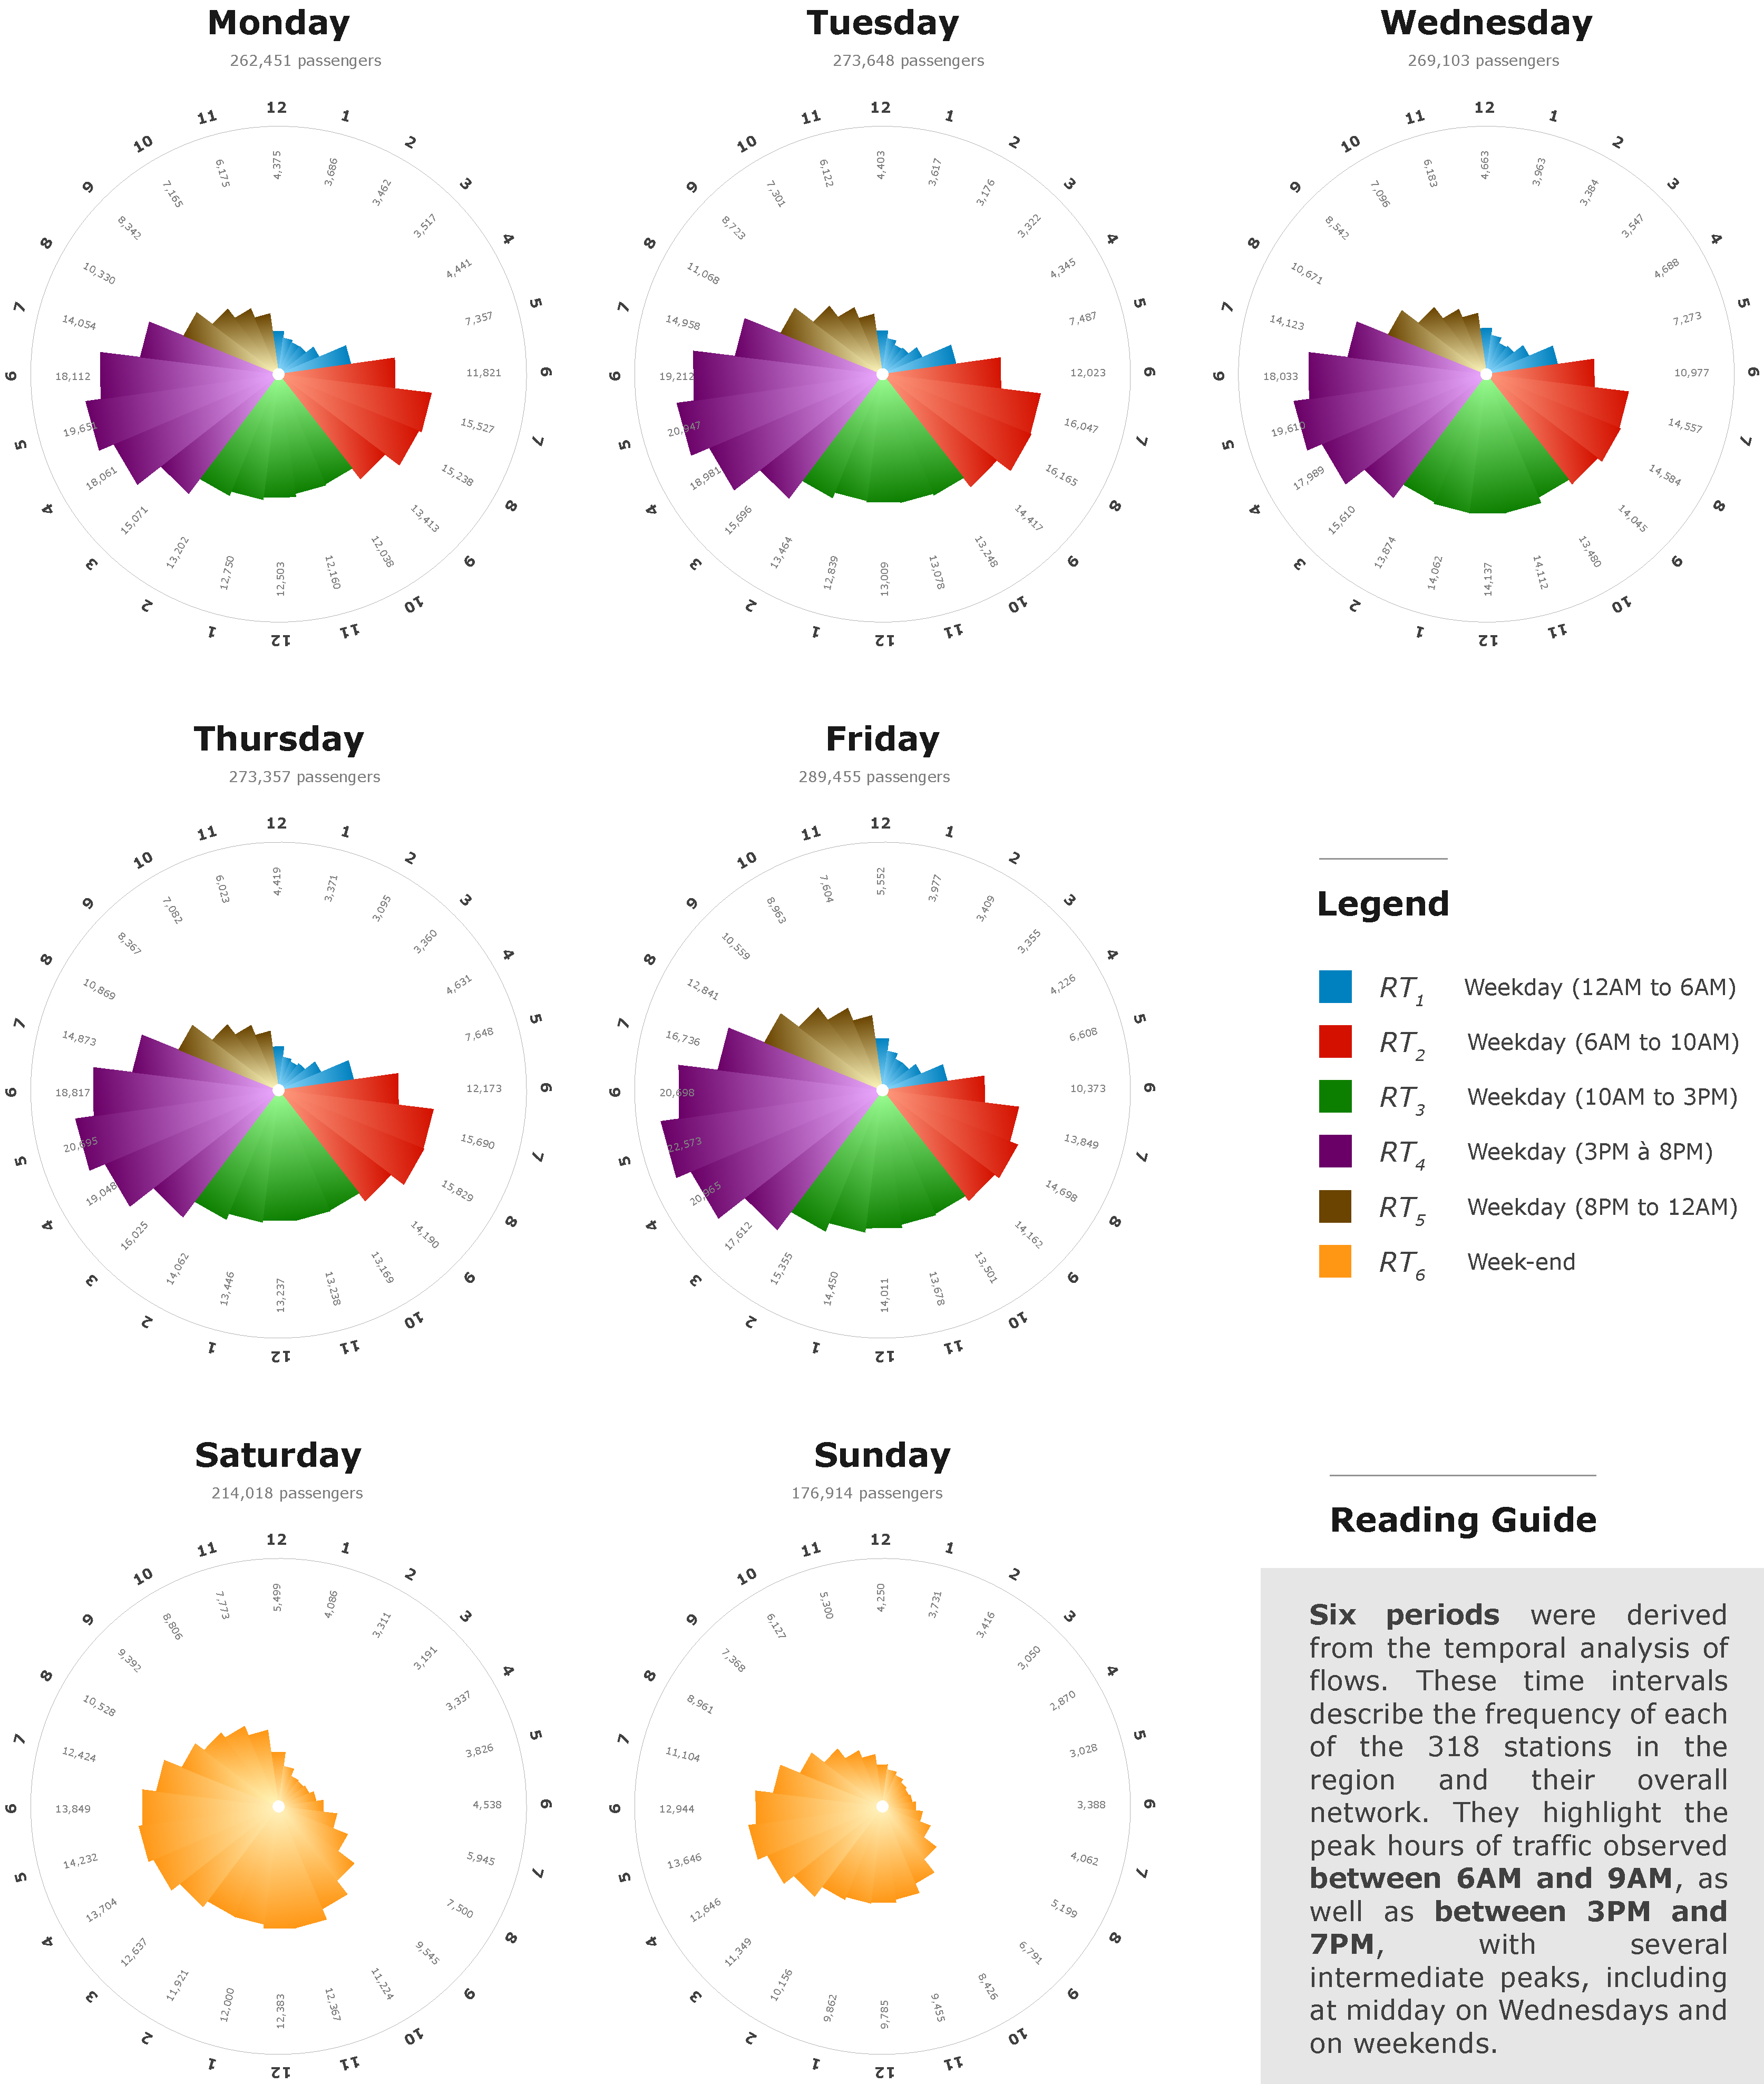
\includegraphics[width=1\columnwidth]{src/Figures/Chap-6/EN_NPART_Flux_frequentation.pdf}}
    \vspace{5pt}
    \begin{flushright}\scriptsize{
    Source: \textcolor{blue}{\textcite{google_maps_google_2024}}\index{Google Maps@\textsl{Google Maps}|pagebf}
    \\
    Realization: \textcolor{blue}{Dylan Moinse (2024)}
    \\
    Authors: \acrshort{NPART} Research Project
    }\end{flushright}
\end{figure}

% Secondary peaks
Wednesday is also distinguished by an intermediate peak between 10:00 AM and 12:00 PM, likely due to the afternoon traditionally given to children, while Friday records a more pronounced ridership maximum during the evening peak period. The identification of an intermediate peak in our observations is supported by the analysis of trip distribution conducted by \textcolor{blue}{Emmanuel} \textcolor{blue}{\textcite[66]{munch_periodes_2017}}\index{Munch, Emmanuel|pagebf} on the SNCF Transilien network for 126 stations in 2015. He refers to these peaks as \Commas{peak shoulders,} located at the transition between peak hours and off-peak hours.
%%Translated%%

    % Périodes
%Cette distribution des flux de passager·ère par période est dès lors inégale: la période \(RT_{4}\) enregistre une proportion nettement supérieure de fréquentation comparée aux autres, tandis que \(RT_{1}\) est bien plus faible en comparaison (voir l'\hyperref[fig-chap6:resultats-frequentation-periode]{illustration~\ref{fig-chap6:resultats-frequentation-periode}}, page~\pageref{fig-chap6:resultats-frequentation-periode}).%%Rédigé%%

% Transition
Although ridership data for the stations is known for a specific week, this information remains both limited and static. In response to this challenge, prediction allows us to move beyond this single observation by anticipating the evolution of usage and external contexts. The value of predicting station flows lies, from a statistical perspective, in the continuous improvement of the model and, from a planning perspective, in optimizing decision-making. With this in mind, we will detail the predictive approach to passenger flow adopted within the \acrshort{NPART} model.
%%Translated%%

% 6.2.4.2.
\needspace{1\baselineskip} % Reserve space
\subsubsection*{Adjustment and Prediction of Ridership at the Studied Stations
    \label{chap6:methodologie-indicateurs-frequentation-prediction}
    }

% Introduction
The prediction of passenger volume primarily aims to anticipate flows in order to highlight the levers of action that could promote a modal shift towards public transport, while enhancing its management. The development of predictive models addresses the need for continuous improvement of these models and better forecasting of fluctuations due to events, seasonal variations, or long-term trends. To this end, through a scientific collaboration between the \acrfull{LVMT} at the University Gustave Eiffel, \acrfull{SUSE}, and \acrfull{SCU}, we applied several statistical techniques from \textsl{Machine Learning}\footnote{~
    Machine learning is a sub-discipline of \acrfull{AI} that allows computer systems to autonomously learn from input data. Such a model is capable of identifying patterns, relationships, and making predictions or decisions based on supervised training data. \textsl{Machine Learning} has various applications, ranging from prediction and classification to speech and image recognition, as well as text analysis.
} by adopting an ensemble learning model\footnote{~
    Ensemble learning involves combining several models, called \Commas{weak learners,} to improve accuracy compared to a single model. This \textsl{Machine Learning} approach enhances overall performance by reducing generalization error, i.e., the difference between performance on training data and new data (i), model variance by smoothing individual predictions (ii), and model biases (iii).
}, after normalizing the collected data:
\begin{customitemize}
    \item \acrfull{MLR}, or multiple linear regression, models the linear relationship between explanatory variables and the target variable, namely the number of railway passengers;
    \item \acrfull{KNN}, or the k-nearest neighbors method, predicts ridership by identifying the \(k\) most similar moments in the past and calculating an average of the corresponding riderships;
    \item \acrfull{ANN}, or neural networks, capture the complex and non-linear relationships between variables, inspired by the architecture of the human brain.
    %\item \acrfull{SVM}, or \textsl{Support Vector Machines}, and logistic regression were used to model relationships between variables when the previous techniques were not suitable.
\end{customitemize}
%%Translated%%

% Ensemble learning
The ensemble learning techniques we employed are ensemble averaging\footnote{~
    In this approach, all models are weighted equally, and the final prediction is calculated as the average of the individual predictions.
}, weighted ensemble averaging\footnote{~
    In this case, models are weighted based on their respective performance on the training set; the more accurate models are assigned a higher weight.
}, and stacking\footnote{~
    Stacking involves using the predictions of base models as inputs for a meta-model (in our case, a ridge regression), which produces the final prediction.
}. The evaluation of these models was performed using metrics based on \acrfull{MSE}\footnote{~
    As described in the \hyperref[section-chap4:cyclabilite-genre]{section examining the links between bikeability and gendered use of light individual mobility~\ref{section-chap4:cyclabilite-genre}} (page~\pageref{section-chap4:cyclabilite-genre}), from \hyperref[chap4:titre]{chapter~\ref{chap4:titre}} (page~\pageref{chap4:titre}), \acrfull{MSE} is a commonly used metric to measure the gap between observed values and predicted values by a \textsl{Machine Learning} model, particularly in regression models. One of the disadvantages of this measure is that it amplifies large errors due to the squaring of differences, making the model more sensitive to outliers.
} and \acrfull{APRE}, or average pointwise relative error\footnote{~
    \acrfull{APRE} quantifies the relative error between observed and predicted values, normalizing it by the actual values. This \gls{metric} is particularly useful for evaluating the accuracy of prediction models when the data exhibits significant variations in magnitude. Unlike \acrshort{MSE}, \acrshort{APRE} is less sensitive to outliers since it takes the scale of actual values into account.
}. In both of these metrics, a low value indicates a high-performing model, capable of predicting actual values accurately while minimizing relative errors.
%%Translated%%

% Figure Ridership prediction
\begin{figure}[h!]\vspace*{4pt}
    \caption{Prediction methods for station ridership during morning peak hours (\(RT_{2}\)).}
    \label{fig-chap6:prediction-frequentation}
    \centerline{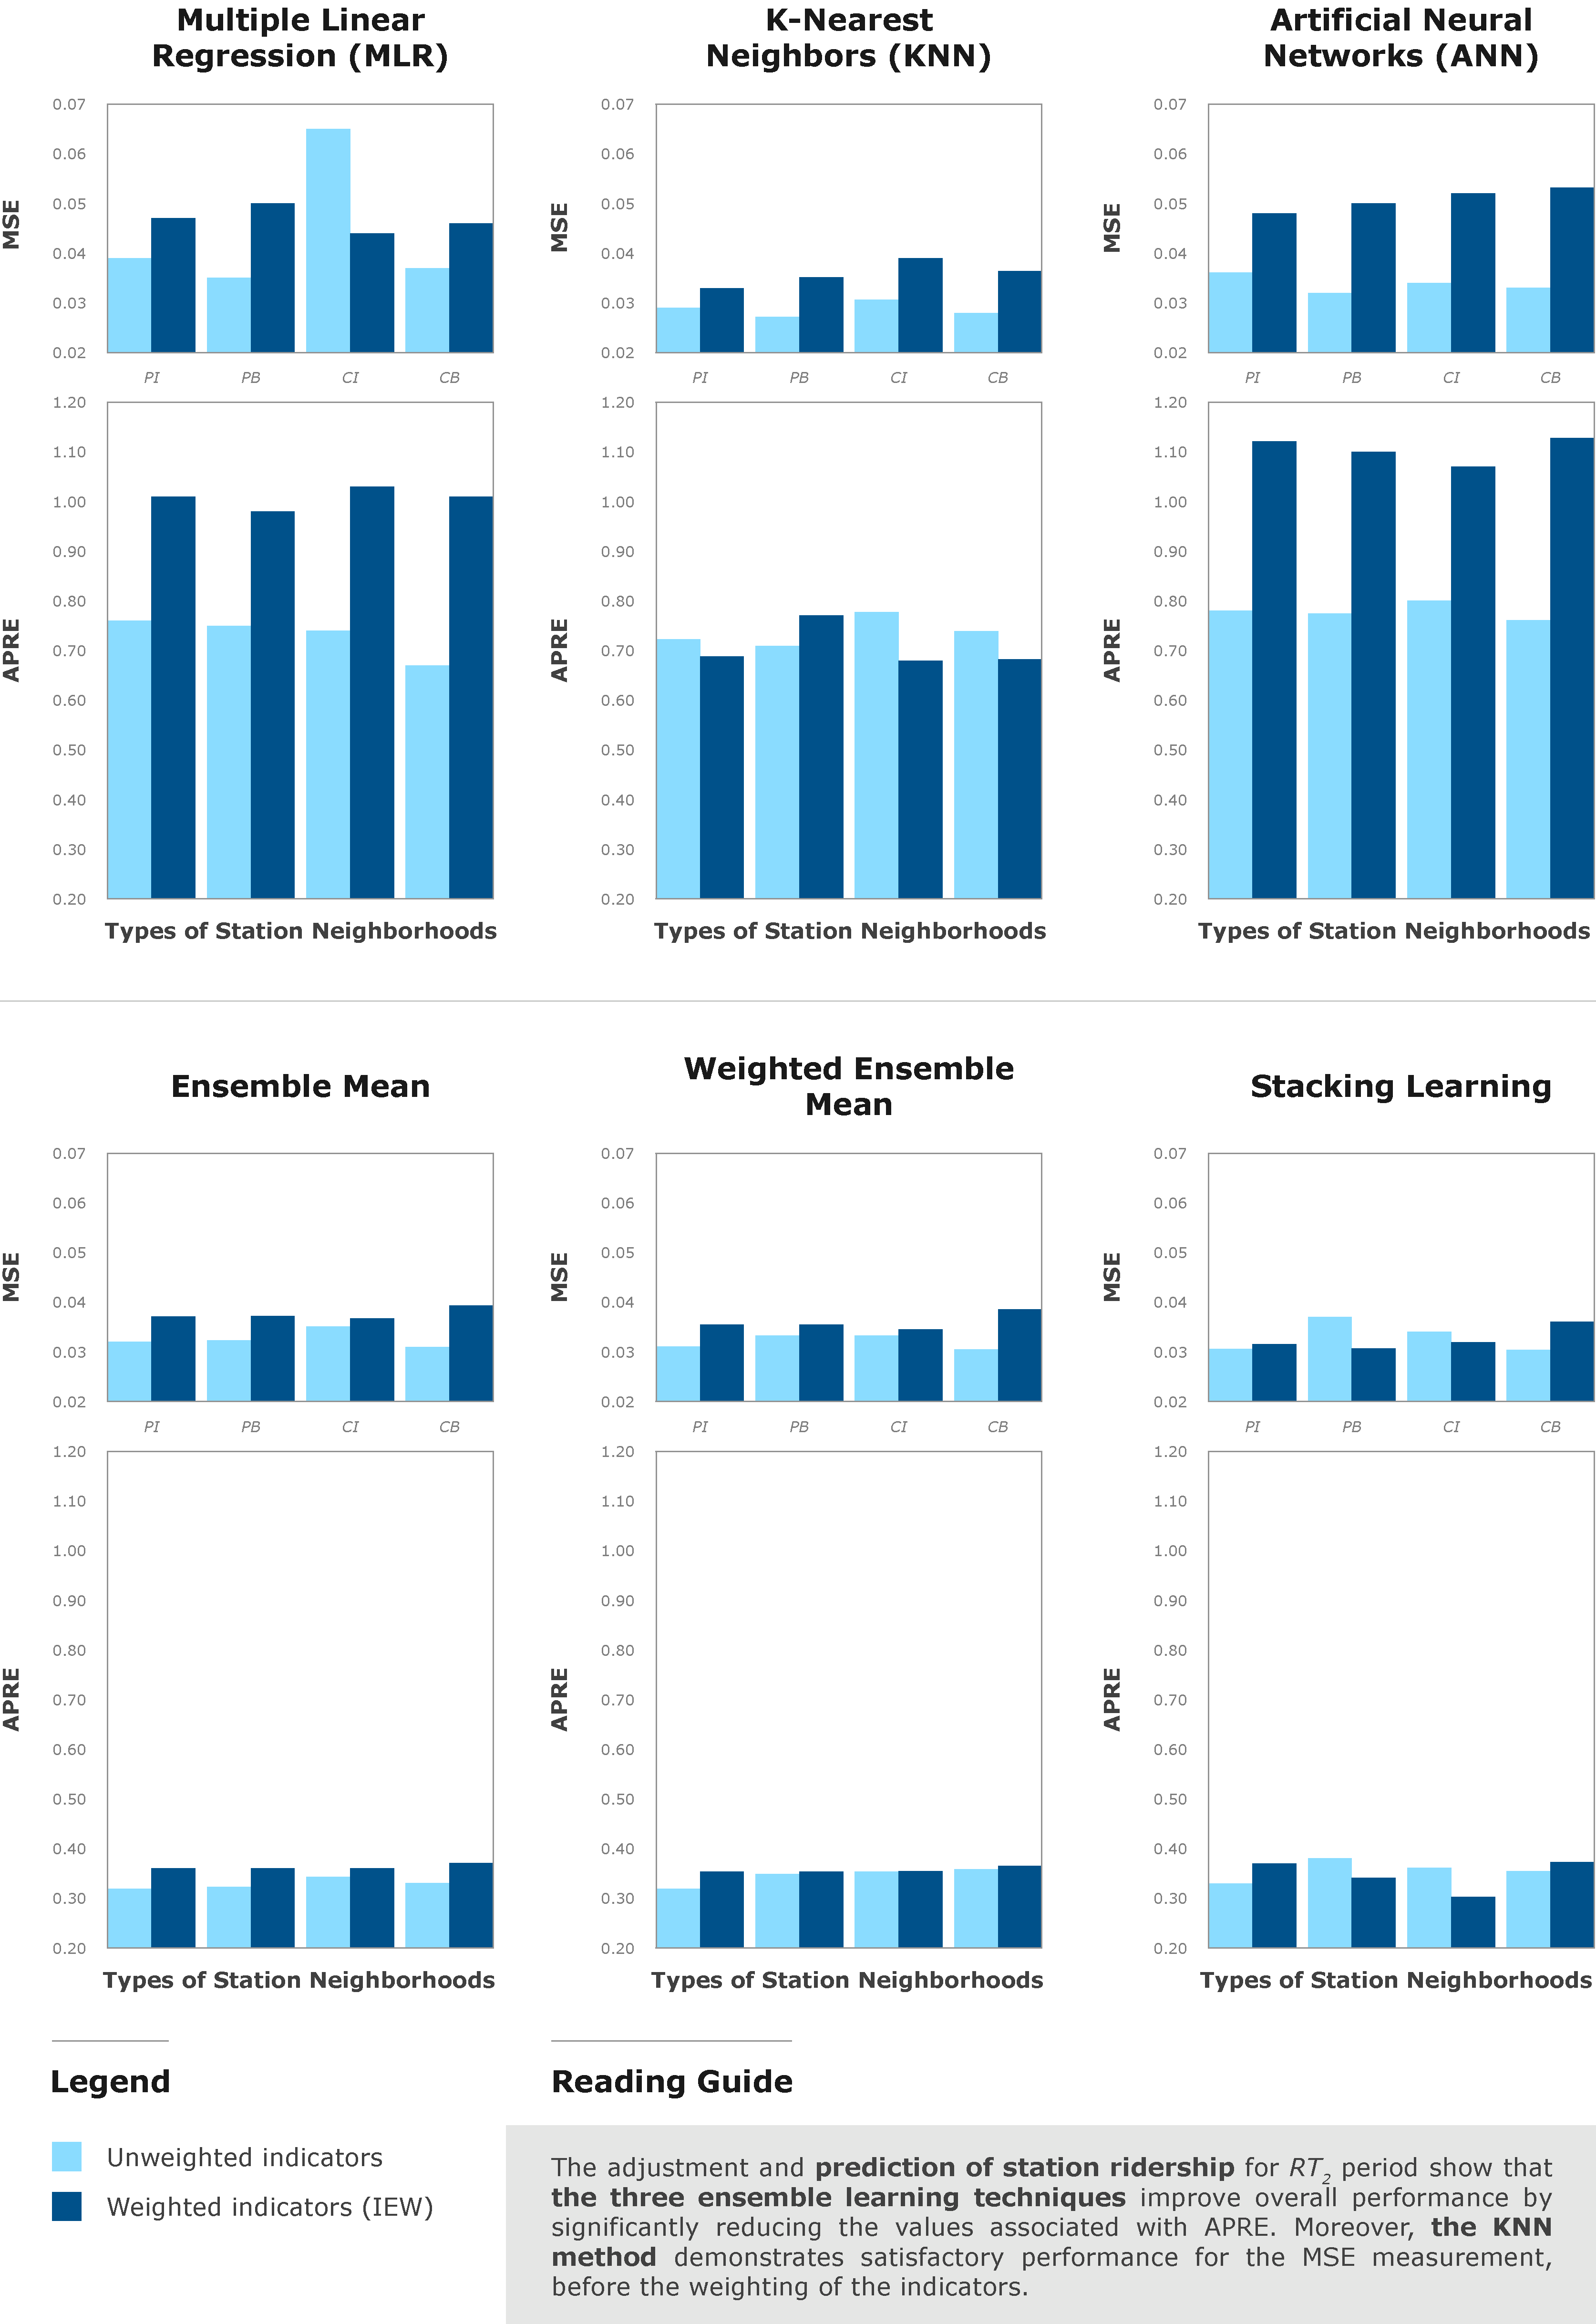
\includegraphics[width=1\columnwidth]{src/Figures/Chap-6/EN_NPART_Prediction_frequentation.pdf}}
    \vspace{5pt}
    \begin{flushright}\scriptsize{
    Realization: \textcolor{blue}{Dylan Moinse (2024)}
    \\
    Authors: \acrshort{NPART} Research Project
    }\end{flushright}
\end{figure}

% Prediction results
The results obtained from these predictive models indicate that all three ensemble learning techniques significantly reduce the \acrshort{APRE}, suggesting an improvement in performance, particularly for low-traffic stations (see \hyperref[fig-chap6:prediction-frequentation]{Figure~\ref{fig-chap6:prediction-frequentation}}, page~\pageref{fig-chap6:prediction-frequentation}). Although the \acrshort{KNN} method shows satisfactory performance before the weighting of explanatory variables, the \acrshort{MLR} and \acrshort{ANN} models exhibit notable improvements after applying this weighting. We compared the evolution of \acrshort{MSE} and \acrshort{APRE} values across different geographical areas and periods. This analysis demonstrated that both \acrshort{KNN} and the three ensemble learning-based predictive models offer a more accurate fit in predicting train station ridership. It follows that these predictive models are particularly beneficial for less crowded stations, for which the accuracy of the forecasts is improved.
%%Translated%%

% Transition questionnaire opinion and relative weight of indicators
Once the indicator grid is defined and the geographical data extraction is completed, the question of their relative weighting arises within the framework of station and train station district classification. While the vast majority of previous \acrshort{NPM} models assign an equal weight to each indicator, a handful of studies highlight the limitations of this calibration method, which may undermine the validity of the classification process. In this context, the following section is dedicated to outlining the different weighting strategies we developed for our modeling.
%%Translated%%

% Transition
After defining the \acrshort{NPART} based on a grid of indicators organized around four key dimensions—the node, the location, accessibility, and ridership—we focus on describing the model calibration steps. The objective of the following section is then to adjust and validate the parameters of the tool used. To this end, we will explore the methods of collecting and analyzing geographical data, and how these techniques ensure better accuracy in the results derived from this model combining network and urban planning.
%%Translated%%

% ___________________________________________
% 6.3.
\newpage
\needspace{1\baselineskip} % Reserve space
\sectionheader{Methods for Collecting and Analyzing Geographical Data}
\section{Data Collection and Analysis Protocol for Modeling the Degree of Coordination Between the Network and Urban Planning at the Scale of the Hauts-de-France Region
    \label{chap6:methodologie-m-tod-index}
    }

% Introduction
The design of our \acrshort{NPART} model is based on the selection of forty quantifiable explanatory indicators and six indicators related to train station ridership. The goal is to classify and qualify the stations and their immediate surroundings within the context of \acrshort{M-TOD} development, for which a methodological protocol has been established. This protocol includes data collection as well as geostatistical analysis. The methodology outlined in this section presents the techniques employed for extraction, normalization, and validation of the measures. This research project is part of an international scientific collaboration involving researchers from the University Gustave Eiffel, \acrfull{SUSE}, and \acrfull{SCU}, with researchers from these two Chinese universities having developed the methodological approach presented here through collaboration and interdisciplinary dialogue with researchers from \acrfull{LVMT}. This methodological process also integrates the classification of stations according to different criteria and the assignment of weights to the indicators, in order to better reflect their relative influence on rail usage. This analysis protocol led to the generation of 288 specific typologies, based on several factors: the analyzed geographical area (\(PI\), \(PB\), \(CI\), and \(CB\)), the studied periods (from \(RT_{1}\) to \(RT_{6}\)), the variable weighting strategies, and the classification procedures applied to the stations (see \hyperref[fig-chap6:schema-methodologie]{Figure~\ref{fig-chap6:schema-methodologie}}, page~\pageref{fig-chap6:schema-methodologie}).
%%Translated%%

% Figure NPART methodology diagram
\begin{figure}[h!]\vspace*{4pt}
    \caption{Flow diagram representing the main methodological steps of the spatial model.}
    \label{fig-chap6:schema-methodologie}
    \centerline{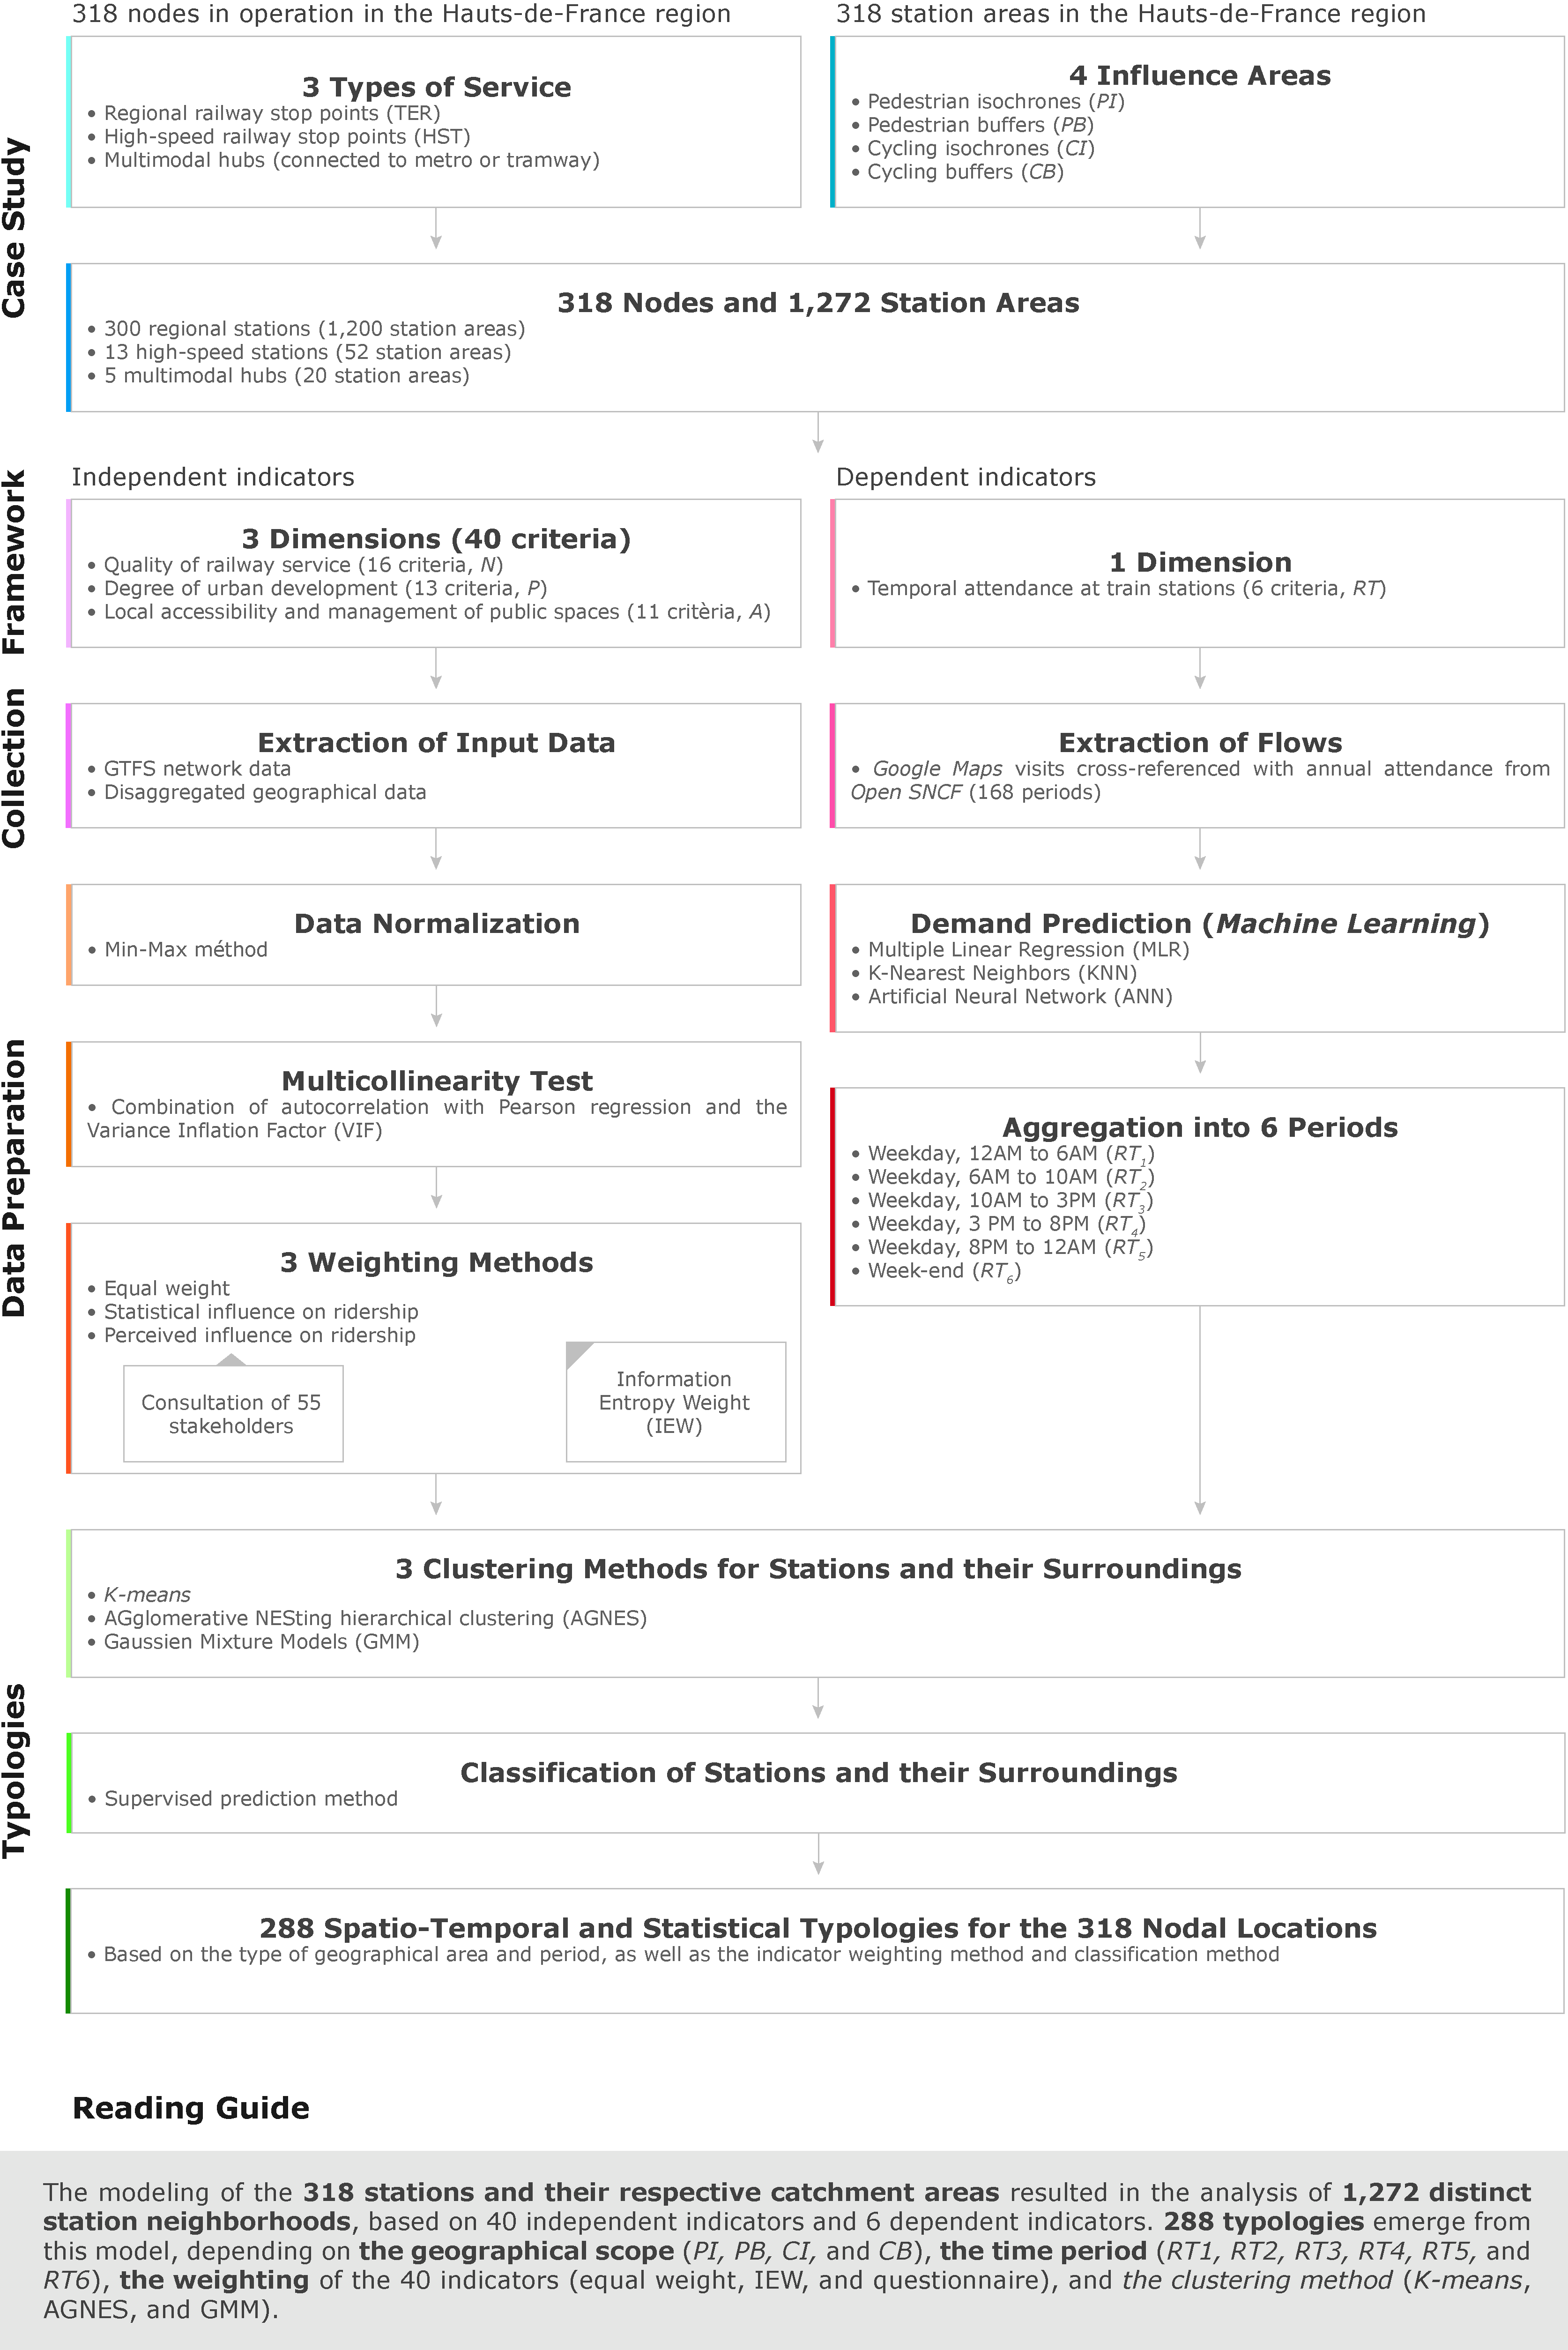
\includegraphics[width=1\columnwidth]{src/Figures/Chap-6/EN_NPART_Schema_Methodologie.pdf}}
    \vspace{5pt}
    \begin{flushright}\scriptsize{
    Realization: \textcolor{blue}{Dylan Moinse (2024)}
    \\
    Authors: \acrshort{NPART} Research Project
    }\end{flushright}
\end{figure}

% Plan outline
As for the outline, we will first present the modeling techniques used to process the collected data, namely the extraction and normalization of statistical and geographical data, their validation through the analysis of the interactions they have with each other, as well as how the stations are classified (see \hyperref[chap6:methodologie-statistiques]{section on extraction, exploitation, and classification processes}, page~\pageref{chap6:methodologie-statistiques}). Next, the focus will be on the attribution of weights to the variables, considering three approaches: equal weight, statistical weighting based on their actual influence on train station ridership, and perceived weighting, established from feedback from planners interviewed (see \hyperref[chap6:methodologie-ponderation-indicateurs]{section on the relative weight of each component}, page~\pageref{chap6:methodologie-ponderation-indicateurs}). Finally, we will discuss the validity, updating, and enhancement of this model through its reproducibility and automation (see \hyperref[chap6:conclusion-valorisation]{section on the requirements for a transparent model capable of being replicated and repeated}, page~\pageref{chap6:conclusion-valorisation}).
%%Translated%%

% 6.3.1.
\needspace{1\baselineskip} % Reserve space
\subsection{Modeling Techniques for Collected Data
    \label{chap6:methodologie-statistiques}
    }

% Introduction
This subsection describes the steps of data collection and analysis related to train stations as well as geographical information, in connection with the buffer zones and isochrones defined. The data preparation preceding the modeling work is primarily based on the search for disaggregated data sources, which are then transformed and scaled to ensure their consistency. Furthermore, the model validation is based on the analysis of interdependencies between the various indicators. Following this statistical analysis, we can adopt a classification approach based on various parameters outlined.%%Translated%%

% 6.3.1.1.
\needspace{1\baselineskip} % Reserve space
\subsubsection*{Extraction and Normalization of Geographical Data
    \label{chap6:methodologie-statistiques-normalisation}
    }

% Geographical Extraction - Train Station Districts
Once the indicator grid was defined in detail, we proceeded with the spatial extraction of the available data. For each interchange point, we selected the defined train station districts, integrating both isochrones and pedestrian buffer zones (\(PB\) and \(PI\)) and cycling zones (\(CB\) and \(CI\)), as outlined in the \hyperref[chap3:quartiers-gare-analyse-geostatistique]{section dedicated to the geographical representation of the train station districts in the region} (page~\pageref{chap3:quartiers-gare-analyse-geostatistique}), in \hyperref[chap3:titre]{Chapter~3} (page~\pageref{chap3:titre}). We deliberately limited ourselves to using disaggregated geographical data in order to maximize the accuracy of the location of the determined variables, except for the values related to the node, which rely solely on \acrshort{GTFS} data provided by institutions and mobility managers. Furthermore, this spatial granularity requirement led to the adoption of estimation methods for data when grouped within spatial grids, such as gridded or hexagonal data, as detailed in the \hyperref[chap3:quartiers-gare-analyse-geostatistique]{section dedicated to the geographical representation of the train station districts in the region} (page~\pageref{chap3:quartiers-gare-analyse-geostatistique}), in \hyperref[chap3:titre]{Chapter~3} (page~\pageref{chap3:titre}).%%Translated%%

% Python VS GIS
In this regard, we chose to use the \textsl{Python} programming language exclusively, particularly its various libraries dedicated to geospatial processing\footnote{~
    \textsl{Python} has a vast ecosystem of libraries for manipulating and visualizing spatial data, the main ones being: \textsl{GeoPandas}, \textsl{Shapely}, \textsl{Pyproj}, \textsl{Fiona}, \textsl{Rtree}, \textsl{GDAL}, \textsl{PySAL}, \textsl{Geopy}, \textsl{OSMNx}, \textsl{NetworkX}, \textsl{H3-Py}, \textsl{Folium}, \textsl{Basemap}, \textsl{Plotly}, \textsl{Geoplot}.
}, in order to extract and analyze the data. This choice is explained by several comparative advantages over the traditional use of \acrfull{GIS}. First, \textsl{Python} offers greater flexibility in data processing, being both more adaptable and easily customizable. Additionally, it allows for the manipulation of large datasets and the automation of data extraction and transformation processes through the various scripts generated. Furthermore, \textsl{Python} facilitates complex calculations, thereby enabling the extraction of the required data, especially when they require combinations of diverse datasets. Finally, the analysis of \acrshort{GTFS} data is greatly simplified, particularly by enabling the modeling of complex networks and graph analysis.%%Translated%%

% Normalization of Collected Data
The normalization of input data is a critical step before any modeling, \textsl{a fortiori} within the framework of \acrshort{NPM}. In this context, the data collected for each train station must be homogenized to prevent scale differences between variables from disproportionately influencing the model's results. To achieve this, the Min-Max normalization method\footnote{~
    Since nodal characteristics such as location, accessibility, or ridership can be expressed in different units, normalization standardizes these values so that they can be integrated coherently into the \acrshort{NPART}, without one indicator or dimension dominating the others. In this regard, the Min-Max method preserves the relative distribution of the data while maintaining the relationships between values. This standardization of variables ensures the use of analysis techniques that are sensitive to data scale, such as regressions or distance-based algorithms (k-means), which will be applied later.
} was applied prior to the training phase. This technique consists of transforming the values of each variable to ensure they fall between 0 and 1 (see \hyperref[equation:normalisation]{Formula~\ref{equation:normalisation}}, page~\pageref{equation:normalisation}).%%Translated%%

% Normalization Equation
\begin{equation}
\label{equation:normalisation}
\begin{aligned}
x_i' = \frac{x_i - \min(x_i)}{\max(x_i) - \min(x_i)}
\end{aligned}
\end{equation}
\begin{align*}
    &\text{where:}\\
    &x \text{ is the original value;}\\
    &x' \text{ is the normalized value;}\\
    \min(x) \text{ and } \max(x) & \text{ are the minimum and maximum values.}\\
\end{align*}%%Translated%%

% Transition
After data collection and normalization, it is important to ensure that the transformed variables are ready to be integrated into the model. A key preparatory step before modeling is to check for multicollinearity\footnote{~
    Multicollinearity is a statistical situation in which several explanatory variables in a model are highly correlated with each other. In other words, the independent variables exhibit redundancy, which can pose problems for interpreting results in regression models, such as multiple linear regression. When multicollinearity is present, the coefficients of the independent indicators may become unstable, reducing the accuracy of predictions and statistical significance. The variance inflation factor (\(VIF\)), greater than 100, as well as correlation coefficients close to 1 or -1, generally indicate strong multicollinearity between the variables.
} of the data, that is, the existence of excessive correlations between certain variables. The presence of multicollinearity can compromise the interpretation of the model's results and harm its accuracy, particularly in analyses based on relationships between variables. Therefore, before entering the actual modeling phase, an analysis of multicollinearity is essential to validate the consistency of the data and ensure their relative independence.%%Translated%%

% 6.3.1.2.
\needspace{1\baselineskip} % Reserve space
\subsubsection*{Validation of Collected Geographical Data through Interaction Analysis
    \label{chap6:methodologie-statistiques-validation}
    }

% Multicollinearity
We assessed multicollinearity between the independent variables using two statistical approaches: the simple correlation coefficient, using Pearson's correlation coefficient \(R^{2}\), and the variance inflation factor (\(VIF\)). By combining these two methods, we can identify and remove independent variables exhibiting very high collinearity problems. \hyperref[fig-chap6:correlations-indicateurs-independants-PI]{Figures~\ref{fig-chap6:correlations-indicateurs-independants-PI}} and \hyperref[fig-chap6:correlations-indicateurs-independants-CI]{\ref{fig-chap6:correlations-indicateurs-independants-CI}} (pages \pageref{fig-chap6:correlations-indicateurs-independants-PI} and \pageref{fig-chap6:correlations-indicateurs-independants-CI}) illustrate the interrelationships between the explanatory criteria.%%Translated%%

% Figure regressions independent indicators PI
\begin{figure}[h!]\vspace*{4pt}
    \caption{Correlation matrix of the spatial model, at the scale of pedestrian isochrones.}
    \label{fig-chap6:correlations-indicateurs-independants-PI}
    \centerline{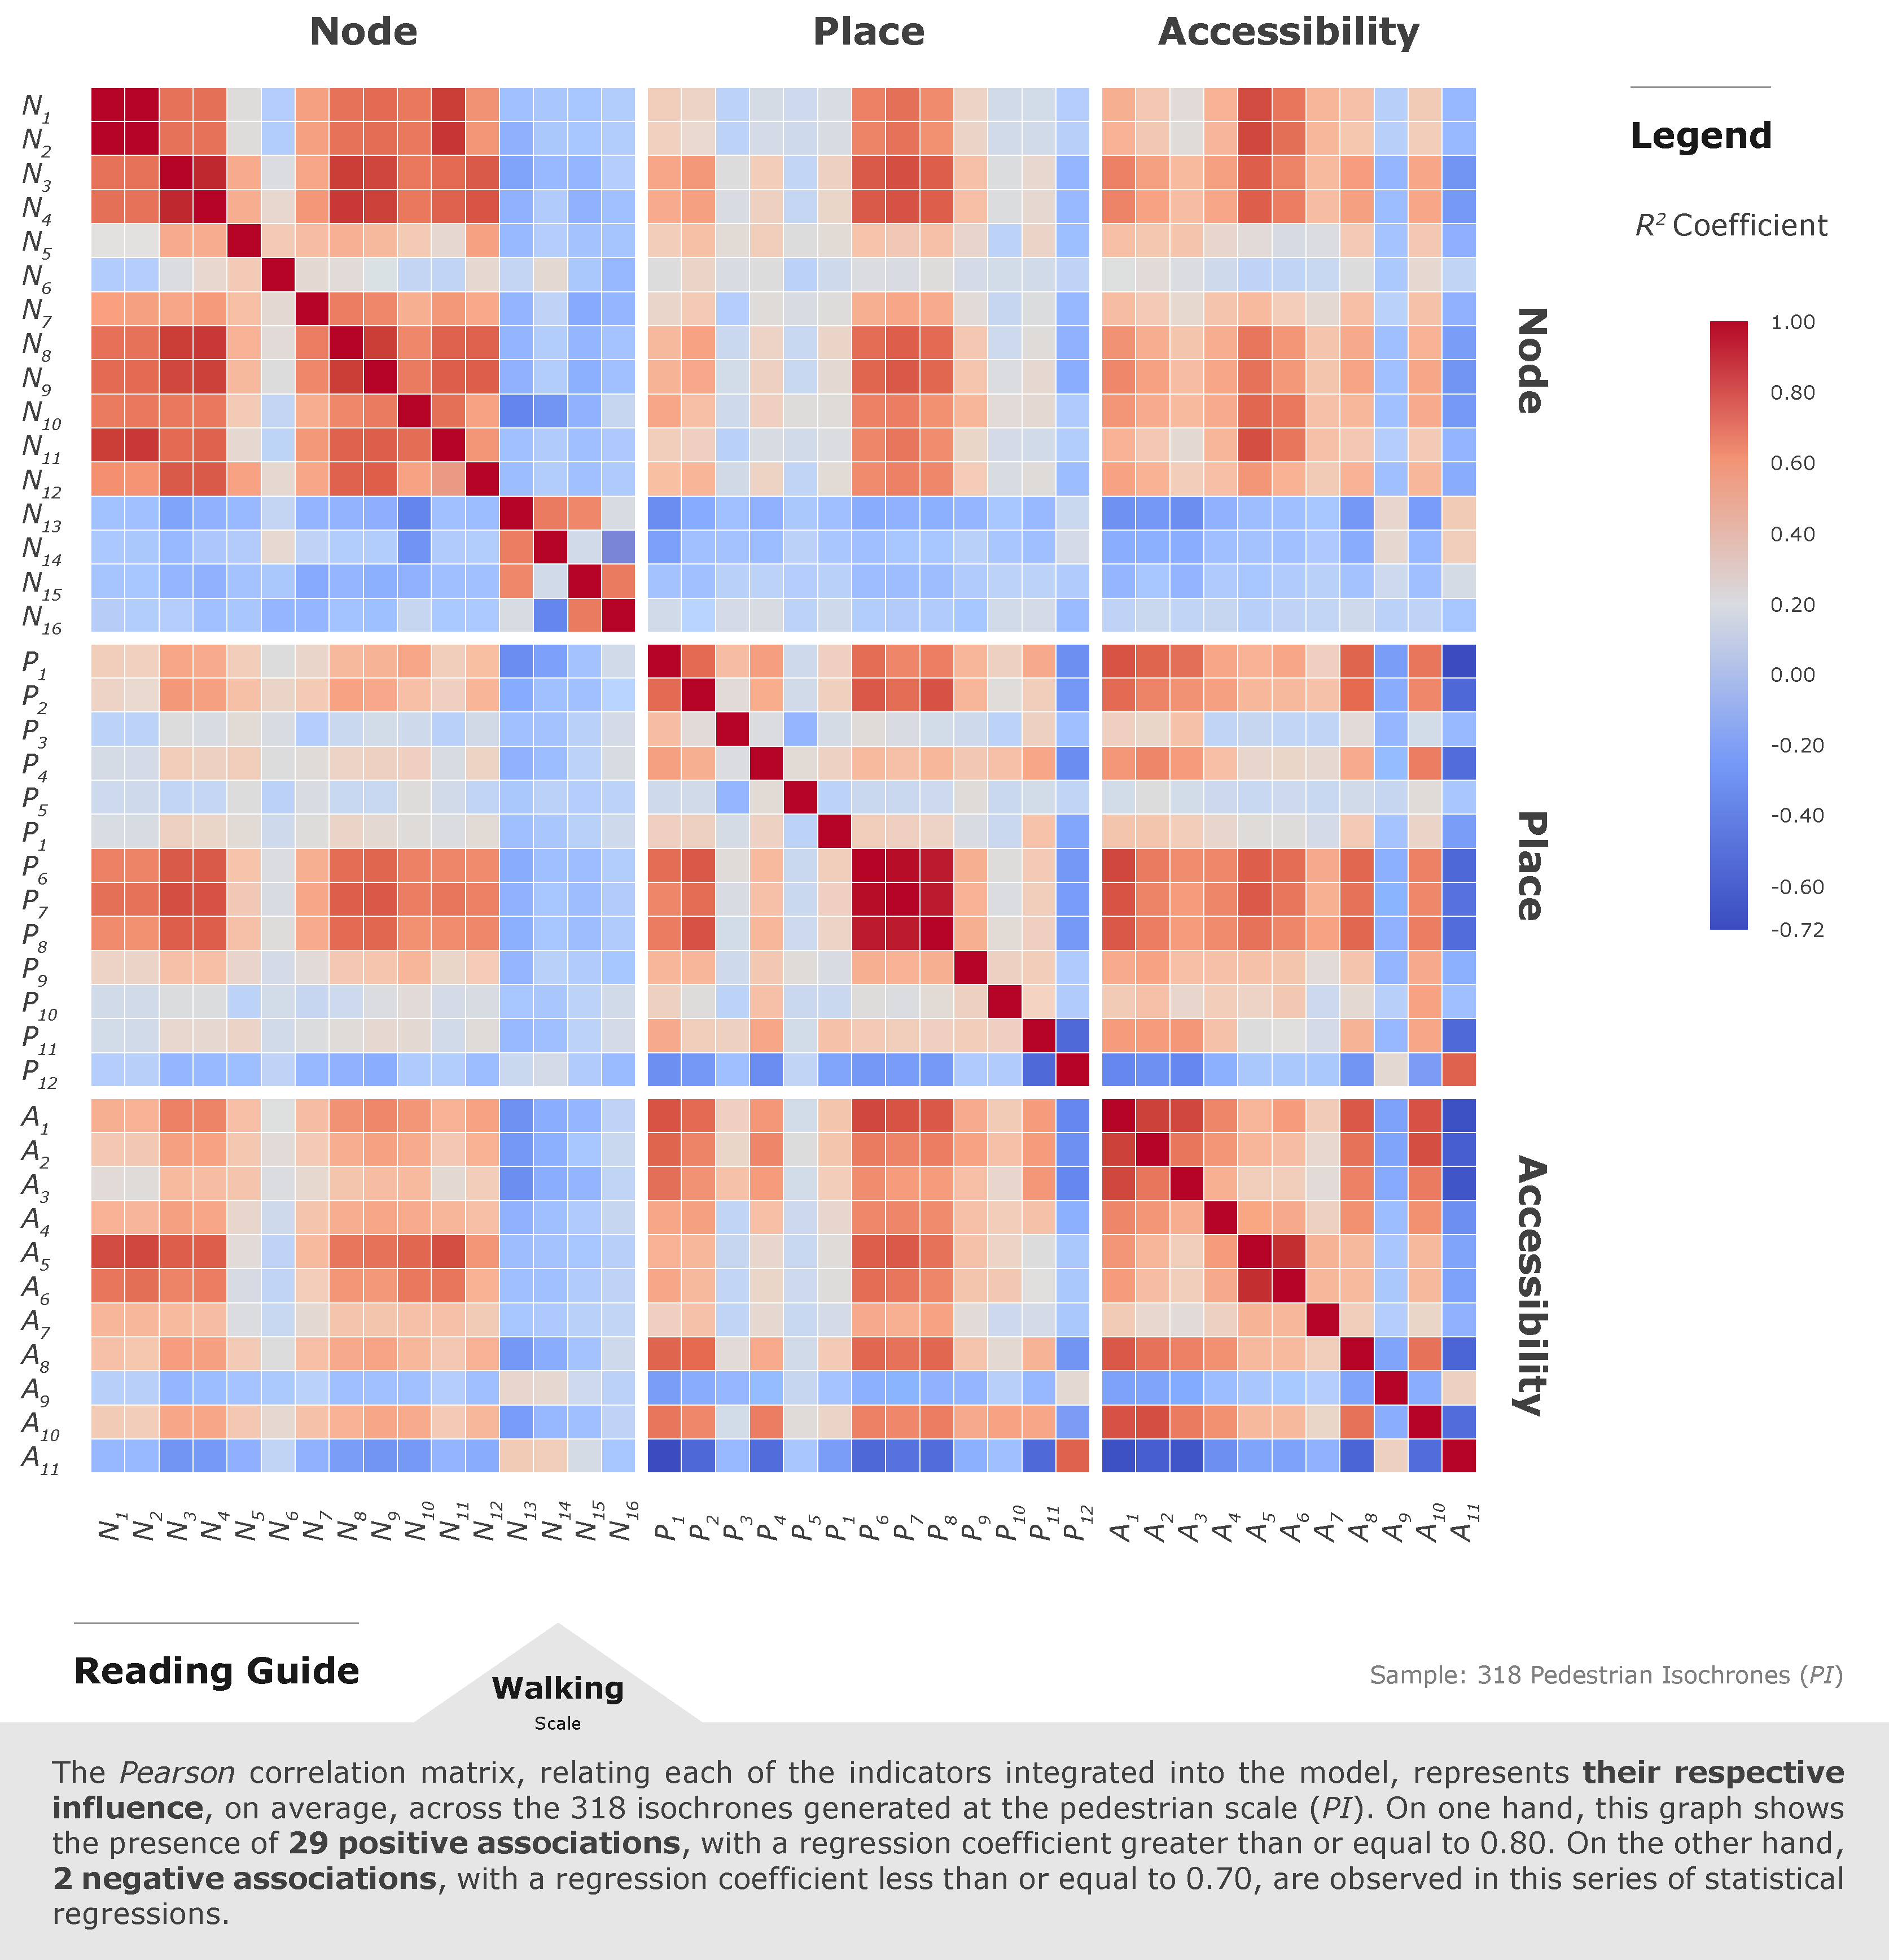
\includegraphics[width=1\columnwidth]{src/Figures/Chap-6/EN_NPART_Matrice_Correlation_PI.pdf}}
    \vspace{5pt}
    \begin{flushright}\scriptsize{
    Realization: \textcolor{blue}{Dylan Moinse (2024)}
    \\
    Authors: \acrshort{NPART} Research Project
    }\end{flushright}
\end{figure}

% Figure regressions independent indicators CI
\begin{figure}[h!]\vspace*{4pt}
    \caption{Correlation matrix of the spatial model, at the scale of cycling isochrones.}
    \label{fig-chap6:correlations-indicateurs-independants-CI}
    \centerline{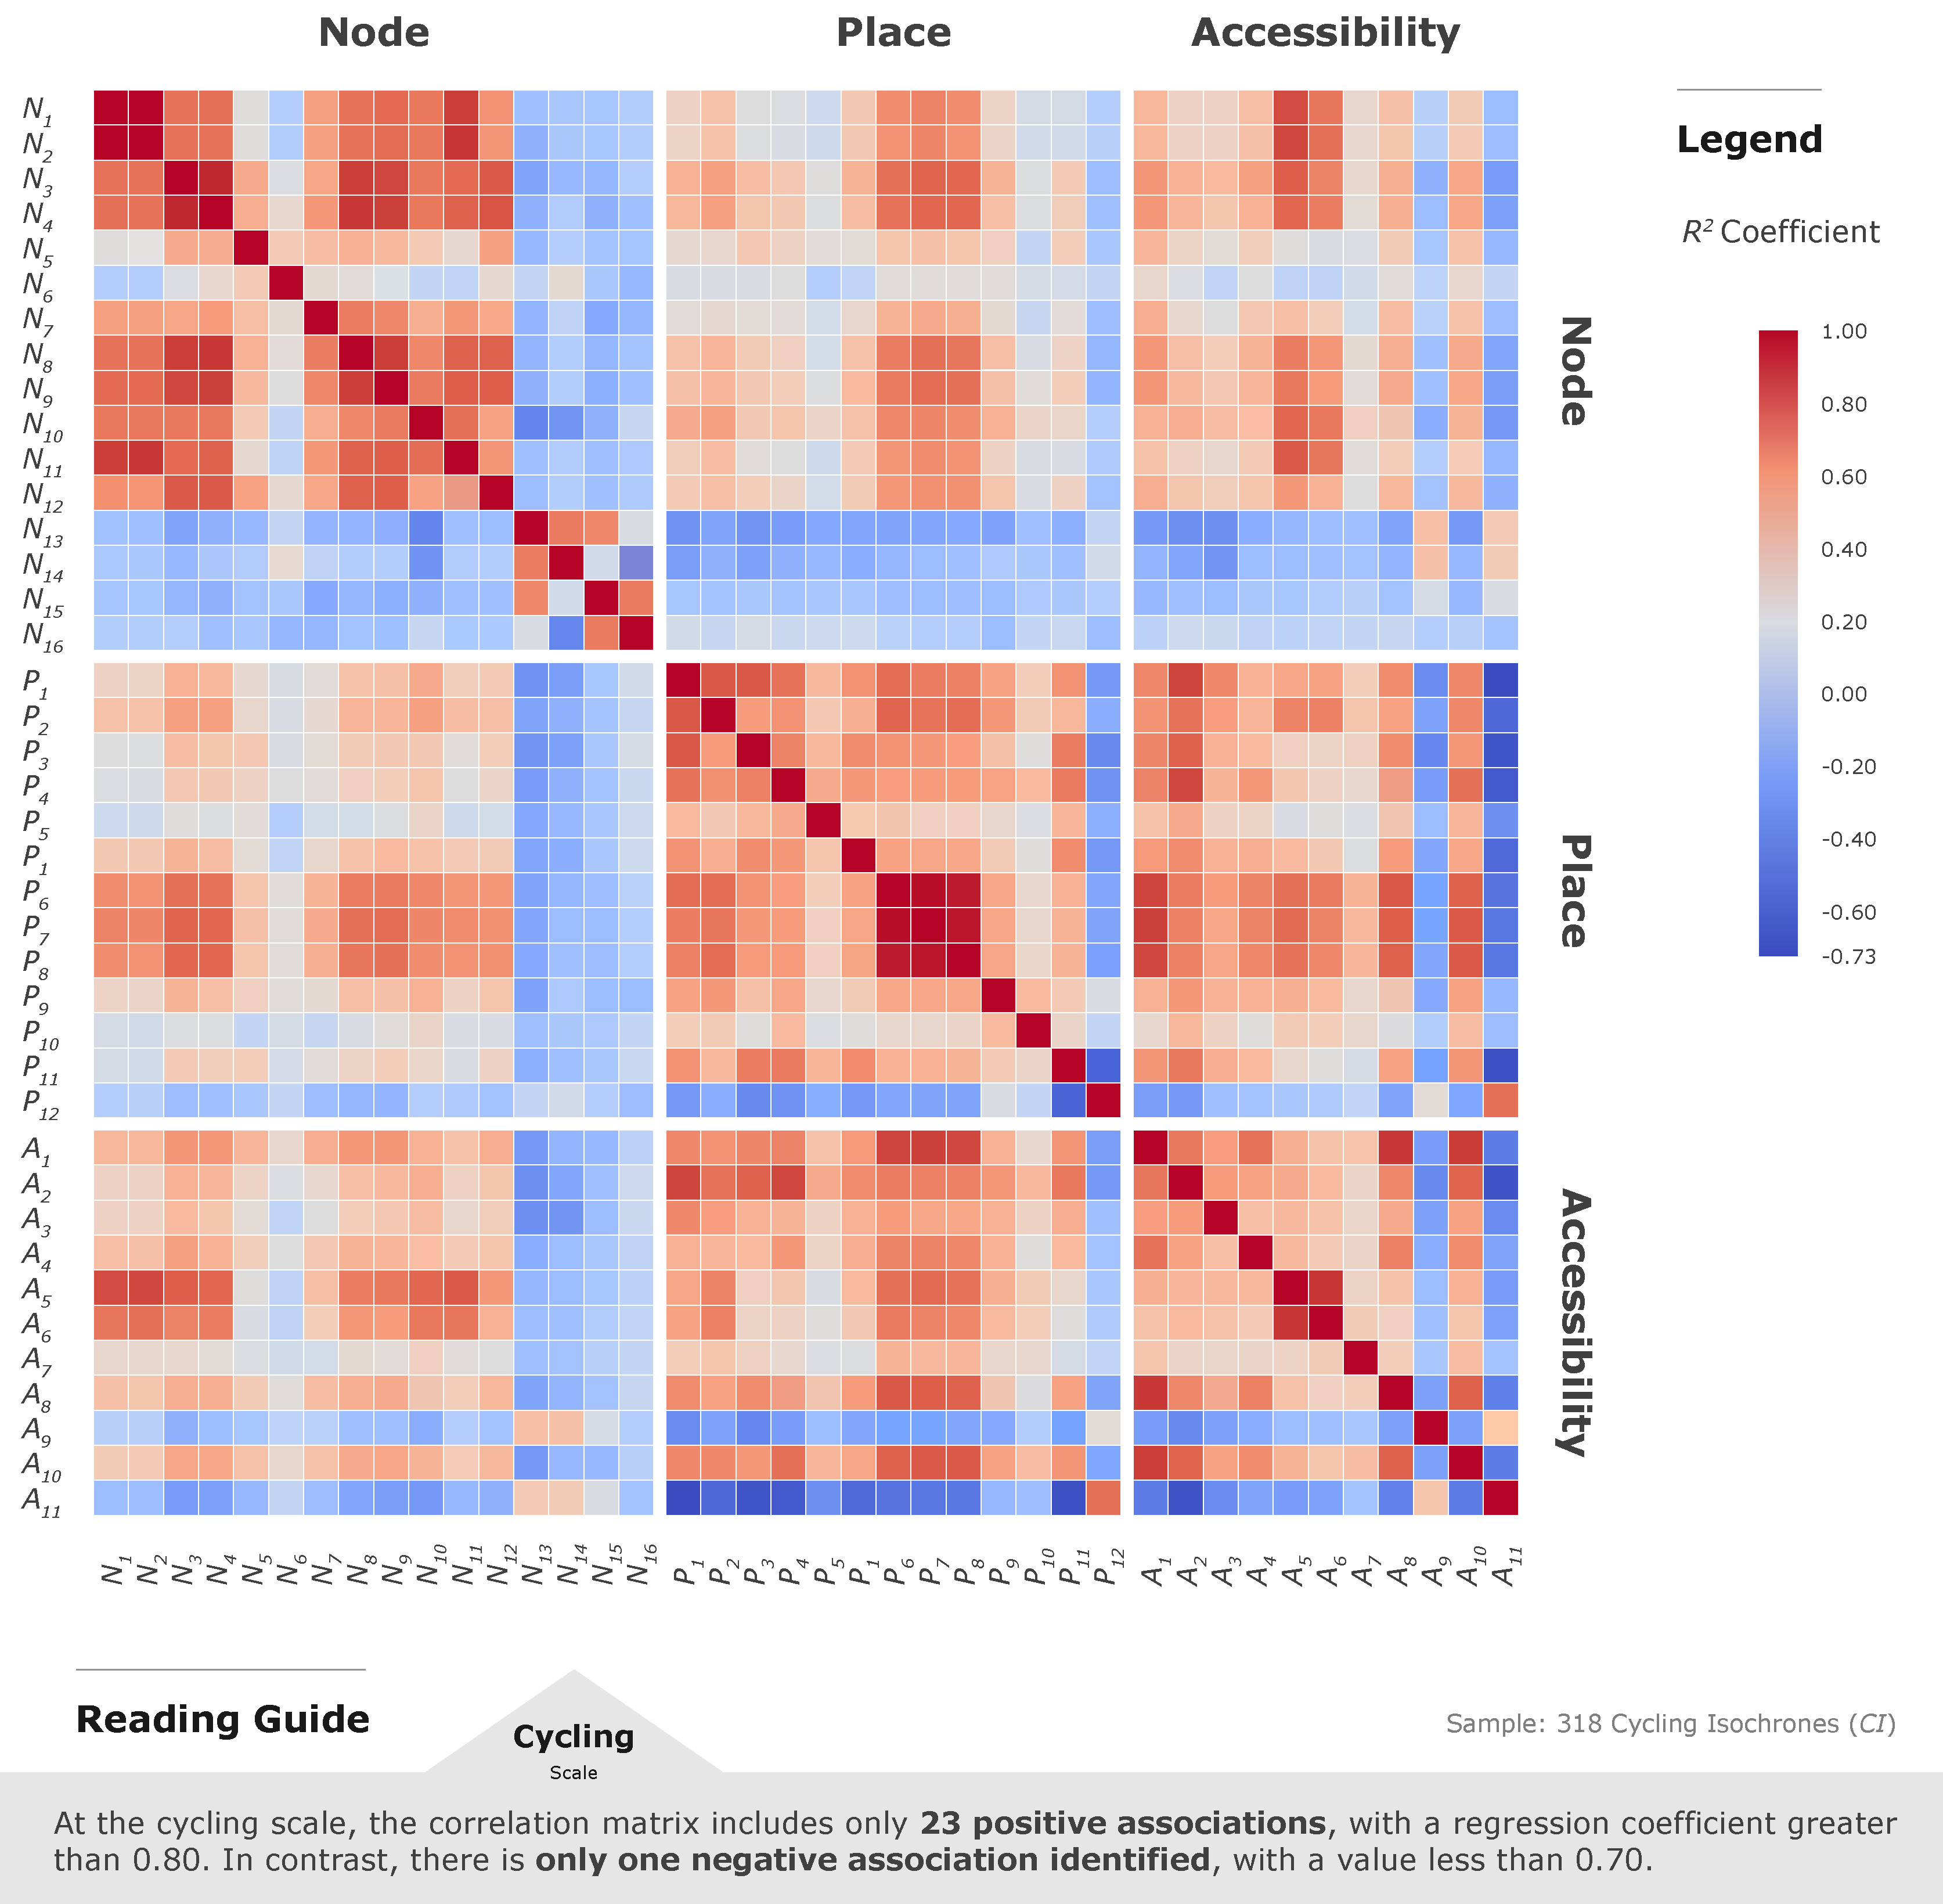
\includegraphics[width=1\columnwidth]{src/Figures/Chap-6/EN_NPART_Matrice_Correlation_CI.pdf}}
    \vspace{5pt}
    \begin{flushright}\scriptsize{
    Realization: \textcolor{blue}{Dylan Moinse (2024)}
    \\
    Authors: \acrshort{NPART} Research Project
    }\end{flushright}
\end{figure}

% Correlation Results: Within the Node
Within the dimension related to the level of service at the station, the regression suggests that the frequency of the \acrshort{TER} network (\(N_{3}\) and \(N_{4}\)) shows a significant positive association, not only with the number of directions served (\(N_{8}\), \(R^{2}\) at 0.89 and 0.90), but also with the degree of centrality (\(N_{9}\), \(R^{2}\) at 0.86 and 0.88) and with the number of stations accessible within an hour (\(N_{12}\), \(R^{2}\) at 0.80). As for the frequency of the \acrshort{HST} network (\(N_{1}\) and \(N_{2}\)), it is correlated with the proximity centrality (\(N_{11}\), \(R^{2}\) at 0.89 and 0.90). Moreover, the aforementioned indicators \(N_{8}\) and \(N_{9}\) show a positive association (\(R^{2}\) at 0.89).%%Translated%%

% Correlation Results: Pedestrians and Cyclists Within the Place
Regarding the level of urban development, several positive associations between indicators are observed, both at the pedestrian (\(PI\)) and cycling (\(CI\)) scales. Population density (\(P_{1}\)) is correlated with employment density (\(P_{2}\), \(R^{2}_{PI}\) at 0.75 and \(R^{2}_{CI}\) at 0.81), and with proximity \acrshort{POIs} (\(P_{7}\), \(R^{2}_{PI}\) and \(R^{2}_{CI}\) at 0.74). The three types of \acrshort{POIs} are also correlated with employment density (\(P_{7}\), \(P_{8}\), and \(P_{9}\), \(R^{2}_{PI}\) and \(R^{2}_{CI}\) between 0.71 and 0.83), and with each other (\(R^{2}_{PI}\) and \(R^{2}_{CI}\) between 0.96 and 0.98). As expected, the average household income (\(P_{13}\)) is negatively correlated with the proportion of social housing (\(P_{12}\), \(R^{2}_{PI}\) at -0.60 and \(R^{2}_{CI}\) at -0.62). However, several positive associations are exclusively visible within the cycling train station districts, notably between \(P_{1}\) and land use predominantly residential (\(P_{3}\), \(R^{2}_{CI}\) at 0.81), predominantly commercial (\(P_{4}\), \(R^{2}_{CI}\) at 0.72), and with \(P_{7}\) (\(R^{2}_{CI}\) at 0.74).%%Translated%%

% Results correlation between pedestrians and cyclists: within accessibility
Finally, the regression examining the indicators related to the dimension of public space management reveals various positive associations. The length of the pedestrian network (\(A_{1}\)) is positively associated with intersection density (\(A_{2}\), \(R^{2}_{PI}\) at 0.88 and \(R^{2}_{CI}\) at 0.71), bus service (\(A_{8}\), \(R^{2}_{PI}\) at 0.81 and \(R^{2}_{CI}\) at 0.90), car parking (\(A_{10}\), \(R^{2}_{PI}\) at 0.83 and \(R^{2}_{CI}\) at 0.89), and spatial efficiency at the pedestrian scale (\(A_{3}\), \(R^{2}_{PI}\) at 0.86 and \(R^{2}_{CI}\) at 0.55). Intersection density is correlated with spatial efficiency (\(R^{2}_{PI}\) at 0.71 and \(R^{2}_{CI}\) at 0.56), the presence of bus stops (\(R^{2}_{PI}\) at 0.72 and \(R^{2}_{CI}\) at 0.64), and the area of car parking (\(R^{2}_{PI}\) at 0.84 and \(R^{2}_{CI}\) at 0.77). While the latter indicator is positively associated with the bus network (\(R^{2}_{PI}\) at 0.72 and \(R^{2}_{CI}\) at 0.78). Bicycle parking is correlated with the fleet of \acrshort{PBS} (\(R^{2}_{PI}\) at 0.93 and \(R^{2}_{CI}\) at 0.91). The household motorization rate is negatively associated with a multitude of variables, including the pedestrian network (\(R^{2}_{PI}\) at -0.70 and \(R^{2}_{CI}\) at -0.53), intersection density (\(R^{2}_{PI}\) at -0.65 and \(R^{2}_{CI}\) at -0.69), spatial efficiency (\(R^{2}_{PI}\) at -0.68 and \(R^{2}_{CI}\) at -0.46), and bus stops (\(R^{2}_{PI}\) at -0.62 and \(R^{2}_{CI}\) at -0.51). Finally, railway station neighborhoods for cyclists have a specific positive association, between the pedestrian network and the cycling network (\(R^{2}_{CI}\) at 0.72).%%Translated%%

    % Résultats corrélation piétons et cyclables : entre les dimensions
%Capacité de stationnement vélo avec la fréquence des lignes \acrshort{TGV} (\(R^{2}_{PI}\) à 0,86 et \(R^{2}_{CI}\) à 0,85) et la centralité de proximité (\(R^{2}_{PI}\) à 0,83 et \(R^{2}_{CI}\) à 0,80). Fréquence des lignes \acrshort{TER} avec les \acrshort{POIs} de tous types (\(R^{2}_{PI}\) et \(R^{2}_{CI}\) entre 0,72 et 0,84). Réseau piéton et densité de population (\(R^{2}_{PI}\) à 0,82 et \(R^{2}_{CI}\) à 0,64), les \acrshort{POIs} de tous types (\(R^{2}_{PI}\) et \(R^{2}_{CI}\) entre 0,81 et 0,88), et inversement avec le taux de motorisation (\(R^{2}_{PI}\) et \(R^{2}_{CI}\) à -0,72), tout comme avec la proportion de logements sociaux (\(R^{2}_{PI}\) à -0,60 et \(R^{2}_{CI}\) à -0,70), avec les \acrshort{POIs} de \Commas{proximité} (\(R^{2}_{PI}\) à -0,61 et \(R^{2}_{CI}\) à -0,56), avec la densité de population (\(R^{2}_{PI}\) et \(R^{2}_{CI}\) à -0,72) et avec la densité d'emploi (\(R^{2}_{PI}\) à -0,61 et \(R^{2}_{CI}\) à -0,61).

% Removal of criteria
As a general rule, we consider that an independent variable poses a significant collinearity problem when \(R^{2}\) reaches 0.90 or when \(VIF\) exceeds 100.00. Therefore, the variables we might consider excluding are the frequency of the \acrshort{HST} networks (\(N_{2}\)), intermediary centrality (\(N_{10}\)), proximity \acrshort{POIs} (\(P_{7}\)), and the household motorization rate (\(A_{11}\)) for all train station neighborhood configurations (\(PB\), \(PI\), \(CB\), and \(CI\)). The method used to adjust this model is \acrfull{OLS}, or Ordinary Least Squares regression. This technique aims to determine the optimal regression line by minimizing the sum of squared deviations between the observed and predicted values. The \acrfull{MSE} is used to assess the accuracy of the model's predictions, thus measuring its overall performance.%%Translated%%

% Choice of criteria conservation
After eliminating the indicators \(N_{2}\), \(N_{10}\), \(P_{7}\), and \(A_{11}\) for each geographical and temporal scope considered, the parameters of the different regression models show that the adjustment effect has barely changed. As a result, we decided to retain all the initially defined indicators because, from a geographical perspective, they more accurately reflect the complexity of urban reality. In this regard, we draw on the conclusions of \textcolor{blue}{\textcite[16]{cao_coordination_2020}}\index{Cao, Zhejing|pagebf}\index{Asakura, Yasuo|pagebf}\index{Tan, Zongbo|pagebf}, which demonstrate that the \acrshort{NPM} model, after eliminating variables with a too high \(VIF\), is ultimately less precise than the full model retaining all the indicators.%%Translated%%

% Transition
After performing the analysis of multicollinearity among the variables, it is now possible to proceed with the clustering and classification of the train stations. Proper management of multicollinearity is a crucial prerequisite to ensure a reliable and interpretable typology, leading to homogeneous and representative groups.%%Translated%%

% 6.3.2.
\needspace{1\baselineskip} % Reserve space
\subsection{Double Exploratory and Predictive Approach through Partitioning and Classification
    \label{chap6:methodologie-statistiques-clusterisation-classification}
    }

% Interest of classification
Classification\footnote{~
    From a statistical perspective, classification is a supervised learning technique in which the model is trained on a labeled dataset. Unlike clustering, which is an unsupervised learning method aimed at grouping similar observations without prior knowledge of the labels. The goal of clustering is to discover structures within the data by organizing them into clusters. Thus, classification seeks to learn to predict the labels of new data, while clustering focuses on identifying inherent structures within the data, grouping them based on similarity or distance measures.
}, as an analytical framework, aims to group train stations into different homogeneous sets based on similar characteristics, to better guide urban planning decisions \textcolor{blue}{\autocite[2]{cao_coordination_2020}}\index{Cao, Zhejing|pagebf}\index{Asakura, Yasuo|pagebf}\index{Tan, Zongbo|pagebf}. The main goal of this approach is to organize a dataset into clusters\footnote{~
    A cluster is defined as a group of train stations sharing common attributes, identified by clustering algorithms according to a distance or similarity measure in a multidimensional space \textcolor{blue}{\autocite[7]{everitt_cluster_2011}}\index{Everitt, Brian~S.|pagebf}\index{Landau, Sabine|pagebf}\index{Leese, Morven|pagebf}\index{Stahl, Daniel|pagebf}. According to \textcolor{blue}{R.~M.} \textcolor{blue}{\textcite[321]{cormack_review_1971}}\index{Cormack,~R.~M.|pagebf} and \textcolor{blue}{A.~D.} \textcolor{blue}{\textcite[15]{gordon_classification_1999}}\index{Gordon,~A.~D.|pagebf}, a cluster is characterized by its internal cohesion, expressed in terms of \textsl{homogeneity}, and its external isolation, defined by the \textsl{separation} between groups. Indeed, a classification algorithm will theoretically aim to ensure lower intra-class variability, i.e., minimizing the distance between individuals within the same group, and higher inter-class variability, i.e., maximizing the distance between individuals from different groups.
}, in order to facilitate understanding and concisely summarize the similarities and differences present in the data. The value of a classification often lies in its practical usefulness rather than its absolute truth \textcolor{blue}{\autocite[4]{everitt_cluster_2011}}\index{Everitt, Brian~S.|pagebf}\index{Landau, Sabine|pagebf}\index{Leese, Morven|pagebf}\index{Stahl, Daniel|pagebf}. For \textcolor{blue}{A.~D.} \textcolor{blue}{\textcite[5]{gordon_classification_1999}}\index{Gordon,~A.~D.|pagebf}. Such an approach allows synthesizing complex databases and helps in detecting structures and interactions within this information. If distinct classes of objects are identified, they can then be named, their properties defined, and consequently, it facilitates the assignment of new objects. In this sense, the concept of \Commas{similarity} linked to classification techniques is both central and subjective, as the definition of clustering algorithms and the interpretation of results are subject to the judgment of the modelers.%%Translated%%

% Two-step approach
Our approach consists of two steps: clustering followed by classification. First, clustering is used to segment the initially unlabeled train stations into meaningful groups based on their characteristics. Then, classification involves assigning each train station a label corresponding to its cluster and using these labels to train a supervised model capable of predicting the cluster of a train station based on its characteristics. The resulting supervised model not only allows for predicting the cluster when new stations are integrated but also helps identify the most influential variables for classification. The value of this combined approach lies in adopting an exploratory approach to understand and segment the data, followed by a predictive approach to generalize the results and make predictions on new data.%%Translated%%

% 6.3.2.1.
\needspace{1\baselineskip} % Reserve space
\subsubsection*{Data Grouping Exercise
    \label{chap6:methodologie-statistiques-clusterisation}
    }

% Clustering
The first step consisted of clustering the train stations using three different methods:
\begin{customitemize}
    \item The first method is the k-means method\footnote{~
        The goal of the k-means method is to minimize the errors represented by the \acrfull{WCSS}, or the sum of squared intra-cluster distances, defined as the sum of squared Euclidean distances between data samples and the corresponding centroid in the original algorithm \textcolor{blue}{\autocite[4]{barve_reef-insight_2023}}\index{Barve, Saharsh|pagebf}\index{Webster, Jody~M.|pagebf}\index{Chandra, Rohitash|pagebf}. Each observation is assigned to the cluster whose mean, i.e., the cluster center, is the closest. The algorithm proceeds in four steps: initialization by randomly selecting \(k\) initial centers (i), (re)assigning each object to the cluster whose center minimizes the distance (ii), updating the centroid by taking the mean of the assigned observations (iii), and convergence through successive iterations until a maximum number is reached (iv).
    } \textcolor{blue}{\autocite[281]{macqueen_methods_1967}}\index{MacQueen,~J.~B.|pagebf}, undoubtedly one of the most commonly used methods, even dominant, among \acrshort{NPM} models \textcolor{blue}{\autocites[132]{caset_planning_2019}[12]{cao_coordination_2020}[248]{yang_tod_2021}[5]{liao_evaluating_2022}[3]{amini_pishro_integrated_2023}[628]{wei_classifying_2023}[2]{zhou_introducing_2023}}\index{Liao, Cong|pagebf}\index{Scheuer, Bronte|pagebf}\index{Amini Pishro, Ahad|pagebf}\index{L'Hostis, Alain|pagebf}\index{Chen, Dong|pagebf}\index{Chen, Mojdeh|pagebf}\index{Amini Pishro, Mojdeh|pagebf}\index{Zhang, Zhengrui|pagebf}\index{Li, Jun|pagebf}\index{Zhao, Yuandi|pagebf}\index{Zhang, Lili|pagebf}\index{Shen, Zhongwei|pagebf}\index{Xie, Yi|pagebf}\index{Liang, Pengpeng|pagebf}\index{Yu, Bingjie|pagebf}\index{Chen, Li|pagebf}\index{Cao, Zhejing|pagebf}\index{Asakura, Yasuo|pagebf}\index{Tan, Zongbo|pagebf}\index{Wei, Sheng|pagebf}\index{Wang, Lei|pagebf}\index{Caset, Freke|pagebf}\index{Yang, Liu|pagebf}\index{Song, Xiaoyu|pagebf}\index{Zhou, Mingzhi|pagebf}\index{Zhou, Jiali|pagebf}\index{Zhou, Jiangping|pagebf}\index{Lei, Shuyu|pagebf}\index{Zhao, Zhan|pagebf}. It is particularly effective for partitioning data into a predefined number of clusters characterized by similarities. This unsupervised clustering technique has the advantage of being relatively scalable when processing large datasets but requires specifying the number \(k\) of clusters in advance;
    \item The second technique is \acrfull{AGNES}, or agglomerative hierarchical clustering\footnote{~
        \acrfull{AGNES} operates on four principles \textcolor{blue}{\autocite[5]{barve_reef-insight_2023}}\index{Barve, Saharsh|pagebf}\index{Webster, Jody~M.|pagebf}\index{Chandra, Rohitash|pagebf}: each observation is considered as an individual cluster (i), the two most similar clusters are merged at each step (ii), and this merging process continues until a global cluster is formed (iii) represented by a hierarchical tree (iv).
    } that constructs a so-called \textsl{bottom-up} hierarchy of nested clusters, represented in the form of a dendrogram, unlike the k-means partitioning method \textcolor{blue}{\autocite[199]{kaufman_finding_1990}}\index{Kaufman, Leonard|pagebf}\index{Rousseeuw, Peter~J.|pagebf}. This approach allows for identifying groupings of train stations at different levels of granularity, thus revealing subgroups within larger clusters. It determines an appropriate number of clusters based on observed breaks in the hierarchy, implicitly containing all \(k\) values\footnote{~
        There are two main clustering approaches \textcolor{blue}{\autocite[2]{struyf_clustering_1997}}\index{Struyf, Anja|pagebf}\index{Huber, Mia|pagebf}\index{Rousseeuw, Peter~J.|pagebf}. On the one hand, partitioning methods, such as k-means, divide the data into \(k\) distinct clusters, requiring the number of clusters to be specified in advance. On the other hand, hierarchical methods, illustrated by the \acrshort{AGNES} algorithm, build a hierarchy of nested clusters without the need to specify \(k\) beforehand.
    }. This method is particularly effective at capturing subtle nuances and similarities in small to medium-sized data \textcolor{blue}{\autocite[5]{barve_reef-insight_2023}}\index{Barve, Saharsh|pagebf}\index{Webster, Jody~M.|pagebf}\index{Chandra, Rohitash|pagebf}. To our knowledge, only the \textsl{NPM} model developed by \textcolor{blue}{\textcite[3]{olaru_place_2019}}\index{Olaru, Doina|pagebf}\index{Moncrieff, Simon|pagebf}\index{McCarney, Gary|pagebf}\index{Sun, Yuchao|pagebf}\index{Reed, Tristan|pagebf}\index{Pattison, Cate|pagebf}\index{Smith, Brett|pagebf}\index{Biermann, Sharon|pagebf} has employed this hierarchical clustering method;
    \item The last clustering technique used is the \acrfull{GMM} method, also known as Gaussian Mixture Models\footnote{~
        The \acrshort{GMM} model relies on three parameters: the mean which defines the center of each Gaussian distribution (i), the covariance which represents the spread of the distribution (ii), and the mixing probability which indicates the relative weight of the Gaussian distributions (iii) \textcolor{blue}{\autocite[5]{barve_reef-insight_2023}}\index{Barve, Saharsh|pagebf}\index{Webster, Jody~M.|pagebf}\index{Chandra, Rohitash|pagebf}.
    }, a probabilistic model assuming that data are generated from a combination of several normal distributions with unknown parameters. This algorithm assigns \Commas{fuzzy} memberships to the clusters, meaning that each data point has a probability of belonging to each cluster\footnote{~
        The k-means method uses strict assignment, where each point is exclusively assigned to a single cluster. In contrast, the \acrshort{GMM} method operates with fuzzy assignment, giving each point a probability of belonging to each cluster.
    }, which is particularly useful when clusters overlap. Unlike k-means, which assumes spherical and homogeneous clusters, this probabilistic method allows for ellipsoidal clusters with different variances and orientations. However, this approach can be computationally expensive for large datasets. To date, only the publication by \textcolor{blue}{\textcite[5]{caset_integrating_2020}}\index{Caset, Freke|pagebf}\index{Blainey, Simon|pagebf}\index{Derudder, Ben|pagebf}\index{Boussauw, Kobe|pagebf}\index{Witlox, Frank|pagebf} has applied this method for the development of an \acrshort{NPM} model.
\end{customitemize}%%Translated%%

% 6.3.2.2.
\needspace{1\baselineskip} % Reserve space
\subsubsection*{On the \textsl{Optimal} Number of Clusters
    \label{chap6:methodologie-statistiques-nombre-clusters}
    }

% Number of k 1
To determine the optimal number of clusters \(k\), we chose to use the silhouette coefficient (\(SC\)) and the Calinski-Harabasz index, also known as the variance criterion (\(CH\) \textsl{Index}). These two measures are commonly used to assess the quality of data groupings in the three considered unsupervised algorithms (k-means, \acrshort{AGNES}, and \acrshort{GMM}). The silhouette coefficient quantifies the similarity of objects within the same cluster while evaluating their distinction from objects in other clusters. It allows for analyzing the internal cohesion and separation of clusters, providing a fine evaluation at the data point level, with values ranging from -1 to 1. As for the variance criterion, it measures the ratio of inter-cluster variance to intra-cluster variance, with unbounded values. This criterion is particularly useful for comparing different numbers of clusters and various clustering models, relying on the overall dispersion of points. For all these indices, a high value indicates better performance.%%Translated%%

% Number of k 2
The goal of these indices is to identify the point at which adding new clusters no longer significantly improves their values \textcolor{blue}{\autocite[23]{jahaniana_selecting_2022}}\index{Jahaniana, Mojtaba|pagebf}\index{Karimi, Abbas|pagebf}\index{Zarafshan, Faraneh|pagebf}. This point indicates that the clustering model is balanced and that the number of clusters is reasonably chosen. By identifying the optimal \(k\) threshold, it is thus possible to avoid an excess of clusters while ensuring a coherent segmentation of the stations and their surroundings. According to our measurements, the optimal number of \(k\) is set to three for all three clustering methods. As an example, when \(k = 3\) and the parameters are set to \(RT_{2}\), it appears that the k-means algorithm yields the best scores in terms of cluster separation, both for \(PI\) and \(CI\) (see \hyperref[table-chap6:valeurs-indices-sc-ch-ari-jc]{Table~\ref{table-chap6:valeurs-indices-sc-ch-ari-jc}}, page~\pageref{table-chap6:valeurs-indices-sc-ch-ari-jc}).%%Translated%%

% 6.3.2.3.
\needspace{1\baselineskip} % Reserve space
\subsubsection*{Classification of Segmentations
    \label{chap6:methodologie-statistiques-classification}
    }

% Classification
Subsequently, the classification of train stations, which follows a clustering step, involves assigning new observations to pre-existing clusters. This phase relies on the use of a supervised prediction method, where the objective is to predict the membership of each new train station to one of the clusters defined during the initial clustering phase \textcolor{blue}{\autocite[134-135]{james_introduction_2013}}\index{James, Gareth|pagebf}\index{Witten, Daniela|pagebf}\index{Hastie, Trevor|pagebf}\index{Tibshirani, Robert|pagebf}. This approach also allows for the integration of new data on an ongoing basis and keeps the classification updated without requiring a complete re-modeling. Thus, it aims to automate the process of categorizing train stations, based on the clusters identified during the exploratory analysis.%%Translated%%

    % Tableau indices SC / CH / ARI / JC
% Table SC / CH / ARI / JC Indices
%%Translated%%
    \begin{table}[h!]
    \centering
    \renewcommand{\arraystretch}{1.5}
    \resizebox{\columnwidth}{!}{
    \begin{tabular}{p{0.47\columnwidth}p{0.23\columnwidth}p{0.18\columnwidth}p{0.12\columnwidth}}
        %\hline
    \rule{0pt}{15pt} \small{\textbf{\textcolor{blue}{Indices}}} & \small{\textbf{\textcolor{blue}{k-means}}} & \small{\textbf{\textcolor{blue}{\acrshort{AGNES}}}} & \small{\textbf{\textcolor{blue}{\acrshort{GMM}}}} \\
        \hline
    \multicolumn{4}{l}{\textcolor{blue}{\textbf{Walking Isochrones} (\(PI\))}}\\
\small{Silhouette coefficient (\(SC\))} & \small{0.41} & \small{0.48} & \small{0.15}\\
\small{Calinski-Harabasz index (\(CH\))} & \small{248.78} & \small{231.21} & \small{57.51}\\
\small{Adjusted Rand Index (\(ARI\))} & \small{0.36} & \small{0.43} & \small{0.16}\\
\small{Jaccard coefficient (\(JC\))} & \small{0.44} & \small{0.67} & \small{0.49}\\
        \hdashline
    \multicolumn{4}{l}{\textcolor{blue}{\textbf{Cycling Isochrones} (\(CI\))}}\\
\small{Silhouette coefficient (\(SC\))} & \small{0.47} & \small{0.42} & \small{0.16}\\
\small{Calinski-Harabasz index (\(CH\))} & \small{257.31} & \small{204.44} & \small{64.62}\\
\small{Adjusted Rand Index (\(ARI\))} & \small{0.65} & \small{0.74} & \small{0.28}\\
\small{Jaccard coefficient (\(JC\))} & \small{0.74} & \small{0.77} & \small{0.54}\\
        \hline
        \end{tabular}}
    \caption{Review of overall clustering method performance.}
    \label{table-chap6:valeurs-indices-sc-ch-ari-jc}
        \vspace{5pt}
        \begin{flushleft}\scriptsize{
        \textcolor{blue}{Note:} The presented values depend on the case where \(k = 3\) with the time segment \(RT_{2}\).
        \\
        \textcolor{blue}{Reading Guide:} Clustering method performance varies according to the indices and isochrones, with cycling isochrones generally showing better results, particularly for the silhouette index and the adjusted Rand index in the k-means method.
        }\end{flushleft}
        \begin{flushright}\scriptsize{
        Realization: \textcolor{blue}{Dylan Moinse (2024)}
        \\
        Authors: \acrshort{NPART} Research Project
        }\end{flushright}
        \end{table}%%Rédigé%%

% Classification method
To achieve this, we used neural networks. The training of the neural networks was based on consistently labeled points. As shown by the previous results, different clustering methods yield varied outcomes. However, we consider that points consistently classified by the three algorithms legitimately belong to these clusters. In contrast, for points labeled inconsistently, it is not possible to directly and explicitly classify them into these clusters. This is why we decided to perform a second clustering on these inconsistent data. For this, we used the consistently labeled data to train the neural network, hoping that it would have a better ability to classify the unclassified points. We allocated 80\% of this data for model training, and the remaining 20\% served as a validation set to test the model's performance. Once the predictions were made by the neural network, each train station was assigned to a cluster. This cluster is considered to result from the combination of the outcomes of the three clustering algorithms, with the model being trained on data that was classified with a reasonable degree of accuracy. Therefore, we consider this classification result to be sufficiently accurate to be compared with the outcomes of the clustering algorithms, thus allowing for a reassessment of their effectiveness.%%Translated%%

% Verification
To validate the clustering and classification processes, we employed the Adjusted Rand Index (\(ARI\)) and the Jaccard Coefficient (\(JC\)). These two measures are used to assess the similarity between two partitions in order to evaluate the quality of a clustering in comparison to a reference classification. The process of evaluating the performance of the machine learning model is commonly referred to as \Commas{ground truth}. \(ARI\) is an adjusted version of the Rand Index that measures the similarity between two partitions by considering pairs of elements that are correctly grouped together or separated in both partitions. The \(ARI\) adjusts this measure to correct for random matches. It ranges from -1 to 1 and provides a more reliable measure than the basic Rand Index because it incorporates random matches. \(JC\), on the other hand, is a measure of similarity between two sets. When applied to clustering, it compares two clusters by measuring the percentage of common elements relative to the total size of the sets. It is particularly relevant when the clusters are of different sizes. This indicator, which ranges from 0 to 1, focuses solely on the intersection and union of the clusters, without adjustment for randomness. As an example, when \(k = 3\) and the parameters are set to \(RT_{2}\), it appears that the k-means and \acrshort{AGNES} algorithms have the best overall performance for both \(PI\) and \(CI\). \acrshort{AGNES} produces, at this stage, the clusters most similar to the \Commas{ground truth} (see \hyperref[table-chap6:valeurs-indices-sc-ch-ari-jc]{Table~\ref{table-chap6:valeurs-indices-sc-ch-ari-jc}}, page~\pageref{table-chap6:valeurs-indices-sc-ch-ari-jc}).%%Translated%%

% Transition
After extracting data related to mobility systems and territories, and ensuring their reliability, we applied clustering and classification techniques. These methods allowed us to segment the data into groups and develop predictive models. However, the analysis would not be complete without considering the relative importance of each variable used. By assigning specific weights to the defined indicators, we can adjust their influence on the final results, improving the accuracy of the predictions and better reflecting the reality of the studied phenomena. In the next section, we will discuss the two weighting adjustment strategies for our data, alongside the equal weight approach.%%Translated%%

% 6.3.3.
\needspace{1\baselineskip} % Reserve space
\subsection{Methods for Weighting Indicators
    \label{chap6:methodologie-ponderation-indicateurs}
    }

% Literature on the need for weighting
Aware of the common practice of assigning equal weight to the indicators in the \acrshort{NPM} model in various urban contexts, the research conducted by \textcolor{blue}{\textcite[9]{liao_evaluating_2022}}\index{Liao, Cong|pagebf}\index{Scheuer, Bronte|pagebf} proposes a revision of this approach by considering the relative weight of each indicator. \textcolor{blue}{\textcite[15]{monajem_evaluation_2015}}\index{Monajem, Saeed|pagebf}\index{Ekram Nosratian, Farzan|pagebf} indeed observe that the relative importance of the variables included in the model has often been overlooked in previous studies, while some criteria exert a stronger influence than others. This factor plays a decisive role in the measurement of the \acrshort{TOD} index as it significantly influences the classification of train stations \textcolor{blue}{\autocite[10]{lukman_development_2014}}\index{Lukman, Azhari|pagebf}\index{Singh, Yamini Jain|pagebf}.%%Translated%%

% Outline
In recent years, several models have sought to develop methods for weighting indicators within the \acrshort{NPM}. In addition to an approach based on the frequency of use of indicators in the scientific literature, exclusively employed by \textcolor{blue}{\textcite[42]{lyu_developing_2016}}\index{Lyu, Guowei|pagebf}\index{Bertolini, Luca|pagebf}\index{Pfeffer, Karin|pagebf}, two main methods emerge: (i) the use of statistical regressions and (ii) consulting the opinions of local planners. However, it should be noted that the majority of recently published models still maintain a uniform weighting system, which tends to introduce bias into the results. In this section, we focus on the development of the two weighting methods used in our model. In addition, we ensure to maintain an equal weight method as a reference to facilitate the comparison of the different results obtained.%%Translated%%

% 6.3.3.1.
\needspace{1\baselineskip} % Reserve space
\subsubsection*{Statistical Weighting
    \label{chap6:ponderation-objective}
    }

% Literature on IEW statistics
When it comes to the relative weight of indicators from a statistical perspective, it refers to the specific effects of each criterion on train station usage. Indeed, attracting individuals to public transport systems is one of the goals of \acrshort{TOD}, thus justifying the extension of the \acrshort{NPM} to analyze the impacts of various factors considered. It is with this in mind that \textcolor{blue}{\textcite[2]{cummings_does_2022}}\index{Cummings, Christopher|pagebf}\index{Mahmassani, Hani|pagebf} applied a multivariate regression to identify the factors influencing the ridership of the \textsl{Amtrak} network in the United States. On their part, \textcolor{blue}{\textcite[248]{yang_tod_2021}}\index{Yang, Liu|pagebf}\index{Song, Xiaoyu|pagebf} used an \acrfull{MCA} to assign a weight to the variables studied regarding metro station usage in Ningbo, China. \textcolor{blue}{\textcite[4]{amini_pishro_integrated_2023}}\index{Amini Pishro, Ahad|pagebf}\index{L'Hostis, Alain|pagebf}\index{Chen, Dong|pagebf}\index{Chen, Mojdeh|pagebf}\index{Amini Pishro, Mojdeh|pagebf}\index{Zhang, Zhengrui|pagebf}\index{Li, Jun|pagebf}\index{Zhao, Yuandi|pagebf}\index{Zhang, Lili|pagebf}\index{Shen, Zhongwei|pagebf}\index{Xie, Yi|pagebf}\index{Liang, Pengpeng|pagebf}\index{Yu, Bingjie|pagebf}\index{Chen, Li|pagebf} optimized the use of \acrfull{IEW}\footnote{~
    \acrfull{IEW}, or Information Entropy Weighting, is a statistical evaluation method aimed at determining the relative importance of indicators. The concept of \Commas{entropy}, central to this technique, allows for measuring the variability of attributes within a data system in order to apply weighting. Specifically, the entropy of each criterion is calculated to assess its informational diversity: the more dispersed the distribution of a criterion's values, the higher its entropy and the lower its weight. The advantage of \acrshort{IEW} lies in its ability to assign weights while minimizing methodological biases, based solely on the observed data.
} by measuring the relative importance of attributes \textcolor{blue}{\autocite[4]{shannon_mathematical_1948}}\index{Shannon, Claude Elwood|pagebf}, not only in predicting ridership but also in the final classification process of the nodes. %%Translated%%

% Application of IEW
Driven by the association between geography, statistics, and data science, we chose to incorporate this latest advancement by adopting the entropy weighting technique in our model. This approach aims not only to identify the criteria influencing train station ridership but also to more realistically classify the stations in the studied network. In this perspective, we present, within this doctoral research, the relative weights of each indicator on passenger flows at each station, based on the three independent dimensions: the node (\(N\)), the location (\(P\)), and the connections (\(A\)). These results will allow us, in a later phase, to propose a classification of the stations and their surroundings, taking these various influences into account, particularly with respect to pedestrian and cycling station neighborhoods.%%Translated%%

% Description method: step 1
As part of our multicriteria model, where the values of each variable have been normalized, the first step involved constructing a decision matrix, within which we calculated the entropy for each indicator in each dimension. The formula for calculating entropy is based on the weighted sum of the logarithms of the normalized values (see \hyperref[equation:calcul-entropie]{Formula~\ref{equation:calcul-entropie}}, page~\pageref{equation:calcul-entropie}). Ultimately, the detailed calculation of entropy for each criterion allows us to measure the amount of information an indicator contributes to the model. In other words, the weighting of independent variables depends on their ability to discriminate the alternatives rated \(i\), leading to the analysis of their influence on train station ridership.%%Translated%%

% Equation for calculating entropy (step 1)
\begin{equation}
\label{equation:calcul-entropie}
\begin{aligned}
S_j &= -k \sum\limits_{i=1}^{n} p_{ij} \ln(p_{ij})
\end{aligned}
\end{equation}
\begin{align*}
    &\text{where:} \\
    &S_j \text{~is the entropy of criterion } j\text{;}\\
    &n \text{~represents the total number of stations;}\\
    &p_{ij} \text{~represents the normalized value of criterion } j 
            \text{ for station } i\text{;}\\
    &k = \frac{1}{\ln(n)} \text{~is a normalization factor.}
\end{align*}%%Translated%%

% Description method: step 2
The next step involved calculating the degree of dispersion, referred to as the degree of diversification, for each criterion. A high variability, denoted as \(d_j\), indicates that the criterion provides a more significant amount of information for the model (see \hyperref[equation:degre-diversification]{Formula~\ref{equation:degre-diversification}}, page~\pageref{equation:degre-diversification}). Indicators with greater dispersion are identified as having a more pronounced influence on the dependent variable, namely passenger flows.%%Translated%%

% Equation for degree of diversification
\begin{equation}
\label{equation:degre-diversification}
\begin{aligned}
d_j = 1 - S_j
\end{aligned}
\end{equation}
\begin{align*}
    &\text{where:} \\
    &j \text{ represents an independent indicator;}\\
    &d_j \text{ reflects the variability of criterion}~j\text{;}\\
    &S_j \text{ is the entropy of criterion}~j\text{.}
\end{align*}%%Translated%%

% Description method: step 3
The final step involved determining the relative weight of the indicators, denoted as \(w_j\), ensuring that the sum of all weights is limited to 1 for each independent dimension (see \hyperref[equation:poids-relatifs]{Formula~\ref{equation:poids-relatifs}}, page~\pageref{equation:poids-relatifs}).%%Translated%%

% Equation for determining relative weights
\begin{equation}
\label{equation:poids-relatifs}
\begin{aligned}
w_j = \frac{d_j}{\sum\limits_{j=1}^{n} d_j}
\end{aligned}
\end{equation}
\begin{align*}
    &\text{where:} \\
    &w_j \text{ is the normalized weight of criterion}~j\text{.}\\
\end{align*}%%Translated%%

% Transition
At this stage, our \acrshort{NPART} model is characterized by a certain methodological rigor, in that the indicators used occupy a position where their weight more realistically reflects their effects on people's mobility. As outlined, we have employed an entropy weighting technique (\acrshort{IEW}), which is beneficial for adopting an unbiased statistical approach. However, referring to recent literature on the \acrshort{NPM}, we have also highlighted the emergence of another form of weighting, which involves directly consulting the actors involved in urban planning and mobility regarding their \gls{perception} of the relative importance of the indicators. Thus, the model we propose innovates by integrating both a measured and perceived evaluation.%%Translated%%

% 6.3.3.2.
\needspace{1\baselineskip} % Reserve space
\subsubsection*{Weighting based on the Perception of Planners
    \label{chap6:ponderation-subjective}
    }

    % Literature - Context
A recent body of scientific work recognizes that this model, which seeks to articulate urban planning and mobility, has certain limitations, particularly because it does not consider the perspectives of stakeholders in assigning a specific weight to each indicator. In this context, the study conducted by \textcolor{blue}{\textcite[119]{nigro_land_2019}}\index{Nigro, Antonio|pagebf}\index{Bertolini, Luca|pagebf}\index{Moccia, Francesco Domenico|pagebf} in the Campania region of Italy highlights a major methodological constraint: the necessity of assuming that each indicator has equal influence, due to the inability to qualitatively determine a relative weight for each one. Similarly, the research published by \textcolor{blue}{\textcite[9]{liao_evaluating_2022}}\index{Liao, Cong|pagebf}\index{Scheuer, Bronte|pagebf} on Beijing in China emphasizes that the practice of equal weighting for each examined variable oversimplifies the reality of the geographical field, representing a methodological pitfall that must be addressed. These authors therefore recommend refining this approach by drawing on the knowledge and expertise of planning professionals through questionnaires and interviews. In this regard, the systematic literature review conducted by \textcolor{blue}{\textcite[394]{ibrahim_planning_2022}}\index{Ibrahim, Sara|pagebf}\index{Ayad, Hany|pagebf}\index{Saadallah, Dina|pagebf} suggests that future research on the node-place model would benefit from integrating, in advance, a survey of planning practitioners. These authors further add, in an empirical study, that this survey has a significant impact on the prioritization of defined criteria and contributes to greater accuracy in territorial assessment \textcolor{blue}{\autocite[254]{ibrahim_measuring_2023}}\index{Ibrahim, Sara|pagebf}\index{Ayad, Hany|pagebf}\index{Turki, Eslam|pagebf}\index{Saadallah, Dina|pagebf}.%%Translate%%

    % Literature - Recommendations
The \acrshort{NPM} model would see its accuracy enhanced by weighting the indicators based on the knowledge of local experts \textcolor{blue}{\autocites[274]{li_transit_2019}[9]{liao_evaluating_2022}}\index{Li, Zekun|pagebf}\index{Han, Zixuan|pagebf}\index{Xin, Jing|pagebf}\index{Luo, Xin|pagebf}\index{Su, Shiliang|pagebf}\index{Weng, Min|pagebf}\index{Liao, Cong|pagebf}\index{Scheuer, Bronte|pagebf}. According to \textcolor{blue}{\textcite[3]{lukman_development_2014}}\index{Lukman, Azhari|pagebf}\index{Singh, Yamini Jain|pagebf}, involving urban planning practitioners in the weighting of \acrshort{TOD} indicators would make the model much more realistic by taking the local context into account. More specifically, \textcolor{blue}{\textcite[10]{lukman_development_2014}}\index{Lukman, Azhari|pagebf}\index{Singh, Yamini Jain|pagebf} emphasize the importance of the \Commas{preferences of planners,} which thus become a key step in the design of an \acrshort{NPM} model.%%Translated%%

    % Literature - NPM Questionnaire
To achieve the goal of better integrating the indicators within the node-place model, while considering the importance of each variable, several studies have adopted the use of online questionnaires to gather the opinions of local experts regarding the relative importance of indicators associated with \acrshort{TOD}. For example, the survey conducted by \textcolor{blue}{\textcite[42]{lyu_developing_2016}}\index{Lyu, Guowei|pagebf}\index{Bertolini, Luca|pagebf}\index{Pfeffer, Karin|pagebf} in Beijing assessed the relevance of 94 indicators through the responses of a panel of 15 urban planners and researchers. \textcolor{blue}{\textcite[196]{reusser_classifying_2008}}\index{Reusser, Dominik~E.|pagebf}\index{Loukopoulos, Peter|pagebf}\index{Stauffacher, Michael|pagebf}\index{Scholz, Roland~W.|pagebf} administered a questionnaire to 13 professionals, asking them to enrich and rank the presented criteria.%%Translated%%

    % Literature - NPM Interviews
In parallel, other survey methods have been developed to weight the criteria specific to the \acrshort{NPM} model. Apart from the questionnaire addressed to planners, \textcolor{blue}{\textcite[8]{groenendijk_incorporating_2018}}\index{Groenendijk, Laura|pagebf}\index{Rezaei, Jafar|pagebf}\index{Almeida Correia, Gonçalo Homem de|pagebf} conducted a survey with 140 users in Rotterdam. For other models, the capture of the relative weight of each indicator was achieved through individual semi-structured interviews conducted with eight local experts in Ahmedabad, India \textcolor{blue}{\autocite[1018]{maheshwari_evaluating_2022}}\index{Maheshwari, Richa|pagebf}\index{Grigolon, Anna|pagebf}\index{Brussel, Mark|pagebf}. It was also carried out through focus groups\footnote{~
    Focus groups involve gathering a group of people, typically consisting of six to twelve participants, to discuss a specific topic, such as the criteria to be integrated and weighted. The advantage of this qualitative approach is to study the attitudes, beliefs, perceptions, and interactions among the participants.
} in the regions of Brussels and Flanders \textcolor{blue}{\autocite[95]{caset_planning_2019}}\index{Caset, Freke|pagebf}.%%Translated%%

    % Method Description - Objectives
In order to calibrate our urban model, we chose to administer an online questionnaire to gather more precise data on the indicators considered most relevant by urban planners. This method was preferred because it allows us to capture a wide range of stakeholders from the urban planning and mobility sectors, distributed across a vast geographical area. This intermediate step serves two fundamental objectives: (i) to mitigate the methodological biases related to the pre-selection of indicators by the model designers, by drawing on the expertise of planners to justify the inclusion or exclusion of variables; (ii) beyond the integration of indicators validated by the responses of the participants, this survey also aims to assign a specific weight to each variable in order to refine the assessment of the studied territories. This approach includes several sub-objectives:
\begin{customitemize}
    \item Identify and legitimize the integration of indicators deemed relevant for modeling in a given geographical context;
    \item Consider potential suggestions for modification or correction;
    \item Assign a relative weight to each studied indicator, based on the interpretation by urban planning professionals;
    \item Cross-reference the evaluations collected with the professional and personal characteristics of the participants, such as their training, role, skills, scope of work, or even their own mobility habits;
    \item Confront the representations and expectations of the respondents with the relative weights determined from the geostatistical analysis in order to highlight similarities and divergences.
\end{customitemize}%%Translated%%

    % Method Description - Administration
The survey took the form of a questionnaire administered to local experts in order to gather their opinions on \Commas{the indicators to prioritize for the development of train stations and their surroundings, particularly with the aim of encouraging more individuals to use public transportation.} This questionnaire, distributed electronically through the \textsl{LimeSurvey} platform, was conducted similarly to the one addressed to cycle commuters, from April 17 to May 17, 2024. Data collection relied on three main networks—within which their names, roles, organizations, and contacts are shared—each of which holds particular relevance at the regional, national, and international levels:
\begin{customitemize}
    \item The first source consists of the alumni directory of the \acrfull{IAUGL}\footnote{~
        The successor of the Institut d'Aménagement et d'Urbanisme de Lille (IAUL), the \acrfull{IAUGL} is a component of the Faculty of Economic, Social, and Territorial Sciences (FaSEST) at the University of Lille. The institution is located on the Cité scientifique campus in Villeneuve d'Ascq.
    }, regularly updated by the Association of Students and Professionals \acrfull{ENVAR}. This contact database, which lists graduates from 1977 to 2017, includes, after a data cleaning process, the professional email addresses of 663 urban planners;
    \item The second source comes from the alumni directory of the \textsl{EUP}\footnote{~
        The \acrfull{EUP} is a French higher education institution offering training in urban planning and land development professions, created in 2015 following a merger between the Institut Français d'Urbanisme (IFU) and the Institut d'Urbanisme de Paris (IUP). Its premises are located on the Descartes campus in Champs-sur-Marne.
    }, regularly updated for the period from 1971 to 2021. After similar data cleaning, this database contains the professional contact details of 310 urban planners;
    \item Finally, the third source is represented by the European research network \acrfull{ACUTE}, which brings together a European community of urban planning practitioners and researchers.
\end{customitemize}%%Translated%%

    % Map of Planners' Work Locations
    \begin{carte}[h!]\vspace*{4pt}
        \caption{Geographical distribution of the intervention areas of the planners interviewed within the spatial model.}
        \label{fig-chap6:localisation-travail-amenageurs-interroges}
        \centerline{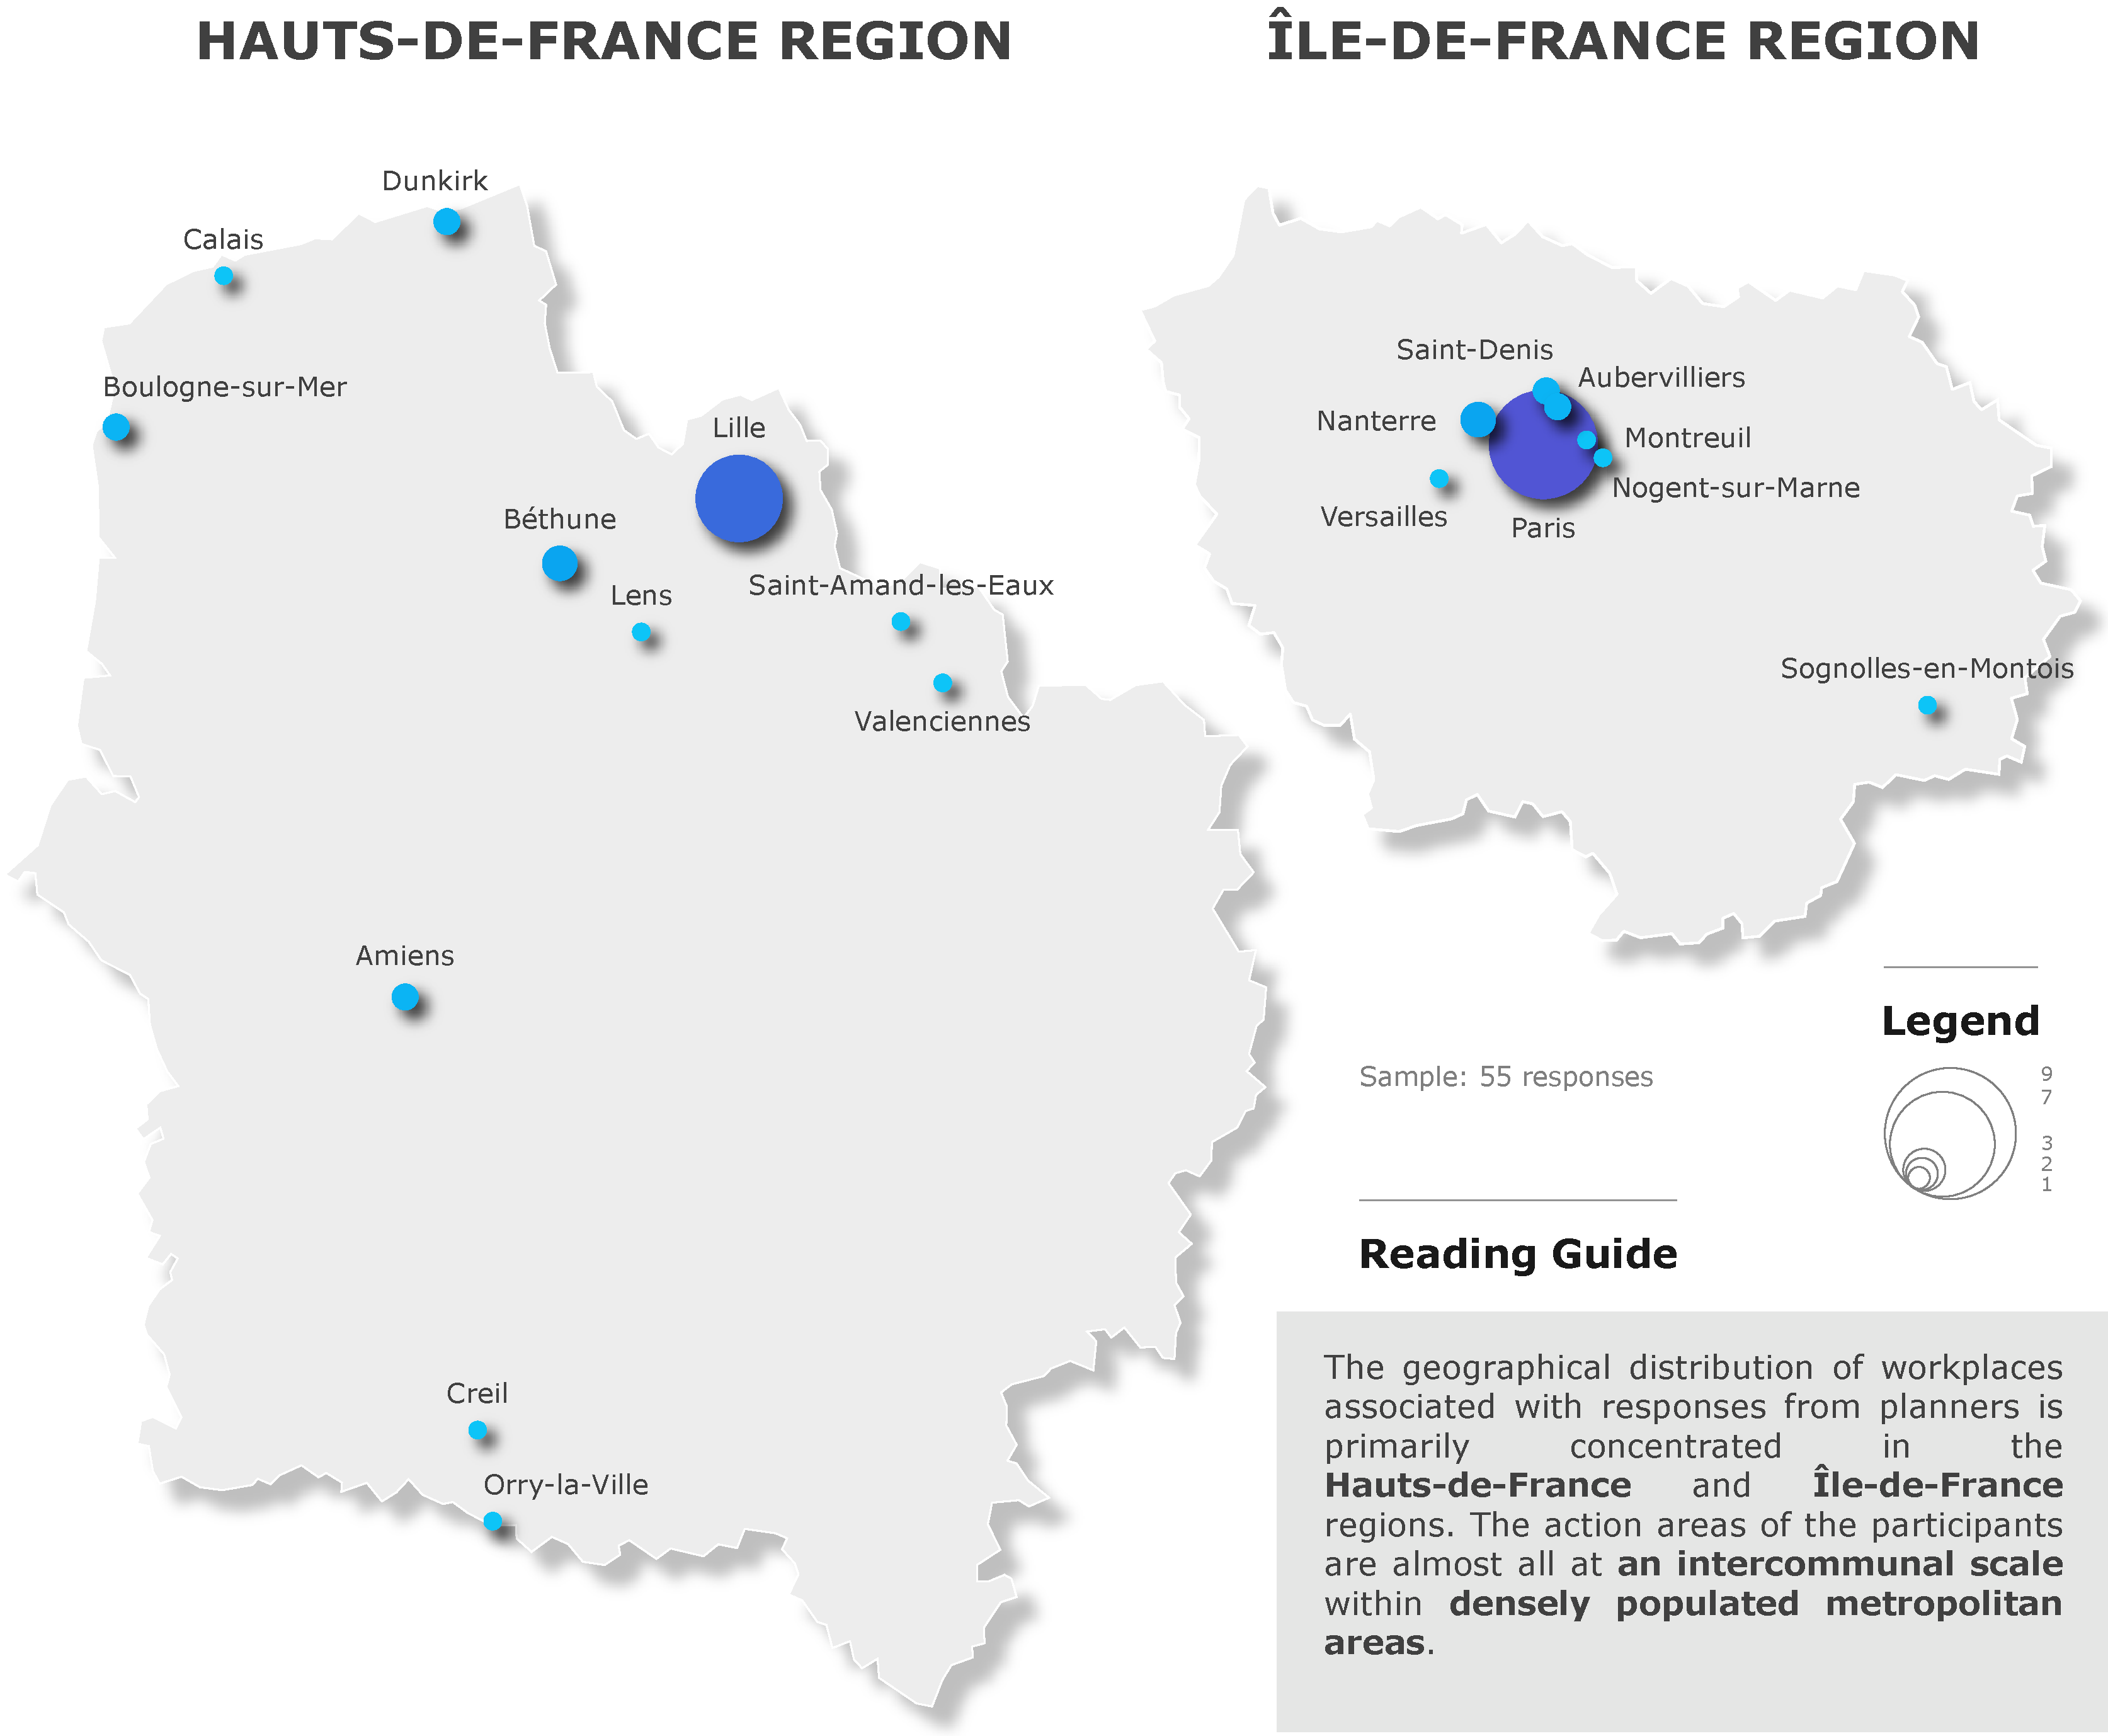
\includegraphics[width=1\columnwidth]{src/Figures/Chap-6/EN_NPART_Carte_lieu_travail_urbanistes.pdf}}
        \vspace{5pt}
        \begin{flushright}\scriptsize{
        Realization: \textcolor{blue}{Dylan Moinse (2024)}
        \\
        Authors: \textsl{NPART} research project
        }\end{flushright}
    \end{carte}

    % Structure and Method
Initially, participants were asked to rank the predefined parameters in our model, after which they were given the opportunity to propose new ones or reject certain presented indicators. Finally, they were prompted to detail their professional and personal profiles. The multicriteria decision-making technique used is based on the \acrfull{BWM}, or the Best-Worst Method.\footnote{~
    The \acrfull{BWM} is an evaluation method that gathers preferences by inviting participants to rank a series of items, which they must judge from most to least important, based on perceived relative utility. This technique has been applied by \textcolor{blue}{\textcite[8]{groenendijk_incorporating_2018}}\index{Groenendijk, Laura|pagebf}\index{Rezaei, Jafar|pagebf}\index{Almeida Correia, Gonçalo Homem de|pagebf} within the \acrshort{NPM} framework.
}, and was developed to determine the relative weights of criteria based on the preferences expressed by decision-makers. The respondent thus identifies the indicator they consider most important (\Commas{the best}) and the one they deem least relevant (\Commas{the worst}). This method takes shape through the prioritization of factors along the three main axes: node, place, and connections. The \textsl{LimeSurvey} platform offers the advantage of an interactive interface, facilitating the entry of variable lists. In terms of analysis type, the evaluation was conducted using the \acrshort{IEW} method to ease comparison with statistical weighting. To enrich the participatory nature of the survey, a series of open-ended questions was also included to encourage planners to propose indicators potentially missing from the initial list and to make recommendations to better guide the strategic thinking on the directions of our research project. Lastly, questions were asked about their training and specialization, their professions, the type and name of their professional organizations, their areas of intervention, the duration of their professional experience, as well as their places of residence and work and their mobility habits.%%Translated%%

    % Sample Description
A total of 55 responses were collected from professionals working in the fields of urban planning and/or mobility, after applying data cleaning and filtering processes. Among them, 22 reside in and/or work in the Hauts-de-France region, while 4 reside in and/or work in a neighboring country (see \hyperref[fig-chap6:localisation-travail-amenageurs-interroges]{Map~\ref{fig-chap6:localisation-travail-amenageurs-interroges}}, page~\pageref{fig-chap6:localisation-travail-amenageurs-interroges}). The majority of respondents primarily use public transportation, with some alternating with light individual mobility or walking, which legitimizes their positions both from the perspective of their knowledge and expertise as well as from their daily user experience. However, it should be noted that participants located in the studied region generally rely on automobiles, especially outside the Lille metropolitan area. To our knowledge, the formation of a final sample of 55 respondents for the weighting of criteria in an \acrshort{NPM} is one of the largest surveys conducted to date, surpassing the 30 planners surveyed by \textcolor{blue}{\textcite[247]{ibrahim_measuring_2023}}\index{Ibrahim, Sara|pagebf}\index{Ayad, Hany|pagebf}\index{Turki, Eslam|pagebf}\index{Saadallah, Dina|pagebf} in Alexandria, and the 36 urban planners surveyed by \textcolor{blue}{\textcite[274]{li_transit_2019}}\index{Li, Zekun|pagebf}\index{Han, Zixuan|pagebf}\index{Xin, Jing|pagebf}\index{Luo, Xin|pagebf}\index{Su, Shiliang|pagebf}\index{Weng, Min|pagebf} in Shanghai.%%Translated%%

    % Transition
After detailing the methodology adopted for the extraction, validation, clustering, and classification of data, we now turn our attention to the results derived from the application of the \acrshort{NPART}. To improve the readability of the analysis and focus our efforts, we chose to focus our study on a specific case, based on two precise typologies: a comparison of pedestrian and cyclist isochrones (\(PI\) and \(CI\)) using the \acrshort{IEW} method for variable weighting, while excluding the weighting defined by planners. This analysis focuses on morning peak hours to capture critical periods of network use and congestion (\(RT_{2}\)), using the k-means algorithm for clustering. By concentrating our attention on these specific parameters, we aim to provide clear and interpretable results. The next section presents the results obtained through the application of \acrshort{NPART} under these conditions, discussing the implications of the relative influences of each indicator, the station locations, and the identified clusters.%%Translated%%

    % ___________________________________________
    % 6.4.
    \newpage
    \needspace{1\baselineskip} % Reserve space
    \sectionheader{Potential of \textsl{Micromobility-friendly Transit-Oriented Development}}
\section{Potential of a \textsl{Micromobility-friendly Transit-Oriented Development}
    \label{chap6:resultats-modele}
    }

    % Introduction
Once the model calibration parameters are established and the methodological protocol outlined, we propose to present the statistical results derived from its application. First, we focus on identifying the most influential criteria for increasing rail traffic, the main goal of \acrshort{TOD}. Based on this analysis, we update the priority components on which public policies should focus to achieve the concept of \acrshort{M-TOD} (see the \hyperref[chap6:results-influence-indicateurs]{section on defining rail-oriented urbanism supported by lightweight individual mobility}, page~\pageref{chap6:results-influence-indicateurs}). Next, we proceed to an evaluation of each station and its urban environment, positioning them within the diagram proposed by the model, to determine whether these entities are in a state of \Commas{equilibrium} or, on the contrary, exhibit a \Commas{certain imbalance} (see the \hyperref[chap6:results-caracterisation-gares]{section on the evaluation of the regional rail network}, page~\pageref{chap6:results-caracterisation-gares}). Finally, this analysis is enriched by a classification task that helps identify strategic stops with potential for development (see the \hyperref[chap6:results-classification-gares]{section on classifying stations and station neighborhoods based on different geographical areas}, page~\pageref{chap6:results-classification-gares}).%%Translated%%

    % 6.4.1.
    \needspace{1\baselineskip} % Reserve space
\subsection{Influence of the Parameters defining a \textsl{Micromobility-friendly Transit-Oriented Development}
    \label{chap6:results-influence-indicateurs}
    }

    % Introduction
The urban planning concept that we strive to formalize, a \acrfull{M-TOD}, is presented as a strategic response aimed at promoting the integration of lightweight individual mobility into rail infrastructure and the urban system. The analysis of the indicators influencing station attendance serves as a lever to understand the mechanisms underlying their attractiveness and, by extension, their potential to drive positive dynamics in transportation systems and urban development. This subsection explores the influence of nodal, urban, and local accessibility parameters on mobility demand, while incorporating the perceptions of urban planning stakeholders. By cross-referencing statistical results with the representations of planners, the goal is to reveal points of convergence and divergence, in order to propose a factual vision of the priorities to be adopted in \acrshort{TOD} planning strategies.%%Translated%%

    % 6.4.1.1.
    \needspace{1\baselineskip} % Reserve space
\subsubsection*{Effects of Rail Service Quality on Transit Demand
    \label{chap6:results-influence-indicateurs-node}
    }

    % Influence of Node Indicators
From the perspective of station service levels, attendance is primarily determined by the frequency of the \acrshort{HST} network, both on weekdays (\(N_{1}\)) and on weekends (\(N_{2}\)), according to the entropy-weighted method (see \hyperref[table-chap6:influence-indicateurs-node]{Table~\ref{table-chap6:influence-indicateurs-node}}, page~\pageref{table-chap6:influence-indicateurs-node} and \hyperref[fig-chap6:resultats-poids-iew-statistiques]{Figure~\ref{fig-chap6:resultats-poids-iew-statistiques}}, page~\pageref{fig-chap6:resultats-poids-iew-statistiques}). Factors related to the frequency of rail connections (from \(N_{1}\) to \(N_{4}\)) are also prominently featured in the criteria assessed by urban planners. Next come the connectivity of stations within the network, evaluated through proximity centrality (\(N_{11}\)) and centrality degree (\(N_{9}\)), which positively influence station attendance. In contrast, the range of service hours (\(N_{5}\) and \(N_{6}\)), as well as access to urban centers (from \(N_{13}\) to \(N_{16}\)) and intermediary centrality (\(N_{10}\)), have a lesser influence, although their importance is often overestimated by planners. Furthermore, planners place little emphasis on the number of services per station (\(N_{8}\)) or the degree of centrality (\(N_{9}\)), even though these are key indicators.%%Translated%%

    % Tableau Influence des indicateurs Node
% Table Influence of Node Indicators
%%Translated%%
    \begin{table}[h!]
    \centering
    \renewcommand{\arraystretch}{1.5}
    \resizebox{\columnwidth}{!}{
    \begin{tabular}{p{0.08\columnwidth}p{0.5\columnwidth}p{0.21\columnwidth}p{0.21\columnwidth}}
        %\hline
    \rule{0pt}{15pt} \small{\textbf{\textcolor{blue}{ID}}} & \small{\textbf{\textcolor{blue}{Indicator}}} & \small{\textbf{\textcolor{blue}{Statistics}}} & \small{\textbf{\textcolor{blue}{Perception}}}\\
        \hline
\small{\(N_{1}\)} & \small{\acrshort{HST} network frequency, on weekdays} & \underline{\small{\textbf{0.264}} (2\textsuperscript{nd})} & \underline{\small{\textbf{0.375}} (1-4\textsuperscript{th})}\\
\small{\(N_{2}\)} & \small{\acrshort{HST} network frequency, on weekends} & \underline{\small{\textbf{0.266}} (1\textsuperscript{st})} & \underline{\small{\textbf{0.375}} (1-4\textsuperscript{th})}\\
\small{\(N_{3}\)} & \small{\acrshort{TER} network frequency, on weekdays} & \small{\textbf{0.034} (7\textsuperscript{th})} & \underline{\small{\textbf{0.375}} (1-4\textsuperscript{th})}\\
\small{\(N_{4}\)} & \small{\acrshort{TER} network frequency, on weekends} & \small{\textbf{0.039} (6\textsuperscript{th})} & \underline{\small{\textbf{0.375}} (1-4\textsuperscript{th})}\\
\small{\(N_{5}\)} & \small{Time span, on weekdays} & \small{\textbf{0.001} (16\textsuperscript{th})} & \small{\textbf{0.082} (11-12\textsuperscript{th})}\\
\small{\(N_{6}\)} & \small{Time span, on weekends} & \small{\textbf{0.009} (14\textsuperscript{th})} & \small{\textbf{0.082} (11-12\textsuperscript{th})}\\
\small{\(N_{7}\)} & \small{Commercial speed} & \small{\textbf{0.015} (9\textsuperscript{th})} & \small{\textbf{0.067} (14\textsuperscript{th})}\\
\small{\(N_{8}\)} & \small{Number of directions} & \small{\textbf{0.068} (5\textsuperscript{th})} & \small{\textbf{0.035} (16\textsuperscript{th})}\\
\small{\(N_{9}\)} & \small{Degree of centrality} & \underline{\small{\textbf{0.077}} (4\textsuperscript{th})} & \small{\textbf{0.057} (15\textsuperscript{th})}\\
\small{\(N_{10}\)} & \small{Intermediary centrality} & \small{\textbf{0.011} (12\textsuperscript{th})} & \small{\textbf{0.134} (5\textsuperscript{th})}\\
\small{\(N_{11}\)} & \small{Proximity centrality} & \underline{\small{\textbf{0.152}} (3\textsuperscript{rd})} & \small{\textbf{0.093} (6\textsuperscript{th})}\\
\small{\(N_{12}\)} & \small{Number of stations accessible within one hour} & \small{\textbf{0.019} (8\textsuperscript{th})} & \small{\textbf{0.067} (13\textsuperscript{th})}\\
\small{\(N_{13}\)} & \small{Number of stations to access Euralille} & \small{\textbf{0.010} (13\textsuperscript{th})} & \small{\textbf{0.090} (7-10\textsuperscript{th})}\\
\small{\(N_{14}\)} & \small{Travel time to access Euralille} & \small{\textbf{0.014} (10\textsuperscript{th})} & \small{\textbf{0.090} (7-10\textsuperscript{th})}\\
\small{\(N_{15}\)} & \small{Number of stations to access Châtelet} & \small{\textbf{0.014} (11\textsuperscript{th})} & \small{\textbf{0.090} (7-10\textsuperscript{th})}\\
\small{\(N_{16}\)} & \small{Travel time to access Châtelet} & \small{\textbf{0.007} (15\textsuperscript{th})} & \small{\textbf{0.090} (7-10\textsuperscript{th})}\\
        \hline
        \end{tabular}}
    \caption{Relative influence, by entropy, of independent indicators related to service level (\(N\)) on station ridership.}
    \label{table-chap6:influence-indicateurs-node}
        \vspace{5pt}
        \begin{flushleft}\scriptsize{
        \textcolor{blue}{Reading Guide:} \acrshort{HST} network frequency on weekends (\(N_{2}\)) statistically explains 20.6\% of station ridership, compared to 37.5\% according to planners.
        }\end{flushleft}
        \begin{flushright}\scriptsize{
        Realization: \textcolor{blue}{Dylan Moinse (2024)}
        \\
        Authors: \acrshort{NPART} Research Project
        }\end{flushright}
        \end{table}%%Rédigé%%

    % Literature
In light of previous \acrshort{NPM} models, \textcolor{blue}{\textcite[8]{cummings_does_2022}}\index{Cummings, Christopher|pagebf}\index{Mahmassani, Hani|pagebf} established that the number of \textsl{Amtrak} services per week in the United States is the most influential variable in the various scenarios analyzed. Similarly, \textcolor{blue}{\textcite[5]{caset_integrating_2020}}\index{Caset, Freke|pagebf}\index{Blainey, Simon|pagebf}\index{Derudder, Ben|pagebf}\index{Boussauw, Kobe|pagebf}\index{Witlox, Frank|pagebf} observed that a 1\% increase in the frequency of \acrshort{TER} services in Flanders, Belgium, leads to a 0.6\% increase in rail network ridership. However, they also determined that the degree of centrality is an even more decisive indicator: a 1\% increase in its value tends to raise station attendance by 2\%. In this regard, \textcolor{blue}{\textcite[11]{amini_pishro_node_2022}}\index{Amini Pishro, Ahad|pagebf}\index{L'Hostis, Alain|pagebf}\index{Chen, Dong|pagebf}\index{Chen, Mojdeh|pagebf}\index{Amini Pishro, Mojdeh|pagebf}\index{Zhang, Zhengrui|pagebf}\index{Li, Jun|pagebf}\index{Zhao, Yuandi|pagebf}\index{Zhang, Lili|pagebf} identified the degree of centrality among the seven most influential indicators for stimulating passenger volume in Chengdu, China. Similarly, \textcolor{blue}{\textcite[9]{cao_coordination_2020}}\index{Cao, Zhejing|pagebf}\index{Asakura, Yasuo|pagebf}\index{Tan, Zongbo|pagebf} highlighted the degree of centrality, as well as the number of \textsl{express} lines, as the two most determining variables for intensifying flows in Tokyo, Japan.%%Translated%%

    % Figure IEW Statistics Weighting
    \begin{figure}[h!]\vspace*{4pt}
        \caption{Statistical influence of indicators on station attendance, at the pedestrian and cycling scale.}
        \label{fig-chap6:resultats-poids-iew-statistiques}
        \centerline{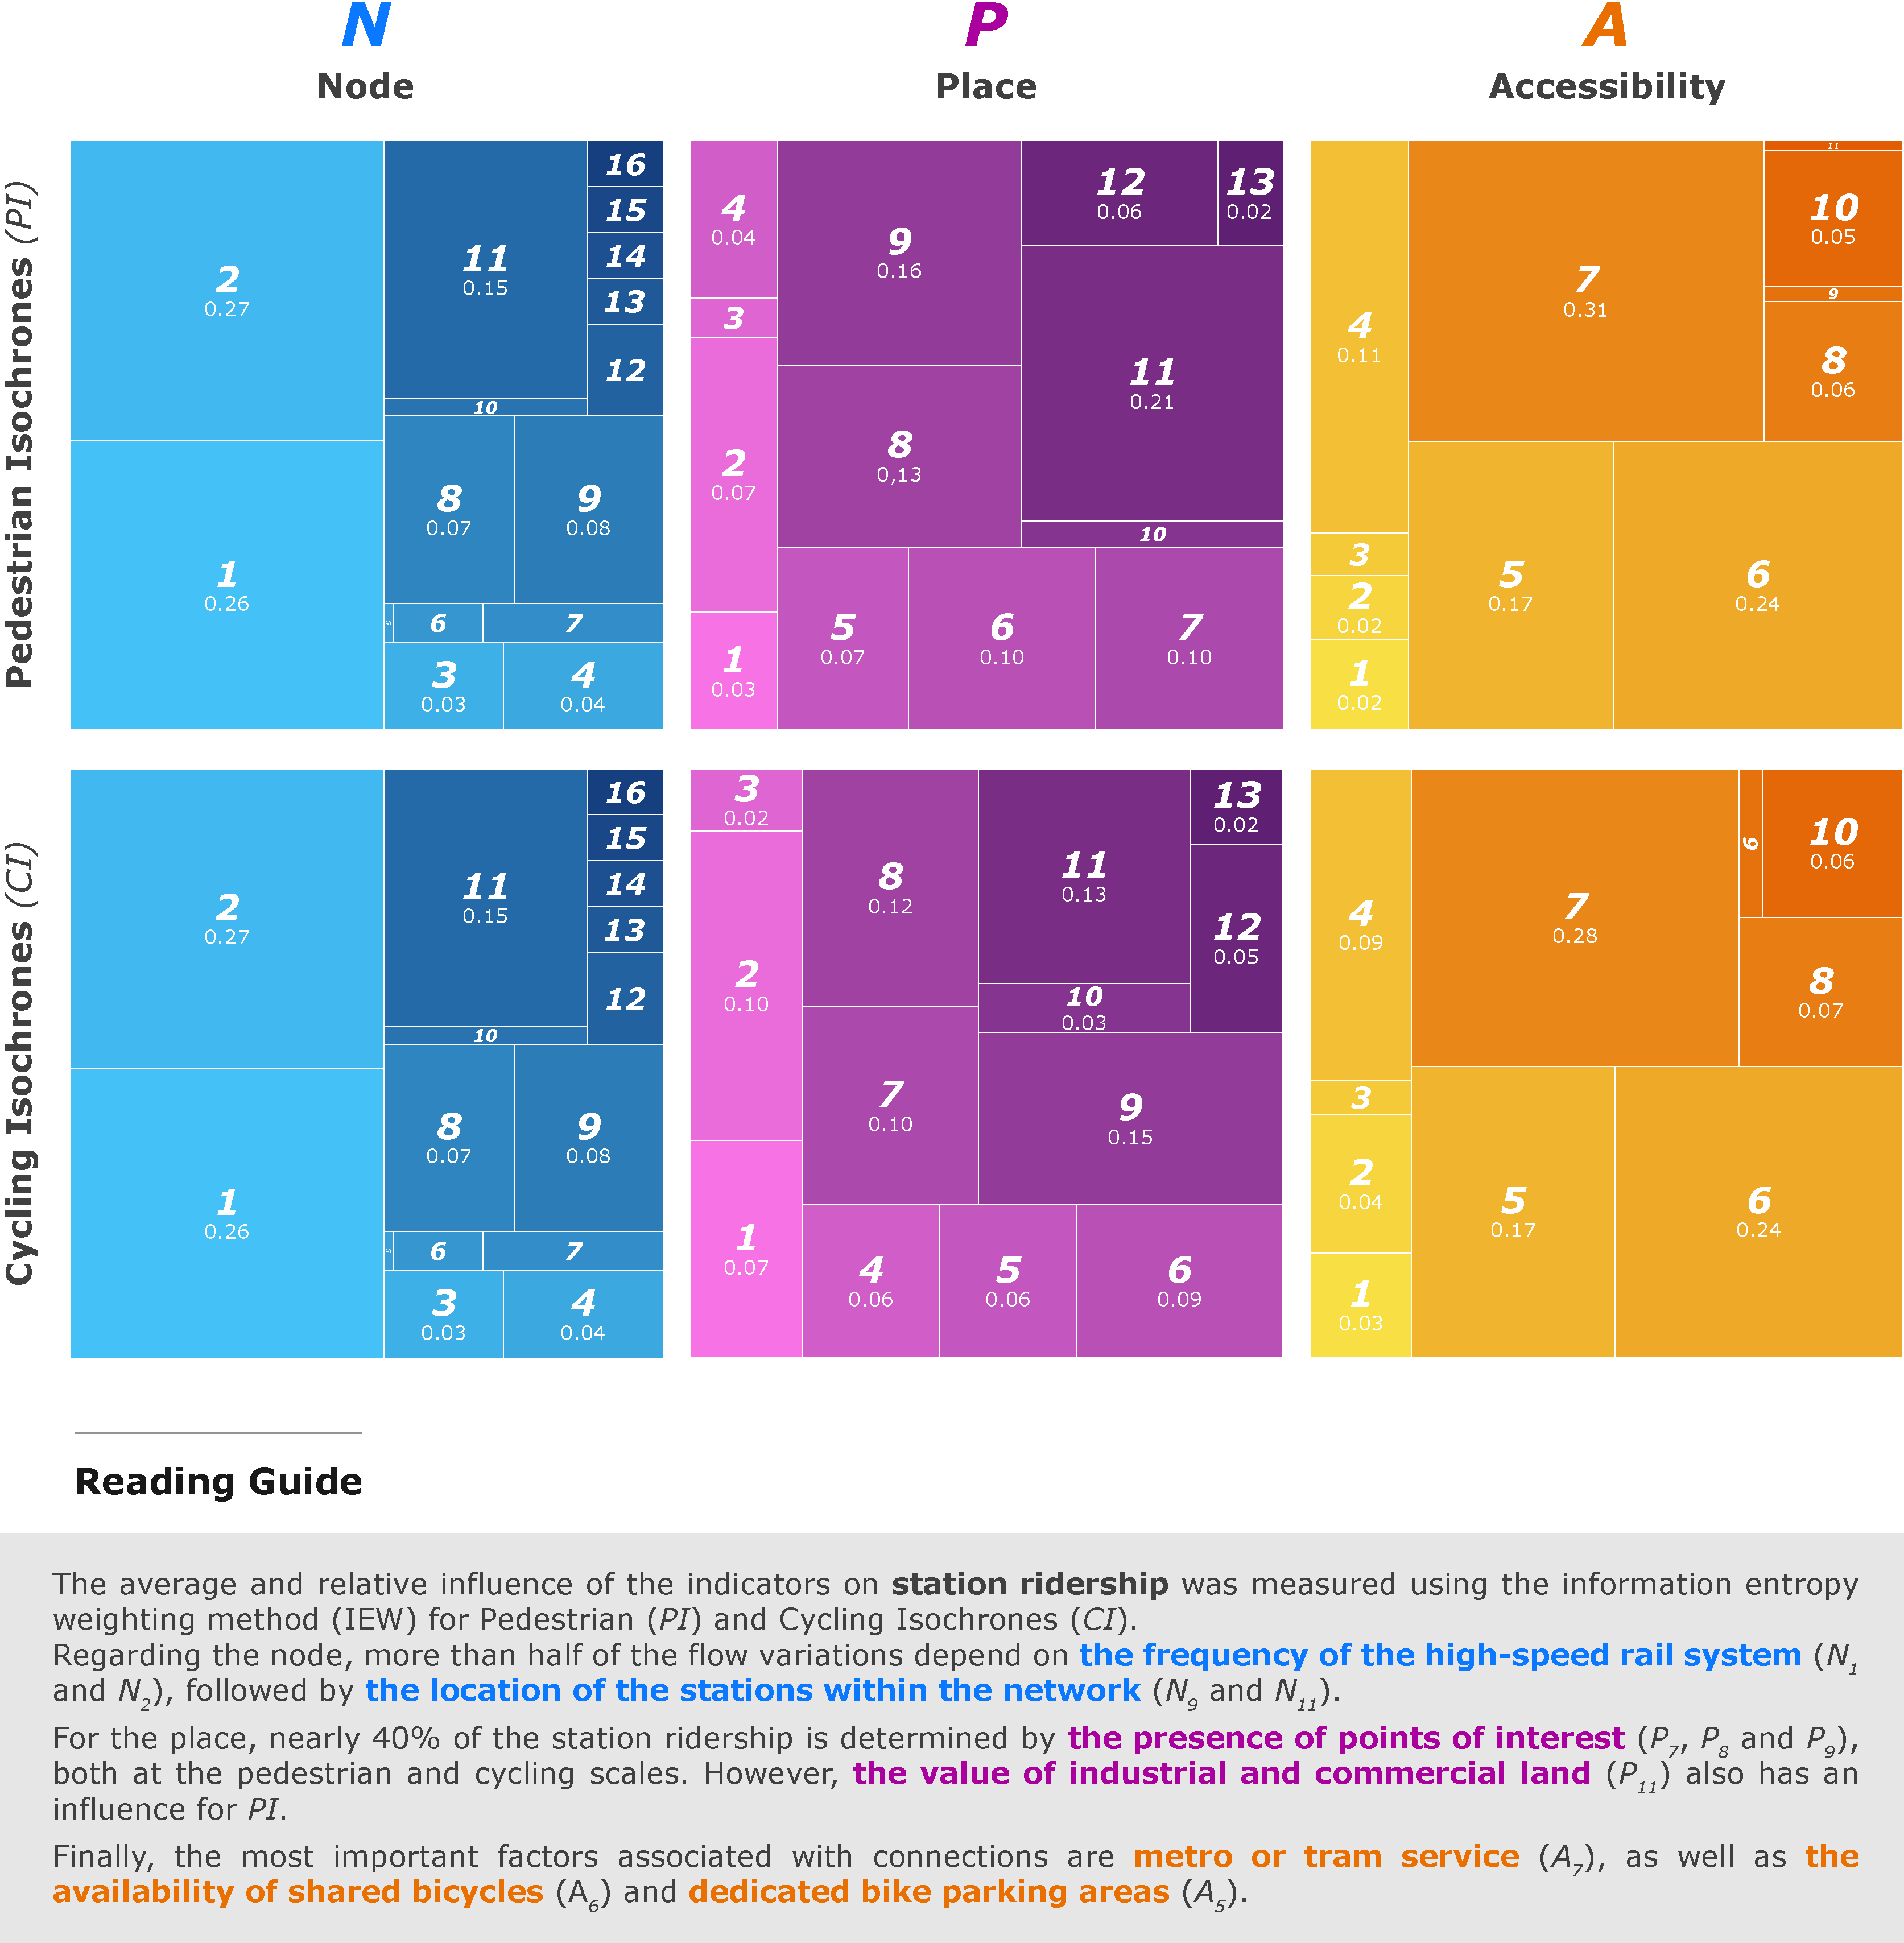
\includegraphics[width=1\columnwidth]{src/Figures/Chap-6/EN_NPART_Poids_Statistiques_IEW_Indicateurs.pdf}}
        \vspace{5pt}
        \begin{flushright}\scriptsize{
        Realization: \textcolor{blue}{Dylan Moinse (2024)}
        \\
        Authors: \acrshort{NPART} Research Project
        }\end{flushright}
    \end{figure}

    % Discussion on the influence of Node Indicators
The fundamental role of the frequency of rail connections, both statistically and in terms of planning objectives, illustrates how this indicator can enhance the attractiveness of stations. At the same time, the strategic position of the node within the networks, highlighted by the need for relatively high proximity centrality and centrality degree, underscores the importance of connections within the network. Indeed, proximity centrality indicates that the station is located close to various nodal points, facilitating intermodal travel, while the degree of centrality confirms the station's role as a key node in the transport network. It should be noted that the statistical analysis emphasizes the importance of the degree of centrality, whereas planning and transport professionals assign it less importance. In contrast, the measure of intermediation, which plays a secondary role, is overemphasized by these same stakeholders, who consider it a far more decisive factor. These observations highlight the role of the concept of \Commas{network} in the dynamics of \acrshort{TOD}: this suggests that the issue of \acrshort{TOD} should not be limited to the immediate vicinity of each station, namely its immediate urban environment, as might be suggested by some reductive analyses \textcolor{blue}{\autocite[10]{cerema_articuler_2015}}\index{Cerema@\textsl{Cerema}|pagebf}. On the contrary, a multi-scale approach should be adopted, simultaneously considering the different spatial dimensions of the transport network and the urban system \textcolor{blue}{\textcite[11]{cervero_transit_1998}}\index{Cervero, Robert|pagebf}. The gap between the assessment of stakeholders and the actual impact of the rail network on station attendance, as well as their tendency to overestimate the role of rail network intermediation, echoes the conclusions of Wendy \textcolor{blue}{\autocite[79]{tan_pursuing_2013}}\index{Tan, Wendy|pagebf}\index{Bertolini, Luca|pagebf}\index{Janssen-Jansen, Leonie|pagebf}'s doctoral thesis on the \Commas{lack of knowledge of public transport specifics by urban planners} (\textsl{culture of public transport is missing}). We can conclude that the main factors explaining station attendance involve strengthening their \Commas{nodality}\footnote{~
    The concept of \Commas{nodality} refers to \Commas{\textsl{the set of characteristics related to the morphology, functioning, and dynamics of transport nodes} [\dots]} \textcolor{blue}{\autocite[5]{bavoux_nodalite_2005}}\index{Bavoux, Jean-Jacques|pagebf}. The author also proposes the term \Commas{nodosity} to describe the various aggregation phenomena that may accompany a circulatory nodality \textcolor{blue}{\autocite[13]{bavoux_nodalite_2005}}\index{Bavoux, Jean-Jacques|pagebf}.
} related to interactions between centrality, accessibility, and attractiveness at different scales \textcolor{blue}{\autocite[13]{bavoux_nodalite_2005}}\index{Bavoux, Jean-Jacques|pagebf}. It is therefore the responsibility of mobility infrastructure managers to ensure optimal integration of stations into the regional rail network. This integration could involve maximizing service frequency and improving station connectivity.%%Translated%%

    % 6.4.1.2.
    \needspace{1\baselineskip} % Reserve space
\subsubsection*{Effects of Urban Development Degree on Transit Demand
    \label{chap6:results-influence-indicateurs-place}
    }

    % Influence of Place Indicators
From a statistical standpoint, the urban development indicators that have the greatest influence on station attendance include the value of real estate for commercial and industrial activities (\(P_{11}\)), \acrshort{POIs} of \Commas{higher} and \Commas{intermediate} categories (\(P_{9}\) and \(P_{8}\)), land use for green spaces (\(P_{6}\)), and employment density (\(P_{2}\)), as illustrated in \hyperref[table-chap6:influence-indicateurs-place]{Table~\ref{table-chap6:influence-indicateurs-place}} (page~\pageref{table-chap6:influence-indicateurs-place}) and \hyperref[fig-chap6:resultats-poids-iew-statistiques]{Figure~\ref{fig-chap6:resultats-poids-iew-statistiques}} (page~\pageref{fig-chap6:resultats-poids-iew-statistiques}). In practice, a distinction is made between pedestrian (\(PI\)) and cycling (\(CI\)) areas around stations, with employment and population densities (\(P_{1}\)) playing a more significant role in the \Commas{secondary area}. From the perspective of urban planners, land use dominated by commercial activities (\(P_{4}\)) and the presence of facilities and services (from \(P_{7}\) to \(P_{9}\)) are considered crucial. In contrast, the land value receives little attention from urban development stakeholders, which reveals a strong emphasis on commercial and service functions in terms of urban integration, while also reflecting a tendency to underestimate the importance of real estate value.%%Translated%%

    % Tableau Influence des indicateurs Place
% Table Influence of Place Indicators
%%Translated%%
    \begin{table}[h!]
    \centering
    \renewcommand{\arraystretch}{1.5}
    \resizebox{\columnwidth}{!}{
    \begin{tabular}{p{0.08\columnwidth}p{0.38\columnwidth}p{0.18\columnwidth}p{0.18\columnwidth}p{0.18\columnwidth}}
        %\hline
    \rule{0pt}{15pt} \small{\textbf{\textcolor{blue}{ID}}} & \small{\textbf{\textcolor{blue}{Indicator}}} & \small{\textbf{\textcolor{blue}{\(PI\)*}}} & \small{\textbf{\textcolor{blue}{\(CI\)*}}} & \small{\textbf{\textcolor{blue}{Perception}}}\\
        \hline
\small{\(P_{1}\)} & \small{Population density} & \small{\textbf{0.035} (10\textsuperscript{th})} & \small{\textbf{0.072} (7\textsuperscript{th})} & \small{\textbf{0.097} (7\textsuperscript{th})}\\
\small{\(P_{2}\)} & \small{Employment density} & \small{\textbf{0.068} (7\textsuperscript{th})} & \underline{\small{\textbf{0.104}} (4\textsuperscript{th})} & \small{\textbf{0.102} (6\textsuperscript{th})}\\
\small{\(P_{3}\)} & \small{Residential function} & \small{\textbf{0.007} (13\textsuperscript{th})} & \small{\textbf{0.023} (12\textsuperscript{th})} & \small{\textbf{0.087} (11\textsuperscript{th})}\\
\small{\(P_{4}\)} & \small{Commercial function} & \small{\textbf{0.039} (9\textsuperscript{th})} & \small{\textbf{0.062} (9\textsuperscript{th})} & \underline{\small{\textbf{0.119}} (1\textsuperscript{st})}\\
\small{\(P_{5}\)} & \small{Industrial and office function} & \small{\textbf{0.070} (6\textsuperscript{th})} & \small{\textbf{0.062} (8\textsuperscript{th})} & \small{\textbf{0.089} (10\textsuperscript{th})}\\
\small{\(P_{6}\)} & \small{Presence of green spaces} & \underline{\small{\textbf{0.096}} (4\textsuperscript{th})} & \small{\textbf{0.094} (6\textsuperscript{th})} & \small{\textbf{0.105} (5\textsuperscript{th})}\\
\small{\(P_{7}\)} & \small{\acrshort{POIs} of \Commas{proximity}} & \small{\textbf{0.096} (5\textsuperscript{th})} & \small{\textbf{0.096} (5\textsuperscript{th})} & \underline{\small{\textbf{0.115}} (2-4\textsuperscript{th})}\\
\small{\(P_{8}\)} & \small{\acrshort{POIs} \Commas{intermediate}} & \underline{\small{\textbf{0.131}} (3\textsuperscript{rd})} & \underline{\small{\textbf{0.118}} (3\textsuperscript{rd})} & \underline{\small{\textbf{0.115}} (2-4\textsuperscript{th})}\\
\small{\(P_{9}\)} & \small{\acrshort{POIs} \Commas{superior}} & \underline{\small{\textbf{0.160}} (2\textsuperscript{nd})} & \underline{\small{\textbf{0.153}} (1\textsuperscript{st})} & \underline{\small{\textbf{0.115}} (2-4\textsuperscript{th})}\\
\small{\(P_{10}\)} & \small{Value of residential locations} & \small{\textbf{0.018} (11\textsuperscript{th})} & \small{\textbf{0.026} (11\textsuperscript{th})} & \small{\textbf{0.094} (8\textsuperscript{th})}\\
\small{\(P_{11}\)} & \small{Value of activity locations} & \underline{\small{\textbf{0.206}} (1\textsuperscript{st})} & \underline{\small{\textbf{0.130}} (2\textsuperscript{nd})} & \small{\textbf{0.012} (13\textsuperscript{th})}\\
\small{\(P_{12}\)} & \small{Share of social housing} & \small{\textbf{0.055} (8\textsuperscript{th})} & \small{\textbf{0.046} (10\textsuperscript{th})} & \small{\textbf{0.092} (9\textsuperscript{th})}\\
\small{\(P_{13}\)} & \small{Average household income} & \small{\textbf{0.018} (12\textsuperscript{th})} & \small{\textbf{0.016} (13\textsuperscript{th})} & \small{\textbf{0.087} (12\textsuperscript{th})}\\
        \hline
        \end{tabular}}
    \caption{Relative influence, by entropy, of independent indicators related to urban integration (\(P\)) on station ridership.}
    \label{table-chap6:influence-indicateurs-place}
        \vspace{5pt}
        \begin{flushleft}\scriptsize{
        \textcolor{blue}{Note:} \(PI\) and \(CI\) statistics correspond to values specific to pedestrian and cycling isochrones.
        \\
        \textcolor{blue}{Reading Guide:} The value of activity locations (\(P_{11}\)) statistically explains 20.6\% and 13.0\% of station ridership for pedestrian (\(PI\)) and cycling (\(CI\)) areas. The expected effects of this variable are only 1.2\% according to planners.
        }\end{flushleft}
        \begin{flushright}\scriptsize{
        Realization: \textcolor{blue}{Dylan Moinse (2024)}
        \\
        Authors: \acrshort{NPART} Research Project
        }\end{flushright}
        \end{table}%%Rédigé%%

    % Literature
These results are consistent with the observations of \textcolor{blue}{\textcite[11]{amini_pishro_node_2022}}\index{Amini Pishro, Ahad|pagebf}\index{Yang, Qihong|pagebf}\index{Zhang, Shiquan|pagebf}\index{Amini Pishro, Mojdeh|pagebf}\index{Zhang, Zhengrui|pagebf}\index{Zhao, Yana|pagebf}\index{Postel, Victor|pagebf}\index{Huang, Dengshi|pagebf}\index{Li, WeiYu|pagebf} who indicate that the average price of commercial and office land is positively correlated with station attendance. In contrast, our results differ from those reported by \textcolor{blue}{\textcite[9]{cummings_does_2022}}\index{Cummings, Christopher|pagebf}\index{Mahmassani, Hani|pagebf}, who note a positive correlation between housing prices around stations and station attendance in the United States. As for the \acrshort{POIs}, \textcolor{blue}{\textcite[5]{pezeshknejad_evaluating_2020}}\index{Pezeshknejad, Parsa|pagebf}\index{Monajem, Saeed|pagebf}\index{Mozafari, Hamid|pagebf} find that areas around \acrshort{BRT} stops with a high concentration of \acrshort{POIs} attract more passengers in Tehran, Iran. More generally, land use dominated by commercial and office spaces, as well as employment density, tends to increase the ridership of \textsl{Amtrak} services \textcolor{blue}{\autocite[8]{cummings_does_2022}}\index{Cummings, Christopher|pagebf}\index{Mahmassani, Hani|pagebf}.%%Translated%%

    % Discussion on the influence of Place Indicators
The examination of urban development indicators influencing station attendance highlights the role played by the urban and economic integration of stations and their surroundings within the \acrshort{M-TOD} framework. Commercial and industrial real estate properties, along with the increased presence of \acrshort{POIs} and employment density, emerge as substantial drivers of station attractiveness. However, the low attention given to land value raises questions and suggests a potential imbalance in the consideration of real estate factors. Experts identify the commercial function, while the statistical analysis emphasizes the land values of activity areas. Such underestimation by stakeholders could obscure opportunities for enhancing and financing transport infrastructure and public space development, key elements of the third dimension of \acrshort{NPART}.%%Translated%%

    % 6.4.1.3.
    \needspace{1\baselineskip} % Reserve space
\subsubsection*{Effects of Public Space Management and Local Accessibility on Transit Demand
    \label{chap6:results-influence-indicateurs-accessibility}
    }

    % Influence of Accessibility Indicators
Regarding public space management and local accessibility, statistically, it is primarily the issue of the \Commas{first and last miles} that predominantly influences station attendance, as shown in \hyperref[table-chap6:influence-indicateurs-accessibility]{Table~\ref{table-chap6:influence-indicateurs-accessibility}} (page~\pageref{table-chap6:influence-indicateurs-accessibility}) and \hyperref[fig-chap6:resultats-poids-iew-statistiques]{Figure~\ref{fig-chap6:resultats-poids-iew-statistiques}} (page~\pageref{fig-chap6:resultats-poids-iew-statistiques}). More specifically, we find the service of urban rail public transport networks (\(A_{7}\)) and three major aspects of the \Commas{bike system} \textcolor{blue}{\autocites[169]{heran_retour_2015}[]{heran_systeme_2001}}\index{Héran, Frédéric|pagebf}, namely the presence of \acrshort{PBS} services (\(A_{6}\)) as well as the provision of bike parking spaces (\(A_{5}\)) and a cycling network (\(A_{4}\)). These statistical results highlight the strategic role of \gls{intermodality} in the attractiveness of the rail network and stations at the local level. These observations are followed by responses gathered from local experts who ranked the importance of the pedestrian network (\(A_{1}\)), bike parking (\(A_{5}\)), motorized speed (\(A_{9}\)), and the provision of metro and tram services (\(A_{7}\)).%%Translated%%

    % Tableau Influence des indicateurs Accessibility
% Table Influence of Accessibility Indicators
%%Translated%%
    \begin{table}[h!]
    \centering
    \renewcommand{\arraystretch}{1.5}
    \resizebox{\columnwidth}{!}{
    \begin{tabular}{p{0.08\columnwidth}p{0.38\columnwidth}p{0.18\columnwidth}p{0.18\columnwidth}p{0.18\columnwidth}}
        %\hline
    \rule{0pt}{15pt} \small{\textbf{\textcolor{blue}{ID}}} & \small{\textbf{\textcolor{blue}{Indicator}}} & \small{\textbf{\textcolor{blue}{\(PI\)*}}} & \small{\textbf{\textcolor{blue}{\(CI\)*}}} & \small{\textbf{\textcolor{blue}{Perception}}}\\
        \hline
\small{\(A_{1}\)} & \small{Pedestrian network} & \small{\textbf{0.025} (7\textsuperscript{th})} & \small{\textbf{0.027} (8\textsuperscript{th})} & \underline{\small{\textbf{0.120}} (1\textsuperscript{st})}\\
\small{\(A_{2}\)} & \small{Intersection density} & \small{\textbf{0.018} (8\textsuperscript{th})} & \small{\textbf{0.037} (7\textsuperscript{th})} & \small{\textbf{0.086} (7\textsuperscript{th})}\\
\small{\(A_{3}\)} & \small{Spatial efficiency rate} & \small{\textbf{0.012} (9\textsuperscript{th})} & \small{\textbf{0.009} (10\textsuperscript{th})} & \small{\textbf{0.041} (11\textsuperscript{th})}\\
\small{\(A_{4}\)} & \small{Cycling network} & \underline{\small{\textbf{0.110}} (4\textsuperscript{th})} & \underline{\small{\textbf{0.085}} (4\textsuperscript{th})} & \small{\textbf{0.086} (8\textsuperscript{th})}\\
\small{\(A_{5}\)} & \small{Bicycle parking} & \underline{\small{\textbf{0.169}} (3\textsuperscript{rd})} & \underline{\small{\textbf{0.171}} (3\textsuperscript{rd})} & \underline{\small{\textbf{0.115}} (2\textsuperscript{nd})}\\
\small{\(A_{6}\)} & \small{Bike-sharing services} & \underline{\small{\textbf{0.239}} (2\textsuperscript{nd})} & \underline{\small{\textbf{0.244}} (2\textsuperscript{nd})} & \small{\textbf{0.084} (9\textsuperscript{th})}\\
\small{\(A_{7}\)} & \small{Metro and tram services} & \underline{\small{\textbf{0.307}} (1\textsuperscript{st})} & \underline{\small{\textbf{0.284}} (1\textsuperscript{st})} & \underline{\small{\textbf{0.097}} (4\textsuperscript{th})}\\
\small{\(A_{8}\)} & \small{Bus and \acrshort{BRT} services} & \small{\textbf{0.056} (5\textsuperscript{th})} & \small{\textbf{0.068} (5\textsuperscript{th})} & \small{\textbf{0.081} (10\textsuperscript{th})}\\
\small{\(A_{9}\)} & \small{Motorized speed} & \small{\textbf{0.006} (10\textsuperscript{th})} & \small{\textbf{0.009} (9\textsuperscript{th})} & \underline{\small{\textbf{0.106}} (3\textsuperscript{rd})}\\
\small{\(A_{10}\)} & \small{Car parking} & \small{\textbf{0.054} (6\textsuperscript{th})} & \small{\textbf{0.064} (6\textsuperscript{th})} & \small{\textbf{0.094} (5\textsuperscript{th})}\\
\small{\(A_{11}\)} & \small{Motorization rate} & \small{\textbf{0.004} (11\textsuperscript{th})} & \small{\textbf{0.003} (11\textsuperscript{th})} & \small{\textbf{0.088} (6\textsuperscript{th})}\\
        \hline
        \end{tabular}}
    \caption{Relative influence, by entropy, of independent indicators related to local accessibility (\(A\)) on station ridership.}
    \label{table-chap6:influence-indicateurs-accessibility}
        \vspace{5pt}
        \begin{flushleft}\scriptsize{
        \textcolor{blue}{Note~:} \(PI\) and \(CI\) statistics correspond to values specific to pedestrian and cycling isochrones.
        \\
        \textcolor{blue}{Reading Guide:} Metro and tram services (\(A_{7}\)) statistically explain 30.7\% and 28.4\% of station ridership for pedestrian (\(PI\)) and cycling (\(CI\)) zones. The expected effects of this variable are only 9.7\% according to planners.
        }\end{flushleft}
        \begin{flushright}\scriptsize{
        Realization: \textcolor{blue}{Dylan Moinse (2024)}
        \\
        Authors: \acrshort{NPART} Research Project
        }\end{flushright}
        \end{table}%%Rédigé%%

    % Literature
Our observations align with previous research that has examined the interactions between factors influencing local accessibility and station attendance. \textcolor{blue}{\textcite[511]{caset_measuring_2018}}\index{Caset, Freke|pagebf}\index{Vale, David~S.|pagebf}\index{Viana, Cláudia~M.|pagebf} found, through a correlation analysis, a weak association between active modes and other indicators in their model, with the notable exception of the presence of \acrshort{PBS} systems near stations, which is significantly linked to \gls{multimodality}, including bus services, car-sharing, as well as a walkable environment and high population density. In contrast, \textcolor{blue}{\textcite[8]{olaru_place_2019}}\index{Olaru, Doina|pagebf}\index{Moncrieff, Simon|pagebf}\index{McCarney, Gary|pagebf}\index{Sun, Yuchao|pagebf}\index{Reed, Tristan|pagebf}\index{Pattison, Cate|pagebf}\index{Smith, Brett|pagebf}\index{Biermann, Sharon|pagebf} identify a negative relationship between walkability and mobility demand, suggesting that pedestrian and cycling-friendly infrastructure tends to mainly encourage car users to switch to these active modes, rather than promoting train usage. This finding is supported by \textcolor{blue}{\textcite[7]{caset_integrating_2020}}\index{Caset, Freke|pagebf}\index{Blainey, Simon|pagebf}\index{Derudder, Ben|pagebf}\index{Boussauw, Kobe|pagebf}\index{Witlox, Frank|pagebf} who note that the length of pedestrian and cycling infrastructure does not seem to stimulate station attendance, unlike spatial efficiency, i.e., the actual accessible station perimeter. Finally, according to \textcolor{blue}{\textcite[1021]{maheshwari_evaluating_2022}}\index{Maheshwari, Richa|pagebf}\index{Grigolon, Anna|pagebf}\index{Brussel, Mark|pagebf}, the surveyed urban planners place significant value on the development of the pedestrian network as the most crucial criterion in implementing a \acrshort{TOD} project, which also aligns with our findings.%%Translated%%

    % Discussion
In contrast to the trends observed in the previous two dimensions, this third category highlights the relative importance of indicators that are rarely considered, emphasizing the significance of an \acrshort{M-TOD} at all geographical scales, while underscoring the issue of the \Commas{first and last miles} of public transport. The design of public spaces, although secondary, contrasts with the relevance of modes of transport that complement the train, which in turn encourage the development of rail flows. The relative importance of infrastructure and services dedicated to lightweight individual mobility in station neighborhoods illustrates the need for better integration of this intermodal perspective, which is often absent from studies. Furthermore, we can observe that car parking near stations, although playing a moderate role compared to cycling and micromobility, still has a significant influence. This indicates a coexistence of three modal chaining solutions: urban public transport systems, lightweight individual mobility, and private car use. This context reveals a paradox, as it is crucial to reduce both car usage and parking to promote a better modal balance, while avoiding discouraging train use in favor of the car. Such results suggest prioritizing active modes, while maintaining, albeit limited, car access in station neighborhoods, lest market share be lost. Finally, a significant gap remains between the measured impact of the indicators and how urban planners perceive them, with a tendency to overestimate the importance of the pedestrian network and motor vehicle speed limits, and underestimate the importance of bike-sharing and bus services, as well as the cycling network.%%Translated%%

    % 6.4.1.4.
    \needspace{1\baselineskip} % Reserve space
\subsubsection*{Difference in Influence between Actual Urban Factors and their Representation by Stakeholders
    \label{chap6:results-ecarts-influence-indicateurs}
    }

% Representation discrepancies influence indicators
We are able to quantify the discrepancies between statistical regression analyses and the expectations of urban planners, with the goal of developing a transit-oriented urban strategy \acrshort{TOD}. As shown in \hyperref[fig-chap6:ecarts-representation-indicateurs]{Figure~\ref{fig-chap6:ecarts-representation-indicateurs}} (page~\pageref{fig-chap6:ecarts-representation-indicateurs}), the divergences in influence between pedestrian train station areas (\(PI\)) and bicycle-friendly areas (\(CI\)) are minimal. At the station service level, the impact remains similar at the node scale. However, in the \Commas{secondary area}, the importance of land value for industrial, commercial, and office properties (\(P_{11}\)) decreases, while the value of population density (\(P_{1}\)) and employment density (\(P_{2}\)) increases. On the experts' side, opinions vary more widely, revealing more significant disparities. Few indicators clearly stand out in each dimension of the \acrshort{NPART} model. As a result, planning professionals tend to underestimate certain indicators, such as metro and tramway coverage (\(A_{7}\)), the land value of properties dedicated to activities (\(P_{11}\)), and \acrshort{PBS} services (\(A_{6}\)). Conversely, they seem to overestimate the frequency of the \acrshort{TER} network (\(N_{3}\) and \(N_{4}\)), as well as the centrality of intermediation (\(N_{10}\)) and the length of the pedestrian network (\(A_{1}\)). This analysis highlights the need for a reassessment of the criteria used in urban planning to better align planning objectives with data derived from statistical analyses. %%Translated%%

% Figure representation discrepancies indicators
\begin{figure}[h!]\vspace*{4pt}
    \caption{Delayed influence of various indicators between statistical results and planners' representations.}
    \label{fig-chap6:ecarts-representation-indicateurs}
    \centerline{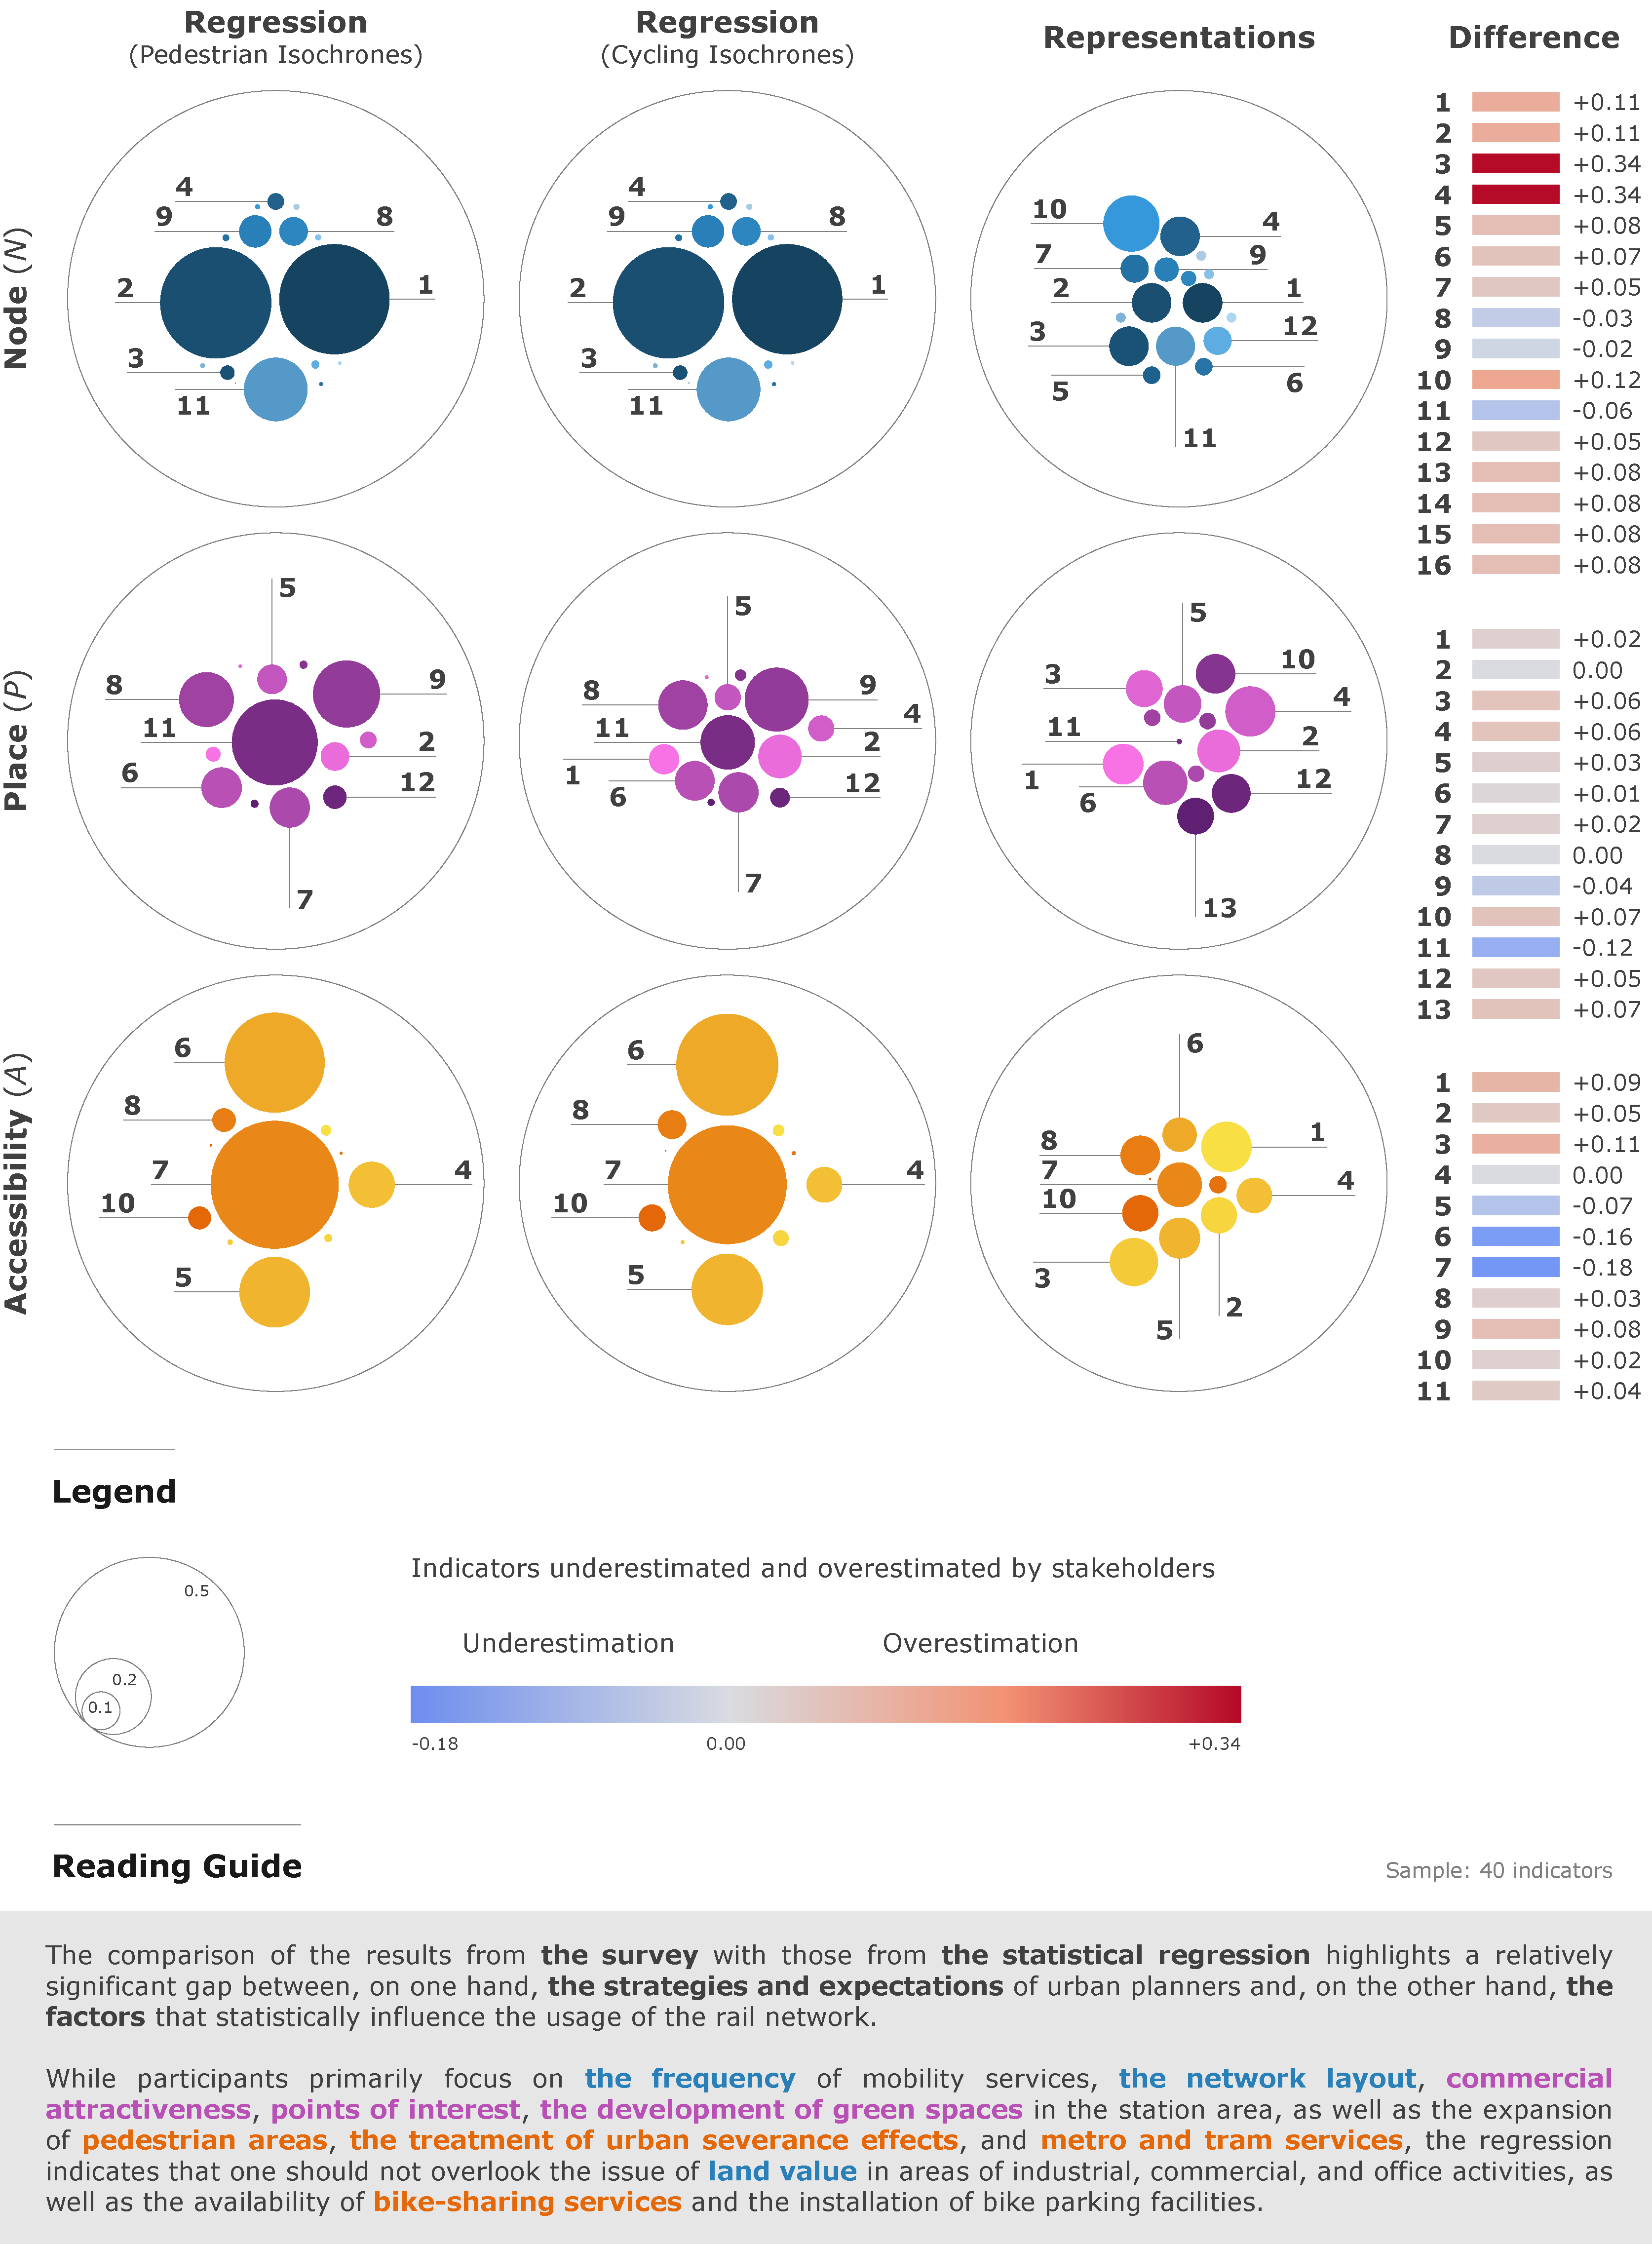
\includegraphics[width=1\columnwidth]{src/Figures/Chap-6/EN_NPART_Confrontation_Poids_Indicateurs.pdf}}
    \vspace{5pt}
    \begin{flushright}\scriptsize{
    Creation: \textcolor{blue}{Dylan Moinse (2024)}
    \\
    Authors: \acrshort{NPART} Research Project
    }\end{flushright}
\end{figure}

% Literature node
In our model, it appears that urban planning actors tend to overestimate the positive impact of rail services on \acrshort{TOD} and \acrshort{M-TOD}, particularly regarding frequency (\(N_{1}\), \(N_{2}\), \(N_{3}\), and \(N_{4}\)), operating hours (\(N_{5}\) and \(N_{6}\)), the nodal position of interconnection (\(N_{10}\)), and direct access to metropolitan areas (\(N_{13}\), \(N_{14}\), \(N_{15}\), and \(N_{16}\)). This finding aligns with the conclusions of \textcolor{blue}{\textcite[41]{lukman_development_2014}}\index{Lukman, Azhari|pagebf}\index{Singh, Yamini Jain|pagebf}, who note that urban planners place more value on rail system-related criteria in a workshop on Arnhem and Nijmegen in the Netherlands. In particular, \textcolor{blue}{\textcite[2430]{kumar_developing_2020}}\index{Kumar,~P. Phani|pagebf}\index{Parida, Manoranjan|pagebf}\index{Sekhar, Ch. Ravi|pagebf} and \textcolor{blue}{\textcite[42]{lukman_development_2014}}\index{Lukman, Azhari|pagebf}\index{Singh, Yamini Jain|pagebf} identify the frequency of services as the most valued aspect by Indian and Dutch planners, while the central location of stations within the network emerges as a key element in Belgium \textcolor{blue}{\autocite[95]{caset_planning_2019}}\index{Caset, Freke|pagebf}, observations that resonate with the results of our own study.%%Translated%%

% Literature - built environment
Regarding the built environment, often prioritized by local experts in the literature \textcolor{blue}{\autocite[41]{lukman_development_2014}}\index{Lukman, Azhari|pagebf}\index{Singh, Yamini Jain|pagebf}, the participants who contributed to the calibration of the \acrshort{NPART} model seem to place less importance on aspects such as density or diversity, which may appear counterintuitive. In contrast, they overestimate the strategic role of the pedestrian network length (\(A_{1}\)), obstacle treatment (\(A_{3}\)), and motorized speed limitations (\(A_{9}\)). These points are also highlighted in the work of \textcolor{blue}{\textcite[2430]{kumar_developing_2020}}\index{Kumar,~P. Phani|pagebf}\index{Parida, Manoranjan|pagebf}\index{Sekhar, Ch. Ravi|pagebf} and in the research report published by \textcolor{blue}{\textcite[19]{transportation_research_board_transit-oriented_2005}}\index{Transportation Research Board@\textsl{Transportation Research Board}|pagebf}\index{National Academies of Sciences, Engineering, and Medicine@\textsl{National Academies of Sciences, Engineering, and Medicine}|pagebf}, where pedestrian-oriented design is considered highly useful by the planners surveyed. However, the results from our questionnaire, cross-referenced with our statistical regression model, show that the latter place less weight on car parking availability or road connectivity, as well as land value or the presence of offices and shops, marking a divergence from the scientific literature \textcolor{blue}{\autocites[19]{transportation_research_board_transit-oriented_2005}[42]{lukman_development_2014}[95]{caset_planning_2019}}\index{Caset, Freke|pagebf}\index{Lukman, Azhari|pagebf}\index{Singh, Yamini Jain|pagebf}\index{Transportation Research Board@\textsl{Transportation Research Board}|pagebf}\index{National Academies of Sciences, Engineering, and Medicine@\textsl{National Academies of Sciences, Engineering, and Medicine}|pagebf}.%%Translated%%

% Transition
The study of the individual influence of each indicator on \acrshort{TOD} at the pedestrian and bicycle scale allowed us to quantify their effects on the attractiveness of train stations and highlight the discrepancies between actual impacts and the representations of designers. To gain a more accurate view of the development potential through public transportation systems in our regional case study, we will focus on evaluating the accessibility of stations and their immediate environment, by examining the interactions between the four dimensions of the \acrshort{NPART} model.%%Translated%%

% 6.4.2.
\needspace{1\baselineskip} % Reserve space
\subsection{Evaluation of the Accessibility of Nodes and Train Station Neighborhoods in the Region
    \label{chap6:results-caracterisation-gares}
    }

% Introduction
The next step involves characterizing the train stations and their surrounding neighborhoods to assess the \Commas{balance} of functions at each station. This subsection specifically focuses on stations classified as \Commas{dependent,} a category that predominates in the studied network. Indeed, these stations are characterized by moderate or low values for at least two of the studied dimensions, indicating a lack of coordination between the quality of the rail network, territorial dynamics, and local connections. This situation reflects areas where mobility demand and the attractiveness of stations remain limited. By relying on three-dimensional graphical representations and weighted descriptive indicators, we aim to deepen our understanding of the factors that limit their development, while positioning them relative to the complementary category of \Commas{accessible} stations. Furthermore, this subsection highlights significant interdependencies between the different dimensions of the \acrshort{NPART}, thus reinforcing the hypothesis of the need for close coordination between transport networks, urban development, and local accessibility.%%Translated%%

% 6.4.2.1.
\needspace{1\baselineskip} % Reserve space
\subsubsection*{A Region with a Network of Stations Classified as \Commas{Dependent}
    \label{chap6:results-caracterisation-gares-dependance}
    }

% Introduction
This first subsection presents a preliminary exercise in labeling stations and their surroundings based on the values obtained for each indicator, while taking into account the balance between the analyzed dimensions, namely regional connectivity, land use, and local accessibility. To this end, we rely on the concept of \Commas{accessible} areas, defined as a state where the functions of rail service intensity, activity intensity, and connectivity intensity are adequately coordinated.%%Translated%%

% Figure 3D Diagrams - IEW
\begin{figure}[h!]\vspace*{4pt}
    \caption{Multidimensional diagrams positioning the examined stations, at the scale of pedestrian and cyclist isochrones, in relation to the dimensions of the NPART.}
    \label{fig-chap6:diagramme-cubes}
    \centerline{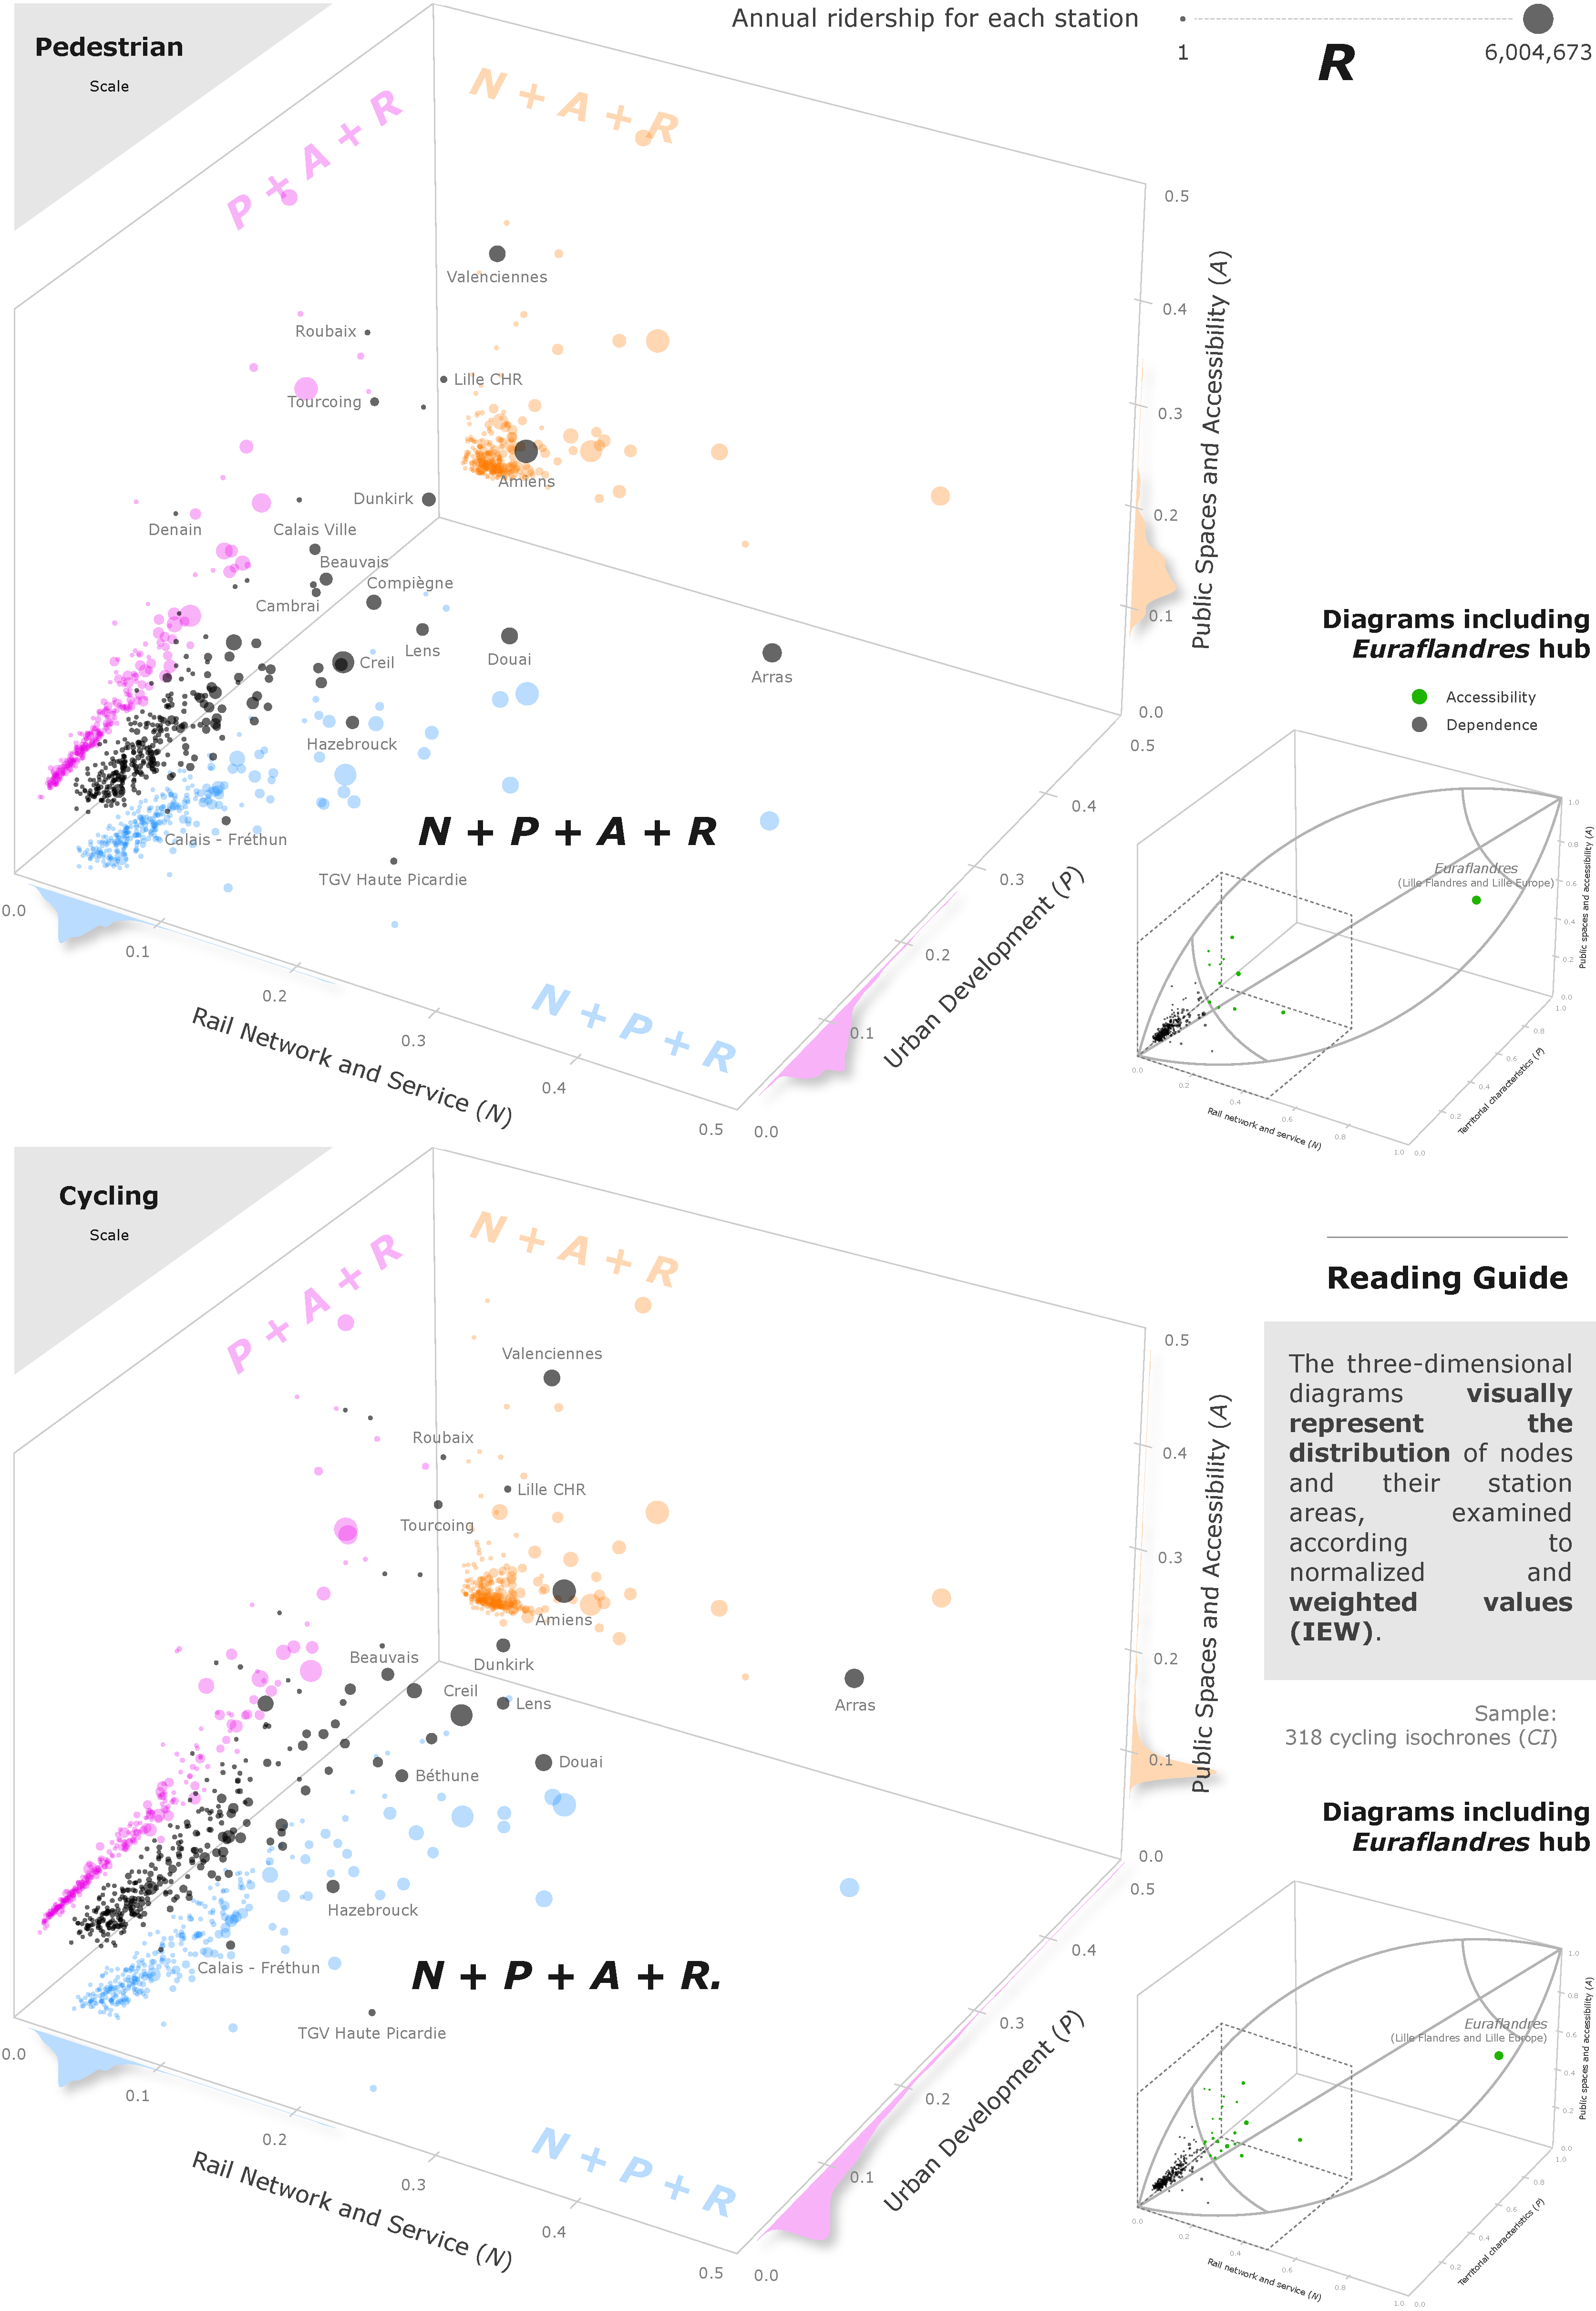
\includegraphics[width=1\columnwidth]{src/Figures/Chap-6/EN_NPART_Cubes.pdf}}
    \vspace{5pt}
    \begin{flushright}\scriptsize{
    Creation: \textcolor{blue}{Dylan Moinse (2024)}
    \\
    Authors: \acrshort{NPART} Research Project
    }\end{flushright}
\end{figure}

% Station positions - dependency
For all the geographical areas analyzed, the majority of the stations studied fall into the \Commas{dependent} category (see \hyperref[fig-chap6:diagramme-cubes]{Figure~\ref{fig-chap6:diagramme-cubes}}, page \pageref{fig-chap6:diagramme-cubes}). This is particularly true for both types of isochrones, where the proportion of stations considered \Commas{dependent} reaches 96.23\% for the pedestrian scale (\(PI\), 306 stations) and 92.77\% for the bicycle scale (\(CI\), 295 stations). It is worth noting that no train station neighborhood is in a state of profound \Commas{imbalance} favoring one of the three dimensions, nor in a state of \Commas{saturation}; however, the Euraflandres station neighborhood tends to approach this situation.%%Translated%%

% Station positions - accessibility (PI)
At both the pedestrian and bicycle scales, only a handful of nodes and station neighborhoods can be classified as \Commas{accessible} or \Commas{balanced,} using the terminology of \textcolor{blue}{Luca} \textcolor{blue}{\textcite[202]{bertolini_spatial_1999}}\index{Bertolini, Luca|pagebf}. More specifically, only 12 stations fall into this category for \(PI\), while 23 are classified as such for \(CI\). It appears that the 12 \Commas{accessible} stations for \(PI\) are also accessible for \(CI\). These include the stations in Amiens, Arras, Compiègne, Douai, Dunkirk, \textsl{Euraflandres}, Lens, Lille CHR, Pont de Bois, Roubaix, Tourcoing, and Valenciennes (see \hyperref[fig-chap6:diagramme-cubes]{Figure~\ref{fig-chap6:diagramme-cubes}}, page~\pageref{fig-chap6:diagramme-cubes}). As we can observe, the \Commas{accessible} stations at the pedestrian scale are either located in central municipalities of the \acrfull{MEL} or in the urban center of certain sub-prefectures of the region.%%Translated%%

% Station positions - accessibility (CI)
It is therefore worth noting that by expanding the station neighborhoods to adapt their size to the range of light individual mobility, the region sees its number of so-called \Commas{accessible} connection points double. The 11 stations that join this category due to the expansion of the stations' influence areas are as follows: Beauvais, Béthune, Boulogne-sur-Mer, Boulogne–Tintelleries, Calais Ville, Creil, Croix–Wasquehal, La Madeleine, Lille Porte de Douai, Saint-Quentin, and Saint-Roch (see \hyperref[fig-chap6:diagramme-cubes]{Figure~\ref{fig-chap6:diagramme-cubes}}, page~\pageref{fig-chap6:diagramme-cubes}). In this regard, the stations that become \Commas{accessible} as a result of the isochrone extension are either located in other sub-prefectures of the region or near the central stations of the main metropolitan areas.%%Translated%%

% Literature
The identification of a substantial majority of stations classified in the \Commas{dependent} category is hardly surprising at the regional level, given the diversity of the territories covered and the variety of rail services within the studied system. This result contrasts with observations in the literature, \textcolor{blue}{Freke} \textcolor{blue}{\textcite[46]{caset_planning_2019}}\index{Caset, Freke|pagebf} highlighting a predominance of \Commas{imbalanced} stations favoring the quality of the \acrfull{RER} service at the expense of design in the Brussels region. The finding of a higher proportion of stops with an imbalance against the location is supported by \textcolor{blue}{\textcite[190]{kutty_assessment_2018}}\index{Kutty, Najeeba Ali Kunju Abdulla|pagebf} and \textcolor{blue}{\textcite[19]{monajem_evaluation_2015}}\index{Monajem, Saeed|pagebf}\index{Ekram Nosratian, Farzan|pagebf}, who report this profile for 20\% of metro stations in Tehran, compared to only 5\% at the other extreme. Regarding the \acrfull{BRT} networks in Wates and Tehran, \textcolor{blue}{\textcite[15]{alfyan_node-place_2022}}\index{Alfyan, Muhammad Yusuf|pagebf}\index{Widyastuti, Dyah Titisari|pagebf} and \textcolor{blue}{\textcite[13]{pezeshknejad_evaluating_2020}}\index{Pezeshknejad, Parsa|pagebf}\index{Monajem, Saeed|pagebf}\index{Mozafari, Hamid|pagebf} also identify a majority of stops in asymmetric situations, the first study indicating an imbalance at the expense of urban development and the second at the expense of connections, particularly regarding walkability. In contrast, the main group of metro stations modeled by \textcolor{blue}{\textcite[12]{dou_integrating_2021}}\index{Dou, Mingxuan|pagebf}\index{Wang, Yandong|pagebf}\index{Dong, Shihai|pagebf} is in a state of \Commas{balance} in Shanghai, as is \textcolor{blue}{\textcite[197]{reusser_classifying_2008}}\index{Reusser, Dominik~E.|pagebf}\index{Loukopoulos, Peter|pagebf}\index{Stauffacher, Michael|pagebf}\index{Scholz, Roland~W.|pagebf} in the context of the Swiss rail network.%%Translated%%

% Transition
We have observed that the number of stations characterized by good coordination between the three dimensions addressed doubles when we expand the perimeter of the station neighborhoods, validating the hypothesis put forward by \textcolor{blue}{\textcite[518]{caset_measuring_2018}}\index{Caset, Freke|pagebf}\index{Vale, David~S.|pagebf}\index{Viana, Cláudia~M.|pagebf}, which suggests a marked contrast between rail service areas evaluated at 800 or 1,200 meters and those measured at 3,000 meters. This result implies that expanding the spatial scale allows for a better capture of local and regional dynamics that influence the \Commas{balance} between network, territory, and connectivity functions. More generally, we observe a widening gap between the least well-ranked stations and their surroundings and those that are at the forefront. This assessment raises questions about the specific factors that place these stations in such situations of \Commas{accessibility} or \Commas{dependency.} We will explore the determining components, ensuring to distinguish between pedestrian and bicycle ranges.%%Translated%%

% 6.4.2.2.
\needspace{1\baselineskip} % Reserve space
\subsubsection*{Profile of the \Commas{Accessible} and \Commas{Dependent} Stations based on Descriptive Indicators
    \label{chap6:results-profil-gares-dependance}
    }

% Statistical IEW values
On average, the values corresponding to the weighted indicators (\acrshort{IEW}) for stations classified as \Commas{accessible} (\(Acs\)) and \Commas{dependent} (\(Dpt\)) are as follows:
\begin{customitemize}
    \item Regarding the node (\(N\)), the average weighted value reaches 0.013 for \(N_{Acs}\) and 0.003 for \(N_{Dpt}\) for pedestrian and cycling scales. The gap in favor of the first category is thus 5.051 times greater for the pedestrian scale (\(PI\)), while it decreases to 3.646 for the cycling scale (\(CI\));
    \item As for the place (\(P\)), the average weighted value is 0.024 for \(P_{Acs}\) versus 0.006 for \(P_{Dpt}\) at the pedestrian scale. This gap in favor of accessible stations is 4.395 for \(PI\) and 3.641 for \(CI\);
    \item For the connections (\(A\)), the average weighted value is 0.025 for \(A_{Acs}\) and 0.007 for \(A_{Dpt}\) at the pedestrian scale. The gap is thus 3.518 for \(PI\) in favor of accessible stations, and decreases to 2.344 for \(CI\);
    \item Regarding the traffic (\(RT\)), the normalized average value is 0.151 for \(RT_{Acs}\) versus 0.006 for \(RT_{Dpt}\). The gap is thus 23.532 for \(PI\) and 18.345 for \(CI\), in favor of accessible stations.
\end{customitemize}%%Translated%%

% Differences in IEW values - statistics - in favor of accessible stations
In detail, in terms of intra-variable differences, the three indicators showing the greatest distinction between categories for the pedestrian scale (\(PI\)) are \(N_{1}\), with a difference of 82.691, followed by \(A_{7}\) with 74.375, and \(N_{2}\) with 73.921. For the cycling scale (\(CI\)), the most discriminative criteria remain \(N_{1}\), with a difference of 66.146, \(N_{2}\) with 58.96, and \(A_{6}\) with 40.591. Conversely, some indicators show a difference favoring the stations classified as \Commas{dependent.} For the pedestrian scale (\(PI\)), the relevant indicators are \(P_{13}\), with a difference of 0.443, \(A_{10}\) with 0.593, and \(P_{3}\) with 0.916. For the cycling scale (\(CI\)), we find \(P_{13}\) with a difference of 0.557 and \(A_{10}\) with 0.622, while \(P_{3}\) shows a difference of 1.977.%%Translated%%

% Summary
In other words, the nodes classified as \Commas{accessible} show significantly higher relative values regarding the frequency of \acrshort{HST}, regardless of the day of the week (\(N_{1}\) and \(N_{2}\)). Furthermore, for the pedestrian station area, they benefit from better urban rail public transport connections (\(A_{7}\)), while for the cycling station area, they display better links with \acrshort{PBS} services (\(A_{6}\)). Conversely, the nodes classified as \Commas{dependent} are characterized by higher median household income (\(P_{13}\)), less abundant car parking availability in the \gls{public space} (\(A_{10}\)), and a stronger residential specialization in their territories (\(P_{3}\)), regardless of the spatial scale considered. More broadly, the average difference in indicators is 12.101 for the pedestrian scale (\(PI\)) and 8.537 for the cycling scale (\(CI\)), suggesting that the cycling perimeter somewhat tempers the disparities between \Commas{accessible} and \Commas{dependent} stations.%%Translated%%

% Transition
By taking into account the different values specific to each criterion and dimension, we were able to position each of the stations studied within the conceptual zones defined by \textcolor{blue}{Luca} \textcolor{blue}{\textcite[344]{bertolini_nodes_1996}}\index{Bertolini, Luca|pagebf}. This positioning analysis also allowed us to compare the so-called \Commas{accessible} and \Commas{dependent} stations based on the pedestrian and cycling scales, thus offering an innovative perspective on this issue. The final sub-section, dedicated to the evaluation of public transport nodes, focuses not on the intrinsic values of each dimension but rather on the relationships between them.%%Translated%%

% 6.4.2.3.
\needspace{1\baselineskip} % Reserve space
\subsubsection*{Intensity and Direction of the Relationships between the Constituent Axes of the Model
    \label{chap6:results-correlation-dimensions}
    }

% Node - ridership correlation (PI and CI)
From the perspective of the four dimensions structuring the \acrshort{NPART}, it appears that some of them are closely interconnected. By calculating Pearson's correlation matrices for each pair of dimensions, we first highlighted a particularly significant positive association between the dimension related to the quality of the rail network (\(N\)) and the one related to mobility demand for each station (\(RT\)). In the overall dataset, the coefficient of determination \(R^2\) thus reaches 0.93 between the dimensions concerning the rail node and station ridership, regardless of the geographical areas considered (\(PI\) and \(CI\)). The associated \(t\)-test\footnote{~
    The \(t\)-test is a statistical method used to determine whether a correlation might be due to chance or not, in a context where there is no underlying true relationship or difference (null hypothesis). It should be noted that the power of the \(t\)-statistic is directly influenced by the sample size. This is why the number of observations must always be considered when interpreting the significance of a \(t\)-test.
} with a high value of 43.60 demonstrates that this correlation is statistically highly significant, with the probability that it is due to chance being virtually zero. However, it appears that this strong linear relationship between the \textsl{Transit} and \textsl{Ridership per Time} components is only true for the subgroup of stations classified as \Commas{accessible,} with a correlation coefficient of 0.96. In contrast, this coefficient drops to a moderate value of 0.53 when the analysis is limited to stations classified as \Commas{dependent.} This observation results from a segmentation effect, indicating that the relationship between \(N\) and \(RT\) depends on the intensity and degree of articulation of the specific values of each dimension, characterizing certain stations as \Commas{accessible} nodes. In this perspective, we also explored the relationships between the other dimensions.%%Translated%%

% Node - design correlation (PI and CI)
A second significant positive relationship is established between the node (\(N\)) and the design, materializing through the layout of public spaces and local connectivity (\(A\)). Pearson's correlation coefficient \(R^2\) reaches 0.75 for the pedestrian station area (\(PI\)) and 0.64 for the cycling station area (\(CI\)). Even more pronounced than in the first relationship studied, we observe a considerable gap between the stations classified as \Commas{accessible} and those classified as \Commas{dependent.} The former display high determination coefficients (\(R^2\) of 0.77 for \(PI\) and 0.71 for \(CI\)), while for the latter, the correlation is nearly nonexistent (\(R^2\) of 0.21 for \(PI\) and 0.02 for \(CI\)).%%Translated%%

% Place - design correlation (PI and CI)
A final significant positive linear relationship appears between the dimensions related to place (\(P\)) and design (\(A\)), as seen in \hyperref[fig-chap6:diagramme-cubes]{Figure~\ref{fig-chap6:diagramme-cubes}} (on page \pageref{fig-chap6:diagramme-cubes}). This association remains significant at both the pedestrian and cycling scales, with determination coefficients of 0.80 (t-test of 23.36) and 0.77 (t-test of 21.47), respectively. These results suggest that the intensification of human activities within a given area originates from or results in marked interdependencies with the quality of public spaces. Always distinguishing between stations classified as \Commas{accessible} and those classified as \Commas{dependent,} and contrary to the two previous relationships analyzed, we observe minor variations in the pedestrian influence area of the stations, with correlation coefficients \(R^2\) of 0.77 for the former and 0.72 for the latter. However, the gap is slightly more pronounced in the cycling station areas, where the \Commas{accessible} stations show a coefficient of 0.80, compared to 0.65 for the \Commas{dependent} stations.%%Translated%%

% Literature
The statistical regression analysis applied to the different dimensions studied reveals interesting interdependencies, particularly within the subsample of stations classified as \Commas{accessible.} These quantitative measures echo the work on the extended \acrshort{NPM} developed by \textcolor{blue}{\textcite[289]{vale_extended_2018}}\index{Vale, David~S.|pagebf}\index{Viana, Cláudia~M.|pagebf}\index{Pereira, Mauro|pagebf}, which, like our study, highlight a significant positive correlation between the dimensions related to \Commas{place} and \Commas{design.} Similarly, \textcolor{blue}{\textcite[10]{zhang_network_2019}}\index{Zhang, Yuerong|pagebf}\index{Marshall, Stephen|pagebf}\index{Manley, Ed.~J.|pagebf} also demonstrated the same important link, with an \(R^2\) of 0.81. They also found a relevant relationship between the \Commas{node} and the \Commas{place} (\(R^2\) of 0.70), further confirming the observation by \textcolor{blue}{\textcite[289]{vale_extended_2018}}\index{Vale, David~S.|pagebf}\index{Viana, Cláudia~M.|pagebf}\index{Pereira, Mauro|pagebf} of a moderate correlation between the \Commas{node} and \Commas{design,} at a level of 0.60. However, this last point differs from our empirical observations, which seem to indicate a strong correlation between \(N\) and \(A\), particularly at the pedestrian scale for the \Commas{accessible} stations \textcolor{blue}{\autocite[79]{papa_accessibility_2015}}\index{Papa, Enrica|pagebf}\index{Bertolini, Luca|pagebf}. Finally, the major positive relationship between \(N\) and \(RT\), especially during peak hours for the \Commas{accessible} stations, represents a novel contribution to the literature on the \acrshort{NPM}. However, this does not imply that a mere improvement in infrastructure and rail service would suffice to increase demand. The bilateral nature of the relationship similarly suggests that demand induces infrastructure improvements, which evolve to meet this growing demand.%%Translated%%

% Transition
By adopting a first approach based on the \Commas{accessibility} and \Commas{dependence} zones, we were able to qualify and assign specific values to each station studied. This empirical work highlighted that the vast majority of stations and station areas are positioned on the side of \Commas{dependent} nodes and places, with no stop on the network fundamentally considered as \Commas{imbalanced}. Furthermore, we examined the interactions between the four dimensions structuring our \acrshort{NPART} model through the lens of this typology. It emerges that the so-called \Commas{accessible} stations benefit from feedback effects between these four dimensions. However, as \textcolor{blue}{\textcite[4]{zhang_make_2023}}\index{Zhang, Mengyuan|pagebf}\index{Lee, Jinwoo Brian|pagebf} point out, \Commas{\textsl{the five categories of the original node-place model do not encompass all possible typologies of station areas and transit-oriented development (TOD) forms}}. While we were able to classify the stations and their immediate environment at both the pedestrian and cycling scales using these various values, our analysis continues by refining the classification of the stations studied in order to further fine-tune this typology.%%Translated%%

% 6.4.3.
\needspace{1\baselineskip} % Reserve space
\subsection{Classification of Nodal Points and their Pedestrian and Cycling Accessible Areas
    \label{chap6:results-classification-gares}
    }

% Introduction
While stations and their immediate surroundings play a central role in the interconnection of spaces at the regional scale, not all benefit from an equivalent positioning in terms of connectivity, human activity density, or the quality of developments. In this context, the aim of this modeling is to propose a classification of stations and their influence areas based on their respective performances. The goal is to go beyond a binary categorization (\Commas{accessible} or \Commas{dependent}) and develop a more nuanced typology of nodal points and surrounding areas, taking into account their ability to meet the principles of \acrshort{TOD} and \acrshort{M-TOD}. The ambition is not limited to a statistical classification; it also aims, within a framework of convergence between data science and geography, to contextualize and give meaning to these categories. As previously indicated, and given the diversity of typologies obtained according to the defined parameters, the section devoted to the presentation of results focuses on a case study. This case study relies on a specific profile: an analysis based on weighted indicators using the statistical \acrshort{IEW} method during morning peak hours (\(RT_{2}\)), employing the k-means clustering method applied to both the pedestrian (\(PI\)) and cycling (\(CI\)) scales.%%Translated%%

% 6.4.3.1.
\needspace{1\baselineskip} % Reserve space
\subsubsection*{Classification of the Regional Rail Network and Surrounding Areas
    \label{chap6:results-classification-gares-classes}
    }

% Classes
As detailed in the \hyperref[chap6:methodologie-statistiques-nombre-clusters]{methodological sub-section on determining the optimal number of classes~\ref{chap6:methodologie-statistiques-nombre-clusters}} (on page~\pageref{chap6:methodologie-statistiques-nombre-clusters}), the application of the method used resulted in the identification of three station classes. In the context of our case study, the classification of the 318 stations and station areas, for both the pedestrian scale (\(PI\)) and cycling scale (\(CI\)), leads to the identification of a first class (\(C1\)) grouping the most attractive stations, with a well-developed and well-designed urban environment; a second class (\(C2\)), including stations with developed infrastructure located in dynamic areas, but weakly oriented towards mobility hubs; and a final class (\(C3\)), consisting of stations that are less well-served and located in areas dominated by automobile use.%%Translated%%

% Figure class change
\begin{figure}[h!]\vspace*{4pt}
    \caption{Towards a doubling of the number of stations included in the first class.}
    \label{fig-chap6:cubes-classification}
    \centerline{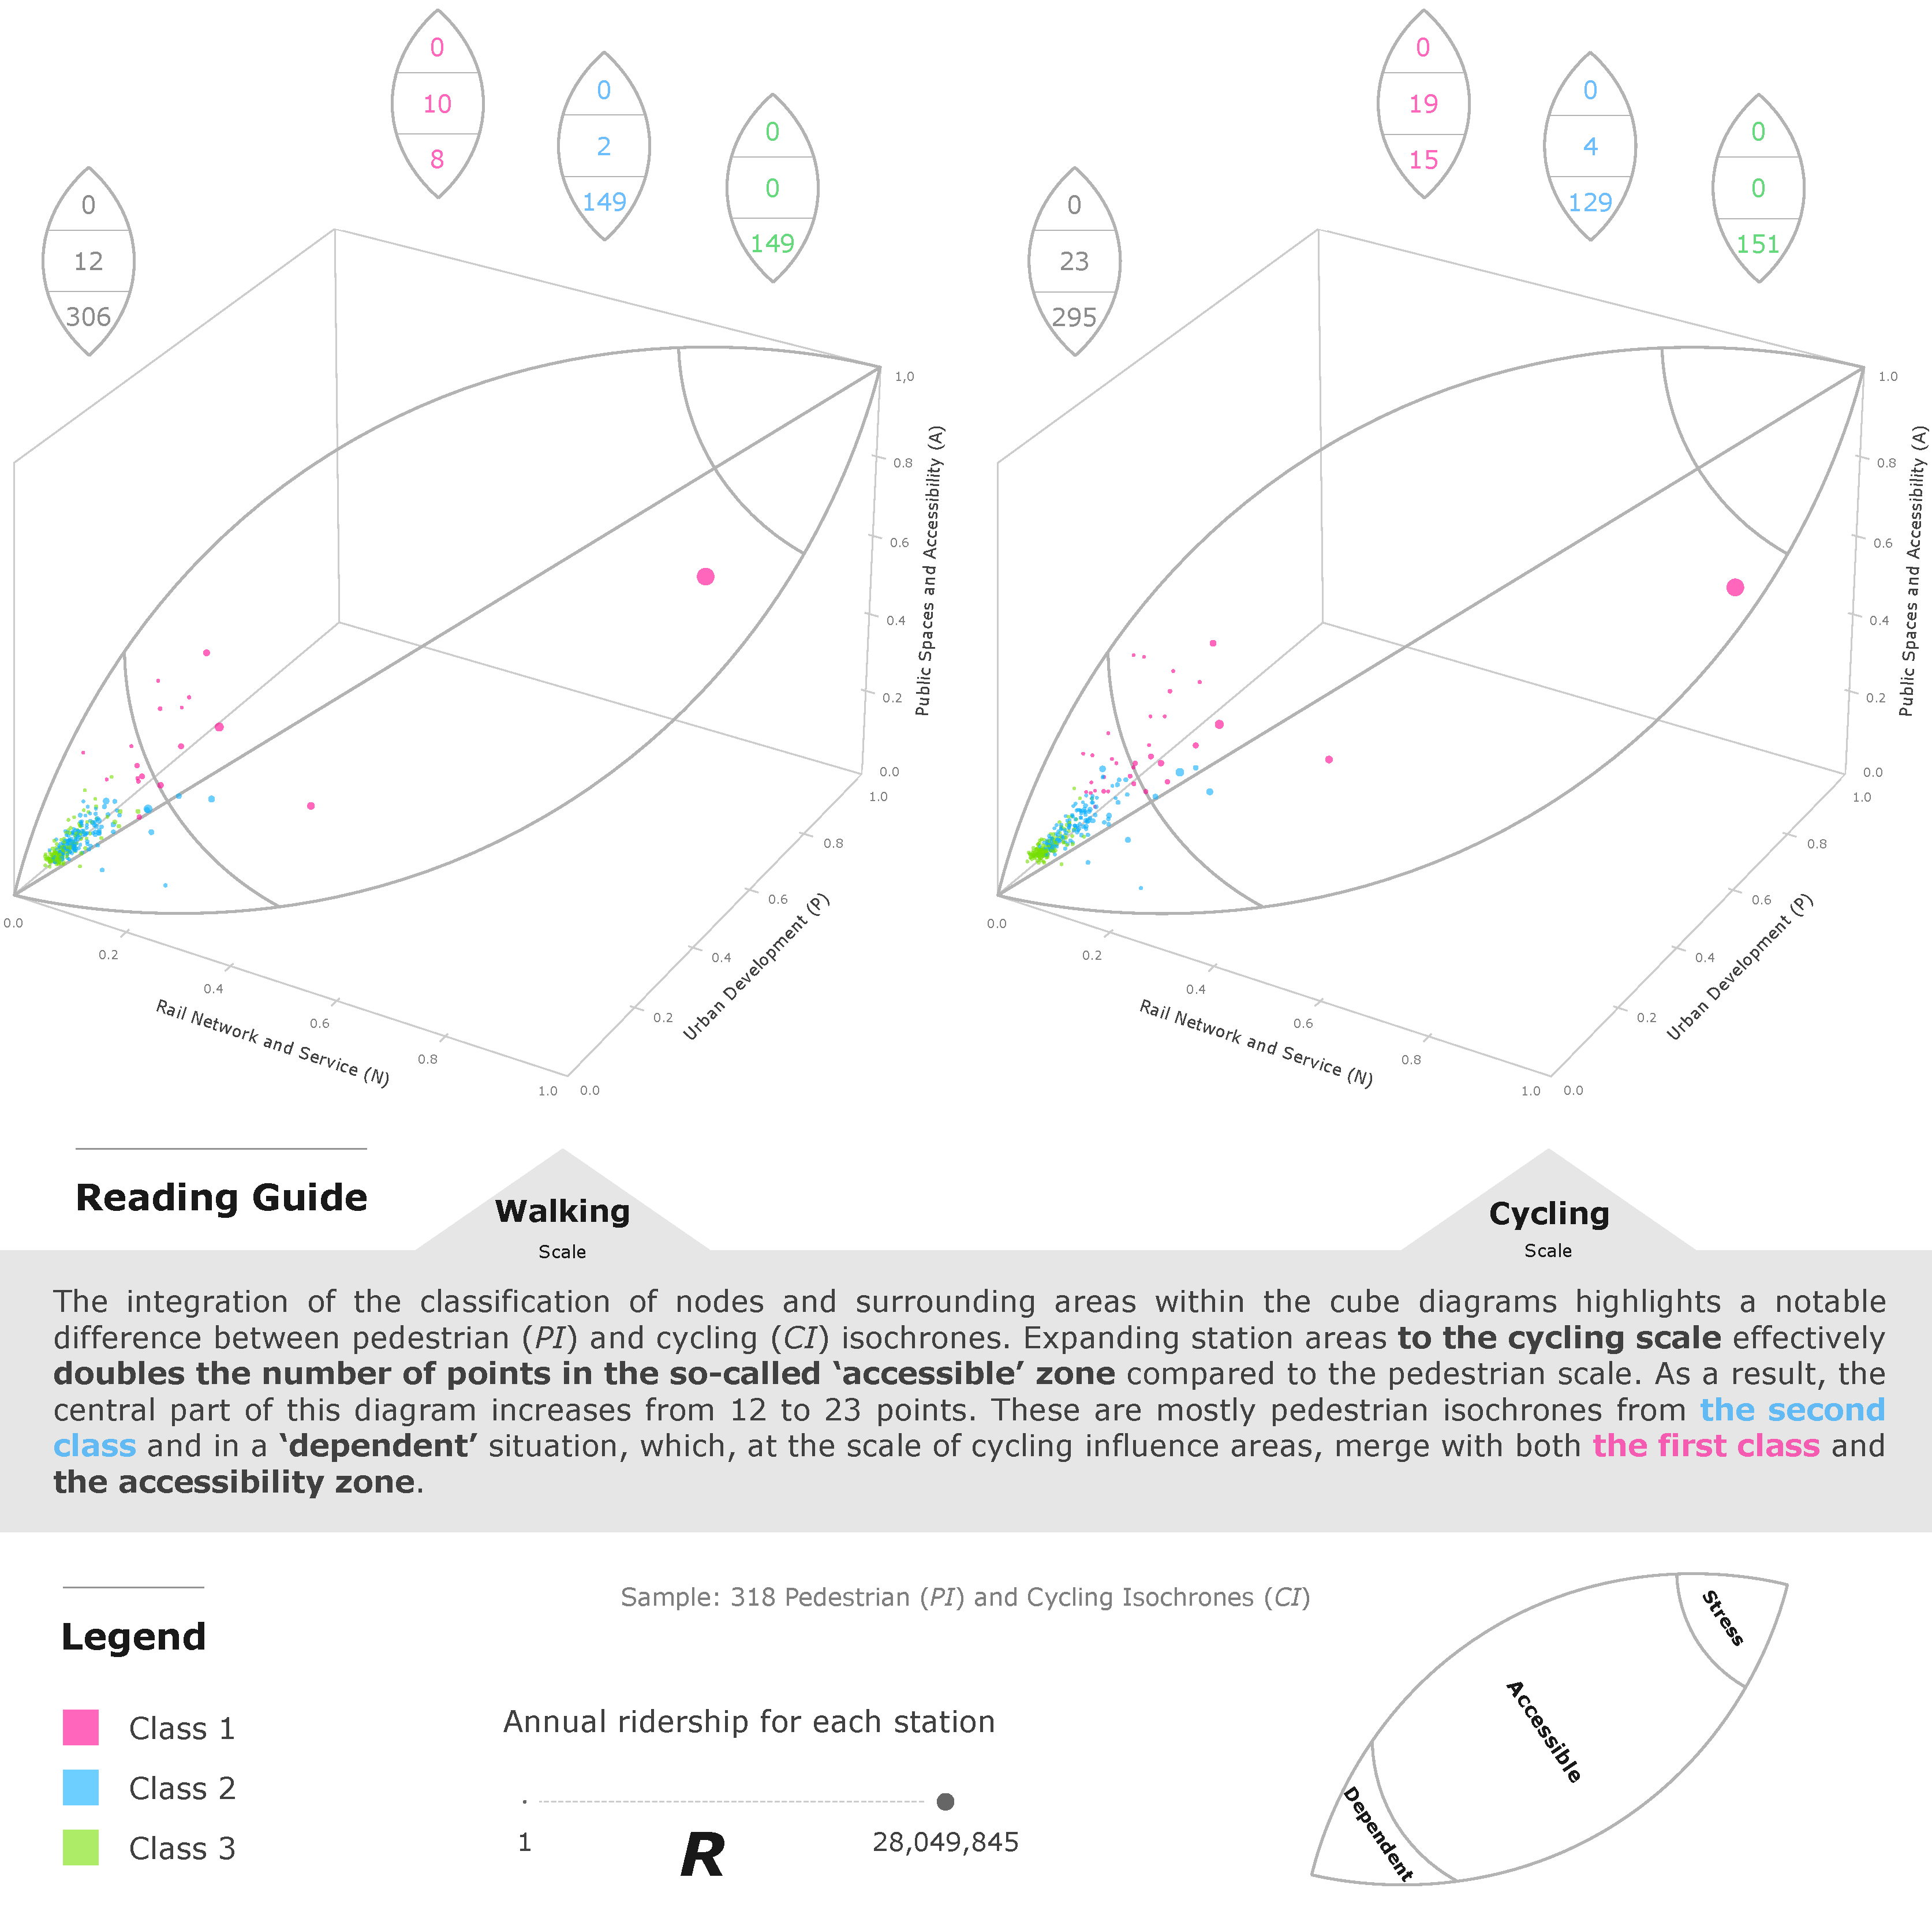
\includegraphics[width=1\columnwidth]{src/Figures/Chap-6/EN_NPART_Cubes_Classification.pdf}}
    \vspace{5pt}
    \begin{flushright}\scriptsize{
    Realization: \textcolor{blue}{Dylan Moinse (2024)}
    \\
    Authors: \acrshort{NPART} Research Project
    }\end{flushright}
\end{figure}

% PI vs CI Classes
As with the predominant proportion of stations classified as \Commas{dependent} in the region, almost all of these stations are also found in the last two classes. For \(PI\), only 5.66\% of stations are assigned to class \(C1\) (18 stations), while 47.48\% are in \(C2\) (151 stations) and 46.86\% in \(C3\) (149 stations). However, for \(CI\), the number of stations in \(C1\) doubles (10.69\%, 34 stations), mainly at the expense of \(C2\) (41.82\%, 133 stations), while \(C3\) maintains a similar share (47.48\%, or 151 stations). Thus, the expansion of station areas through light individual mobility allows various stops to move from class \(C2\) to \(C1\). It is worth noting that while expanding station areas does indeed double the number of stations in \(C1\), among the 16 new stations added to this category, 7 of them remain classified as \Commas{dependent} (see \hyperref[fig-chap6:cubes-classification]{Figure~\ref{fig-chap6:cubes-classification}}, on page~\pageref{fig-chap6:cubes-classification}).%%Translated%%

% Map Classification stations PI
\begin{carte}[h!]\vspace*{4pt}
    \caption{Distribution of stations in the regional rail network across the three classes of pedestrian-accessible station areas (\(PI\)).}
    \label{fig-chap6:classification-gares-pieton}
    \centerline{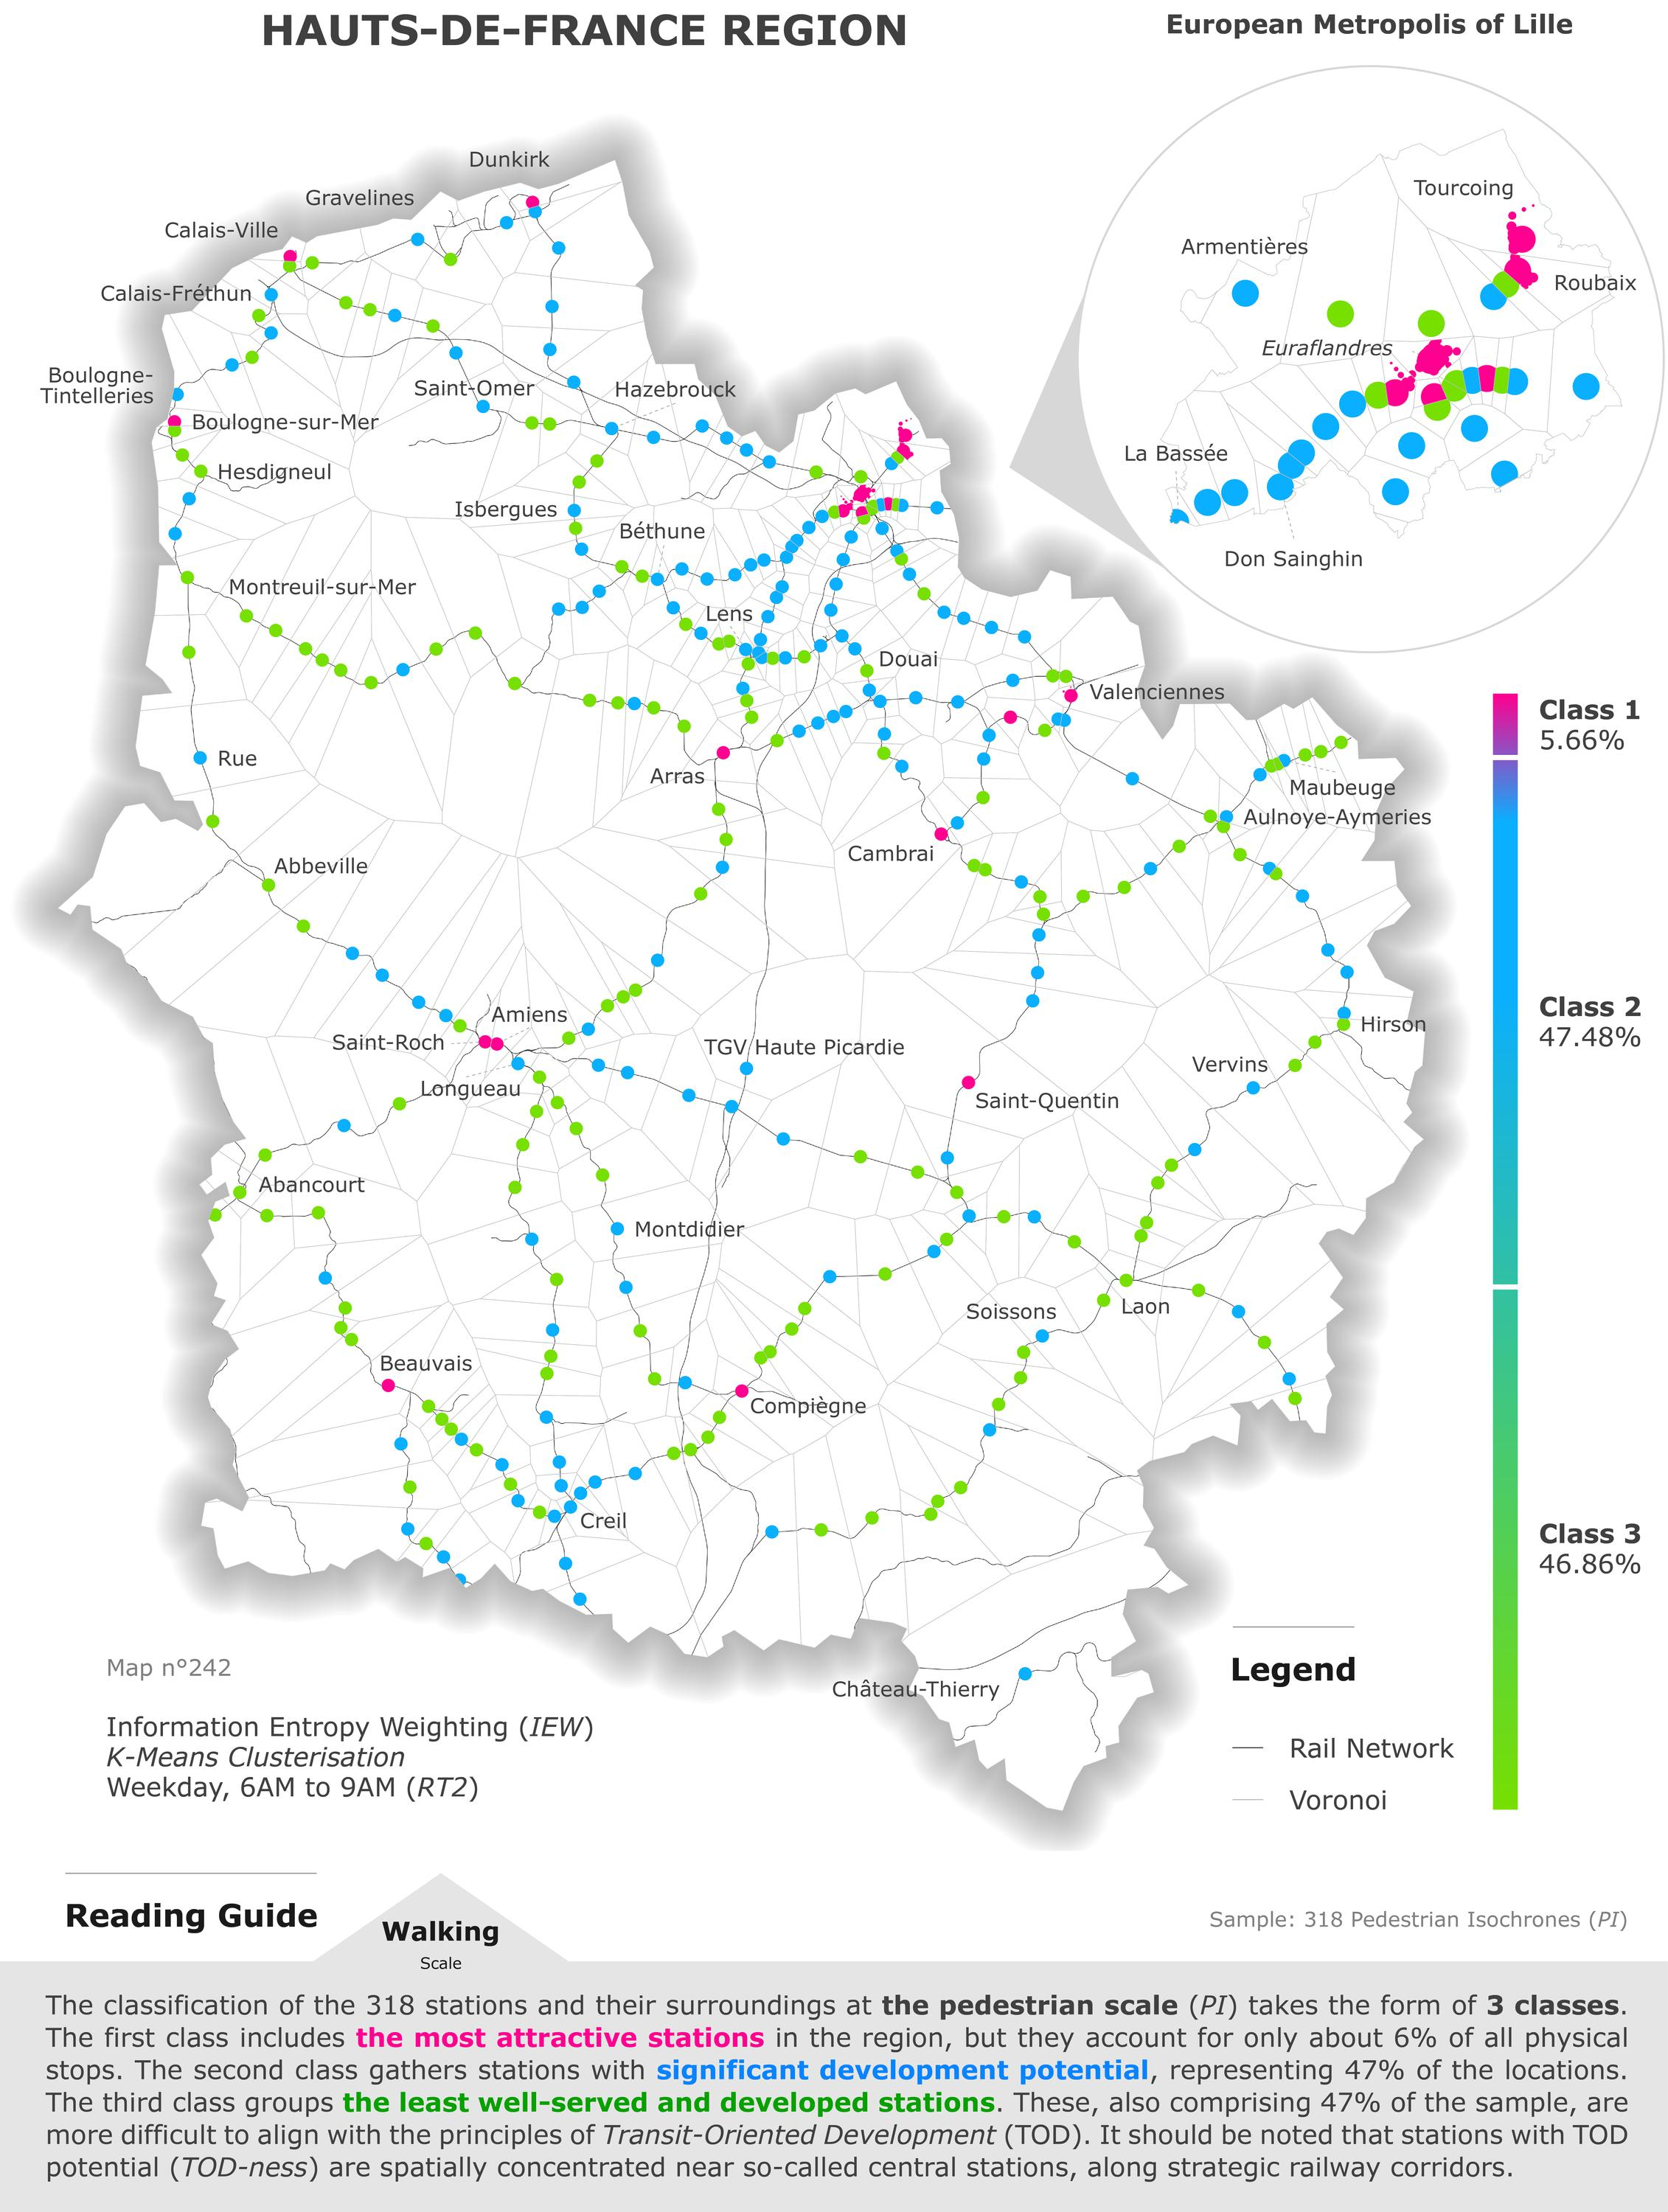
\includegraphics[width=1\columnwidth]{src/Figures/Chap-6/EN_NPART_Carte_Classification_PI.jpg}}
    \vspace{5pt}
    \begin{flushright}\scriptsize{
    Realization: \textcolor{blue}{Dylan Moinse (2024)}
    \\
    Authors: \acrshort{NPART} Research Project
    }\end{flushright}
\end{carte}

% Map Classification stations CI
\begin{carte}[h!]\vspace*{4pt}
    \caption{Distribution of stations in the regional rail network across the three classes of station areas accessible by light individual mobility (\(CI\)).}
    \label{fig-chap6:classification-gares-cyclable}
    \centerline{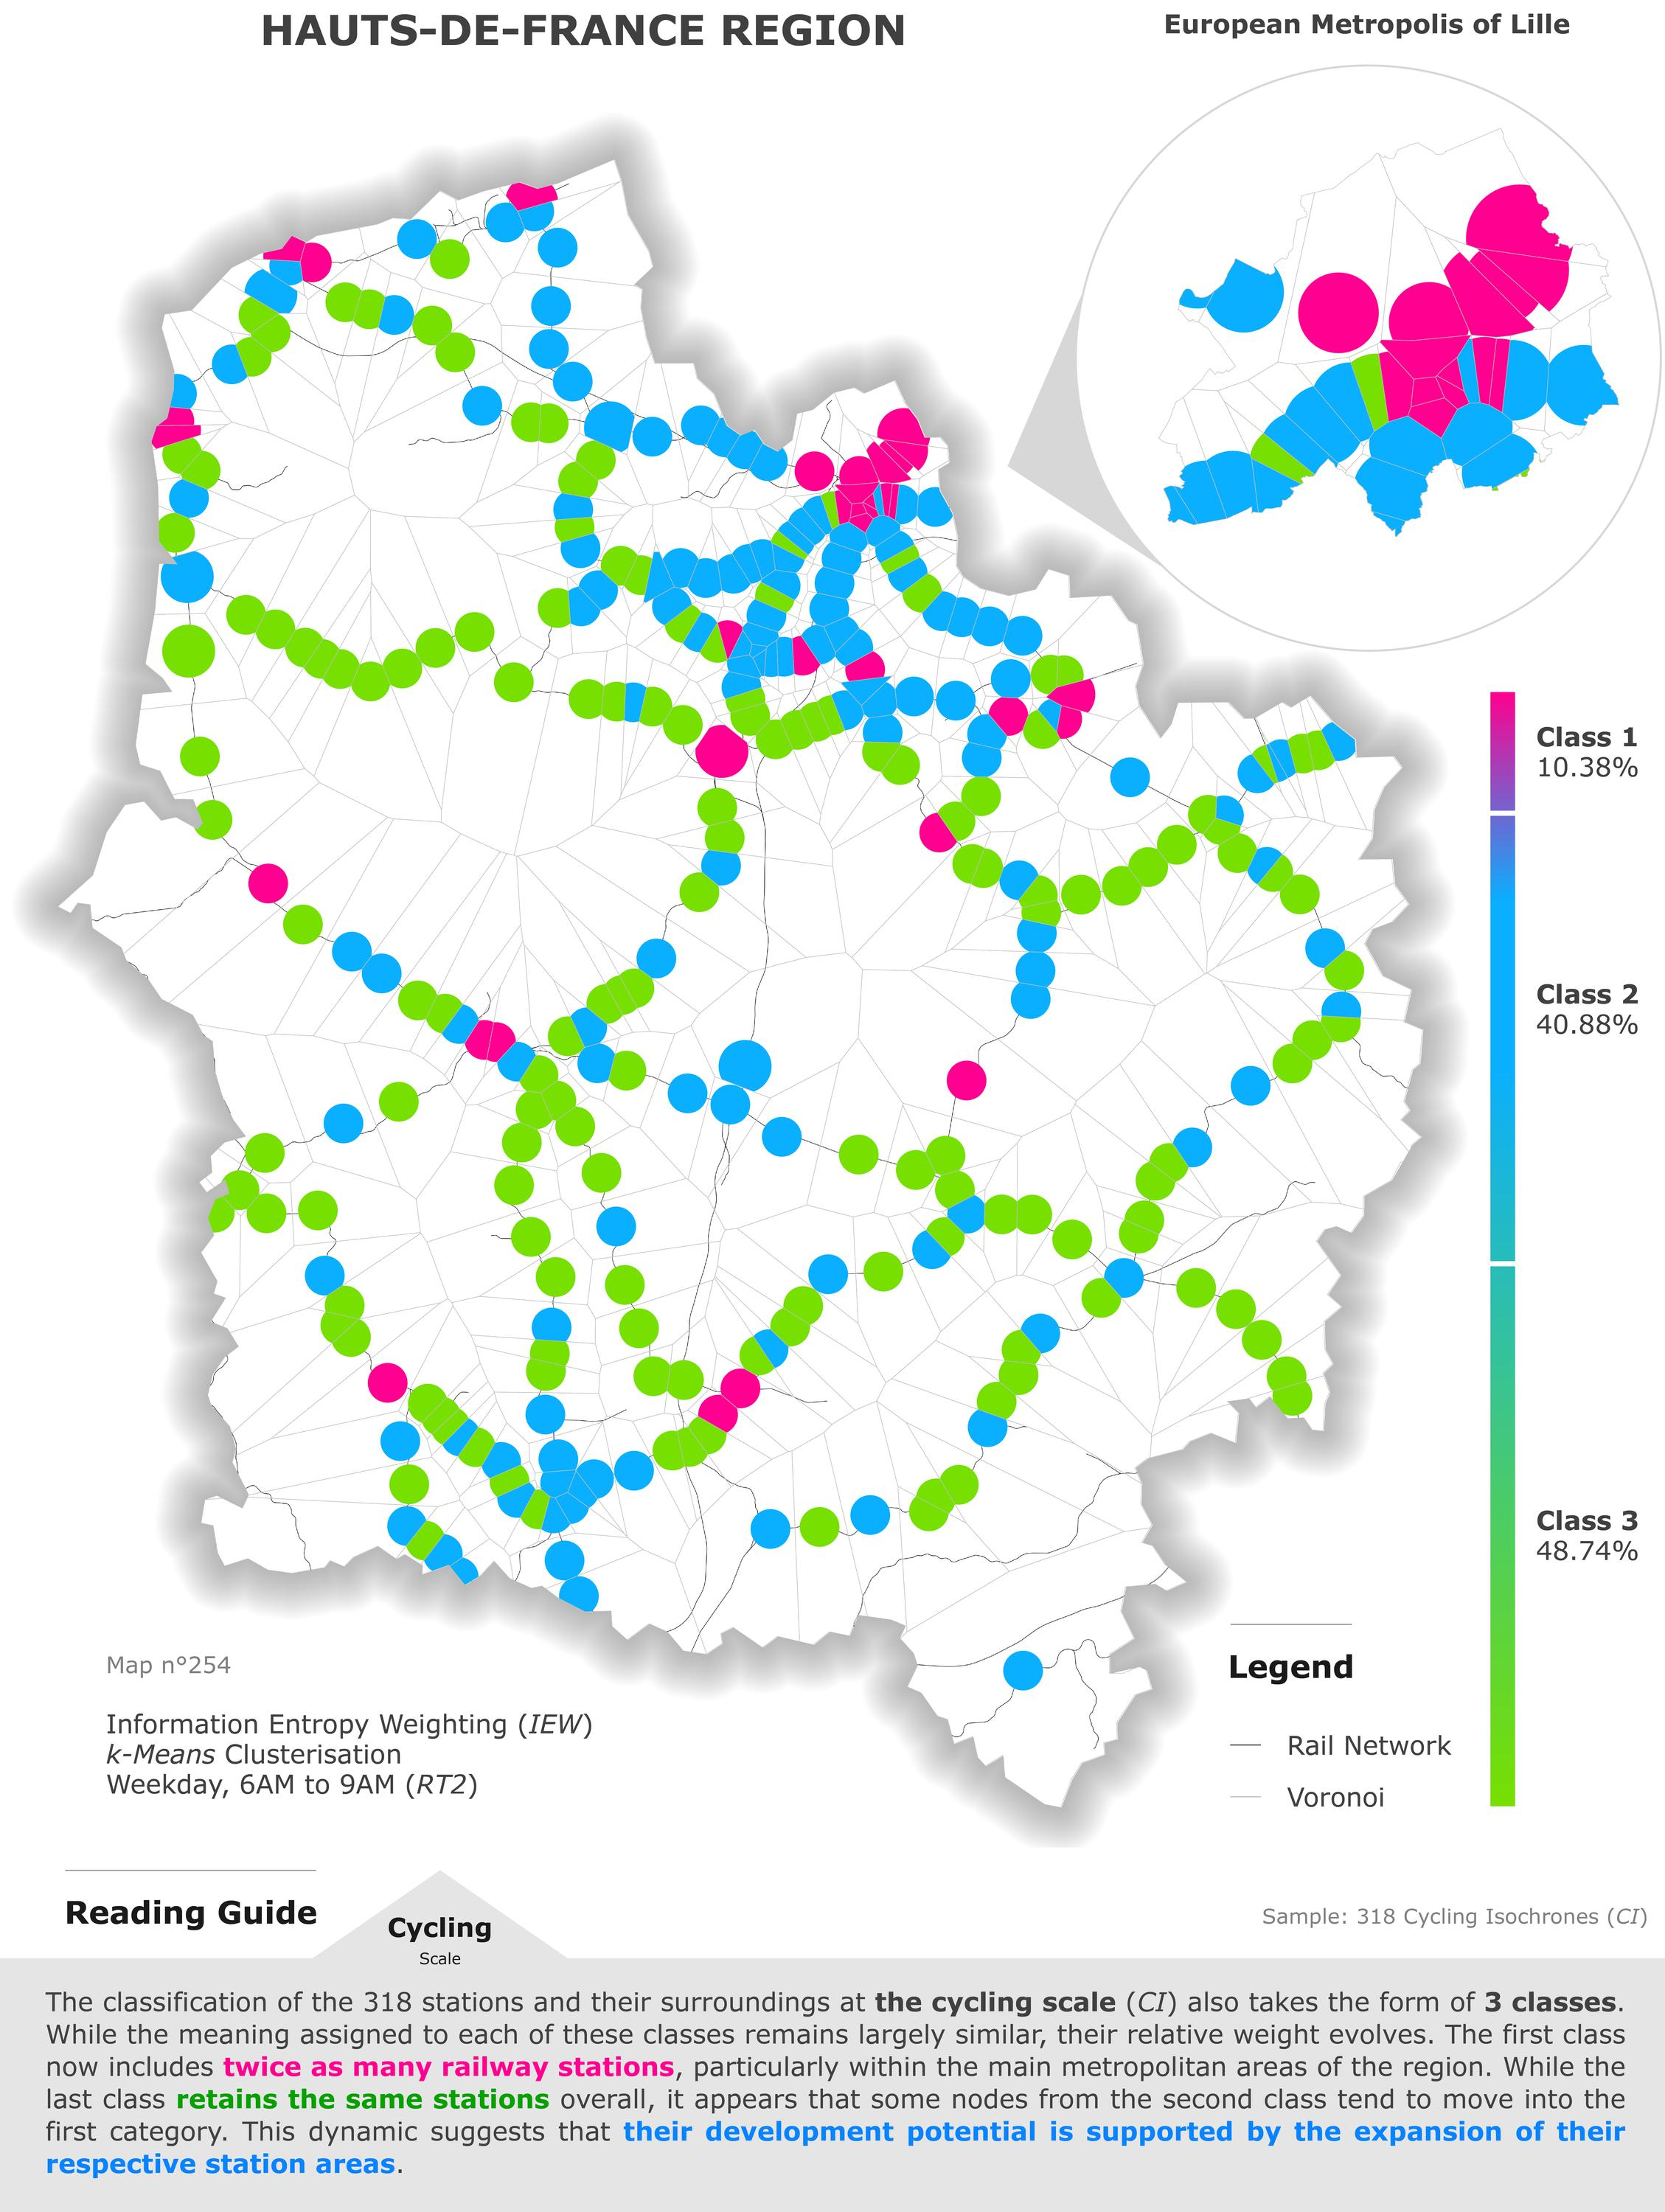
\includegraphics[width=1\columnwidth]{src/Figures/Chap-6/EN_NPART_Carte_Classification_CI.jpg}}
    \vspace{5pt}
    \begin{flushright}\scriptsize{
    Realization: \textcolor{blue}{Dylan Moinse (2024)}
    \\
    Authors: \acrshort{NPART} Research Project
    }\end{flushright}
\end{carte}

% Dependent accessibility typology VS classification
Thus, the classification approach allows us to deepen the characterization of stations and their surrounding areas, going beyond the simple dichotomy between \Commas{accessible} and \Commas{non-accessible} stations, particularly through the distinction that emerges between classes \(C2\) and \(C3\). It is also interesting to note that half of the stations classified in \(C1\), both for \(PI\) and \(CI\), are nonetheless positioned as \Commas{dependent}. Indeed, of the 18 and 34 stations classified in \(C1\) for \(PI\) and \(CI\) respectively, 8 and 15 of them correspond to stations in a \Commas{dependent} situation. This observation suggests that the typology based on the original \acrshort{NPM} model not only proves to be less precise but also diverges from the statistical classification performed. This finding aligns with contemporary critiques in the scientific literature, which encourage moving away from a simplistic interpretation based solely on a strictly diagrammatic view.%%Translated%%

% Station examples
From the perspective of pedestrian distances (\(PI\)), the 18 stations classified in \(C1\)\footnote{~
    Among these, 8 are located in the \Commas{dependent} zone, namely Beauvais, Boulogne~–~Tintelleries, Calais Ville, Cambrai, Denain, Lille Porte de Douai, Saint-Quentin, and Saint-Roch.
} include Amiens, Arras, Beauvais, Boulogne~–~Tintelleries, Calais Ville, Cambrai, Compiègne, Denain, Dunkerque, the \textsl{Euraflandres} hub, Lille CHR, Lille Porte de Douai, Pont de Bois, Roubaix, Saint-Quentin, Saint-Roch, Tourcoing, and Valenciennes. By comparing \hyperref[fig-chap6:classification-gares-pieton]{Map~\ref{fig-chap6:classification-gares-pieton}} (on page~\pageref{fig-chap6:classification-gares-pieton}) and \hyperref[fig-chap6:classification-gares-cyclable]{Map~\ref{fig-chap6:classification-gares-cyclable}} (on page~\pageref{fig-chap6:classification-gares-cyclable}), 16 additional stations are added to this list, exclusively based on the cycling area (\(CI\))\footnote{~
    These 16 stations are also considered \Commas{dependent} for both \(PI\) and \(CI\), except for Boulogne-sur-Mer, Croix~–~Wasquehal, and La Madeleine, which are classified in the \Commas{accessible} zone at the cycling scale.
}. These stations are: Abbeville, Annappes, Beau Marais, Boulogne-sur-Mer, Croix~–~Wasquehal, Croix l'Allumette, Hénin-Beaumont, Jaux, La Madeleine, Le Poirier Université, Lezennes, Loos-lez-Lille, Mont de Terre, Pérenchies, Pont de la Deûle, and Ronchin. Additionally, 10 stations move from \(C3\) to \(C2\) when we expand the station areas, namely Avion, Coron de Méricourt, Dreuil-lès-Amiens, Étaples~–~Le Touquet, Jeumont, Laon, Les Fontinettes, Louvroil, Thourotte, and Villers-Cotterêts.%%Translated%%

    % Tableau Classes par Ridership
% Table Classes by Ridership
%%Translated%%
    \begin{table}[h!]
    \centering
    \renewcommand{\arraystretch}{1.5}
    \resizebox{\columnwidth}{!}{
    \begin{tabular}{p{0.22\columnwidth}p{0.13\columnwidth}p{0.13\columnwidth}p{0.13\columnwidth}p{0.13\columnwidth}p{0.13\columnwidth}p{0.13\columnwidth}}
        %\hline
    \rule{0pt}{15pt} \small{\textbf{\textcolor{blue}{Classes}}} & \small{\textbf{\textcolor{blue}{\(RT_{1}\)}}} & \small{\textbf{\textcolor{blue}{\(RT_{2}\)}}} & \small{\textbf{\textcolor{blue}{\(RT_{3}\)}}} & \small{\textbf{\textcolor{blue}{\(RT_{4}\)}}} & \small{\textbf{\textcolor{blue}{\(RT_{5}\)}}} & \small{\textbf{\textcolor{blue}{\(RT_{6}\)}}}\\
        \hline
    \multicolumn{7}{l}{\textbf{Pedestrian Isochrones} (\(PI\))}\\
\multirow{2}{*}{\small{Class 1 (\(C1\))}} & \small{6.92\%} & \textbf{\small{5.66\%}} & \small{5.97\%} & \textbf{\small{5.97\%}} & \small{6.29\%} & \small{5.97\%}\\
& \small{22} & \textbf{\small{18}} & \small{19} & \textbf{\small{19}} & \small{20} & \small{19}\\
        \hdashline
\multirow{2}{*}{\small{Class 2 (\(C2\))}} & \small{30.19\%} & \textbf{\small{46.86\%}} & \small{45.91\%} & \textbf{\small{42.14\%}} & \small{37.11\%} & \small{33.65\%}\\
& \small{96} & \textbf{\small{149}} & \small{146} & \textbf{\small{134}} & \small{118} & \small{107}\\
        \hdashline
\multirow{2}{*}{\small{Class 3 (\(C3\))}} & \small{62.89\%} & \textbf{\small{47.48\%}} & \small{48.11\%} & \textbf{\small{51.89\%}} & \small{56.60\%} & \small{60.38\%}\\
& \small{200} & \textbf{\small{151}} & \small{153} & \textbf{\small{165}} & \small{180} & \small{192}\\
        \hline
    \multicolumn{7}{l}{\textbf{Cycling Isochrones} (\(CI\))}\\
\multirow{2}{*}{\small{Class 1 (\(C1\))}} & \small{11.32\%} & \textbf{\small{10.69\%}} & \small{11.01\%} & \textbf{\small{12.89\%}} & \small{5.97\%} & \small{6.29\%}\\
& \small{36} & \textbf{\small{34}} & \small{35} & \textbf{\small{41}} & \small{19} & \small{20}\\
        \hdashline
\multirow{2}{*}{\small{Class 2 (\(C2\))}} & \small{26.42\%} & \textbf{\small{41.82\%}} & \small{34.91\%} & \textbf{\small{36.16\%}} & \small{32.08\%} & \small{42.14\%}\\
& \small{84} & \textbf{\small{133}} & \small{111} & \textbf{\small{115}} & \small{102} & \small{134}\\
        \hdashline
\multirow{2}{*}{\small{Class 3 (\(C3\))}} & \small{62.26\%} & \textbf{\small{47.48\%}} & \small{54.09\%} & \textbf{\small{50.94\%}} & \small{61.95\%} & \small{51.57\%}\\
& \small{198} & \textbf{\small{151}} & \small{172} & \textbf{\small{162}} & \small{197} & \small{164}\\
        \hline
        \end{tabular}}
    \caption{Composition of the three classes of stations (\(C1\) to \(C3\)) based on the temporality and size of the station neighborhoods.}
    \label{table-chap6:classification-periodes}
        \vspace{5pt}
        \begin{flushleft}\scriptsize{
        \textcolor{blue}{Reading Guide:} On weekdays from 6:00 AM to 10:00 AM (\(RT_{2}\)), the first class \(C1\) includes 18 stations accessible by foot (\(PI\)), accounting for 5.66\% of the regional rail network. This proportion extends to 34 stations accessible by bicycle (\(CI\)), representing 10.69\% of the total sample.
        }\end{flushleft}
        \begin{flushright}\scriptsize{
        Realization: \textcolor{blue}{Dylan Moinse (2024)}
        \\
        Authors: \acrshort{NPART} Research Project
        }\end{flushright}
        \end{table}%%Rédigé%%

% Stations changing classes based on RT
Through a more dynamic analysis based on the temporal flow patterns, we observe a slight evolution in the classification. We thus examined the distribution of stations within the classes defined according to the \(RT_{2}\) reference (see \hyperref[table-chap6:classification-periodes]{Table~\ref{table-chap6:classification-periodes}}, on page~\pageref{table-chap6:classification-periodes}). It is interesting to note that, while the proportion of \(C1\) remains relatively stable around 6\% for the pedestrian scale (\(PI\)), it fluctuates between 6\% and 13\% at the cycling scale (\(CI\)). However, the class showing the most significant variation is undoubtedly \(C2\), particularly during the \(RT_{2}\) and \(RT_{4}\) periods, corresponding to morning peak hours and return hours, respectively. Indeed, the share of \(C2\) is higher during peak periods and for \(CI\), indicating increased attractiveness of stations in these spatio-temporal contexts. Thus, the temporal analysis of the classification reveals fluctuations in the composition of the classes according to periods, with a greater proportion of stations moving towards the \acrshort{TOD}-oriented classes when station areas are expanded and during peak times.%%Translated%%

% DNA Sequence Methodology
With the aim of obtaining a more systemic view of station classification shifts, we adopted the approach developed by \textcolor{blue}{\textcite[518]{caset_measuring_2018}}\index{Caset, Freke|pagebf}\index{Vale, David~S.|pagebf}\index{Viana, Cláudia~M.|pagebf}, which they called the \Commas{station DNA sequence}. This approach allows for representing the station's membership in clusters based on the variation in the size of their surrounding area. The \Commas{station DNA sequence} denoted as \(ADN\), relies on an ordered succession of classes to which each station is associated, based on the temporal scales (\(RT_{1}\) to \(RT_{6}\)) and geographical scales (\(PI\) and \(CI\)) considered (see \hyperref[equation:sequence-adn]{Formula~\ref{equation:sequence-adn}}, on page~\pageref{equation:sequence-adn}). For example, the \textsl{Euraflandres} hub exhibits a stable sequence, denoted as \Commas{\(C1C1C1C1C1C1-C1C1C1C1C1C1\)}, reflecting a consistency in its membership to \(C1\) across different spatio-temporal axes.%%Translated%%

% Station DNA Sequence Equation
\begin{equation}
\label{equation:sequence-adn}
\begin{aligned}
ADN_k = \sum_{k=1}^{6} \left( C^{RT_k}_{PI} + C^{RT_k}_{CI} \right)
\end{aligned}
\end{equation}
\begin{align*}
    &\text{where:} \\
    &ADN_i \text{ is the DNA sequence of station}~i\text{.}\\
\end{align*}%%Translated%%

% DNA Sequence Results
Finally, there are nearly as many combinations as stations observed, with no fewer than 263 unique sequences across the rail network for the 12 components analyzed. This result shows that only 1.89\% of the stations consistently retain the same class membership, a proportion that differs from the statistical analysis by \textcolor{blue}{\textcite[518]{caset_measuring_2018}}\index{Caset, Freke|pagebf}\index{Vale, David~S.|pagebf}\index{Viana, Cláudia~M.|pagebf}, where 49\% of Belgian stations are assigned to a constant typology, whether the radius is 0.7, 0.8, 1.2, or 3.0 kilometers. However, several recurring chains can be cited:
\begin{customitemize}
    \item \Commas{\(C2C2C2C2C2C2-C2C2C2C2C2C2\)}, representing stations entirely in \(C2\);
    \item \Commas{\(C2C2C2C2C2C2-C1C1C1C1C1C1\)}, corresponding to stations that transition from \(C2\) in the \(PI\) context to \(C1\) for \(CI\) across all periods;
    \item \Commas{\( C3C3C3C3C3C3-C2C2C2C2C2 \textcolor{blue}{C3} \)}, referring to stations that move from \(C3\) to \(C2\) across all time intervals except for the weekend.
\end{customitemize}%%Translated%%

% Transition
Continuing the exploration of the typology thus obtained, and after clarifying the distribution of stations within each category, we now undertake a detailed analysis of these classes. The following final sub-section provides a definition of the identified categories from a planning perspective, relying on a statistical analysis of the determining factors. This interpretative framework not only helps to grasp the specificities of each class, but also offers a conceptual reading of the observed distinctions, shedding light on the spatial and functional logics underlying this regional classification.%%Translated%%

    % 6.4.3.2.
    \needspace{1\baselineskip} % Reserve space
\subsubsection*{From the Definition to the Interpretation of the Established Categories
    \label{chap6:results-classification-gares-indicateurs}
    }

    % Methodology of Radars PI and CI and DNA sequence
In order to define the categories as accurately as possible based on statistical data, while providing a framework for operationalization and simplified communication, we chose to draw inspiration from the \Commas{butterfly model} as a visual reference framework for analysis. This conceptual representation was adopted to illustrate the \acrshort{NPM} in the doctoral thesis of \textcolor{blue}{Freke} \textcolor{blue}{\textcite[52]{caset_planning_2019}}\index{Caset, Freke|pagebf}, who applied it to the Belgian stations of Waterloo, Watermael, and Buggenhout, based on the initial models developed by the Province of \textcolor{blue}{\textcite{hollande-septentrionale_maak_nodate}}\index{Province de Hollande-Septentrionale@\textsl{Province de Hollande-Septentrionale}|pagebf}\index{Association Deltametropolis@\textsl{Association Deltametropolis}|pagebf}.%%Translated%%

    % Results of Radars PI and CI - general
Based on \hyperref[fig-chap6:radar-pi]{Figures~\ref{fig-chap6:radar-pi}} and \hyperref[fig-chap6:radar-ci]~\ref{fig-chap6:radar-ci} (pages~\pageref{fig-chap6:radar-pi} and~\pageref{fig-chap6:radar-ci}) divided into four axes constituting the \acrshort{NPART} model, we are able to compare not only the normalized and weighted values of each dimension and variable but also the two types of station districts. It appears that the dimensions related to station usage during morning peak hours (\(RT_{2}\)) and to the concentration and diversification of urban functions (\(P\)) generally show the lowest values. This statistical observation suggests that some stations compensate for low urban intensity with higher accessibility. In this specific case, the contribution of urban intensity to station usage is low in many cases, indicating potential for development through urban intensification. However, the lowest indicators are mostly found in the dimension related to local connectivity (\(A\)), particularly regarding metro and tram service (\(A_{7}\)), \acrshort{PBS} (\(A_{6}\)), bicycle parking availability (\(A_{5}\)), and the length of the cycling network (\(A_{4}\)), for both pedestrian (\(PI\)) and cycling (\(CI\)) areas, suggesting that soft connections remain largely marginalized.%%Translated%%

    % Radar PI Figure
    \begin{figure}[h!]\vspace*{4pt}
        \caption{Radar chart of the indicators of the model by station district class for pedestrian areas (\(PI\)).}
        \label{fig-chap6:radar-pi}
        \centerline{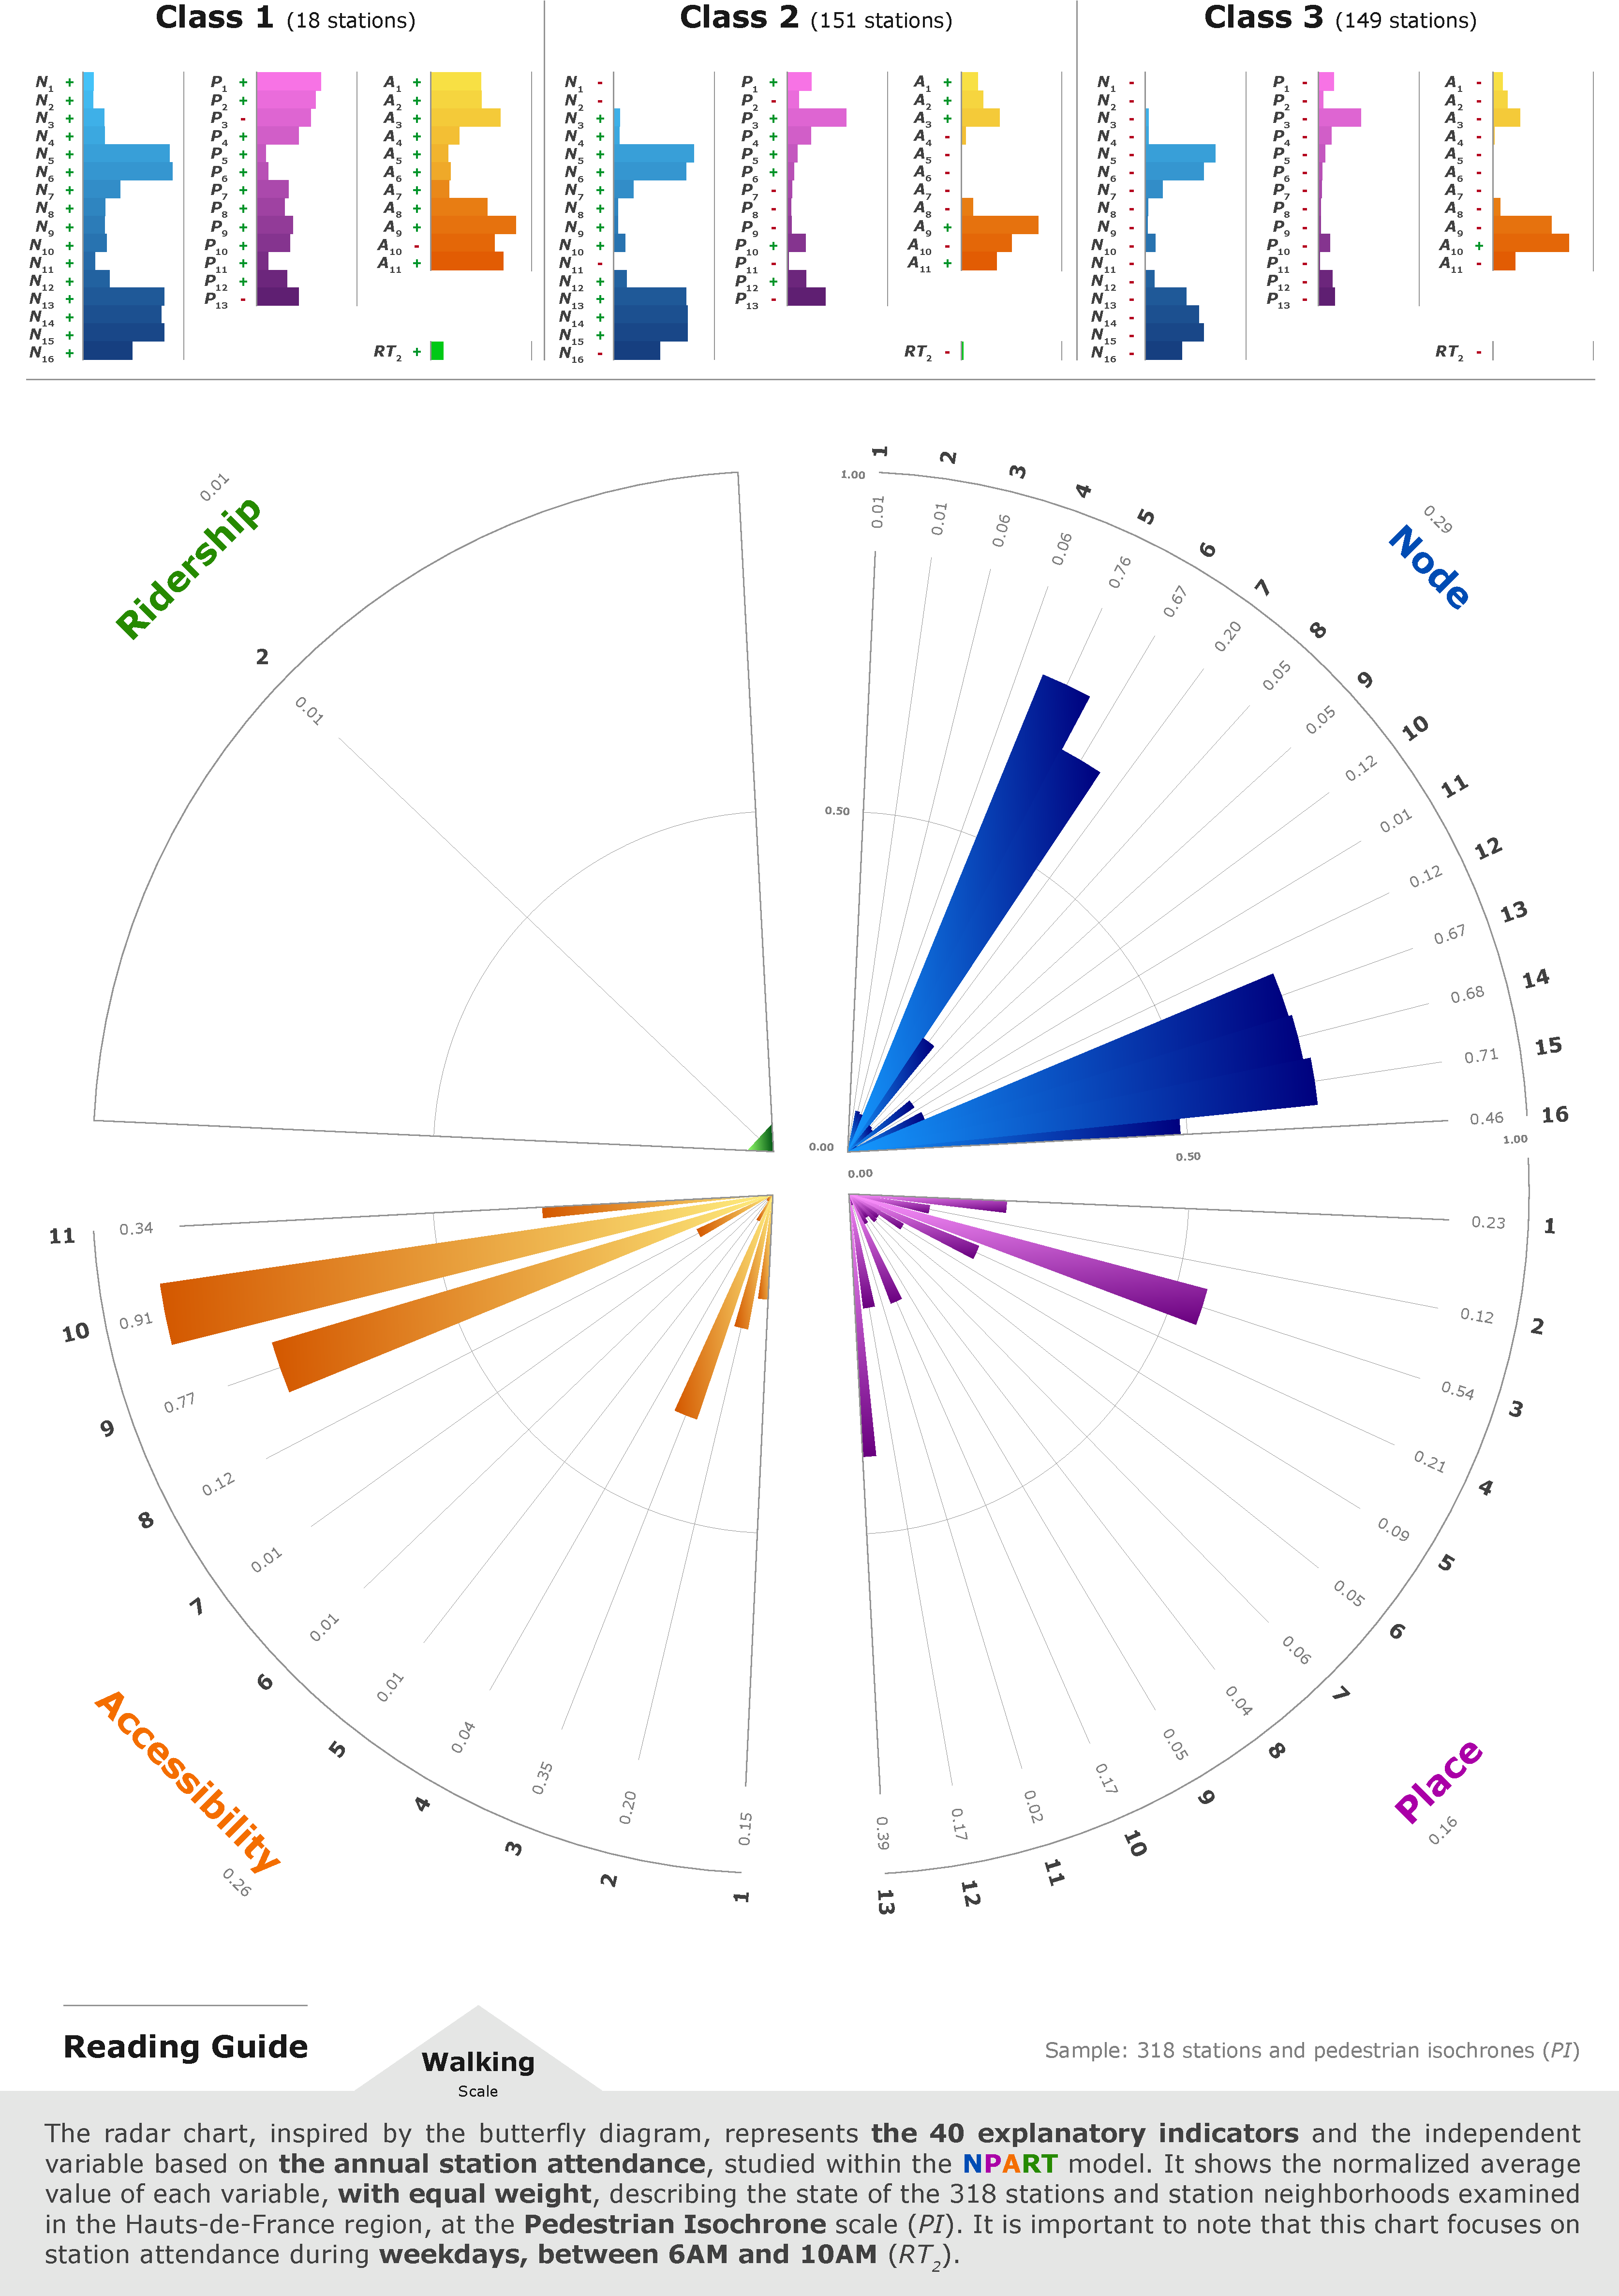
\includegraphics[width=1\columnwidth]{src/Figures/Chap-6/EN_NPART_Radar_PI.pdf}}
        \vspace{5pt}
        \begin{flushright}\scriptsize{
        Realization: \textcolor{blue}{Dylan Moinse (2024)}
        \\
        Authors: research project \acrshort{NPART}
        }\end{flushright}
    \end{figure}

    % Radar CI Figure
    \begin{figure}[h!]\vspace*{4pt}
        \caption{Radar chart of the indicators of the model by station district class for cycling areas (\(CI\)).}
        \label{fig-chap6:radar-ci}
        \centerline{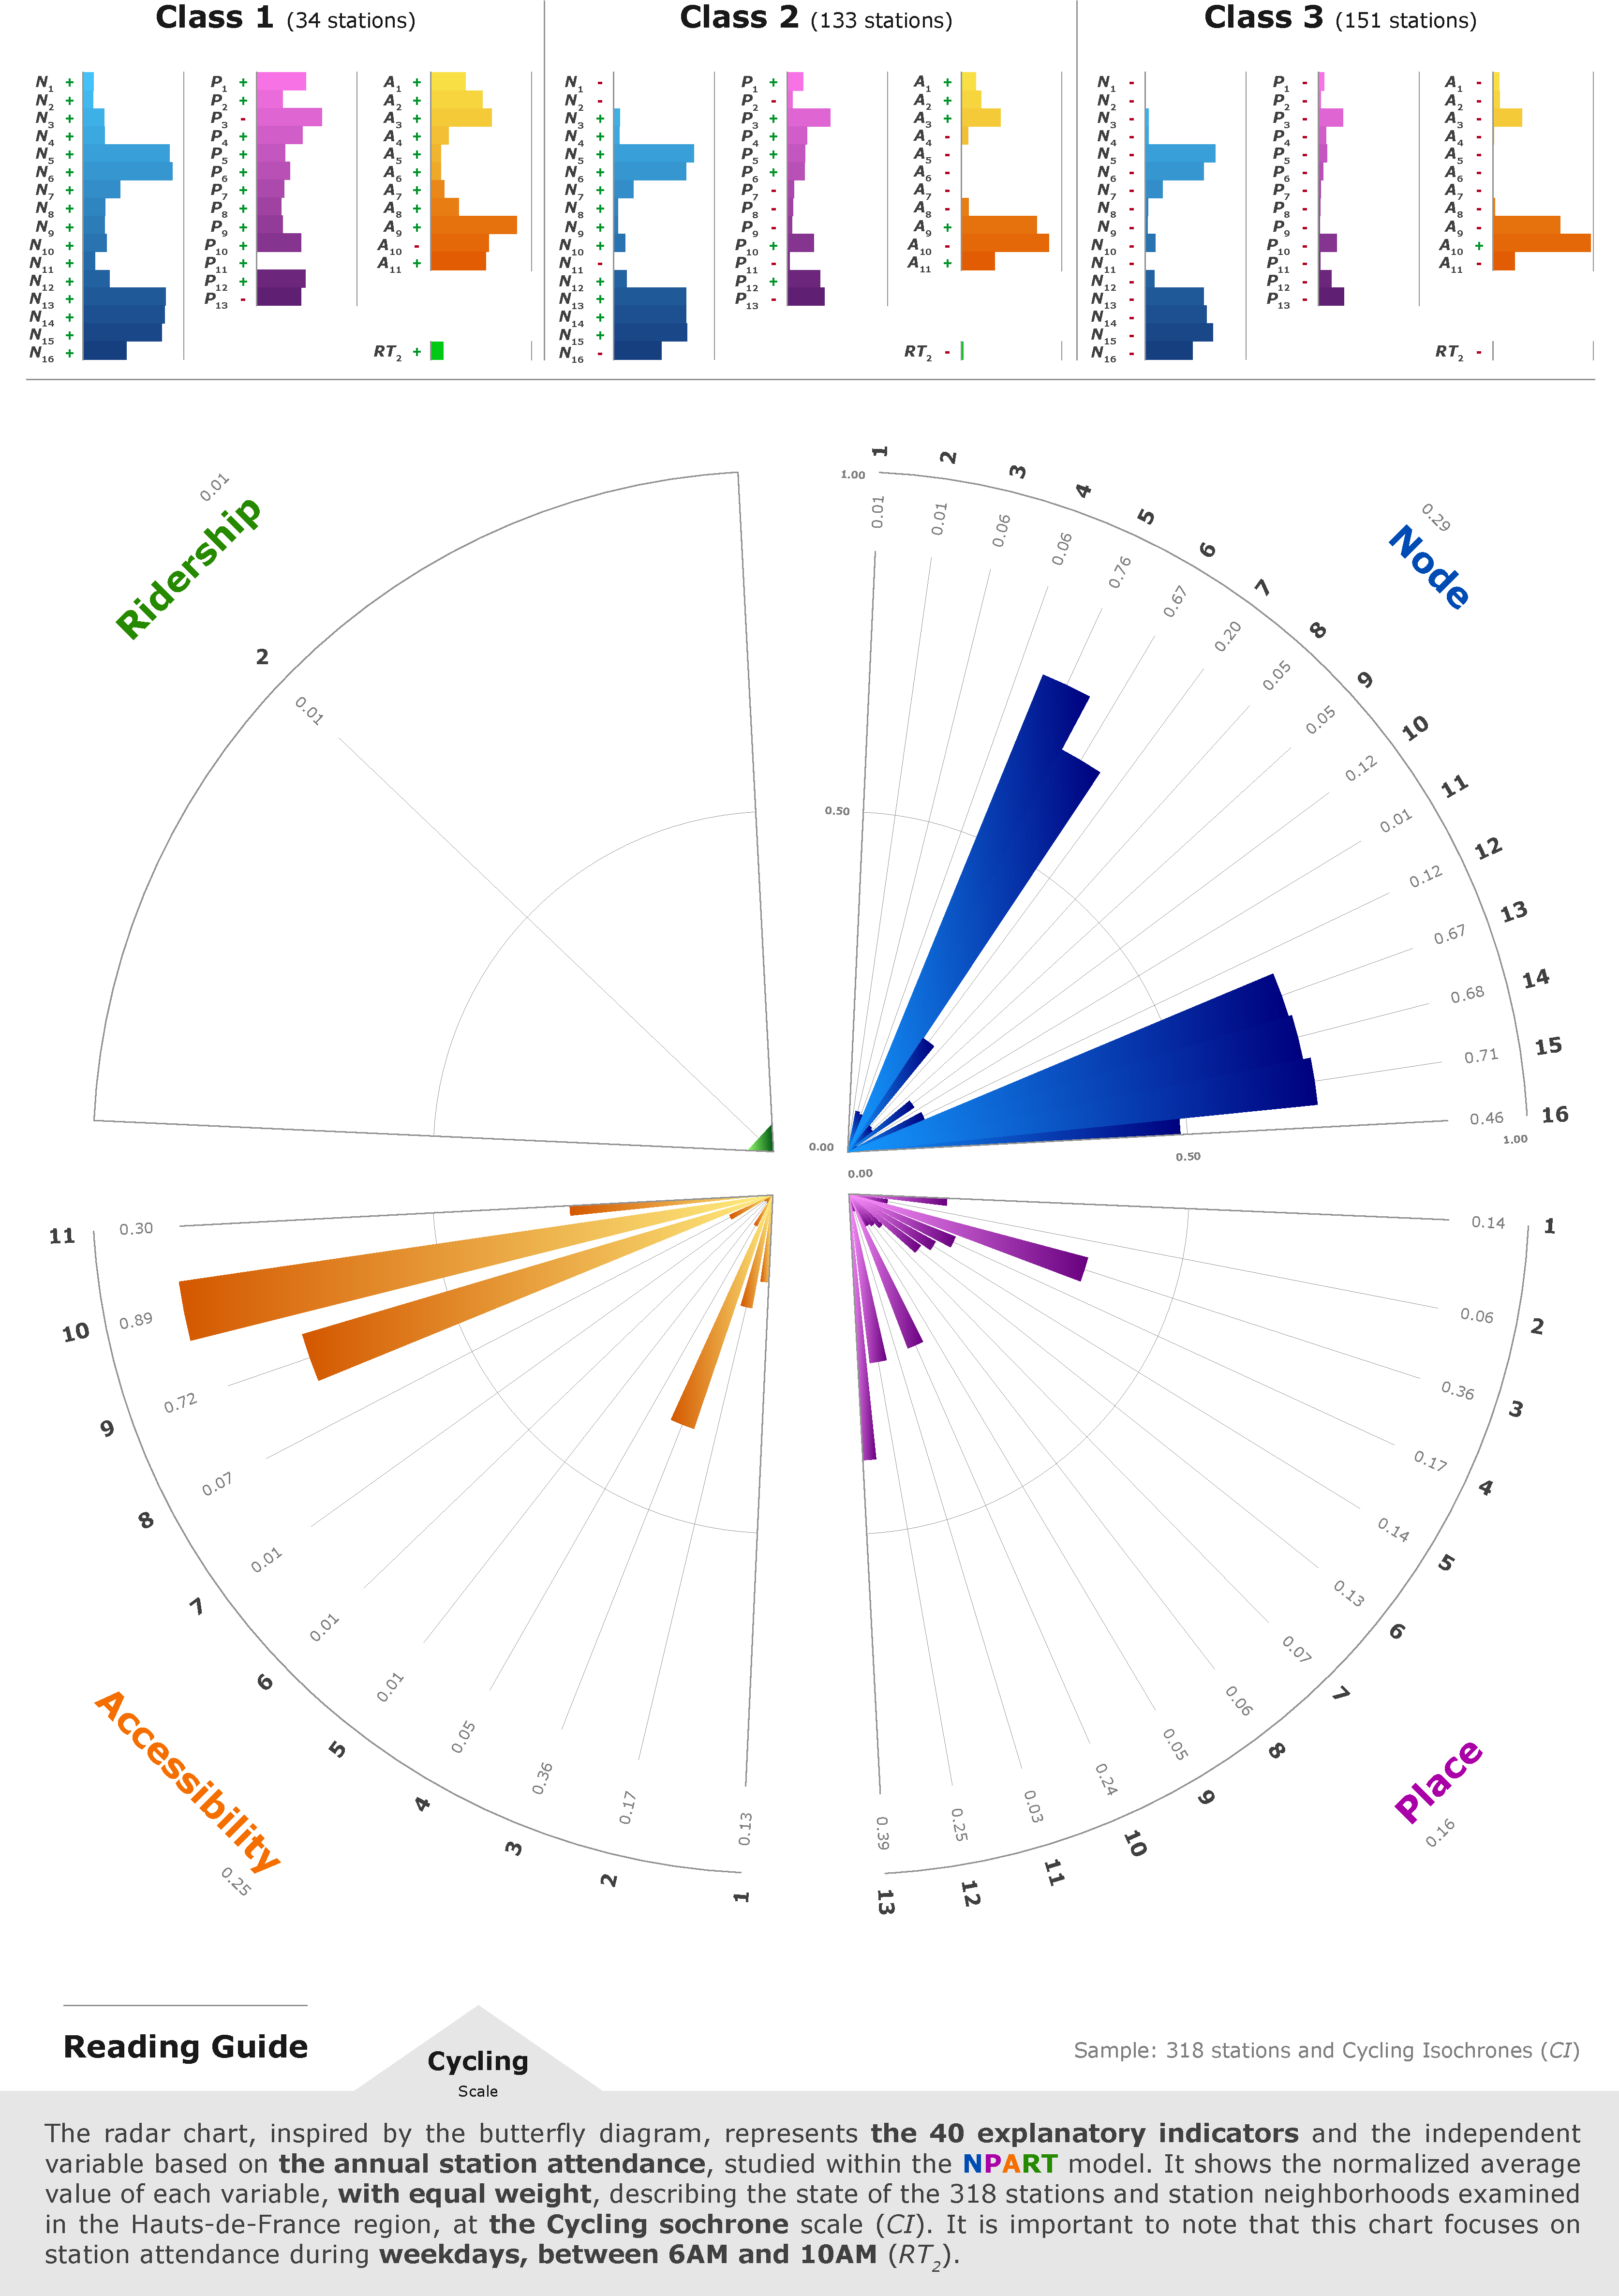
\includegraphics[width=1\columnwidth]{src/Figures/Chap-6/EN_NPART_Radar_CI.pdf}}
        \vspace{5pt}
        \begin{flushright}\scriptsize{
        Realization: \textcolor{blue}{Dylan Moinse (2024)}
        \\
        Authors: research project \acrshort{NPART}
        }\end{flushright}
    \end{figure}

    % Results of Radars PI and CI - difference
On average, the \acrshort{NPART} criteria show a 7\% gain between \(PI\) and \(CI\), across all dimensions. Excluding the dimensions \(N\) and \(RT\), where the geographic scale has no influence, the average growth reaches 12\%, suggesting that the extension of station districts tends to reduce disparities between the different areas covered by the railway network. Expanding the boundaries of station districts, it appears that 14 indicators see their relative value increase, particularly in the \(P\) dimension: the presence of green spaces (\(P_{6}\), +144\%), the property value of industrial activities (\(P_{11}\), +61\%), industrial and commercial specialization (\(P_{5}\), +59\%), the proportion of social housing (\(P_{12}\), +48\%), residential property value (\(P_{10}\), +41\%), the number of \acrshort{POIs} \Commas{intermediate} (\(P_{8}\), +35\%), \Commas{proximity} (\(P_{11}\), +20\%) and \Commas{superior} (\(P_{9}\), +7\%), as well as household income (\(P_{13}\), +1\%). Conversely, 10 indicators lose relative value, mainly in the \(A\) dimension: bus service (\(A_{8}\), -43\%), pedestrian network length (\(A_{1}\), -18\%), accessibility coefficient compared to the theoretical coverage rate (\(A_{2}\), -16\%), the rate of non-motorized households (\(A_{11}\), -11\%), motorized speed limits (\(A_{9}\), -6\%), and the restriction of car parking (\(A_{10}\), -3\%).%%Translated%%

    % Results of Radars PI and CI - classes
By filtering these values according to the station class affiliation, we are able to define each of the presented categories with greater precision (see \hyperref[fig-chap6:radar-pi]{radar Figures~\ref{fig-chap6:radar-pi}} and \hyperref[fig-chap6:radar-ci]~\ref{fig-chap6:radar-ci}, pages~\pageref{fig-chap6:radar-pi} and~\pageref{fig-chap6:radar-ci}):
\begin{customitemize}
    \item \(C1\) has the highest weighted average values for all dimensions, suggesting that this class performs the best and maintains a certain \Commas{balance} according to the measured parameters. For \(PI\), \(N\) reaches 0.42, \(P\) 0.35, \(A\) 0.47, and \(RT_{2}\) 0.10. For \(CI\), \(N\) is 0.36, \(P\) 0.35, \(A\) 0.38, and \(RT_{2}\) 0.06;
    \item \(C2\) shows values between \(C1\) and \(C3\). For \(PI\), \(N\) is 0.31, \(P\) 0.17, \(A\) 0.23, and \(RT_{2}\) 0.01. For \(CI\), \(N\) reaches 0.31, \(P\) 0.18, \(A\) 0.26, and \(RT_{2}\) 0.01;
    \item \(C3\) has the lowest values. For \(PI\), \(N\) is 0.22, \(P\) 0.12, \(A\) 0.20, and \(RT_{2}\) 0.00. For \(CI\), \(N\) is 0.25, \(P\) 0.10, \(A\) 0.21, and \(RT_{2}\) 0.00.
\end{customitemize}%%Translated%%

    % Interpretation of classes
In light of these data, we are able to give a more precise meaning to this classification within the regional framework of our empirical field. At this point, it is important to consider that class \(C1\) includes stations and their surrounding urban areas that are accessible on foot or by bike and adhere to or approach the planning principles of \acrshort{TOD} and \acrshort{M-TOD}. Class \(C2\), on the other hand, holds potential for \acrshort{TOD} development, under certain conditions that we will explain. Finally, class \(C3\) encompasses stations that are poorly served, relatively underdeveloped, and insufficiently equipped to support alternative mobility systems.%%Translated%%

    % Class C1
The first class, \(C1\), shows remarkably high scores in the four dimensions that make up the \acrshort{NPART}, positioning these stations as the closest candidates to the \acrshort{TOD} model and its variation, compared to what is present in the studied network. This class is primarily distinguished by better cycling connections within public spaces, a strategic position within the technical network, and strong industrial and commercial attractiveness. The most prominent criteria, characterizing this class by their value gaps with the other groups, are as follows:
\begin{customitemize}
    \item \textsl{Cycling infrastructure}\footnote{~
        Station districts \(C1\) are connected to an average fleet of 120 (\(PI\)) and 243 shared bikes (\(CI\)). The cycling network length is 670 (\(PI\)) and 1,378 kilometers (\(CI\)).
    }. \acrshort{PBS} services (\(A_{6}\)) are 42 and 191 times more numerous compared to \(C2\) and \(C3\) for \(PI\), and 58 and 1,014 times more for \(CI\). Additionally, the length of the cycling network (\(A_{5}\)) is 22 and 60 times (\(PI\)) and 14 and 126 times greater (\(CI\));
    \item \textsl{Urban rail public transport}\footnote{~
        Around 2 (\(PI\)) and 4 metro and tram stops (\(CI\)) serve the station districts \(C1\).
    }. The metro and tram service (\(A_{7}\)) is 89 times (\(PI\)) and 115 times (\(CI\)) higher compared to \(C2\), while \(C3\) does not benefit from such service;
    \item \textsl{High-speed system}\footnote{~
        On weekdays, 9 (\(PI\)) and 5 \acrshort{HST} (\(CI\)) trains serve the \(C1\) stations, compared to 8 and 4 \acrshort{HST} trains on weekends.
    }. The frequency of \acrshort{HST} trains is 19 and 91 times (\(PI\)) and 10 and 257 times higher (\(CI\)) on weekdays (\(N_{1}\)), and 19 and 113 times (\(PI\)) and 10 and 206 times higher (\(CI\)) on weekends (\(N_{2}\)) compared to other classes;
    \item \textsl{Rail network morphology}\footnote{~
        The centrality of intermediation for \(C1\) stations is 0.012 (\(PI\)) and 0.007 (\(CI\)).
    }. The centrality of intermediation (\(N_{11}\)) is 8 and 28 times (\(PI\)) and 4 and 20 times (\(CI\)) greater;
    \item \textsl{Estimated land use for industrial, commercial, and office purposes}\footnote{~
        Land for industrial, commercial, and office use is valued at 17,704 (\(PI\)) and~\euro7,033 per square meter (\(CI\)) within the station districts \(C1\).
    }. The property value of secondary and tertiary sectors (\(P_{11}\)) is 9 to 12 times (\(PI\)) and 4 to 6 times higher (\(CI\));
    \item \textsl{Flows}\footnote{~
        During morning peak hours, the \(C1\) stations are visited annually by more than 854,511 (\(PI\)) and 475,508 travelers (\(CI\)).
    }. Finally, station usage during morning peak hours (\(RT_{2}\)) is 8 and 57 times (\(PI\)) and 4 and 57 times higher (\(CI\)) than for \(C2\) and \(C3\).
\end{customitemize}%%Translated%%

    % Class C2 - part 1
While \(C1\) shows significantly higher weighted average values than \(C2\), with gaps of 103\% for \(P\) (\(PI\)) and 92\% (\(CI\)), 103\% for \(A\) (\(PI\)) and 50\% (\(CI\)), as well as 815\% for \(RT_{2}\) (\(PI\)) and 343\% (\(CI\)), the gap reduces for \(N\), reaching only 36\% (\(PI\)) and 16\% (\(CI\)). These discrepancies raise relevant questions regarding the identity of \(C2\). The main differences are observed in the treatment of public spaces:
\begin{customitemize}
    \item \textsl{Rather efficient rail network}\footnote{~
        \(C2\) stations are served by 38 (\(PI\)) and 41 \acrshort{TER} (\(CI\)) trains per weekday, compared to 15 and 17 \acrshort{TER} trains on weekends. On average, 16 hours and 14 hours (\(PI\) and \(CI\)) elapse between the departure of the first and last train, respectively during the week and weekend. In terms of inter-nodal accessibility, within a one-hour time budget, 2 other stations (\(PI\) and \(CI\)) are accessible from a \(C2\) station. To reach Euralille, one usually passes through 4 stations (\(PI\) and \(CI\)) in 62 minutes (\(PI\) and \(CI\)), compared to 6 stations (\(PI\) and \(CI\)) in 110 (\(PI\)) and 112 minutes (\(CI\)) to reach Châtelet.
    }. Regarding \(N\), the frequency of \acrshort{TER} lines (\(N_{3}\) and \(N_{4}\)) remains high with a small gap compared to the first class. The time range (\(N_{5}\) and \(N_{6}\)) is almost similar, as is the number of stations accessible within an hour (\(N_{12}\)) and the accessibility to major urban hubs (\(N_{13}\), \(N_{14}\), \(N_{15}\), and \(N_{16}\));
    \item \textsl{Residential attractiveness and low activity density}\footnote{~
        \(C2\) station districts are home to 3,085 (\(PI\)) and 1,473 inhabitants per square kilometer (\(CI\)), compared to 398 (\(PI\)) and 175 jobs per square kilometer (\(CI\)). 8\% (\(PI\)) and 6\% (\(CI\)) of the influence areas of \(C2\) are occupied by commercial activities. We count 44 (\(PI\)) and 116 \acrshort{POIs} of \Commas{proximity} (\(CI\)), 22 and 56 of \Commas{intermediate} range, and 7 and 20 of \Commas{superior} type.
    }. In \(P\), the population density (\(P_{1}\)) shows little variation, unlike job density (\(P_{2}\)) and commercial land use (\(P_{4}\)), with a notable gap observed for \acrshort{POIs} (\(P_{7}\), \(P_{8}\), and \(P_{9}\));
    \item \textsl{Fragmentation of connections between networks and territories}\footnote{~
        \(C2\) station districts are connected to an average fleet of 0 (\(PI\)) and 4 shared bikes (\(CI\)). The cycling network is 29 (\(PI\)) and 64 kilometers (\(CI\)) long, compared to 47 and 113 kilometers for the pedestrian network. The area of car parking spaces is 43,209 (\(PI\)) and 185,040 square meters (\(CI\)).
    }. The most significant differences come from the \(A\) dimension, where cycling infrastructure and services are notably insufficient (\(A_{4}\) and \(A_{5}\)), while the pedestrian network is relatively well-equipped (\(A_{1}\)). Moreover, the availability of car parking (\(A_{10}\)) is much more abundant, particularly at the cycling scale.
\end{customitemize}%%Translated%%

    % Class 2 - part 2
Class \(C2\) is distinguished by overall urban development levels and local connectivity about twice as low as those of the first category, while still maintaining a relatively high level of service. This allows us to infer that \(C2\) includes stations with potential for rail-oriented urban development, as the infrastructure and rail services are of good quality, although gaps remain in terms of human activity concentration and territorial hospitality. Furthermore, these are \acrshort{TOD} station districts with a residential predominance.%%Translated%%

    % Class 3
Finally, class \(C3\) records very low scores for all the indicators of the \acrshort{NPART}. The quality of rail service (\(N\)) is generally not ensured\footnote{~
    The frequency of \acrshort{TER} trains is 16 (\(PI\)) and 14 daily services (\(CI\)) on weekdays, and 7 and 6 daily services on weekends. With an average commercial speed of 64 (\(PI\)) and 63 kilometers per hour (\(CI\)). Only 2 directions (\(PI\) and \(CI\)) are offered from \(C3\) stations, allowing access to only one station within less than an hour (\(PI\) and \(CI\)).
}, with low \acrshort{TER} frequency, reduced commercial speed, and a poorly strategic position in the network, offering few directional choices and limited access to other stations within a given distance-time. The surrounding territories are underdeveloped or poorly planned (\(P\))\footnote{~
    The job density in \(C3\) station districts is 244 (\(PI\)) and 55 jobs per square kilometer (\(CI\)). Only 1\% (\(PI\)) and 0\% (\(CI\)) of the areas are dedicated to green spaces. Concerning \acrshort{POIs} in each area, the \Commas{proximity} range includes 25 (\(PI\)) and 33 (\(CI\)), the \Commas{intermediate} range includes 11 (\(PI\)) and 12 (\(CI\)), and the \Commas{superior} range includes 3 (\(PI\) and \(CI\)). The property value of industrial and commercial land is~\euro1,403 (\(PI\)) and~\euro1,220 per square meter (\(PI\)). In contrast, the median household income in these catchment areas is~\euro4,227 (\(PI\)) and~\euro4,383 per month (\(CI\)).
}, showing very low job density, relatively few green spaces, a very limited number of \acrshort{POIs}, and low property attractiveness for industrial and commercial sectors. These areas also host generally more affluent populations. In addition to the need for urban intensification, these station districts do little to encourage the use of the walking, light individual mobility, and public transport triad (\(A\))\footnote{~
    The total length of cycling facilities in each \(C3\) station district is 0 (\(PI\)) and 1 kilometer (\(CI\)), with 11 (\(PI\)) and 7 bicycle parking spaces (\(CI\)), and 3 (\(PI\)) and 0 \acrshort{PBS} (\(CI\)). We count 6 (\(PI\)) and 9 bus stops (\(CI\)). Meanwhile, the legal maximum car speed is 48 (\(PI\)) and 60 kilometers per hour (\(CI\)) and is accompanied by 19,740 (\(PI\)) and 36,894 square meters (\(CI\)) of car parking area. 86\% (\(PI\)) and 87\% of households (\(CI\)) in these catchment areas are motorized. Finally, the \(C3\) stations see an annual passenger flow of 14,858 (\(PI\)) and 8,308 (\(CI\)) during morning peak hours.
}, with almost nonexistent cycling infrastructure for both \(PI\) and \(CI\), and very limited bus service. Additionally, the space allocated to automobiles is generous, with moderate restrictions for motorized traffic and a high motorization rate among residents. Finally, this lack of accessibility and development results in very low station attendance (\(RT_{2}\)). In a way, class \(C3\) does not refer to \Commas{stations to close,} but rather stations with potential, where it would be worthwhile to explore development avenues combining \(N\), \(P\), and \(A\) in relevant and realistic combinations, to strengthen their attendance and trigger the \acrshort{TOD} spiral. This brings us to remind that the concept of planning is primarily a metropolitan and regional \Commas{string of pearls,} where each element in the system, from the largest to the smallest, has a role to play. Thus, the smallest stations should likely not be overlooked.%%Translated%%

    % Naming of classes and literature
The detailed analysis of each station leads us to summarize them, in a synthetic way, according to the classification requirements, as follows: \(C1\) includes nodes and areas truly oriented towards rail or those tending towards this model of planning, \(C2\) concerns nodes and areas with \acrshort{TOD} potential—some of which may also fall under \acrshort{TAD} \textcolor{blue}{\autocite[3]{renne_transit-adjacent_2009}}\index{Renne, John Luciano|pagebf}—and \(C3\) corresponds to self-centered nodes and areas, which tend to turn their back on transport infrastructure. This distinction between \acrshort{TOD}, \acrshort{TAD}, and self-centered systems aligns with the clustering produced, within the framework of \acrshort{NPM}, by \textcolor{blue}{\textcite[271]{li_transit_2019}}\index{Li, Zekun|pagebf}\index{Han, Zixuan|pagebf}\index{Xin, Jing|pagebf}\index{Luo, Xin|pagebf}\index{Su, Shiliang|pagebf}\index{Weng, Min|pagebf}, who identified a category falling under \acrshort{TAD}. This type of territorial configuration assumes spatial coherence between transport-related dimensions and land use, but without a fully achieved morphological and functional interconnection \textcolor{blue}{\autocite[47]{el_hadeuf_ville_2017}}\index{El Hadeuf, Mounya|pagebf}\index{Laterrasse, Jean|pagebf}.%%Translated%%

    % Meaning of classes
By extending the statistical analysis of the classes to extract trends and specifically examining the actual presence of \acrshort{TAD} within these groupings, it became necessary to go beyond the simple typology contrasting \acrshort{TOD}, \acrshort{TAD}, and non-\acrshort{TOD}. Based on a commonly accepted definition of \acrshort{TAD}, characterized by a high level of public transport service, high population density, and, conversely, relatively low station usage and density of pedestrian and cycling spaces, we identified 86 pedestrian station districts (\(PI\)) and 33 cycling station districts (\(CI\)), distributed across all the classes. To establish this classification, we selected stations and their associated local accessibility perimeters, considering that the quality of the public transport network (\(N\)) and population density (\(P_1\)) should be at least three times higher than station usage (\(RT\)) and local connectivity (\(A\)). A differentiated distribution of \acrshort{TAD}\textcolor{blue}{s} then emerged. Among the \(PI\) perimeters, 63\% belong to class \(C3\) (54 stations), while 34\% are in \(C2\) (29 stations). For the \(CI\) perimeters, the distribution is more balanced, with 21\% in \(C3\) and 55\% in \(C2\). The results suggest that the concept of \acrshort{TAD} transcends the established typological classes, calling for a reconsideration of their meaning. To this end, we drew inspiration from the four clusters identified in Ningbo, China, by \textcolor{blue}{\textcite[249]{yang_tod_2021}}\index{Yang, Liu|pagebf}\index{Song, Xiaoyu|pagebf}, who distinguish \Commas{effectively \acrshort{TOD}\textcolor{blue}{s}} (\textsl{already TOD}, \(ATOD\)); \Commas{potential \acrshort{TOD}\textcolor{blue}{s}} meeting the basic conditions (\textsl{potential TOD}, \(PTOD\)); \Commas{improvable \acrshort{TOD}\textcolor{blue}{s}} characterized by lower urban development and station usage (\textsl{improvable TOD}, \(ITOD\)); and \Commas{non-\acrshort{TOD}\textcolor{blue}{s}} (\textsl{no TOD}, \(NTOD\)). By applying this framework to our own results, we propose a reading grid to requalify our three classes. Class \(C1\) could be likened to an \(ATOD\), meaning a fully structured area according to the principles of \acrshort{TOD} and \acrshort{M-TOD}. Class \(C2\) would correspond to a \(PTOD\), a zone that meets the fundamental conditions to evolve into a mature \acrshort{TOD} and \acrshort{M-TOD} model. Finally, class \(C3\) would be more akin to an \(ITOD\), characterized by an incomplete spatial organization that requires adjustments to maximize its potential for rail-oriented urban development. However, this transposition must be handled with caution, as not all stations in class \(C1\) are systematically \Commas{effectively \acrshort{TOD}\textcolor{blue}{s},} for example.%%Translated%%

    % Literature node-place models
Our typology of stations and station districts, which contrasts the classes summarized by the dimensions \(T\), \(O\) and \(D\) (\(C1\)); \(T\), \(A\) and \(D\) (\(C2\)); and the absence of the three aspects of \acrshort{TOD} (\(C3\)), reflects the broad outlines of the various clusters defined in the scientific literature on \acrshort{NPM}. In Beijing, \textcolor{blue}{\textcite[45]{lyu_developing_2016}}\index{Lyu, Guowei|pagebf}\index{Bertolini, Luca|pagebf}\index{Pfeffer, Karin|pagebf} identify a cluster where the \Commas{interaction} dimension is poorly respected, despite metro stations with good scores, often located in the urban center. Similar to these studies, in Tehran and Beijing, \textcolor{blue}{\textcite[5]{pezeshknejad_evaluating_2020}}\index{Pezeshknejad, Parsa|pagebf}\index{Monajem, Saeed|pagebf}\index{Mozafari, Hamid|pagebf} and \textcolor{blue}{\textcite[9]{liao_evaluating_2022}}\index{Liao, Cong|pagebf}\index{Scheuer, Bronte|pagebf} explicitly define a \acrshort{TAD} type cluster, where the majority of bus rapid transit (BRT) and metro stops in Tehran and Beijing, characterized by a \Commas{disbalance} situation, are found, mainly due to the lack of walkability. Moreover, in Manchester, \textcolor{blue}{\textcite[6]{zheng_classifying_2023}}\index{Zheng, Lingwei|pagebf}\index{Austwick, Martin Zaltz|pagebf} discern a first category of stations with low values for the design, but a high degree of urban development, and another with the reversed values, both types of stations being located in the city center or the inner ring. Finally, from the perspective of cycling accessibility, in Seoul, \textcolor{blue}{\textcite[10]{rodriguez_typology_2020}}\index{Rodríguez, Daniel~A.|pagebf}\index{Kang, Chang-Deok|pagebf} characterize a group of metro stations that are central, \Commas{but with limited cycling orientation.}%%Translated%%

    % Map Classification HdF case studies
    \begin{carte}[h!]\vspace*{4pt}
        \caption{Schematic map of the regional classification of pedestrian and cycling station districts.}
        \label{fig-chap6:schema-reseau-train-hdf-classes}
        \centerline{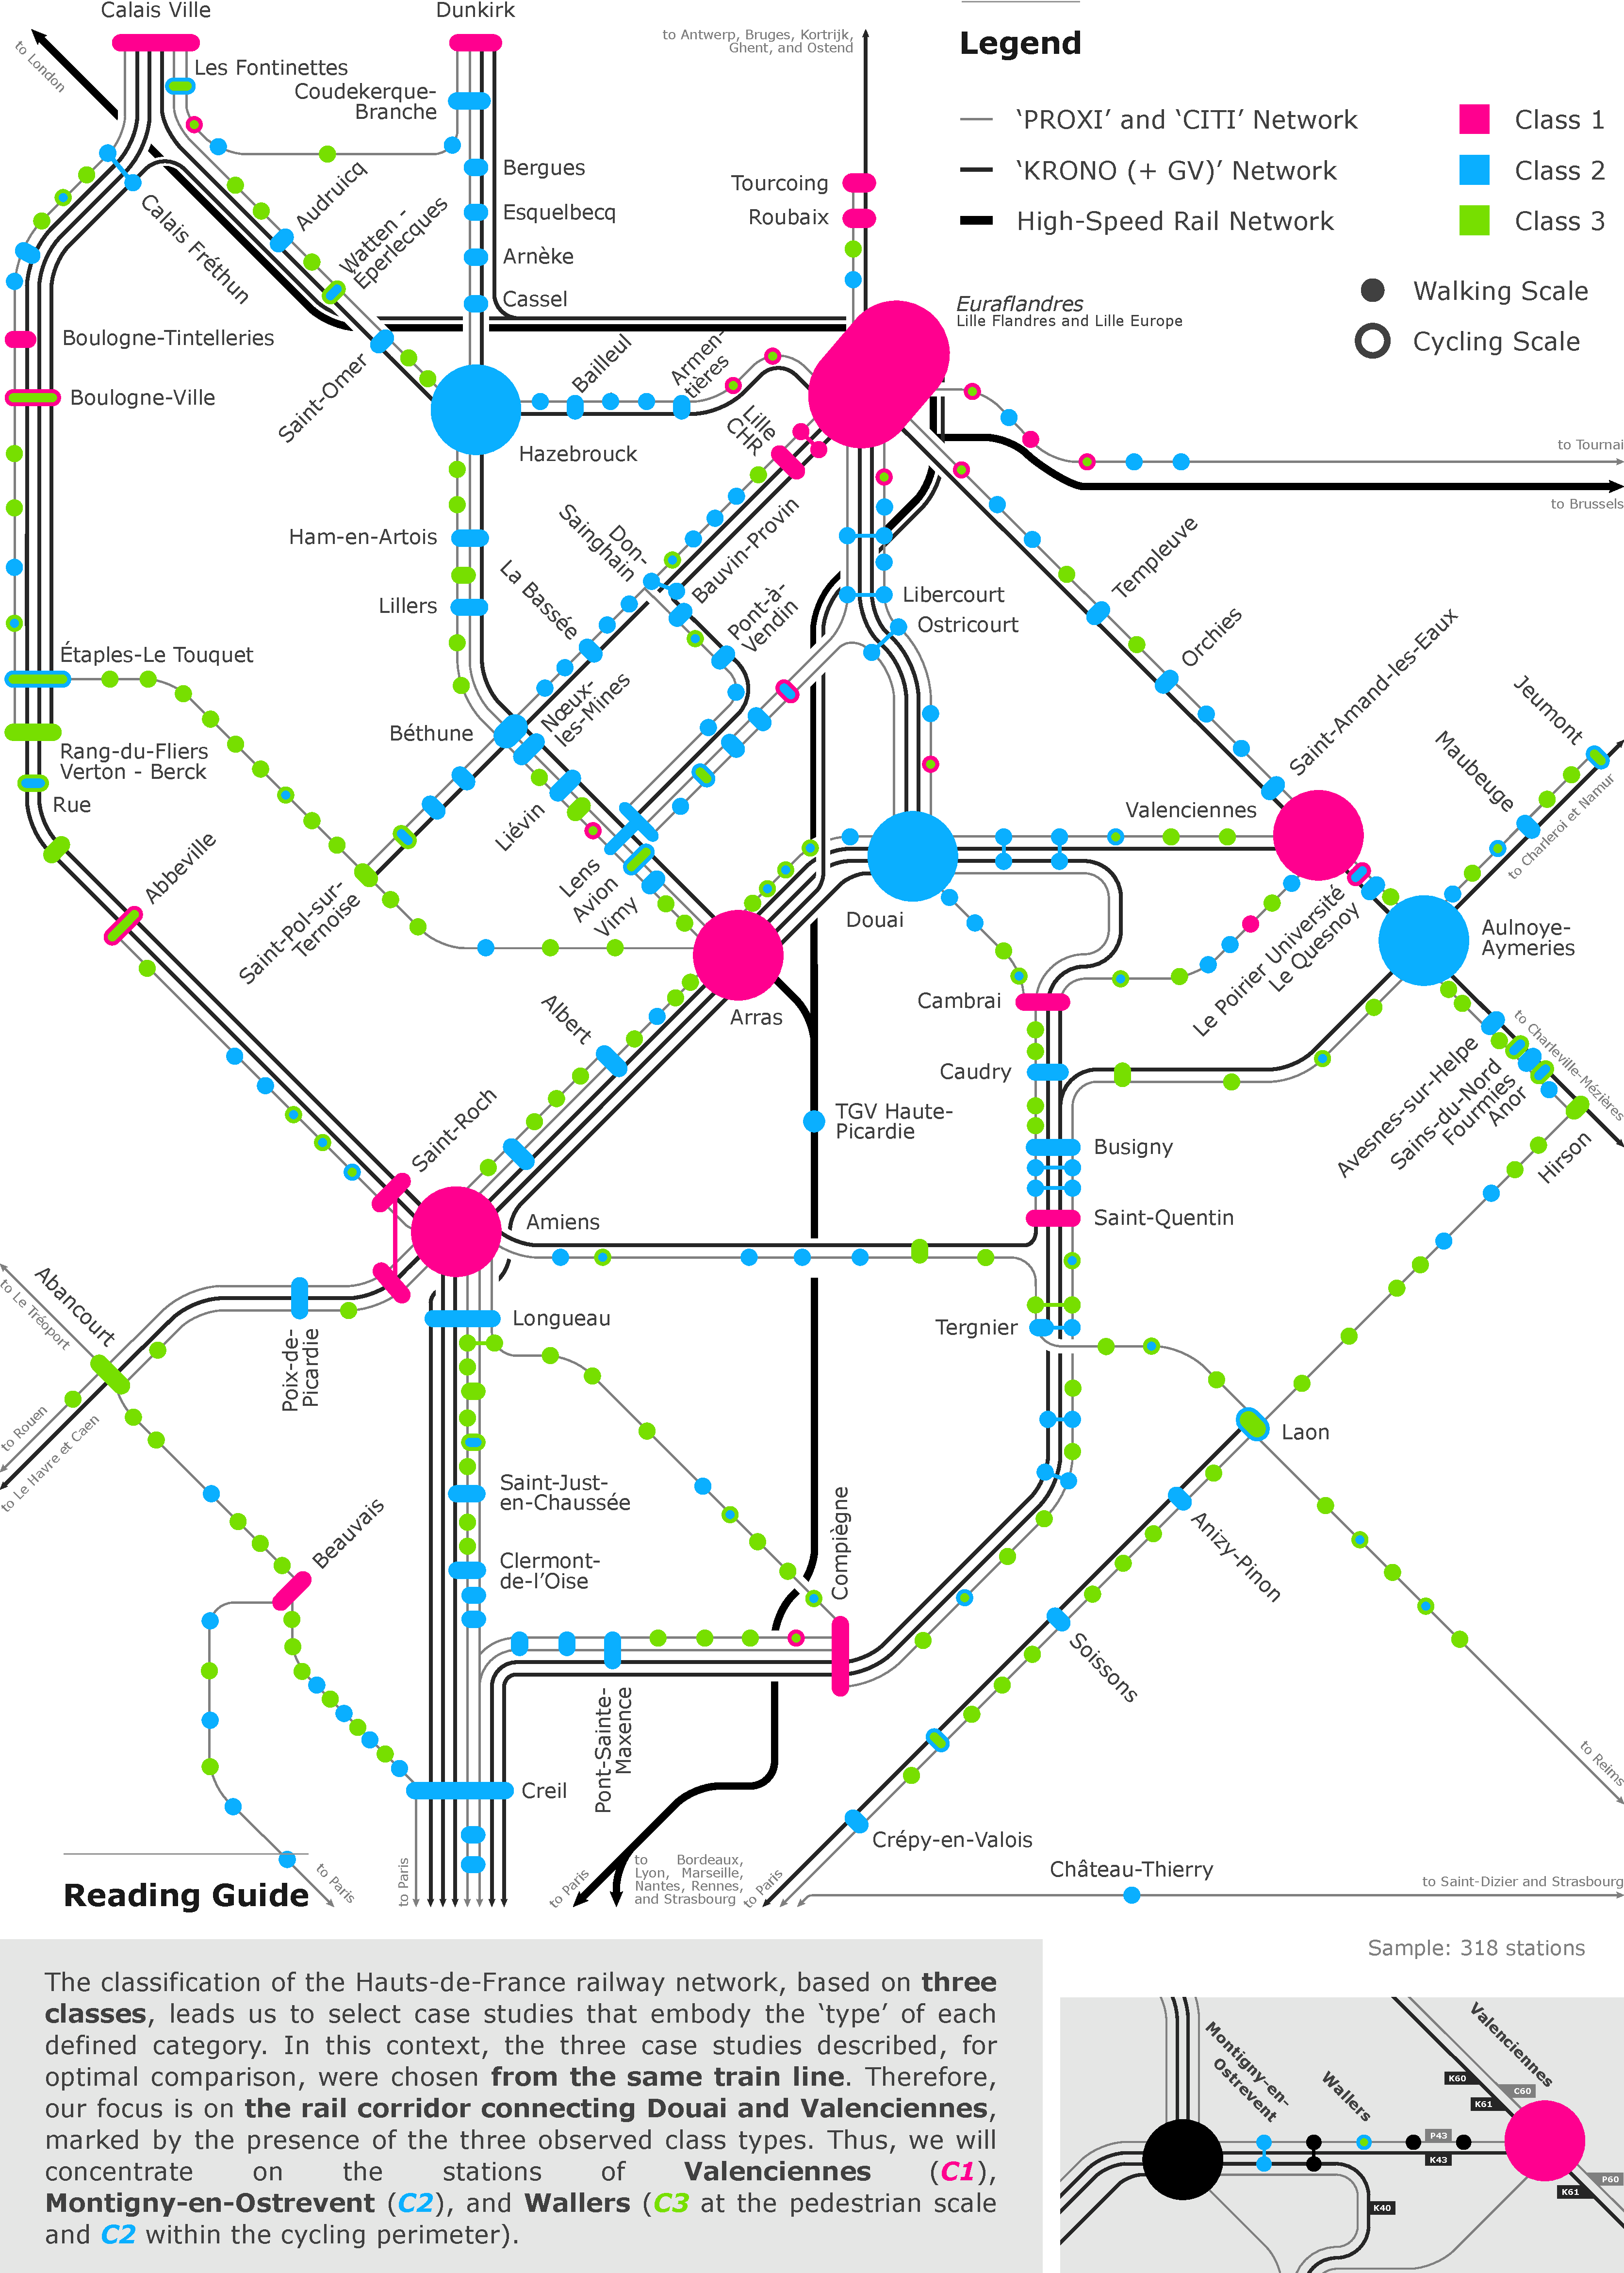
\includegraphics[width=1\columnwidth]{src/Figures/Chap-6/EN_Carte_Reseau_classification.pdf}}
        \vspace{5pt}
        \begin{flushright}\scriptsize{
        Realization: \textcolor{blue}{Dylan Moinse (2024)}
        \\
        Authors: research project \acrshort{NPART}
        }\end{flushright}
    \end{carte}

    % Technical literature
Beyond academic research on the segmentation of stations and their surroundings, it is also important to refer to the study reports produced as part of our regional case study. On a national scale, we can mention the work of \textcolor{blue}{Jean-François} \textcolor{blue}{\textcite[98-104]{troin_essai_2024}}\index{Troin, Jean-François|pagebf}, who proposes a typology of French stations in five categories: the \Commas{metropolitan stations,} the \Commas{specific \acrshort{HST} stations outside the city,} the \Commas{suburban stations,} the \Commas{medium-sized city stations,} and the \Commas{rural stations.} This national categorization, intentionally user-centered, provides insight into the national panorama while engaging with a second segmentation of stations specifically in the Picardy region. We also propose to mention the study reports developed by \textcolor{blue}{\textcite[50-57]{hasiak_pour_2011}}\index{Hasiak, Sophie|pagebf}\index{Bodard, Géraldine|pagebf}\index{Hasiak, Fabrice|pagebf} and \textcolor{blue}{\textcite[6]{cete_nord_picardie_profils_2011}}\index{CETE Nord Picardie@\textsl{CETE Nord Picardie}|pagebf}\index{DREAL Picardie@\textsl{DREAL Picardie}|pagebf} that present various profiles of Picardy stations, based on a set of indicators including the \Commas{transport/mobility} and \Commas{attractiveness and spatial organization} dimensions. These dimensions incorporate themes such as \Commas{service level,} \Commas{station usage,} \Commas{station catchment area,} and \Commas{station environment.} The typology of Picardy stations further distinguishes five classes: the \Commas{regional hub stations}; the \Commas{stations with influence in the Paris region}; the \Commas{stations serving as feeders to regional hubs and Paris}; the \Commas{rural school feeder stations}; and the \Commas{small-town \acrshort{TER} stop points.} While this station distribution is useful for providing an overall portrait, it is more descriptive than strategic. From this perspective, the classification based on \acrshort{NPART} enriches existing knowledge with a more operational framework, allowing public interventions to target specific dimensions based on the classes.%%Translated%%

    % 6.4.3.3.
    \needspace{1\baselineskip} % Réserve de l'espace
\subsubsection*{Case Study of a Railway Corridor
    \label{chap6:results-etudes-de-cas}
    }

    % Introduction
In a decidedly operational perspective, we aimed to enrich spatial modeling by integrating a qualitative analysis based on a selection of case studies. To this end, we chose an exploratory approach to territorial diagnosis, widely used in spatial planning to identify spatial configurations and the specific issues of each site through a sensitive reading of the terrain. This approach, complementary to the quantitative study, draws on the recommendations made in the report on the \acrshort{NPM} in Île-de-France, published by \textcolor{blue}{\textcite[5]{iau_articulation_2017}}\index{IAU@\textsl{IAU}|pagebf}. This document emphasizes the need for a territorial diagnosis to inform and adapt the recommendations to the contextual needs of the planning stakeholders.%%Translated%%

    % C-TOD
In order to adopt a systemic perspective, we focused on the study of a railway corridor, an approach that provides a coherent reading at the scale of a structuring network \textcolor{blue}{\autocite{bairras_slow_2025}}\index{Bairras, Philippe|pagebf}\index{Aguas Ardaiz, Iñigo|pagebf}. This approach is part of the conceptualization of the \acrfull{C-TOD}, developed by \textcolor{blue}{\textcite[17]{liu_conceptual_2020}}\index{Liu, Liwen|pagebf}\index{Zhang, Ming|pagebf}\index{Xu, Tao|pagebf}. Within the framework of our \acrshort{NPART} model, we define a railway corridor as a connection ensured by a direct \acrshort{HST} or \acrshort{TER} line, serving each station without a transfer. To provide an exploratory overview of these territorial diagnoses, we focused our analysis on train station neighborhoods effectively accessible via light individual mobility (\(CI\)), in order to better support our argument and demonstrate the added value of the \acrshort{NPART}. We then deliberately restricted our observations and recommendations to traditional spatial planning tools, considering an implementation in the short or medium term, and excluding any radical restructuring of the built environment, which is seen here as an immutable factor \textcolor{blue}{\autocite[45]{stransky_periurbain_2019}}\index{Stransky, Vaclav|pagebf}.%%Translated%%

    % Etudes de cas
In this regard, we chose to study two train stations located along the railway corridor connecting Douai and Valenciennes: Montigny-en-Ostrevent and Wallers\footnote{~
    Initially, it was planned to include the Valenciennes station in this comparative analysis. However, for reasons of resource efficiency and time feasibility, we decided not to include it. This exclusion is based on several considerations. Firstly, Valenciennes belongs to a category of stations that already tend to or have already reached the expected urban planning model (\(C1\)), which makes it less relevant for our demonstration. Secondly, the class affiliation of this station is relatively narrow in terms of population and well-studied in the literature, so its inclusion would have added limited value. Finally, our results have shown that the potential of the \acrshort{M-TOD} is particularly significant in peri-urban areas, which justifies a focus on Montigny-en-Ostrevent and Wallers, integrated into an intermediate urban system.
} (see \hyperref[fig-chap6:schema-reseau-train-hdf-classes]{Map~\ref{fig-chap6:schema-reseau-train-hdf-classes}}, page~\pageref{fig-chap6:schema-reseau-train-hdf-classes}). This choice is explained by several strategic considerations:
\begin{customitemize}
    \item First, this selection is based on an analysis of the railway corridors connecting the Lille metropolitan area to the cities located south of the regional capital, relying on the conclusions drawn from the doctoral thesis by \textcolor{blue}{Fausto} \textcolor{blue}{\textcite[246]{lo_feudo_scenario_2014}}\index{Lo Feudo, Fausto|pagebf}\index{Menerault, Philippe|pagebf}\index{L'Hostis, Alain|pagebf}\index{Festa, Demetrio Carmine|pagebf}. His research indeed identifies positive scenarios of densification and improvement of public transport offerings for several cities in the Mining Basin, including Béthune, Lens, Douai, Somain, Bouchain, and Denain. The author \Commas{\textsl{clearly shows the possibility of a balancing act where part of the expected urban growth in vast peri-urban areas could be located in the few strategic spaces identified in the regional TOD scenario.}} \textcolor{blue}{\autocite[246]{lo_feudo_scenario_2014}}\index{Lo Feudo, Fausto|pagebf}\index{Menerault, Philippe|pagebf}\index{L'Hostis, Alain|pagebf}\index{Festa, Demetrio Carmine|pagebf};
    \item Next, we chose a monographic approach, allowing us to illustrate each of the classes defined in our typology, except for \(C1\), through a specific case. To ensure balanced representativeness, it was essential to select a railway corridor that includes at least one station from each identified class. After a selection process through elimination, only a few corridors in the southern Lille arc met these criteria;
    \item Furthermore, this selection is part of a forward-looking approach, incorporating a railway corridor that is involved in major transportation infrastructure projects. Thus, we retained an axis benefiting from major transformations induced by the implementation of the \acrfull{SERM} in Lille, promoting a connection with ongoing studies, particularly those being carried out by \textcolor{blue}{\textcite[3]{sncf_gares__connexions_connecter_2024}}\index{SNCF Gares \& Connexions@\textsl{SNCF Gares \& Connexions}|pagebf}, which is developing a diagnostic tool for railway corridors called \Commas{Radar,} designed by the agency \acrfull{AREP}. In their deliverable, several corridors in the Hauts-de-France region are used as examples in their future studies, including the one that includes our two case studies, with a focus on four key dimensions: capacity and safety; service offerings, accessibility, and intermodality;
    \item Another motivation for this choice lies in the desire to avoid being overly influenced by the Lille metropolitan area. Indeed, to prevent the analysis from being biased by the centrality of the \textsl{Euraflandres} exchange hub, we favored a corridor that does not directly reach the \acrshort{MEL}. This orientation allows for a better understanding of the dynamics specific to peri-urban areas and medium-sized cities, which offer more original and revealing experimental grounds for the challenges related to integrating light individual mobility;
    \item Finally, once the corridor was selected, we sought to retain stations that presented indicators close to the median of their class affiliation, to ensure the representativeness of the classification presented. This methodological choice aims to ensure a relevant extrapolation of the results and to identify well-illustrated cases with strong potential for development in terms of sustainable planning and mobility.
\end{customitemize}%%Translated%%

    % Carte Montigny-en-Ostrevent
    \begin{carte}[h!]\vspace*{4pt}
        \caption{Territorial diagnosis of the extended train station neighborhood of Montigny-en-Ostrevent.}
        \label{fig-chap6:monographie-montigny}
        \centerline{\includegraphics[width=1\columnwidth]{src/Figures/Chap-6/EN_NPART_Montigny.png}}
        \vspace{5pt}
        \begin{flushright}\scriptsize{
        Realization: \textcolor{blue}{Dylan Moinse (2025)}
        \\
        Photographs (A), (B), (C), (D), (E), (F), (G), and (H): \textcolor{blue}{Dylan Moinse (2024)}
        \\
        Authors: \acrshort{NPART} Research Project
        }\end{flushright}
    \end{carte}

    % Présentation Montigny-en-Ostrevent
The Montigny-en-Ostrevent station is a particularly interesting case study, located within the Douai urban area and close to the town of Somain. The municipality has approximately 5,000 inhabitants, with a slight population decline since the 1960s. The station is served by the railway line connecting Douai to Valenciennes (P43), as well as by a direct connection between Lille Flandres and Saint-Quentin (K40), providing it with a relatively efficient regional connection. However, the \acrshort{TERGV} of the K43 line, linking Arras to Valenciennes via Douai, does not stop there. Equipped with a passenger building with a ticket counter and an automatic machine, it also has a car park and a secure bike shelter nearby, and is served by bus lines 3; 12 and 108 from the Douai bus network \textsl{Évéole}. Based on the selected analysis criteria and the interpretation of the classes in the \acrshort{NPART}, this station and its surroundings exhibit the characteristics of a \acrshort{TAD} and are classified in \(C2\), both at the pedestrian and cycling scales (see \hyperref[fig-chap6:monographie-montigny]{Map~\ref{fig-chap6:monographie-montigny}}, page~\pageref{fig-chap6:monographie-montigny}).%%Translated%%

    % Diagnostic territorial Montigny-en-Ostrevent - Node
The station records an annual ridership of approximately 130,000 passengers, which is 60\% lower than the regional average (\(RT\)). Regarding rail service, the Montigny-en-Ostrevent station benefits from a relatively high frequency, 38\% higher than the average (\(N_{3}\), 44 \acrshort{TER}); and an extended operating schedule, 7\% higher during weekdays and 16\% higher on weekends (\(N_{5}\) and \(N_{6}\), respectively 16 and 15 hours). Its network also has a higher proximity degree of 35\% (\(N_{10}\)), which supports its strategic position within a connected urban conurbation. Furthermore, the station enjoys easy access to the center of Lille, with a train travel time 29\% shorter and requiring 28\% fewer stops to reach the regional metropolis (\(N_{14}\) and \(N_{15}\), in 30 minutes and 1 stop).%%Translated%%

    % Diagnostic territorial Montigny-en-Ostrevent - Place
However, these advantages in terms of rail service are counterbalanced by less favorable urban development and local connectivity. Although the population density in the cycling catchment area of the Montigny-en-Ostrevent station is comparable to the regional average, the employment density is 44\% lower (\(P_{2}\), 107 jobs per square kilometer), likely due in part to a land use rate dedicated to office and industrial activities that is 70\% lower than the average (\(P_{5}\), 1.2\%). As a result, the station suffers from a limited service offering, with facilities being 23\% fewer for the so-called \Commas{proximity} \acrshort{POIs}, 39\% fewer for \Commas{intermediate} range ones, and 66\% fewer for \Commas{higher} category ones (\(P_{7}\), \(P_{8}\), and \(P_{9}\)). Nevertheless, the station neighborhood stands out for its significant proportion of social housing, more than twice the regional average (\(P_{12}\), 16\%).
%%Translated%%

    % Diagnostic territorial Montigny-en-Ostrevent - Accessibility
Regarding the treatment of public spaces, pedestrian infrastructure is relatively well developed, with a pedestrian infrastructure density 18\% higher than the average for stations (\(A_{1}\), 86 kilometers). Even more notable, the density of the cycling network is particularly high, 188\% higher than the average (\(A_{4}\), 9 kilometers), thus offering a favorable potential for the growth of light individual mobility. Furthermore, the residents of Montigny-en-Ostrevent have a motorization rate 62\% lower (\(A_{11}\), 76\%). However, several limitations should be noted. The provision of bike parking remains insufficient, despite the presence of a bike shelter at the station, with the number of spaces 57\% lower than the regional average (\(A_{5}\), 53 spaces). Additionally, the spatial efficiency of the cycling isochrone—i.e., the actual area accessible compared to its assumed range—is 46\% lower (\(A_{3}\), 18\%). Our field observations confirm that, despite a relatively dense cycling network, it is fragmented and limited to certain sections of departmental roads, often laid out as bike lanes or narrow, uncomfortable tracks. A final critical point lies in the still predominant role of the automobile, both in the organization of the urban fabric and in the distribution of transport infrastructure. This can lead to reflections on the need to accompany railway and cycling urban planning interventions with traffic moderation and road capacity reduction actions. In this regard, it is important to avoid a \Commas{communicating vessels} phenomenon, where the improvement of pedestrian and cycling infrastructure could be partially neutralized by maintaining a road network that still strongly favors cars \textcolor{blue}{\autocite[259]{lo_feudo_scenario_2014}}\index{Lo Feudo, Fausto|pagebf}\index{Menerault, Philippe|pagebf}\index{L'Hostis, Alain|pagebf}\index{Festa, Demetrio Carmine|pagebf}.%%Translated%%

    % Carte Wallers
    \begin{carte}[h!]\vspace*{4pt}
        \caption{Territorial diagnosis of the extended train station neighborhood of Wallers.}
        \label{fig-chap6:monographie-wallers}
        \centerline{\includegraphics[width=1\columnwidth]{src/Figures/Chap-6/EN_NPART_Wallers.png}}
        \vspace{5pt}
        \begin{flushright}\scriptsize{
        Realization: \textcolor{blue}{Dylan Moinse (2025)}
        \\
        Photographs (A), (B), (C), (D), and (E): \textcolor{blue}{Dylan Moinse (2024)}
        \\
        Authors: \acrshort{NPART} Research Project
        }\end{flushright}
    \end{carte}

% Wallers Presentation
The Wallers station constitutes our second case study, which we found interesting due to its complex urban integration, owing to its peripheral location relative to the historical urban fabric of the municipality (see \hyperref[fig-chap6:monographie-wallers]{Map~\ref{fig-chap6:monographie-wallers}}, page~\pageref{fig-chap6:monographie-wallers}). As part of the \acrshort{NPART}, this station appears to be in a state of \Commas{dependence,} both at the pedestrian and cycling levels, due to its low degree of integration with the urban fabric. This train station is exclusively served by a departmental road that crosses the railway line, making it a space poorly integrated into local urban dynamics. As emphasized by the previous \acrfull{PDU} 2013-2023 by \textcolor{blue}{\textcite[78]{siturv_plan_2014}}\index{SITURV@\textsl{SITURV}|pagebf}, although the station is located on the mining spine and benefits from a relatively frequent rail service, its isolation from urban centers detracts from its attractiveness. This situation explains its classification in the last category (\(C3\)) at the pedestrian level (\(PI\)). In contrast, at the cycling level (\(CI\)), the station is more connected, being accessible from the urban center of Wallers as well as from several neighboring municipalities. Thus, at the cycling level, the Wallers station area reaches the second class (\(C2\)). This extension of the Wallers station area, connecting it to the urban area, follows not only the departmental road but also a secondary road network consisting of paths exclusively accessible to active mobility or local residents. Located on the outskirts of the Valenciennes metropolitan area, Wallers is a municipality of approximately 6,000 inhabitants, with a population that has experienced a continuous decline since the 1950s before stabilizing in the 2000s. Only the P43 line, connecting Douai to Valenciennes, makes a stop at Wallers. The station is also served by the 107 and 110 bus lines of the Valenciennes bus network \textsl{Transville}.%%Translated%%

% Wallers Territorial Diagnosis - Node
The annual attendance at the Wallers station is very limited, with 11,000 passengers, accounting for only 3\% of the average attendance at regional stations (\(RT\)). This situation can be attributed to several explanatory factors, including, first and foremost, an improvable service level. The daily train frequency is 29\% lower than the average (\(N_{3}\), 22 \acrshort{TER}), and the station's proximity is slightly reduced, with a level that is 10\% lower (\(N_{10}\)). However, some indicators show more nuanced results. The station has a larger operating range than average, with a 7\% wider range on weekdays and 12\% wider on weekends (\(N_{5}\) and \(N_{6}\), respectively 16 and 14 hours). Furthermore, despite the need to transfer at Valenciennes or Douai, the travel time to Lille remains relatively viable, with a duration 22\% shorter (\(N_{14}\), 50 minutes) and a reduced number of intermediate stops by 17\% (\(N_{13}\), 3 stops). In terms of facilities, the station consists of a rudimentary train stop, characterized by the absence of a true intermodal hub. It includes an old, now unoccupied, passenger building and a ticket machine. In terms of parking infrastructure, it only offers a space for motor vehicles and unmonitored bike racks.%%Translated%%

% Wallers Territorial Diagnosis - Place
However, what most hinders the attractiveness of the Wallers station is the low levels of urban development and design. Despite the potential for expanding its area of influence through light individual mobility, the station only provides access to a sparsely populated urban concentration, where the population density is 38\% lower than the average for stations in the region (\(P_{1}\), 834 inhabitants per square kilometer). Furthermore, its employment density is 56\% lower (\(P_{2}\), 86 jobs per square kilometer), reflecting a marked residential specialization in its cycling station area. This land use, dominated by residential areas, can be seen through the low occupancy rates for industrial activities, which are 61\% lower, and green spaces, which are 78\% lower compared to other stations (\(P_{5}\) and \(P_{6}\), respectively 1.6\% and 0.3\% of land use). We can also observe a scarcity of \acrshort{POIs}, whose presence is 51\% to 90\% lower depending on the categories considered (\(P_{7}\), \(P_{8}\), and \(P_{9}\)), as well as a land value for activities 95\% lower than the regional average (\(P_{11}\),~\euro100 per square meter).%%Translated%%

% Wallers Territorial Diagnosis - Design
In terms of the quality of its public spaces, the Wallers station suffers from a lack of connectivity. The pedestrian network is underdeveloped, with a length of pedestrian spaces 33\% lower than the average (\(A_{1}\), 48 kilometers). Another significant challenge is the deficient provision of cycling infrastructure, with a length 75\% shorter (\(A_{4}\), 1 kilometer). More generally, the road network is poorly interconnected, with 61\% fewer intersections compared to other station neighborhoods (\(A_{2}\), 51 per square kilometer). The lack of dedicated bike infrastructure is therefore a major barrier: it is worth noting that only 16 bike parking spaces are available, 87\% fewer than the average for our sample of stations (\(A_{5}\)). This shortcoming directly affects the attractiveness of the train as an alternative to the car. Nevertheless, some encouraging elements emerge from this exploratory diagnosis: households in the accessible areas are relatively less car-dependent, with a vehicle ownership rate 20\% lower (\(A_{11}\), 68\%). This characteristic highlights an underutilized potential that could be leveraged to encourage a reconfiguration of the station area around walking and light individual mobility, suited to a less motorized population.%%Translated%%

% ___________________________________________
% 6.*.
\newpage
\needspace{1\baselineskip} % Reserve space
\addcontentsline{toc}{section}{Conclusion of Chapter~6}
\sectionheader{Conclusion of Chapter~6}
\section*{Conclusion of Chapter~6
    \label{chap6:conclusion}
    }
    \markright{Conclusion of Chapter~6}{}

% Interest of NPART
Developing station districts often requires prioritizing one aspect or criterion over others, thus raising international debates on \acrshort{TOD} regarding the possibility of simultaneously optimizing a large number of parameters \textcolor{blue}{\autocite[181]{veloso_e_zarate_quartiers_2024}}\index{Veloso e Zarate, Halina|pagebf}\index{Triggianese, Manuela|pagebf}\index{Baron, Nacima|pagebf}\index{Le Bot, Nils|pagebf}\index{Detavernier, Pauline|pagebf}. In this perspective, it is essential to identify the levers of action and their effects to encourage rail-oriented development supported by light individual mobility, in a context where specialized forms of \acrshort{TOD} are emerging \textcolor{blue}{\autocite[111]{cervero_transit-oriented_2017}}\index{Cervero, Robert|pagebf}\index{Guerra, Erick|pagebf}\index{Al, Stefan|pagebf}. It is within this framework that we developed the \acrshort{NPART} model, designed to identify and better understand the mechanisms promoting the development of \acrshort{M-TOD}.%%Translated%%

% Figure Screen GitHub 1
\begin{figure}[h!]\vspace*{4pt}
    \caption{Screenshot of the GitHub repository homepage.}
    \label{fig-chap6:screen-github-1}
    \centerline{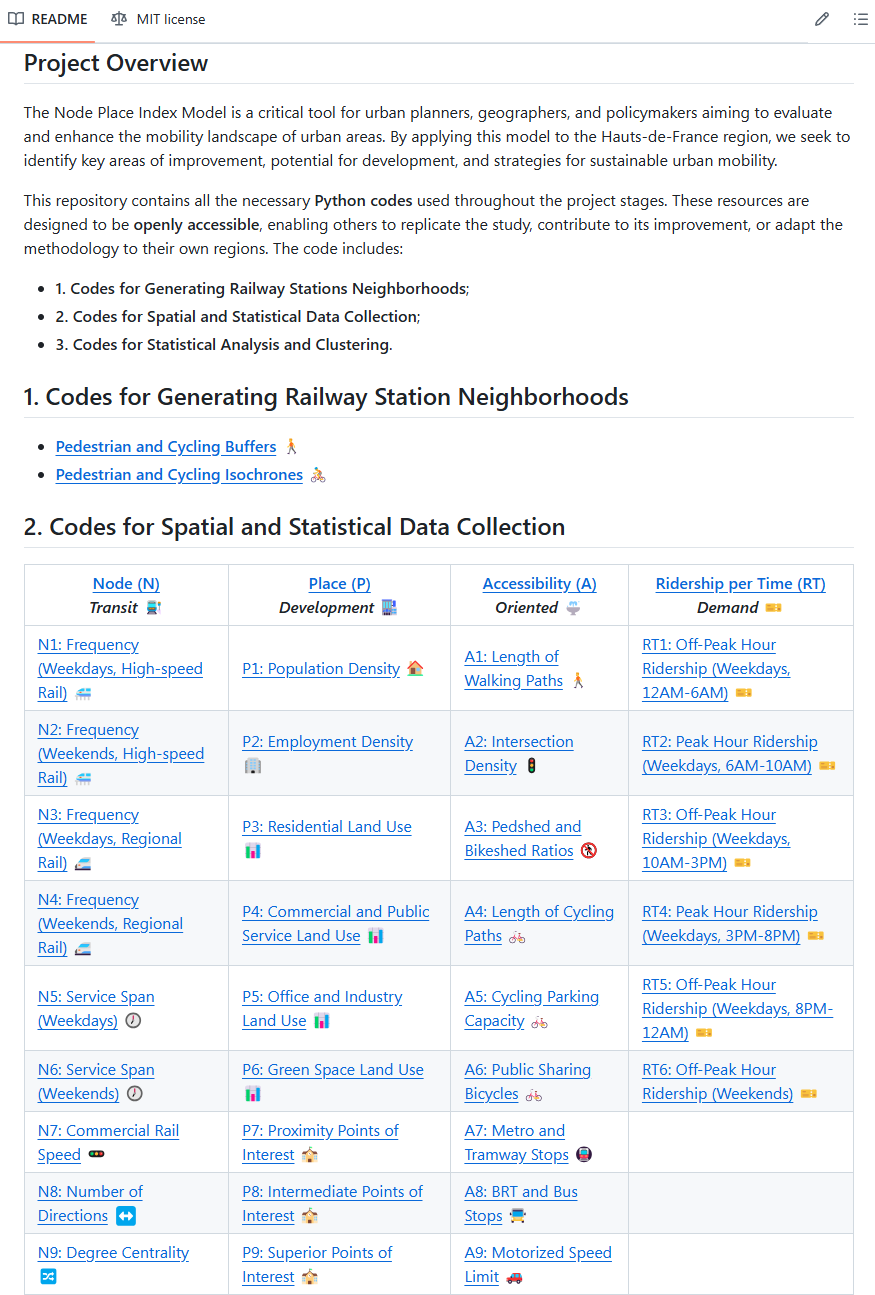
\includegraphics[width=1\columnwidth]{src/Figures/Chap-6/EN_EN_NPART_Screen_Github_1.png}}
    \vspace{5pt}
    \begin{flushright}\scriptsize{
    Realization: \textcolor{blue}{Dylan Moinse (2024)}
    \\
    Authors: \acrshort{NPART} Research Project
    }\end{flushright}
\end{figure}

% Figure Screen GitHub 2
\begin{figure}[h!]\vspace*{4pt}
    \caption{Excerpt from a \textsl{Python} tutorial, formatted in \textsl{Markdown} and made available on \Marque{GitHub}.}
    \label{fig-chap6:screen-github-2}
    \centerline{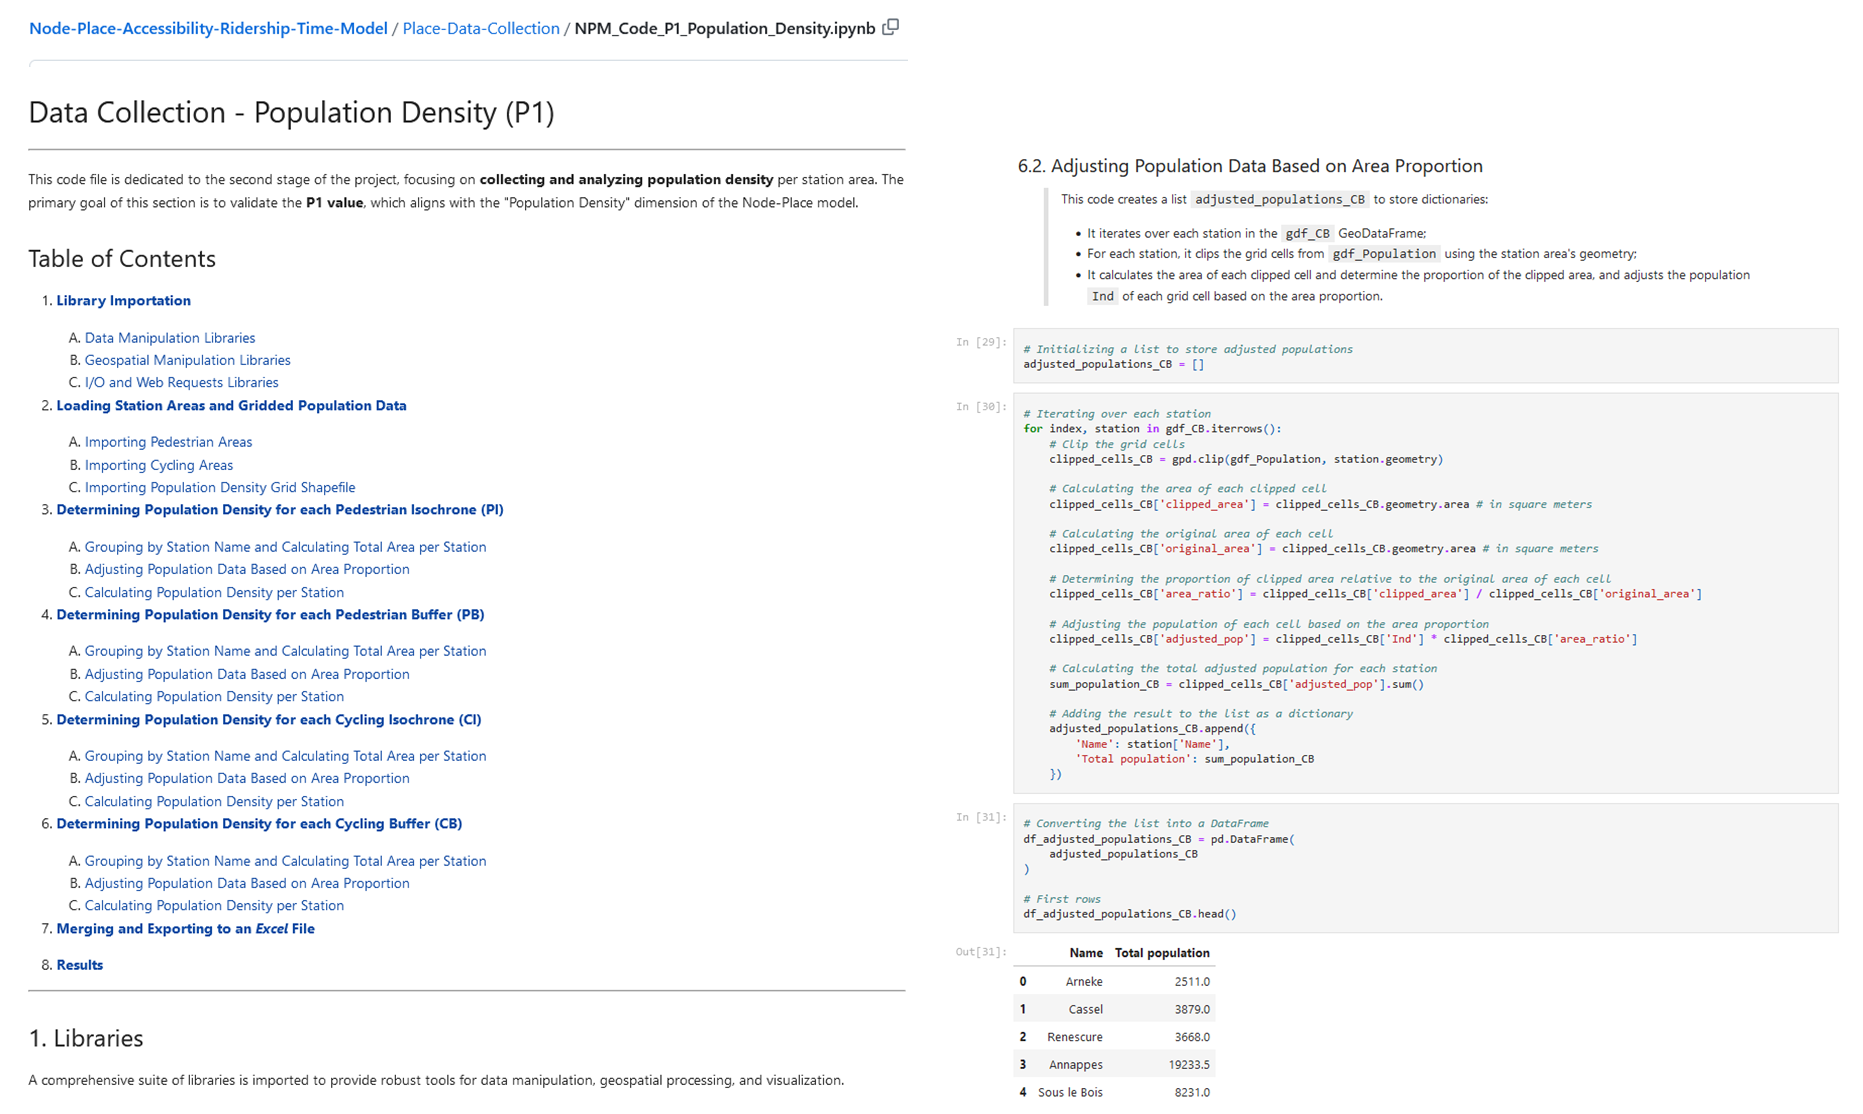
\includegraphics[width=1\columnwidth]{src/Figures/Chap-6/EN_EN_NPART_Screen_Github_2.png}}
    \vspace{5pt}
    \begin{flushright}\scriptsize{
    Realization: \textcolor{blue}{Dylan Moinse (2024)}
    \\
    Authors: \acrshort{NPART} Research Project
    }\end{flushright}
\end{figure}

% 6.*.*
\needspace{1\baselineskip} % Reserve space
\subsection*{Key Findings
    \label{chap6:principaux-enseignements}
    }

% Classification
The classification of stations and their areas of influence has allowed for the identification of three distinct classes, thereby outlining the general profile of the rail network, characterized by a majority of so-called \Commas{dependent} stations, both at the pedestrian and cycling levels. Only 6\% of the stations fall into the class corresponding to \acrshort{TOD}, while nearly half of the network belongs to the category of stations with \acrshort{TOD} potential. It is worth noting that the proportion of stations in the first class, considered as the ultimate goal of urban planning, doubles when station areas are expanded. This highlights the importance of promoting solutions adapted to the \Commas{first and last mile,} such as light individual mobility. Furthermore, the improvement of design, to which cycling contributes significantly, proves to be positively correlated with other dimensions of the model. These interdependencies highlight the strategic role of the connections between the quality of rail service and the degree of urban development, thus confirming the value of an integrated approach to enhance the attractiveness and functionality of serviced areas.%%Translated%%

% M-TOD Criteria
Through this modeling, we have had the opportunity to better define and locate the impact of the main criteria contributing to the definition of a \acrshort{TOD} based on an extended scope of combined walking and \acrshort{M-TOD}. In terms of infrastructure and public transport service, both at the pedestrian and cycling levels, factors such as the frequency of rail service, proximity to centrality, the degree of centrality, the number of directions, and the number of stations accessible within one hour prove to be decisive in increasing station attendance. Regarding activity intensity, criteria such as the land value of industrial, commercial, and office activities, the higher and intermediate \acrshort{POIs}, as well as the presence of green spaces, are among the main components. However, at the cycling level, employment density emerges as an even more dominant factor, ranking at the top of the key indicators. Finally, concerning local connectivity, metro and tram service, as well as elements fostering territorial hospitality towards the development of cycling—such as the presence of \acrshort{PBS}, parking, and cycling facilities—stand out as the most influential factors for both geographical scales. This overview of the main indicators defining this revisited urban strategy also highlights a certain discrepancy with the objectives set by French planners. These planners tend to prioritize access to urban centralities, such as Euralille and Châtelet, the commercial specialization of territories, the development of the pedestrian network, as well as the limitation of motorized speed and car ownership.%%Translated%%

% 6.*.*
\needspace{1\baselineskip} % Reserve space
\subsection*{Valorization of the \acrshort{NPART} Model
    \label{chap6:conclusion-valorisation}
    }

% GitHub
As part of an effort to ensure the reproducibility of the model, we made sure to make the data collection and analysis process entirely transparent by sharing it via a \Marque{GitHub} page\footnote{~
    \Marque{GitHub}~(\url{https://github.com/}) is an online platform for software development management and a service for hosting open-access projects.
} (see \hyperref[fig-chap6:screen-github-1]{Figure~\ref{fig-chap6:screen-github-1}}, page~\pageref{fig-chap6:screen-github-1}). This choice is also aligned with a logic of automation and improved applicability of the model, made possible by the exclusive use of the \textsl{Python} language. The latter not only facilitates the automatic execution of the model but also its adaptation to other geographical and temporal contexts. Thus, the online publication in an environment accessible to a wide community of developers opens new perspectives for the model as an evolving tool, allowing the scientific community and practitioners to explore ways for improvement. To this end, the code has been systematically written in the form of a tutorial (see \hyperref[fig-chap6:screen-github-2]{Figure~\ref{fig-chap6:screen-github-2}}, page~\pageref{fig-chap6:screen-github-2}), to ensure easy reuse and modification by a wide range of users. This approach aims to promote quick and efficient adoption of the analytical tools made available. Beyond mastering the code, this approach also required a constant effort of explanation and pedagogy.%%Translated%%

\bigskip
\begin{tcolorbox}[colback=white!5!white,
                  colframe=blue!75!blue,
                  title=
                  \bigskip
                  \center{GitHub Repository of the \textsl{Node Place Accessibility Ridership per Time} Model}
                  \bigskip]
\center{\normalsize{\url{https://github.com/dylan-moinse/Node-Place-Accessibility-Ridership-Time-Model}}}
\end{tcolorbox}
\bigskip

% Interactive Map
For the purpose of showcasing the model as a practical and interactive visual tool, we developed a draft of a dynamic map, still using the \textsl{Python} programming language. This map could later be enhanced by integrating \textsl{JavaScript}\footnote{~
    \textsl{JavaScript} ensures highly interactive maps, offering a smooth user experience. These maps are accessible without requiring server execution or configuration from the user.
} for increased interactivity. Specifically, it is a mapping tool that allows users to navigate through the different stations in the region and explore the various criteria of the model, both using numerical data and radar charts for \(PI\), \(PB\), \(CI\), and \(CB\). As an illustration, \hyperref[fig-chap6:carte-interactive]{Map~\ref{fig-chap6:carte-interactive}} (page~\pageref{fig-chap6:carte-interactive}) highlights the data related to bike parking (\(A_{6}\)) in the pedestrian (\(PI\)) and cycling (\(CI\)) areas of the Lille CHR station. It shows, on one hand, the available and spatialized offer for each bike parking spot, and on the other hand, this data aggregated at the level of the station districts. The associated radar chart puts this information in perspective with that of other stations, enhancing the readability of the results and facilitating their interpretation in a decision-making or operational context.
%%Translated%%

% Interactive Map
\begin{carte}[h!]\vspace*{4pt}
    \caption{Screenshot of an interactive map displaying bike parking availability around stations.}
    \label{fig-chap6:carte-interactive}
    \centerline{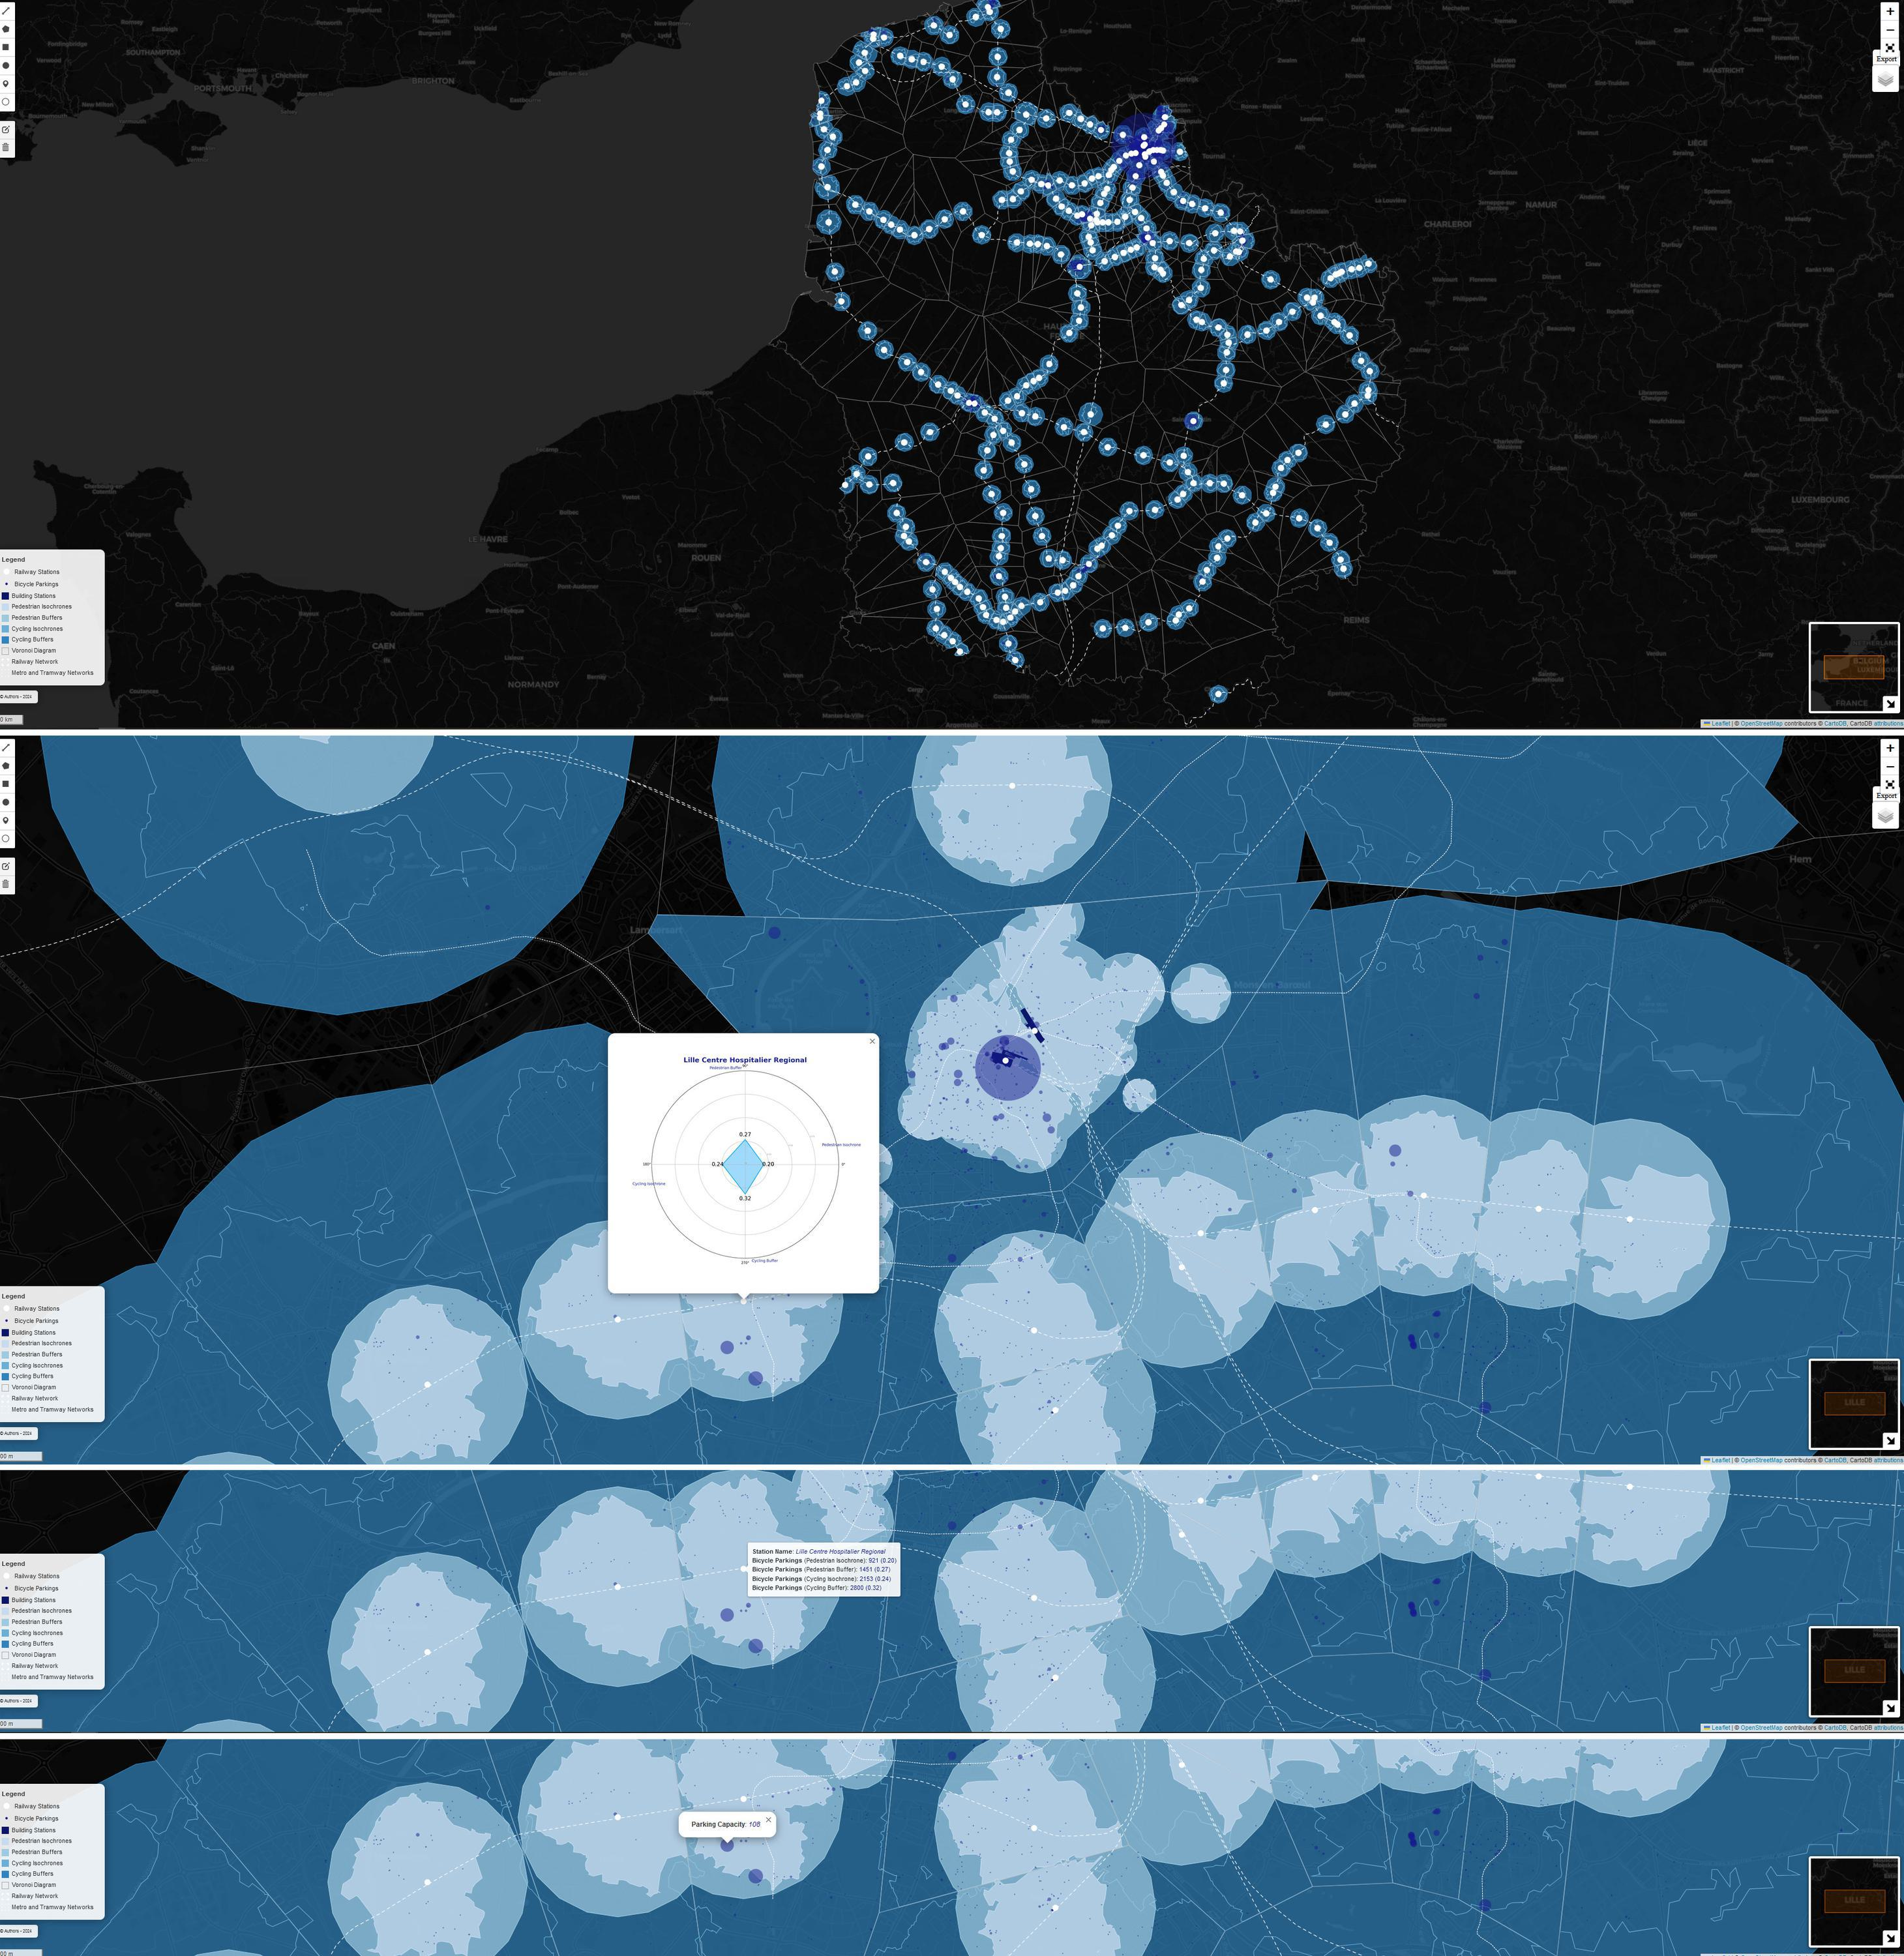
\includegraphics[width=1\columnwidth]{src/Figures/Chap-6/FR_EN_NPART_Carte_interactive.jpeg}}
    \vspace{5pt}
    \begin{flushright}\scriptsize{
    Realization: \textcolor{blue}{Dylan Moinse (2024)}
    \\
    Authors: \acrshort{NPART} Research Project
    }\end{flushright}
\end{carte}

    % Carte fréquence des réseaux de TC
    %\begin{carte}[h!]\vspace*{4pt}
        %\caption{???.}
        %\label{fig-chap6:carte-frequence-reseaux-TC}
        %\centerline{\includegraphics[width=1\columnwidth]{src/Figures/Chap-6/EN_Carte_N1_N2_N3_N4.png}}
        %\vspace{5pt}
        %\begin{flushright}\scriptsize{
        % Réalisation: \textcolor{blue}{Dylan Moinse (2024)}
        % \\
        % Auteur·rice·s: projet de recherche \acrshort{NPART}
        %}\end{flushright}
    %\end{carte}

% Limitations
While the valorization of our model is a key step in ensuring a successful scientific project, we are nevertheless aware of certain limitations. The main constraint in terms of operationalization lies, in our view, in the absence of complete integration of the interviewed planners within the modeling process. Indeed, their role was limited to contributing their opinions in the context of the selection and statistical weighting of the \acrshort{TOD} and \acrshort{M-TOD} criteria. Although we made sure to share the results of this research with them, thus honoring the mutual commitment made with the participants, it would have been beneficial to involve them more by allowing them to test the dynamic map, assess the proposed model, and, more broadly, determine if it aligns with the defined public strategies.%%Translated%%

% Transition to Chapter 7
In this regard, the work of \textcolor{blue}{\textcite[784]{duffhues_breaking_2014}}\index{Duffhues, Jan|pagebf}\index{Mayer, Igor~S.|pagebf}\index{Nefs, Merten|pagebf}\index{Vliet, Mirte van der|pagebf} provides an interesting reference. After conducting a \acrshort{NPM}, these authors invited stakeholders to experiment with their results in the form of a game\footnote{~
    \Commas{Gamification,} or the gamification of research, involves incorporating playful and interactive elements to stimulate engagement, ownership, and motivation of participants, while also enhancing the value of projects conducted by researchers. By integrating game mechanisms, researchers can make their studies more attractive and accessible, particularly for (non) specialized audiences. Gamification thus encourages greater ownership of scientific content by a broader audience \textcolor{blue}{\autocite[6]{genvo_approche_2014}}\index{Genvo, Sébastien|pagebf}\index{Bonenfant, Maude|pagebf}, while the gamification of knowledge training and dissemination processes can strengthen motivation among professionals \textcolor{blue}{\autocite[36, 62]{lu_gamification_2023}}\index{Lu, Huihui|pagebf}. In the context of the \acrshort{NPM} developed by \textcolor{blue}{\textcite[784]{duffhues_breaking_2014}}\index{Duffhues, Jan|pagebf}\index{Mayer, Igor~S.|pagebf}\index{Nefs, Merten|pagebf}\index{Vliet, Mirte van der|pagebf}, a serious game called \textsl{SPRINTCITY} was implemented to simulate the development of a railway corridor over a period of twenty years. Despite some criticisms, it was reported that this game helped raise awareness among stakeholders of the potential benefits offered by \acrshort{TOD}, the strategic importance of the geographical scale of the corridor beyond the station itself, and the conflicts of interest that may arise during the urban planning process.
}. Their observations highlighted that, for these practitioners, the model appeared too focused on a quantitative approach and was difficult to understand, revealing areas for improvement. Based on this insight, the next chapter addresses this limitation by aiming to make the model more tangible and accessible to planners. To do so, we rely on the distinction made by \textcolor{blue}{\textcite[499]{higgins_forty_2016}}\index{Higgins, Christopher~D.|pagebf}\index{Kanaroglou, Pavlos~S.|pagebf}, who differentiate the \Commas{positive} approach—quantitative, systematic, and empirical—from the \Commas{normative} approach, which aims to better describe types of \acrshort{TOD} through qualitative labels. In this perspective, we will illustrate the classification determined from case studies. This approach aims to give a more sensitive and contextual sense, from an urban planning perspective, to the formulated classes by conducting territorial diagnostics and formulating planning proposals at a more granular and contextually adapted geographical scale for each specific case.%%Translated%%

% ___________________________________________
     \newpage
     
% Valorisation scientifique
    \begin{tcolorbox}[colback=white!5!white,
                      colframe=blue!75!blue,
                      title=Valorization
                      \\
                      Chapter~6]
\Large{\textcolor{blue}{\textbf{Congress:}}}
    \\\\
\small{\textcolor{blue}{\textcite{moinse_enhancing_2024}}. Enhancing Transit-Oriented Development with Micromobility: A Renewed Node-Place Index Approach in the Hauts-de-France Region. \textsl{International Geographical Congress} (IGC), \textsl{\Commas{\foreignlanguage{english}{Transport and Geography: Sustainable transit-oriented development (STOD): new perspectives and advances}}}, Dublin.
\\
\footnotesize{\url{https://enpc.hal.science/hal-04682048}} (\textbf{C-ACTI})}
    \\\\
\Large{\textcolor{blue}{\textbf{Communication:}}}
    \\\\
\small{\textcolor{blue}{\textcite{moinse_revisiter_2024}}. Revisiter le modèle de « nœud-lieu » pour évaluer et classifier les quartiers de gare de la région Hauts-de-France. \textsl{Séminaire mensuel du LVMT}, \Commas{Les variations de l'insertion urbaine des gares françaises et leur classification}, Paris.
\\
\footnotesize{\url{https://enpc.hal.science/hal-04620714}} (\textbf{C-COM})}
    \end{tcolorbox}

    % ___________________________________________
    % Subbibliography
    \newpage
    \sectionheader{Bibliography of Chapter~6}
    \begingroup
    \renewcommand{\bibfont}{\scriptsize}
\printbibliography[segment=\therefsegment, heading=subbibintoc, title={Bibliography of Chapter~6}, label=chap6:bibliographie]
    \endgroup
    \end{refsegment}